% ---- ETD Document Class and Useful Packages ---- %
\documentclass{ucetd}

\usepackage{times}
\usepackage{natbib}
\usepackage{fullpage}
\usepackage[utf8]{inputenc}
\usepackage[english]{babel}
\usepackage{amstext,amssymb,amsmath,amsthm}
\usepackage{verbatim}
\usepackage{subfigure}
\usepackage{color}
\usepackage{paralist}
\usepackage{multirow}
\usepackage{listings}
\usepackage{array}
\usepackage{graphicx,color}
\usepackage{moreverb}
\usepackage{xspace}
\usepackage{algorithmic}
\usepackage{algorithm}
\usepackage{times}
\usepackage{relsize}
\usepackage{wrapfig}
\usepackage{enumitem}
\usepackage{mathptmx}
\usepackage{listings}
\usepackage{pgfplots,pgfplotstable}
\usepackage{caption}
\usepackage{subfig}
\usepackage{tikz}

\newcolumntype{x}[1]{>{\centering\arraybackslash}p{#1}}
\newlength\SUBSIZE
\newcommand{\ONECOLFIGMUL}{0.81}
\newcommand{\TALLFIGMUL}{0.75}
\newcommand{\ie}{\textit{i.e.},~}
\newcommand{\eg}{\textit{e.g.},~}
\newcounter{cnt}
\newtheorem{lem}[cnt]{Lemma}
\newtheorem{thm}[cnt]{Theorem}
\newtheorem{problem}[cnt]{Problem}
\newtheorem{defn}[cnt]{Definition}
\newtheorem{fact}[cnt]{Fact}
\newtheorem{example}[cnt]{Example}
\newtheorem{corollary}[cnt]{Corollary}
\newtheorem{assumption}[cnt]{Assumption}
\newtheorem{claim}[cnt]{Claim}
\newcommand{\ip}[2]{\langle #1,#2\rangle}
\renewcommand{\algorithmicrequire}{\textbf{Input:}}
\renewcommand{\algorithmicensure}{\textbf{Output:}}
\newcommand{\nptheta}{\hat\theta}
\newcommand{\symdiff}{\Delta}
\newcommand{\noise}{{\sf Noise}}
\newcommand{\privtheta}{\theta_{priv}}
\renewcommand{\paragraph}[1]{\vspace{3pt}\noindent\textbf{#1}}
\newcommand{\scrX}{\ensuremath{\mathcal{X}}}
\newcommand{\scrZ}{\ensuremath{\mathcal{Z}}}
\newcommand{\rA}{\ensuremath{\rightarrow}}
\newcommand{\rrA}{\ensuremath{\longrightarrow}}
\newcommand{\qB}{\ensuremath{\mathbf{q}}}
\newcommand{\XB}{\ensuremath{\mathbf{X}}}
\newcommand{\zeroB}{\ensuremath{\mathbf{0}}}
\newcommand{\sm}{\mbox{\textendash}}
\newcommand{\ltwo}[1]{\left\|#1\right\|_2}
\newcommand{\lone}[1]{\left\|#1\right\|_1}
\newcommand{\eps}{\epsilon}
\newcommand{\A}{\mathcal{A}}
\newcommand{\D}{\mathcal{D}}
\newcommand{\T}{\mathcal{T}}
\newcommand{\R}{\mathbb{R}}
\newcommand{\K}{\mathcal{K}}
\newcommand{\mineig}{\eta}
\newcommand{\I}{\mathbb{I}}
\newcommand{\E}{\mathbb{E}}
\newcommand{\F}{\mathcal{C}}
\newcommand{\hatw}{\hat{w}}
\newcommand{\hatv}{{\hat{v}}}
\newcommand{\hatV}{{\hat{V}}}
\newcommand{\hatW}{{\hat{W}}}
\newcommand{\kl}{{\sf KL}}
\newcommand{\dagw}{w^\dagger}
\newcommand{\tildew}{\tilde{w}}
\newcommand{\tildeF}{\tilde{F}}
\newcommand{\tildef}{\tilde{f}}
\newcommand{\re}{\mathbb{R}}
\newcommand{\B}{\mathbb{B}}
\newcommand{\bP}{\mathbb{P}}
\renewcommand{\P}{\mathcal{P}}
\newcommand{\grad}{\bigtriangledown}
\newcommand{\mypar}[1]{\smallskip
\noindent{\bf\em {#1}.}}
\newcommand{\etal}{\emph{et al.}}
\newcommand{\negl}{\text{negl}}
\newcommand{\mynote}[3]{\marginpar{\parbox{0.7in}{\tiny {\color{#2} {\sc #1}: {\sf #3}}}}}
\newcommand{\atnote}[1]{\mynote{at}{blue}{#1}}
\newcommand{\nmnote}[1]{\mynote{prmohan}{red}{#1}}
\newcommand{\ignore}[1]{}
\newcommand{\rpm}{\sbox0{$1$}\sbox2{$\scriptstyle\pm$}  \raise\dimexpr(\ht0-\ht2)/2\relax\box2 }

%\newcommand{\TODO}[1]{{\bf TODO: #1}}
\newcommand{\TODO}{}

\newcommand{\NOTE}[1]{{\bf NOTE: #1}}
\newcommand{\name}{\textsc{GUPT}\xspace}
\newcommand{\nameplain}{GUPT\xspace}
\newcommand{\aname}{a \textsc{GUPT}\xspace}
\newcommand{\Aname}{A \textsc{GUPT}\xspace}
\newcommand{\C}{\mathcal{C}}
\newcommand{\hatd}{{\hat d}}
\newcommand{\hatf}{{\hat f}}
\newcommand{\tr}{{\sf tr}}
\newcommand{\Lap}{\mathsf{Lap}}
\newcommand{\M}{\mathcal{M}}
\newcommand{\besta}{a_{{\sf best}}}
\newcommand{\Vect}{\text{vec}}
\newcommand{\Vech}{\text{vech}}
\newcommand{\rank}{\text{rank}}
\newcommand{\diag}{\text{diag}}
\newcommand{\nnz}{\text{nnz}}
\newcommand{\y}{\mathbf{y}}
\newcommand{\w}{\mathbf{w}}
\newcommand{\x}{\mathbf{x}}
\newcommand{\z}{\mathbf{z}}
\newcommand{\cutout}[1]{}
\newcommand{\smallcaption}[1]{\caption[#1]{{\protect\small \protect\bf #1}}}
\newcommand{\dids}{{\sc dids}}
\newcommand{\us}{\,$\mu$s}
\newcommand{\ms}{\,ms}
\newcommand{\KB}{\,KB}
\newcommand{\MB}{\,MB}
\newcommand{\GB}{\,GB}
\newcommand{\MHz}{\,MHz}
\newcommand{\GHz}{\,GHz}

\definecolor{gray}{gray}{0.75}
%\newcommand{\TODO}[1]{\textcolor{gray}{\textbf{\ [TODO:\ #1]\ }}}
\newcommand{\secref}[1]{Section~\ref{sec:#1}}
\newcommand{\Secref}[1]{Section~\ref{#1}}
\newcommand{\PUNT}[1]{}
\newcommand{\figref}[2][{}]{{Figure~\ref{#2}#1}}
\newcommand{\figsref}[2]{Figures~\ref{#1} and~\ref{#2}}
\newcommand{\tblref}[1]{Table~\ref{tbl:#1}}
\newcommand{\algref}[1]{Algorithm~\ref{alg:#1}}
\renewcommand{\textfraction}{0.05}
\newcommand{\figrref}[2]{Figures~\ref{#1}--\ref{#2}}
\newcommand{\secsref}[2]{Sections~\ref{sec:#1} and~\ref{sec:#2}}
\newcommand{\eqnref}[1]{Eqn.~\ref{eqn:#1}}
\newcommand{\eqnsref}[2]{Eqns.~\ref{eqn:#1} and~\ref{eqn:#2}}
\newcommand{\eqnrref}[2]{Eqns.~\ref{eqn:#1}--\ref{eqn:#2}}
\newcommand{\appref}[1]{Appendix~\ref{app:#1}}
\renewcommand{\paragraph}[1]{\vspace{3pt}\noindent\textbf{#1}}
\newcommand{\st}{s.t.}
%\DeclarePairedDelimiter\Floor\lfloor\rfloor
%\DeclarePairedDelimiter\Ceil\lceil\rceil
\DeclareMathOperator*{\argmin}{arg\,min}
\DeclareMathOperator*{\minimize}{min}
\DeclareMathOperator*{\argmax}{arg\,max}
\DeclareMathOperator*{\Floor}{\lfloor\rfloor}
\DeclareMathOperator*{\Ceil}{\lceil\rceil}

\definecolor{mygreen}{rgb}{0,0.6,0}
\definecolor{mygray}{rgb}{0.5,0.5,0.5}
\definecolor{mymauve}{rgb}{0.58,0,0.82}

\definecolor{on}{RGB}{159, 169,133}
\definecolor{off}{RGB}{255,165,0}%{240,232,205}
\definecolor{leo}{RGB}{72,181,163}
\definecolor{poet}{RGB}{249,140,182}
\definecolor{calnp}{RGB}{117,137,191}
\definecolor{cal}{RGB}{51,255,51} %green


\definecolor{OPTIMAL}{RGB}{0,0,0}
\definecolor{RACE}{RGB}{251,128,114}
\definecolor{CONTROL}{RGB}{255,237,111}
\definecolor{ONLINE}{RGB}{253,180,98}
\definecolor{OFFLINE}{RGB}{252,205,229}
\definecolor{NETFLIX}{RGB}{217,217,217}
\definecolor{HBM}{RGB}{190,186,218}
\definecolor{POET}{RGB}{188,128,189}
\definecolor{CALOREE-NP}{RGB}{179,222,105}
\definecolor{CALOREE-ONLINE}{RGB}{204,235,197}
\definecolor{CALOREE-NETFLIX}{RGB}{141,211,199}
\definecolor{CALOREE-HBM}{RGB}{128,177,211}
\definecolor{PID-CONTROL}{RGB}{255,237,111}
\definecolor{NUCLEAR}{RGB}{190,186,218}
\definecolor{ADAPT-CONTROL}{RGB}{188,128,189}
\definecolor{ONLINE-ADAPT}{RGB}{204,235,197}
\definecolor{NUCLEAR-ADAPT}{RGB}{141,211,199}
\definecolor{HBM-ADAPT}{RGB}{128,177,211}


\lstset{ %
  backgroundcolor=\color{white},   % choose the background color; you must add \usepackage{color} or \usepackage{xcolor}
  basicstyle=\scriptsize\ttfamily, % the size of the fonts that are used for the code
  breakatwhitespace=false,         % sets if automatic breaks should only happen at whitespace
  breaklines=true,                 % sets automatic line breaking
  captionpos=b,                    % sets the caption-position to bottom
  commentstyle=\color{mygreen},    % comment style
  deletekeywords={...},            % if you want to delete keywords from the given language
  escapeinside={\%*}{*},          % if you want to add LaTeX within your code
  extendedchars=true,              % lets you use non-ASCII characters; for 8-bits encodings only, does not work with UTF-8
  frame=leftline,                  % adds a frame around the code
  keepspaces=true,                 % keeps spaces in text, useful for keeping indentation of code (possibly needs columns=flexible)
  keywordstyle=\color{blue},       % keyword style
  morekeywords={*,...},            % if you want to add more keywords to the set
  numbers=left,                    % where to put the line-numbers; possible values are (none, left, right)
  numbersep=5pt,                   % how far the line-numbers are from the code
  numberstyle=\tiny\color{mygray}, % the style that is used for the line-numbers
  rulecolor=\color{black},         % if not set, the frame-color may be changed on line-breaks within not-black text (e.g. comments (green here))
  showspaces=false,                % show spaces everywhere adding particular underscores; it overrides 'showstringspaces'
  showstringspaces=false,          % underline spaces within strings only
  showtabs=false,                  % show tabs within strings adding particular underscores
  stepnumber=1,                    % the step between two line-numbers. If it's 1, each line will be numbered
  stringstyle=\color{black},     % string literal style
  tabsize=1,                       % sets default tabsize to 2 spaces
  title=\lstname                   % show the filename of files included with \lstinputlisting; also try caption instead of title
}


% options for pgfplots
\pgfplotsset{compat=1.8,compat/show suggested version=false}
\usetikzlibrary{calc,trees,arrows,patterns,plotmarks,shapes,snakes,er,3d,automata,backgrounds,topaths,decorations.pathmorphing,decorations.markings}
%\pgfplotsset{compat=newest}
\pgfplotsset{
   /pgfplots/bar  cycle  list/.style={/pgfplots/cycle  list={%
        {black,fill=black!30!white,mark=none},%
        {black,fill=red!30!white,mark=none},%
        {black,fill=green!30!white,mark=none},%
        {black,fill=yellow!30!white,mark=none},%
        {black,fill=brown!30!white,mark=none},%
     }
   },
}
% begin of externalization
\usetikzlibrary{external}
\tikzexternalize[prefix=out/]
\tikzexternalize
\usetikzlibrary{patterns}
\usepgfplotslibrary{groupplots}

\usepackage{tikz}

%\usepgfplotslibrary{groupplots}
\usetikzlibrary{pgfplots.groupplots}


\pgfplotsset{
every axis label/.append style={font=\footnotesize},
tick label style={font=\footnotesize},
compat=1.13
}

\makeatletter
\g@addto@macro\normalsize{%
  \setlength\abovedisplayskip{4pt plus 2pt minus 1pt}
  \setlength\belowdisplayskip{4pt plus 2pt minus 1pt}
  \setlength\abovedisplayshortskip{4pt plus 2pt minus 1pt}
  \setlength\belowdisplayshortskip{4pt plus 2pt minus 1pt}
}
\makeatother

\newif{\ifanonymous}
\anonymoustrue

\newcommand{\SYSTEM}{CALO\-REE}
%\newcommand{\SYSTEM2}{CALO\-REE}
%% Use these commands to set biographic information for the title page:
\title{Statistical Methods for Performance Estimation for Improving Scheduling and Energy Minimization}
\author{Nikita Mishra}
\department{Computer Science}
\division{Physical Science Division}
\degree{Doctor of Philosophy}
\date{June 10, 2017}

%% Use these commands to set a dedication and epigraph text
\dedication{Dedication Text}
\epigraph{Epigraph Text}
\bibliography{reference}
\bibliography{references}


\begin{document}
%% Basic setup commands
% If you don't want a title page comment out the next line and uncomment the line after it:
\maketitle
%\omittitle

% These lines can be commented out to disable the copyright/dedication/epigraph pages
\makecopyright
\makededication
\makeepigraph
%% Make the various tables of contents
\tableofcontents
\listoffigures
\listoftables
\graphicspath{{figures/}} % Location of the graphics files
%\graphicspath{{Figures/}} % Location of the graphics files

\acknowledgments
% Enter Acknowledgements here

\abstract
% Enter Abstract here
\begin{abstract}
  This thesis is about using statistical methods for performance and power estimation which would allow us to develop better
  scheduling algorithms and also more energy efficient systems.
  In many deployments, computer systems are underutilized – meaning that
  applications have performance requirements that demand less than full
  system capacity. Ideally, we would take advantage of this under-utilization
  by allocating system resources so that the performance requirements are met
  and energy is minimized. This optimization problem is complicated by the fact
  that the performance and power consumption of various system configurations
  are often application – or even input – dependent. Thus, practically,
  minimizing energy for a performance constraint requires fast, accurate
  estimations of application-dependent performance and power tradeoffs. We propose
  a set of algorithms for different scenarios to tackle this problem.
First, we propose LEO, a probabilistic graphical model-based learning system that
  provides accurate online estimates of an application’s power and performance
  as a function of system configuration. This work mostly focuses on the performance estimation
  for single applications. As the second part of our work, we design a system called CALOREE which allows
  the learnt models to be combined with a controller so that the system is robust
  to dynamic situations with changing resource requirement. Finally, as the third
  part of our work, we look into the estimation for application’s performance when
  they are co-scheduled with other applications.  Applications co-scheduled on the same physical hardware interfere with one
  another by contending for shared resources. Predicting this interference ahead of time would be particularly valuable for
  job scheduling. We therefore propose an efficient technique for estimating application interference
  based on sparse regression. We call our approach ESP for Estimating co-Scheduled Performance.

  LEO uses a graphical model to integrate a small number of observations of the current application with
knowledge of the previously observed applications to produce accurate estimations of
power and performance trade-offs for the current application in all configurations.
LEO produces the most accurate estimates and near optimal energy savings.
These estimates can greatly resource allocation in static situation.
But the second major challenge in real systems is \textit{dynamics}, dynamics—performance must
be maintained despite unpredictable changes in operating environment or input.
Machine learning accurately predicts the performance of complex, interacting resources, but does not address
system dynamics; control theory adjusts resource usage dynamically, but
   struggles with complex resource
   interaction. We therefore propose CALOREE, a combination of learning and control
   that automatically adjusts
   resource usage to meet performance requirements with minimal energy in complex, dynamic environments.
   CALOREE breaks resource allocation into two sub-tasks: learning speedup as a function of resource usage, and
   controlling speedup to meet performance requirements. CALOREE also defines a general interface allowing
   different learners to be combined with a controller while maintaining control’s formal guarantees that
   performance will converge to the goal. We implement CALOREE and test its ability to deliver reliable
   performance on heterogeneous ARM big.LITTLE architectures in both single and multi-application scenarios.
   Compared to state-of-the-art learning and control solutions, we find that CALOREE reduces deadline misses
   by 2–6x while reducing energy consumption by 7–10\%.
Finally, the additional challenge that real systems face is performance loss due
to application interference. We quantify interference as slowdown, or the performance loss one application
   experiences in the presence of co-scheduled applications.
    Given an accurate interference prediction, a scheduler can determine
   optimal assignments of applications to physical machines, leading to higher throughput
   in batch systems and better quality-of-service for latency-sensitive applications.
   In data centers and super computers schedulers often have a great deal of accumulated
   data about past jobs and their interference, yet turning this data into effective
   interference predictors is difficult.
   We explore such state-of-the-art regularized regression models for estimating
   application interference. We find that regularized linear regression methods
   require a relatively small number of features, but produce inaccurate models.
   In contrast, non-linear models that include interaction terms – i.e., permit
   features to be multiplied together – are more accurate, but are extremely inefficient
   and not practical for online scheduling.
The key insight in ESP is to split regression modeling into two parts: feature
   selection and model building. ESP uses linear techniques to perform feature selection,
   but uses quadratic techniques for model building. The result is a highly accurate
   predictor that is still practical and can be integrated into a real application scheduler.
\end{abstract}

\mainmatter

\chapter{Single Application power and performance}
%Title: \SYSTEMLEO{}: A machine learning approach to minimizing energy under performance constraints

\section{Introduction}

% Two trends: energy and load variations
This work addresses two trends in modern computing systems.  First,
energy is increasingly important; reducing energy consumption reduces
operating costs in datacenters and increases battery life in mobile
devices.  Second, computer systems are often underutilized, meaning
there are significant portions of time where application performance
demands do not require the full system capacity
\cite{google2007,MeisnerISCA2011}.

% Problem: How to minimize energy while meeting load demands
These two trends raise the problem of allocating available resources
to meet the current performance demand while minimizing energy
consumption. This problem is a \emph{constrained optimization}
problem. The current utilization level represents a performance
constraint (\ie an amount of work that must be completed in a given
time); system energy consumption represents the objective function to
be minimized.

% Prior approaches: heuristics (race-to-idle) and convex optimization
This problem is challenging because it requires a great deal of
knowledge to solve.  More than knowledge of the single fastest, or
most energy efficient system configuration solving this problem
requires knowledge of the power and performance available in all
configurations and the extraction of those configurations that
represent Pareto-optimal tradeoffs.  Acquiring this knowledge is
additionally complicated by the fact that these power/performance
tradeoffs are often application -- or even input -- dependent.  Thus,
there is a need for techniques that accurately estimate these
application-dependent parameters during run-time.

Machine learning techniques represent a promising approach to
addressing this estimation problem.  \emph{Offline learning}
approaches collect profiling data for known applications and use that
to predict optimal behavior for unseen applications (examples include
\cite{Yi2003,Koala,LeeBrooks2006,CPR,ChenJohn2011}).  \emph{Online
  learning} approaches use information collected while an application
is running to quickly estimate the optimal configuration (examples
include
\cite{Li2006,Flicker,ParallelismDial,Ponamarev,petabricksDynamic,LeeBrooks,TAAS}).
Offline methods require minimal runtime overhead, but suffer because
they estimate only trends and cannot adapt to particulars of the
current application.  Online methods customize to the current
application, but cannot leverage experience from other applications.
In a sense, offline approaches are dependent on a rich training set
that represents all possible behavior, while the online approaches
generate a statistically weak -- \ie inaccurate -- estimator due to
small sample size.

In this work, we present \SYSTEMLEO{} (Learning for Energy
Optimization), a learning framework that combines the best of both
worlds, \ie the statistical properties both offline and online
estimation.  We assume that there is some set of applications for
which the power and performance tradeoffs are gathered offline.
\SYSTEMLEO{} uses a graphical model to integrate a small number of
observations of the current application with knowledge of the
previously observed applications to produce accurate estimations of
power and performance tradeoffs for the current application in all
configurations.  \SYSTEMLEO{}'s strength is that it quickly matches the
behavior of the current application to a subset of the previously
observed applications.  For example, if \SYSTEMLEO{} has previously seen
an application that only scales to 8 cores, it can use that
information to quickly determine if the current application will be
limited in its scaling.


% Limitations and uses \TODO{Need to have a paragraph here on
%   limitations - but keep it positive.}
\SYSTEMLEO{} is a fairly general approach in that it supports many types
of applications with different resource needs.  It is not, however,
appropriate for all computer systems, especially ones, which run many
small, unique jobs.  Instead, it focuses on supporting systems that 1)
execute longer running jobs (in the 10s of seconds) or many repeated
instances of short jobs, 2) run at a wide range of utilizations, and
3) might have phases where optimal tradeoffs may change online.  For
systems that meet these criteria, \SYSTEMLEO{} provides a powerful
ability to reduce the energy consumption.  For systems that service
short ( $< 1$ second), largely unique jobs, \SYSTEMLEO{} will work, but
other approaches are probably better matched to those specific needs.
%\TODO{its probably alright for full utilization systems too because it can tell which configuration provides maximum utilization. Also, race-to-idle is not mentioned in intro?}

% Our results
We have implemented \SYSTEMLEO{} on a Linux x86 server and tested its
ability to minimize energy for 25 different applications from a
variety of different benchmark suites.  We first compare \SYSTEMLEO{}'s
performance and power prediction accuracy to (1) the true value, (2)
an offline approach, and (3) an online approach (See
\Secref{sec:poc}).  On average, \SYSTEMLEO{} is within 97\% of the true
value while the offline and online approaches only achieve 79\% and
86\% accuracy, respectively.  We then use \SYSTEMLEO{} to minimize energy
for various performance requirements (or system utilizations) (See
\Secref{sec:experiment:LP}).  Overall we find that our approach is
within 6\% of the true optimal energy, while the offline approach
exceeds optimal energy consumption by 29\% and online approach by
24\%.  Finally, we show that \SYSTEMLEO{} provides near optimal energy
savings when adapting to phases within an application.

% Contributions of this work
This work makes the following contributions:
\begin{itemize}
\item To the best of our knowledge, this is the first application of
  probabilistic graphical models for solving crucial system
  optimization problems such as energy minimization.
\item It presents a graphical model capable of accurately
  estimating the application-specific performance and power of
  computer system configurations without prior knowledge of the
  application. (See \Secref{sec:HBN}).
\item It makes the source code for this learning system available in
  both Matlab and C++\footnote{leo.cs.uchicago.edu}.
\item It evaluates \SYSTEMLEO{} on a real system. (See
  \Secref{sec:experiment}).
\item It compares the accuracy of \SYSTEMLEO{}'s estimations to both the
  truth and to offline and online learning approaches (See
  \Secref{sec:experiment:PP}).
\item It integrates \SYSTEMLEO{} into a runtime for energy optimization
  and finds this learning framework achieves near-optimal energy
  savings.  Furthermore, \SYSTEMLEO{} significantly reduces energy
  compared to both offline and online approaches as well as the
  popular race-to-idle heuristic.  (See
  \Secref{sec:experiment:LP}).
\end{itemize}

The rest of the work is organized as follows. \Secref{sec:example}
provides a motivational example to build intuition.
\Secref{sec:notation} presents notation.
\Secref{sec:problemFormulation} formalizes the energy minimization
problem as a linear program and discusses the application-specific
parameters of this problem.  \Secref{sec:HBN} elaborates our probabilistic graphical model and describes \SYSTEMLEO{} in full detail.
\Secref{sec:experiment} presents empirical studies on \SYSTEMLEO{}.
Related work is discussed in \Secref{sec:related} and the work
concludes in \secref{conclusion}.


\section{Motivational Example}
\label{sec:example}
\begin{figure*}
\begin{center}
\begin{tabular}[t!]{ccc}\hspace*{-15pt}
	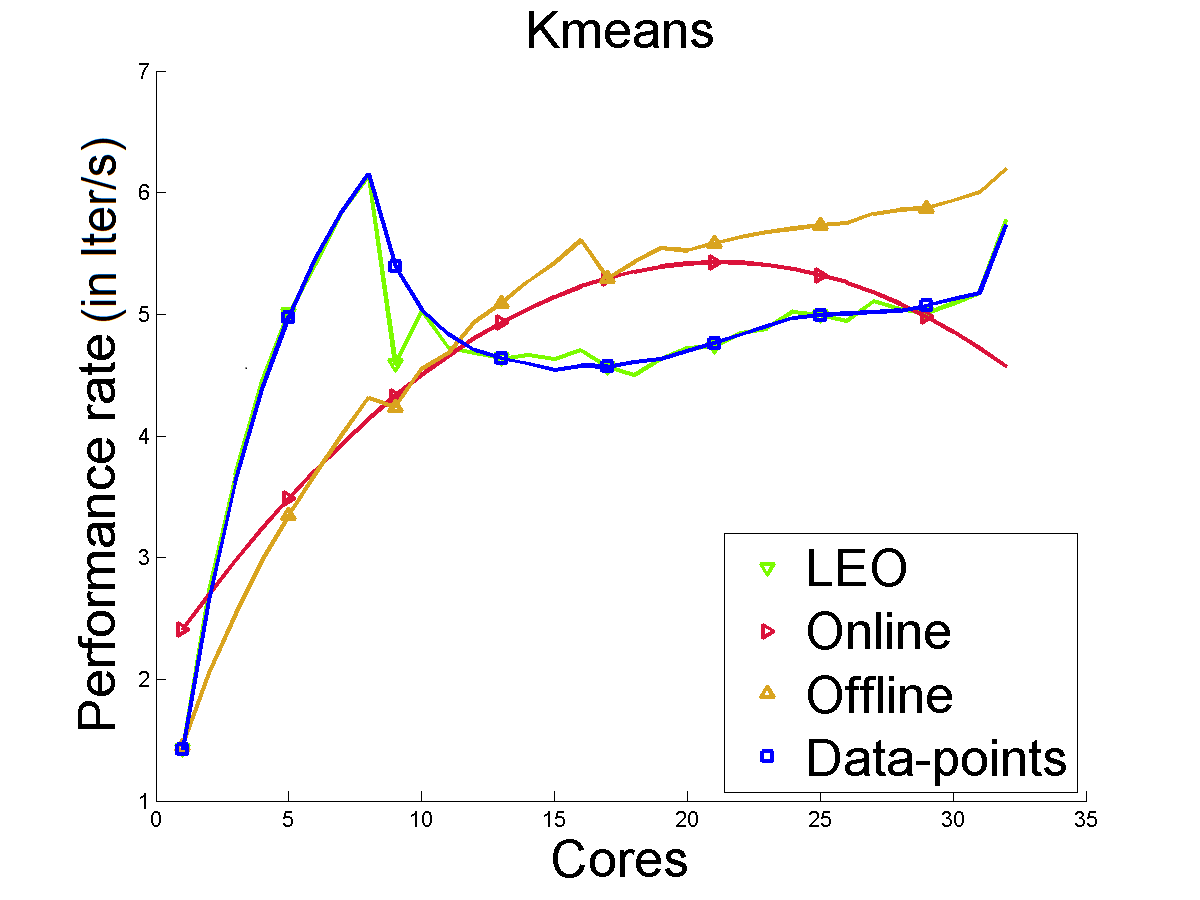
\includegraphics[width=0.3\textwidth]{KmeansCoresPerf.png}&
	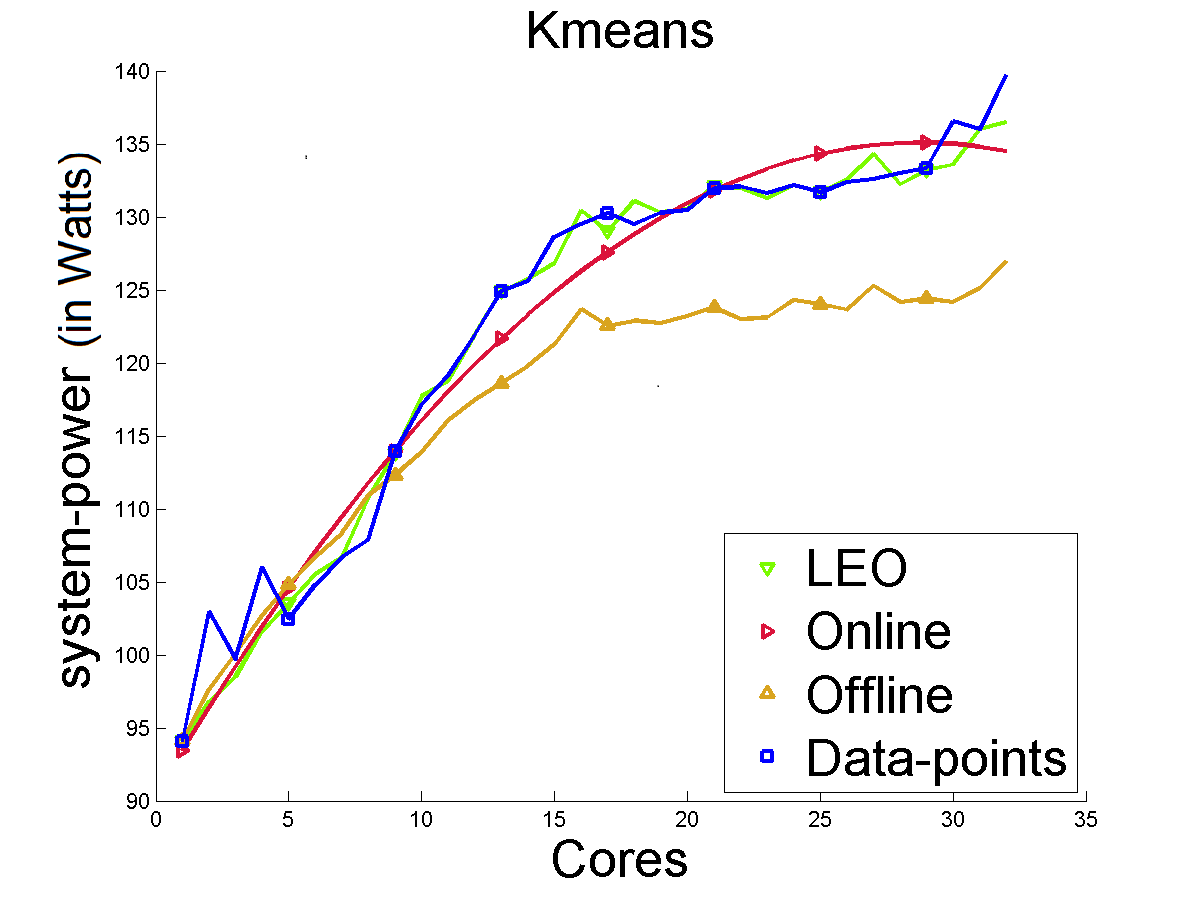
\includegraphics[width=0.3\textwidth]{KmeansCoresPower.png}&
	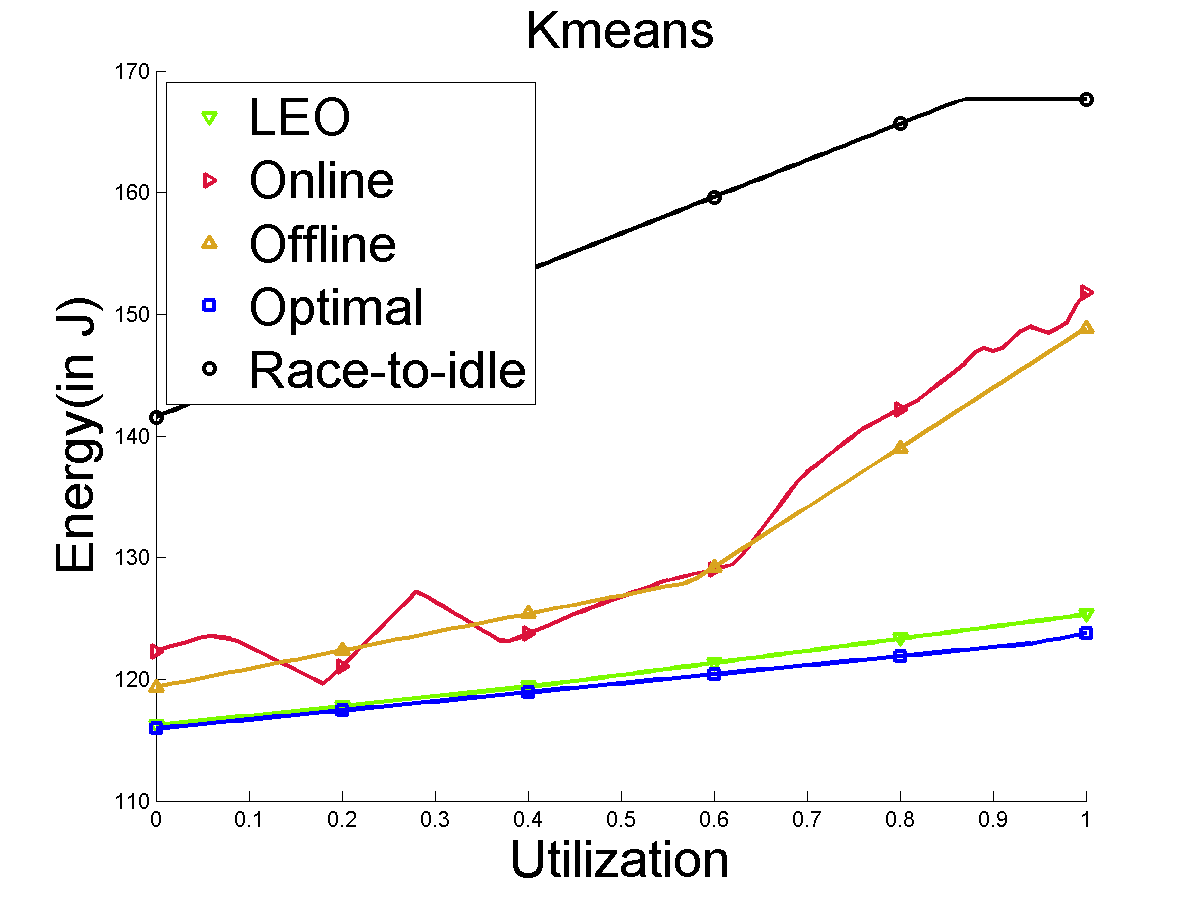
\includegraphics[width=0.3\textwidth]{KmeansCoresEnergy.png}\\
	 {(a)} &
	 {(b)} &
	  {(c)}
\end{tabular}
\vspace{-0.35em}
\caption{Power estimation for \texttt{Kmeans}
  clustering application using \SYSTEMLEO{}, \textit{Online} and
  \textit{Offline} algorithms. The estimations are made using only 6
  observed values (Cores) out of 32.\TODO{Add performance description}}
\label{fig:Kmeans}
\end{center}
\end{figure*}
\vspace{-0.35em} This section presents an example to motivate
\SYSTEMLEO{} and build intuition for the formal models presented
subsequently.  We consider energy optimization of the \texttt{Kmeans}
benchmark from Minebench \cite{minebench}.  Kmeans is a clustering
algorithm used to analyze large data sets.  For this example, we run
on a 16-core Linux x86 server with hyperthreading (allowing up to 32
cores to be allocated)\footnote{Our full system evaluation tests more
  parameters than simply core allocation.  See \Secref{sec:experiment}
  for details.}.  We assume that \texttt{Kmeans} may be run with
different performance demands and we would like to minimize energy for
any given performance demand.  To do so for \texttt{Kmeans} on our
32-core system we must estimate its performance and power as a
function of the number of cores allocated to the application.  Given
this information, we can easily select the most energy efficient
number of cores to use for any performance demand.

To illustrate the benefits of \SYSTEMLEO{}, we will compare it with three
other approaches: a heuristic, offline learning, and online learning.
The heuristic uses the well know \emph{race-to-idle} strategy --
simply allocating all resources (cores, clockspeed, etc.) to \texttt{Kmeans}
and then idling the system once the application completes.  The
offline learning approach builds a statistical model of performance
and power for each configuration based on prior measurements of other
applications.  The online approach uses polynomial regression to learn
the tradeoffs for each configuration while \texttt{Kmeans} is running. (More
details on the specifics of these approaches can be found in
\Secref{sec:poc}).

Each of these three approaches has their limitations.  The heuristic
approach simply assumes that the most energy efficient configuration
is the one where all the system resources are in use, but that has
been shown to be a poor assumption for this type of application
\cite{HotPower,MeisnerISCA2011}.  The offline approach predicts
average behavior for a range of applications, but it may be a poor
predictor of specific applications (\texttt{Kmeans}, in this case).  The online
approach will produce a good prediction if it takes a sufficient
number of samples, but the required number of samples may be
prohibitive.

\SYSTEMLEO{} combines the best features of both the offline and online
approaches.  At runtime, it changes core allocation (using process
affinity masks), observes the power and performance, and combines this
data with that from previously seen applications to obtain the most
probable estimates for other unobserved cores.  \PUNT{\SYSTEMLEO{}
  estimates \texttt{Kmeans}' power and performance in different configurations
  as a combination of both these online observations and prior
  observations from the similar applications.  Specifically,
\SYSTEMLEO{} observes only 6 separate allocations of cores to \texttt{Kmeans}.}
The key advantage of \SYSTEMLEO{}'s graphical model approach is
that it quickly finds similarities between \texttt{Kmeans} and previously
observed applications.  It builds its estimation not from every
previous application, but only those that exhibit similar performance
and power responses to core usage.  This exploitation of similarity is
the key to quickly producing a more accurate estimate than either
strictly online or offline approaches.

\PUNT{ It models the core count's effect on performance and power as a
  random variable drawn from a normal distribution where the mean and
  variance are unknown.  It then learns the \emph{covariance} matrix
  representing the similarity between these variables.  The entries in
  the covariance matrix will increase for applications whose power and
  performance are similar to \texttt{Kmeans} and decrease for those that are
  different.  So, when \SYSTEMLEO{} estimates power and performance for
  \texttt{Kmeans}, it does not use the priors for all applications, but instead
  just uses the ones that are most similar (have higher corresponding
  covariance).  Using this combination of online and offline
  approaches, \SYSTEMLEO{} quickly converges to highly accurate estimates
  of power and performance making it easy to solve the energy
  minimization problem.  }

\figref{fig:Kmeans} shows the results for this example.
\figref[a]{fig:Kmeans} shows each approach's performance estimates as
a function of cores, while \figref[b]{fig:Kmeans} shows the estimate
of power consumption.  These runtime estimates are then used to
determine the minimal energy configuration for various system
utilizations.  \figref[c]{fig:Kmeans} shows the energy consumption
data where higher utilizations mean more demanding performance
requirements.  As can be seen in the figures, \SYSTEMLEO{} is the only
estimation method that captures the true behavior of the application
and this results in significant energy savings across the full range
of utilizations.

Learning the performance for \texttt{Kmeans} is hard because the
application scales well to 8 cores, but its performance degrades
sharply with more.  It is quite challenging to find the peak without
exploring every possible number of cores. We observe the power and
performance at 6 uniformly distributed values (5, 10, $\cdots$, 30
cores).  The offline learning method predicts the highest performance
at 32 cores because that is the general trend over all applications.
The online method predicts peak performance at 24 cores, so it learns
that performance degrades, but requires many more samples to correctly
place the peak.  \SYSTEMLEO{} -- in contrast -- leverages its prior
knowledge of an application whose performance peaks with 8 cores.
Because \SYSTEMLEO{} has previously seen an application with similar
behavior, it is able to quickly realize that \texttt{Kmeans} follows
this pattern and \SYSTEMLEO{} produces accurate estimates with just a
small number of observations.

The next three sections formalize this example.  \Secref{sec:notation}
describes the notation we will use. \Secref{sec:problemFormulation}
presents a general formalization of this energy minimization problem
for any configurable system (not just cores).  \Secref{sec:HBN}
presents the technical description of how \SYSTEMLEO{} incorporates
online and offline approaches to find similar applications and produce
accurate runtime estimates of power and performance.

\section{Notations}
\label{sec:notation}

The set of real numbers is denoted by $\R$. $\R^d$ denotes the set of
$d$-dimensional vectors of real numbers; $\R^{d\times n}$ denotes the
set of real $d\times n$ dimensional matrices. We denote the vectors by
lower-case and matrices with upper-case boldfaced letters. The
transpose of a vector $\x$ (or matrix $\mathbf{X}$) is denoted by
$\x^T$ or just $\x'$. $\|\x\|_2$ is the $\mathcal{L}_2$ norm of vector
$\x$, i.e. $\x = \sqrt{\sum_{i = 1}^{d} x^2[i]}$.  $\|\mathbf{X}\|_F$
is the Frobenius norm of matrix $\mathbf{X}$; \ie $\|\mathbf{X}\|_F =
\sqrt{\sum_{i = 1}^{d} \sum_{i = 1}^{n} X^2[i][j]}$. Let $\mathbf{A}
\in \R^{d\times d}$ denote a d-dimensional square matrix.
$\tr(\mathbf{A})$ is the trace of the matrix $\mathbf{A}$ and is given
as, $\tr(\mathbf{A}) = \sum_{i = 1}^{d} \mathbf{A}[i][i]$. And,
$\diag(\x)$ is a d-dimensional diagonal matrix $\mathbf{B} $ with the
diagonal elements given as, $\mathbf{B}[i][i] = x [i]$ and
off-diagonal elements being 0.

We now review the standard statistical notation used below.  Let $\x,
\y$ denote any random variables in $\R^d$. The notation $\x \sim
\mathcal{D}$ represents that $\x$ is drawn from the distribution
$\mathcal{D}$. Similarly, the notation $\x, \y \sim \mathcal{D}$
represents that $\x$ and $\y$ are jointly drawn from the distribution
$\mathcal{D}$, and finally $\x | \y \sim \mathcal{D}$ represents that
$\x$ is drawn from the distribution after observing (or conditioned
on) the random variable $\y$.  The following are the operators on
$\x$: $\E[\x]$ : expected value of $\x$, $\text{var}[\x]$ : variance
of $\x$, $\text{Cov}[\x, \y]$ : covariance of $\x$ and $\y$.
$\hat{\x}$ denotes the estimated value for the random variable $\x$.

\section{Energy Minimization}
\label{sec:problemFormulation}

% Example on x264
This section formalizes the problem of minimizing an application's
energy consumption for some \emph{performance constraint}; \ie work
that should be accomplished by a particular deadline.  We assume a
configurable system where each configuration has different
application-specific performance and power characteristics. Our aim is
to select the configuration that finishes the work by the deadline
while minimizing the energy consumption.

Formally, the application must accomplish $W$ work units in time $T$.
The system has a set of configurations (\eg combinations of cores and
clockspeeds) denoted by $\mathcal{C}$. Assuming that each
configuration $c \in \mathcal{C}$ has an application-specific
performance (or work rate) $r_c$ and power consumption $p_c$, then we
formulate the energy minimization problem as a linear program in
Equation \eqref{eq:controller}:
\begin{equation}
\begin{aligned}
&   \underset{\mathbf{t} \geq \mathbf{0}}{\text{min}}
&&   \sum_{c \in \mathcal{C}} p_c t_c, \\
&   \text{subject to} &&  \sum_{c \in \mathcal{C}} r_c t_c = W, \\
&&&	 \sum_{c \in \mathcal{C}} t_c \leq T.
\end{aligned}
\label{eq:controller}
\end{equation}
where $p_c$: Power consumed when running on $c^{th}$ configuration;
$r_c$: Performance rate when running on $c^{th}$ configuration; $W$:
Work that needs to be done by the application; $t_c$: Time spent by
the application in $c^{th}$ configuration; $T$: Total run time of the
application. The linear program above finds the times $t_c$ during
which the application runs in the $c^{th}$ configuration so as to
minimize the total energy consumption and ensure all work is completed
by the deadline.  The values $p_c$ and $r_c$ are the key to solving
this problem.  If they are known, the structure of this linear program
allows the minimal energy schedule to be found using convex
optimization techniques \cite{LinearProgramming}.

This formulation is abstract so that it can be applied to many
applications and systems.  To help build intuition, we relate it to
our \texttt{Kmeans} example.  For \texttt{Kmeans} the workload is the
number of samples to cluster.  The deadline $T$ is the time by which
the clustering must be completed.  Configurations represent assigning
\texttt{Kmeans} different resources.  In \secref{example}, we
restricted configurations to be assignment of cores.  In
\secref{experiment}, we will expand configurations to include
assignment of cores, clockspeed, memory controllers, and hyperthreads.
For \texttt{Kmeans}, each assignment of resources results in a
different rate of computation (points clustered per time) and power
consumption.

Unfortunately, power and performance are entirely application
dependent.  For many applications, these values also vary with varying
inputs.  Hence, for any new application in use we do not know the
values of these coefficients. One way to solve the problem would be
run this new application on each configuration in a brute force
manner. But, as we pointed out earlier, we might have very large
number of configurations and the brute force approach may not be
tractable. Alternatively, we can just run the application in small
subset of configurations and use these measurements to estimate the
behavior of unmeasured configurations.  We might also consider using
the data from other applications from the same system to estimate
these parameters (we can collect this data offline). The question now
is how do we utilize this data to find our estimates. One simple yet
clever thing would be to simply take a mean of $p_c$ (similarly for
$r_c$) across all the applications. Now, this offline method will work
well for any application that follows the general trend exhibited by
all prior applications. Another quick solution could be to just use
the small subset of collected sample and run a multivariate polynomial
regression on the configuration parameters vs $p_c$ (or $r_c$) to
predict power (performance) in all other configurations.  This online
method might not work for all the applications s because they might
have local minima or maxima that are not captured by a small sample.
In the next section, Section \ref{sec:HBN} we give details of
\SYSTEM{}, our solution to this problem which uses both the data from
the current application and previously seen applications for fast,
accurate estimates.
%\section{Notation}
%Throughout this

\section{Modeling Power and Performance}
\label{sec:HBN}


\subsection{Introduction to Probabilistic Graphical Models}
We present an introduction to graphical models in general before we
delve into the details of \SYSTEMLEO{} specifically. Directed graphical
models (or Bayesian networks) are a type of graphical model capturing
dependence between random variables.  Each node in these models
denotes a random variable and the edges denote a conditional
dependence among the connecting nodes. The nodes which have no edges
connecting them are conditionally independent.  By convention shaded
nodes denote an observed variable (\ie one whose value is known),
whereas the unshaded ones denote an unobserved variable. In
\figref[a]{fig:BN}, variables A and B are dependent on C.  If C is
observed, A and B would be independent in \figref[b]{fig:BN}.


\begin{figure}
\begin{center}
	 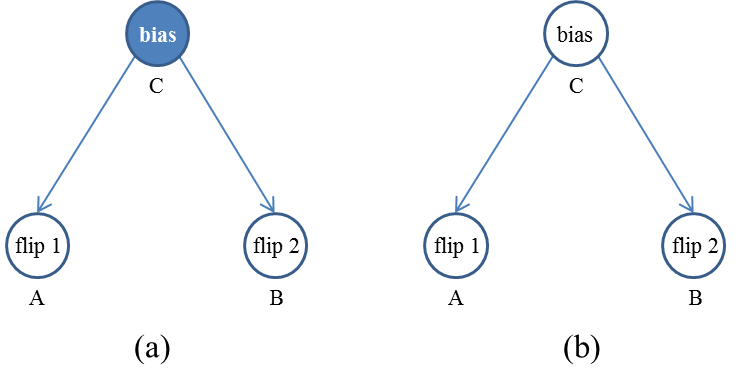
\includegraphics[width=0.45\textwidth]{BayesianModel.png}
\end{center}
\vspace{-0.35em}
\caption{Conditional dependence in Bayesian Model.}
\label{fig:BN}
\end{figure}

The dependence structure in Bayesian networks can be understood using
a coin flipping example with a biased coin.  Suppose A represents the
outcome of the first coin flip, B represents that of second coin flip
and C represents the coin's bias.  Suppose we know this bias is
$P(Heads) = 0.7$, then both the flips are independent --- irrespective
of the first flip the second flip gives \textit{heads} with
probability $0.7$. If the bias is unknown, however, then the value of
$B$ is conditionally dependent on $A$.  Thus, knowing that $A = Heads$
increases belief that the bias is towards \textit{Heads} -- that $C >
0.5$.  Therefore, the probability that the second coin flip gives
\textit{Heads} (\ie $B = Heads$) increases.

\SYSTEMLEO{} exploits this conditional dependence in the presence of
hidden, or unobserved, random variables.  \SYSTEMLEO{} models the
performance and power consumption of every system configuration as a
random variable drawn from a Gaussian probability distribution with
unknown mean and standard deviation.  \emph{Therefore, previously
  observed applications will condition \SYSTEMLEO{}'s estimations of the
  performance and power for new, unobserved applications.}  \PUNT{This
conditional dependence is the key mechanism by which \SYSTEMLEO{} quickly
realizes that \texttt{Kmeans} (from the example section) does not scale past 8
cores.}

\begin{figure*}
\begin{center}
 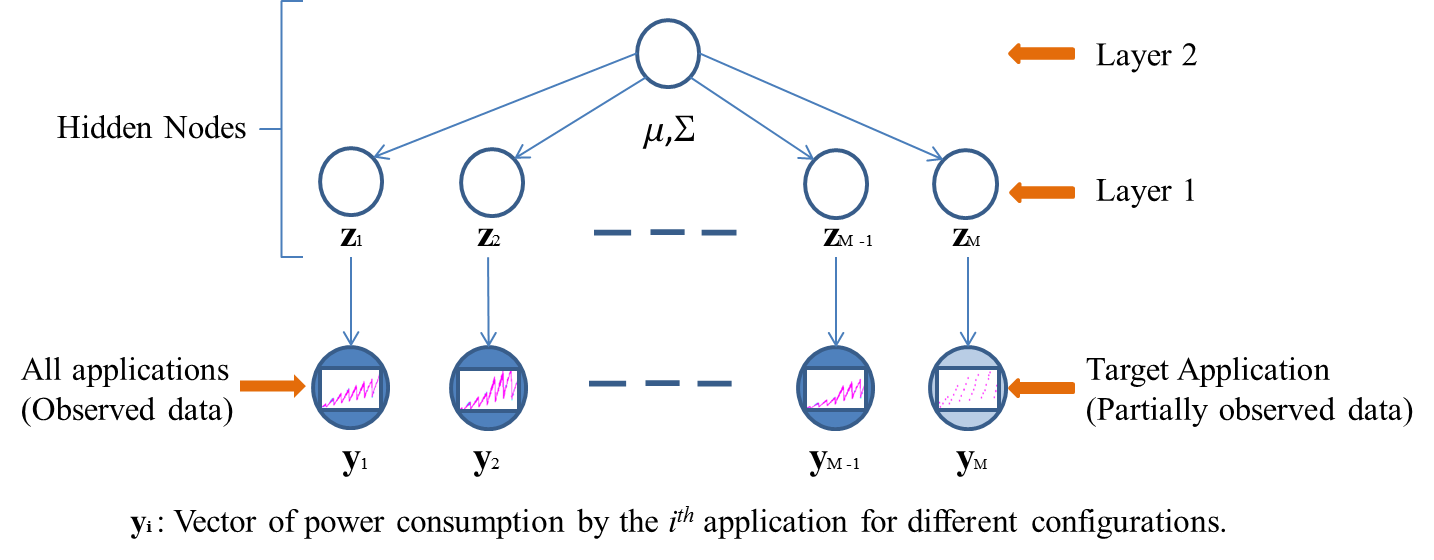
\includegraphics[width=0.85\textwidth]{HierarchicalModel.png}
\vspace{-0.35em}
\caption{Hierarchical Bayesian Model.}
\label{fig:HBN}
\end{center}
\end{figure*}


\subsection{ Hierarchical Bayesian Model}
Hierarchical Bayesian Models are slightly more complex Bayesian
networks, usually with more than one layer of hidden nodes
representing unobserved variables. \SYSTEMLEO{} utilizes these hidden
nodes to improve its estimates for a new application using prior
observations from other applications. The intuition is that
\textit{knowing about one application should help in producing better predictors for other applications}. In our examples, learning about one
biased coin flip should tell us something about another.  Similarly,
learning about another application that scales up to 8 cores should
tell us something about Kmeans. \SYSTEMLEO{} utilizes this conditional
dependence in the problem of performance and power prediction for an
application using other applications. \SYSTEMLEO{}'s model is explained
in the figure \figref{fig:HBN},

Suppose we have $n = |\mathcal{C}|$ configurations in our system.  We
have a \textit{target application} whose energy we wish to minimize,
while meeting a performance requirement (as in \eqref{eq:controller}).
Additionally, we have a set of $M-1$ applications whose performance
and power are known (as they have been measured offline).

%\TODO{Consider replacing y with p to be consistent with prior section.}
  We will illustrate how \SYSTEMLEO{} estimates power as a
function of system configuration. The identical process is used to
estimate performance.  Let the vector $\y_i \in \R^{n}$ represent the
power estimate of application $i$ in all $n$ configurations of the
system; \ie the $c$th component of $\y_i$ is the power for application
$i$ in configuration $c$ (or $\y_i[c] = p_c$).  Also, let $\{\y_i\}_{i =1}^M$ be the shorthand for the power estimates for all applications.  Without loss of generality, we assume that the first $M-1$
columns, \ie $\{\y_i\}_{i =1}^{M-1}$ represent the data for those
applications whose power consumption is known (this data is collected
offline).  The $M$th column, $\y_M$ represents the power consumption
for the new, unknown application.  We have some small number of
observations for this application.  Specifically, for the $M$th application we have observed
configurations belonging to the set $\Omega_M$ where $|\Omega_M| \ll
n$; \ie we have a very small number of observations for this
application.  Our objective is to estimate the power for application
$M$ for all configurations that we have not observed.
The model is described in terms of statistical equations below,

\begin{equation}
\begin{aligned}
\y_i \vert \z_i  &\sim N( \z_i, \sigma^2 \I),\\
\z_i \vert \mu,\Sigma &\sim N(\mu, \Sigma),\\
\mu, \Sigma &\sim N(\mu_0,\Sigma / \pi)IW(\Sigma | \nu, \Psi),
\end{aligned}
\label{eq:HBN}
\end{equation}

where $\y_i \in \R^n, \;
\z_i \in \R^n, \;
\mu \in \R^{n}, \;
\Sigma \in \R^{n\times n}$. It describes that the power (denoted by $\y_i$) for each of the $i^{th}$ application,  is drawn from multivariate-Gaussian distribution with mean $\z_i$ and a diagonal covariance matrix $\sigma^2\I$. Similarly, $\z_i$ is from multivariate-Gaussian distribution with mean $\mu$ and covariance $\Sigma$. And, $\mu$ and $\Sigma$ are jointly drawn from normal-inverse-Wishart distribution with parameters  $\mu_0, \pi,\Psi, \nu$. The parameters for our model are $\mu,\Sigma$, whereas,  $\mu_0, \pi,\Psi, \nu$ are the hyper-parameters, which we set as $\mu_0 = 0, \pi = 1,\Psi = \I, \nu = 1$.

The first layer in this model as described in \figref{fig:HBN}, is the filtration layer and accounts for the measurement error for each application. Interestingly, even if we have just a single measurement of each configuration for each application, this layer plays a crucial role as it creates a shrinkage effect. The shrinkage effect penalizes large variations in the application and essentially help in reducing the risk of the model (See \cite{efron1975data} for  shrinkage effect and \cite{morris1983parametric} for shrinkage in hierarchical models). The second layer on the other hand binds the variable $\z_i$ for each application and
enforces that they are drawn from the same distribution with unknown
mean and covariance. We work with a normal-inverse-Wishart distribution as described in \cite{gelman2013bayesian} as our hyper prior on $\mu, \Sigma$, since this distribution is the conjugate prior for a multivariate Gaussian distribution.
Thus, we essentially have a normal means model at
the first level of our hierarchy for each of the different apps and we
have a Gaussian prior on the parameter of this model. Now, if the mean
$\mu$, covariance $\Sigma$ and noise $\sigma$ were known, $\y_i$ are
conditionally independent given these parameters. Since they are
unknown we have introduced a dependence amongst all the $\y_i$s. This
is a similar situation to our coin flipping example in \figref{fig:BN}, where the value of one coin influences our prediction
about the other coin. $\Sigma$ captures the correlation between different configurations as depicted in \figref{fig:Sigma}.



\begin{comment}
\vspace{-0.35em}
\begin{algorithm}[h]
\caption{\SYSTEMLEO{} algorithm for power estimation}
\begin{algorithmic}[1]
\REQUIRE M $\leftarrow$ Number of applications, n $\leftarrow$ Number of configurations. $\{\y_i\}_{i = 1}^{M}$ $\leftarrow$ Power measurements for M applications. $\Omega_i$  $\leftarrow$ Known indices in $\y_i$. $\Omega$  $\leftarrow$ $ \{\Omega_i\}_{i = 1}^{M}$, $\epsilon \leftarrow \text{Tolerance to control convergence}$.

\STATE Construct indicator matrix $L \in \R^{n x M}$ from $\Omega$. $L_i(j) = 1$ if $j \in \Omega_i$, $L_i(j) = 0$ otherwise.
\STATE Initialize $\theta = \mu, \Sigma,\sigma$ and likelihood $\hat{\textit{L}}_0, \epsilon$.
\STATE Set $\hat{\textit{L}}  = 2\hat{\textit{L}}_0 $.
\REPEAT
	\STATE Expectation step: Compute $C_i$ and $\hat{\z}_i$ using \eqref{eq:conditionals},
	\STATE Maximization step: Compute $\theta = (\mu, \Sigma, \sigma)$ using \eqref{eq:maximization},
	\STATE Calculate likelihood $\hat{\textit{L}}  = \textit{L} \left(\theta  \vert \{ \phi(y_i ) \}^M, \{ \hat{\z}_i\}^M \right)$ using Equation \eqref{eq:likelihood}.
	\STATE Set $\hat{\textit{L}}  = \hat{\textit{L}}_0  $.
\UNTIL{$\frac{\|  \hat{\textit{L}} - \hat{\textit{L}}_0  \|}{\hat{\textit{L}}_0 } > \epsilon$}
\STATE $ \hat{\y}_M = \hat{\z}_M$
\RETURN $ \hat{\y}_M$.
\end{algorithmic}
\label{alg:LEO}
\end{algorithm}
\end{comment}
We use $\theta = \{\mu, \Sigma, \sigma\}$ to denote the unknown
parameters in the model. It can be shown that $\y_M$ is Gaussian given
$\theta$ (See \cite{yu2005learning}). %\TODO{Never say ``it can be shown.''  Always either show it   or have a citation.  Then you just say, $\y_M$ is Gaussian givenm  $\theta$ and cite or refer to your prior derivation.}.
 Thus, the problem boils down to estimating $\theta$.  Maximum-likelihood
estimators are the set of values of the model parameters that
maximizes the likelihood function (or the probability function of the
observed outcomes given the parameter values).  Essentially, the
maximum-likelihood estimates of parameters are those values which most
agree with the model. Suppose $\phi(\y)$ is the set of the observed
entries in vector $\y$. Ideally, we would like to find the maximum
likelihood estimate of the parameter $\theta$ by maximizing the
probability of $\y_M$ conditioned on ${\phi(\y_i)}_{i = 1}^{M}$ and
then use the expectation of $\y_M$ given ${\phi(\y_i)}_{i = 1}^{M}$
and $\hat{\theta}$ and as our estimator for $\y_M$. Due to the presence of latent variables (layer 1 and layer 2 in \figref{fig:HBN}) , we do not have a closed form for $\Pr( \y_M | \{\phi(\y_i)\}_{i = 1}^{M}, \theta )$
and we have to resort to the iterative algorithms like Expectation
Maximization algorithm to solve this problem.


\subsection{Expectation Maximization Algorithm}
\label{sec:EMalg}
The EM (Expectation Maximization) algorithm is a popular approach in
statistics for optimizing over analytically intractable problems.
The EM algorithm switches between two steps: \emph{expectation} (E)
and \emph{maximization} (M) until convergence. During the E step, a
function for the expectation of the log of the likelihood is found
using the current estimate for the parameters.  In the M step, we
compute parameters maximizing the expected log-likelihood found on the
E step. These parameter estimates are then used to determine the
distribution of the latent variables in the next E step.  We have left
out some details of the algebra here, but a more detailed proof on
similar lines can be found here \cite{yu2005learning}.

As described earlier, $\Omega_i$ is the set of observed indices for
$i^{th}$ application. Let $L$ denote the indicator matrix with $L(i,j)
= 1$ if $j \in \Omega_i$
and $0$ otherwise. That is, $L(i,j) = 1$ if we have observed application $i$ in system configuration $j$.  We are using $L_i$ for $L(:,i)$ for $i^{th}$ application for shorter notation. We can write the expectation and covariance for $\z_i$ given $\theta$ as following,

\begin{equation}
\begin{aligned}
\label{eq:expectation}
 \text{Cov}(\z_i) =  \left( \frac{\diag(L_i)}{\sigma^2} +\Sigma^{-1} \right)^{-1} \;\; \text{and} \\
 \E(\z_i) = \hat{\mathbf{C}}_i \left(  \frac{\diag(L_i) \y_i}{\sigma^2} +  \Sigma^{-1} \mu  \right).
 \end{aligned}
\end{equation}

\begin{comment}
\textbf{E step}: We calculate the expected log-likelihood as,
$$Q(\theta) = \E_{\{\z_i\}^M | \{ \phi(\y_i) \}^M, \mu, \Sigma }( -\log (f ( \{ \phi(y_i )  \}^M, \{\z_i\}^M  \vert \theta)f(\mu,\Sigma)  ), $$

The log of the likelihood function is given by,
\begin{equation}
\begin{aligned}
&\textit{L} \left(\theta \vert \{ \phi(y_i ) \}^M, \{ \z_i\}^M \right)
= \log(f \left( \{ \phi(y_i ) \}^M, \{ \z_i\}^M \vert \theta \right)),\\
&=   -\frac{1}{2} \mathlarger{ \sum}_{i = 1}^M [   \z_i' \left( \frac{\diag(L_i)}{\sigma^2} + \Sigma^{-1} \right) \z_i   - 2\left( \frac{y_i' \diag(L_i)}{\sigma^2}+\mu' \Sigma^{-1}  \right)\z_i  \\
&+ \frac{y_i' \diag(L_i) y_i}{\sigma^2}  + \mu'\Sigma^{-1}\mu  ]  - \log \left((\sqrt{2\pi\sigma})^{\| L\|_F^2} (2\pi \det(\Sigma))^\frac{M}{2}\right),\\
 \end{aligned}
 \label{eq:likelihood}
\end{equation}
Thus after some algebraic manipulation we have,
\begin{equation}
\begin{aligned}
\label{eq:estep}
Q(\theta) & = \text{Const} +  \mathlarger{ \sum}_{i = 1}^M   [ \tr \left( \left( \frac{\diag(L_i)}{\sigma^2} + \Sigma^{-1} \right) (\hat{\mathbf{C}}_i + \hat{\z}_i  \hat{\z}_i') \right) \\
&-2\left( \frac{\y_i' \diag(L_i)}{\sigma^2} +\mu' \Sigma^{-1}  \right)\hat{\z}_i   + \frac{\y_i' \diag(L_i) \y_i}{\sigma^2}  \\
&+ \mu'\Sigma^{-1}\mu  + \frac{ \| L\|_F^2}{M} \log(\sigma^2) + \log(\det(\Sigma)) ] \\ &+\log(\det(\Sigma))+\pi\mu'\Sigma^{-1}\mu+\tr(\Sigma^{-1}) ,
 \end{aligned}
\end{equation}
\end{comment}

We use $\hat{\mathbf{C}}_i$ as shorthand for  $\text{Cov}(\z_i)$ and $\hat{\z}_i$ denotes  $\E(\z_i)$. Later, we maximize log-likelihood w.r.t. $\theta$ and
taking derivative w.r.t. $\Sigma,\sigma \text{ and }\mu$ and setting them to 0 gives,
\begin{equation}
\label{eq:maximization}
\begin{aligned}
&\mu = \frac{1}{M +\pi} \sum_{i = 1}^M \hat{\z}_i,  \\
&  \Sigma = \frac{1}{M+1} \left(\sum_{i = 1}^{M}\hat{\mathbf{C}}_i + (\hat{\z}_i -\mu)(\hat{\z}_i -\mu)'\right) +\pi\mu\mu' +\I,\\
& \sigma^2 = \frac{1}{\|L\|_F^2} \sum_{i = 1}^{M}  \tr\left(\diag(L_i)(\hat{\mathbf{C}}_i' + (\hat{\z}_i - \y_i)(\hat{\z}_i - \y_i)' )\right),\\
 \end{aligned}
\end{equation}

\PUNT{
The estimation algorithm would repeat \eqref{} and  \eqref{} alternately until convergence.

Algorithm \ref{alg:LEO} summarizes how \SYSTEMLEO{} applies the E and M
steps to use prior observations to estimate values for unseen
configurations.

The algorithm alternates between the E step  and the M
step until convergence and the convergence criterion checks if the
relative likelihood (measured using Equation \eqref{eq:likelihood}) is
sufficiently small.
}

\SYSTEMLEO{} iterates over the E step (equation \eqref{eq:expectation})
and M step (equation \eqref{eq:maximization}) until convergence to
obtain the estimated parameters $\theta$. Then, conditioned on those
values of the parameters, \SYSTEMLEO{} sets $\y_M$ as $\E(\z_M | \theta)$
given by \eqref{eq:expectation}. \SYSTEMLEO{} uses the same algorithm to
estimate performance as well.

Given performance and power estimates, the energy minimization problem
can be solved using existing convex optimization techniques
\cite{PTRADE,ControlWare,Agilos,Heartbeats2}.  \SYSTEMLEO{} simply first
take the estimates, then finds the set of configurations that
represent Pareto-optimal performance and power tradeoffs, and finally
walks along the convex hull of this optimal tradeoff space until the
performance goal is reached.  The configuration representing this this
point in the Pareto-optimal space is the desired tradeoff.

\subsection{Example}
We illustrate how \SYSTEMLEO{} can be applied to our running example of
\texttt{Kmeans} from \Secref{sec:example}. We have 32 configurations
(hence $n=32$) corresponding to cores. We also have 24 other
applications (hence $M = 25$) with all the data for different
configurations collected offline and denoted by
$\{\y_i\}_{i=1}^{M-1}$; $\y_M$ denotes the power data for
\texttt{Kmeans}. Referring to \figref{fig:HBN}, \texttt{Kmeans} is the
final node, labeled ``Target Application,'' whereas the rest of the
applications would be the remaining nodes in any order. \SYSTEMLEO{}
estimates $\z_M$, the node above $\y_M$ in \figref{fig:HBN}, which is
an unbiased estimator for $\y_M$. \SYSTEMLEO{} collects data $\y_M$ for 6
different configurations (5, 10, $\cdots$, 30 cores). Hence, $\Omega_M
= \{5, 10, \cdots, 30 \}$ and $\y_M[j]$ is known iff $j \in \Omega_M$.
Also, $L_i$ or $L(:,i)$ is an all one vector of length $n$ if $i \neq
M$ and $L(j,i) = 1 \text{ if } j \in \Omega_M$ and $L(j,i) = 0$
otherwise.

Now, we describe the main steps of \SYSTEMLEO{}. The algorithm starts by
setting some initialization for the parameter $\theta = \{\mu, \Sigma,
\sigma\}$ and then evaluates equation \eqref{eq:expectation} for each
$i$th and later uses these values of $\hat{\z}_i$ and $\hat{C}_i$ to
evaluate equation \eqref{eq:maximization}, which is fed back to
expectation \eqref{eq:expectation} and so on. This alternating step
between equation \eqref{eq:expectation} and \eqref{eq:maximization}
runs until the algorithm converges. The algorithm uses $\hat{\z}_M$ as
the estimate of \texttt{Kmeans} power (\ie $p_c = \hat{\z}_M[c],
\forall c \in \mathcal{C}$ in equation \eqref{eq:controller}).
Similarly, \SYSTEMLEO{} estimates the performance $r_c$. After the
estimation step the linear program in equation \eqref{eq:controller}
is solved to obtain the best configuration.

\subsection{Discussion}

\begin{figure}
\begin{center}
\begin{tabular}[h]{cc}\hspace*{-15pt}
	 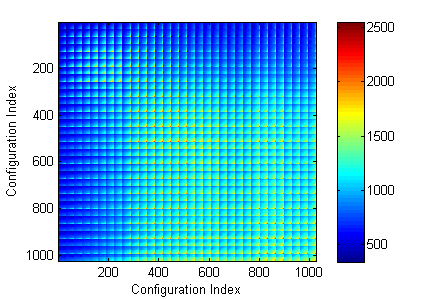
\includegraphics[width=0.45\textwidth]{Sigma.png}
\end{tabular}
\end{center}
\vspace{-1.46em}
\caption{A illustrative example of covariance $\Sigma$  between different configurations, in equation \eqref{eq:HBN}}
\label{fig:Sigma}
\end{figure}

The key to \SYSTEMLEO{} is that it does not assume any parametric
function to describe how the power varies along the underlying
configuration knobs such as cores, memory controllers or speed
settings. The upside of this representation is that \SYSTEMLEO{} captures
a much wider variety of applications, whereas the downside is a higher
computational load. \SYSTEMLEO{} finds covariance in the configurations
and exploits these relationships to estimate the data for each of the
configurations (See \figref{fig:Sigma}). We want to again point out
how our modeling of the problem is markedly different from some of
the previous approaches (such as \cite{deng2012coscale}), which assume
that power and performance are convex functions of the configuration
knobs and employ algorithms similar to gradient descent to find the
optimal configuration. While such methods work well for most
applications, it may not be suitable for more complicated
applications. \emph{In contrast, \SYSTEMLEO{} assumes that there will be
  many local minima and maxima in the functions mapping system
  configuration to power and performance -- \SYSTEMLEO{} is designed to be
  robust to the presence of local extrema, but this property is achieved at a cost of
  higher computational complexity.}

We describe some of the properties of \SYSTEMLEO{}. The EM algorithm's
convergence is dependent on the initial model
\cite{wu1983convergence}.  We can initialize the algorithm randomly.
Empirically, however, we observe that the initialization of $\mu$ with
the estimates from the online or offline approaches (given in
\Secref{sec:poc}) improves \SYSTEMLEO{}'s accuracy.  Experimentally we
have observed that the algorithm converges quickly for our benchmark
sets, generally requiring 3-4 iterations to reach the desired
accuracy. We discuss the overhead of \SYSTEMLEO{} further in
\Secref{sec:experiment:overhead}. \PUNT{In our experiments we also
  normalize the applications so that they are on the same scale, it
  helps in improving the overall accuracies.}


\section{Experimental Results}
\label{sec:experiment}
\begin{figure*}
\begin{center}
 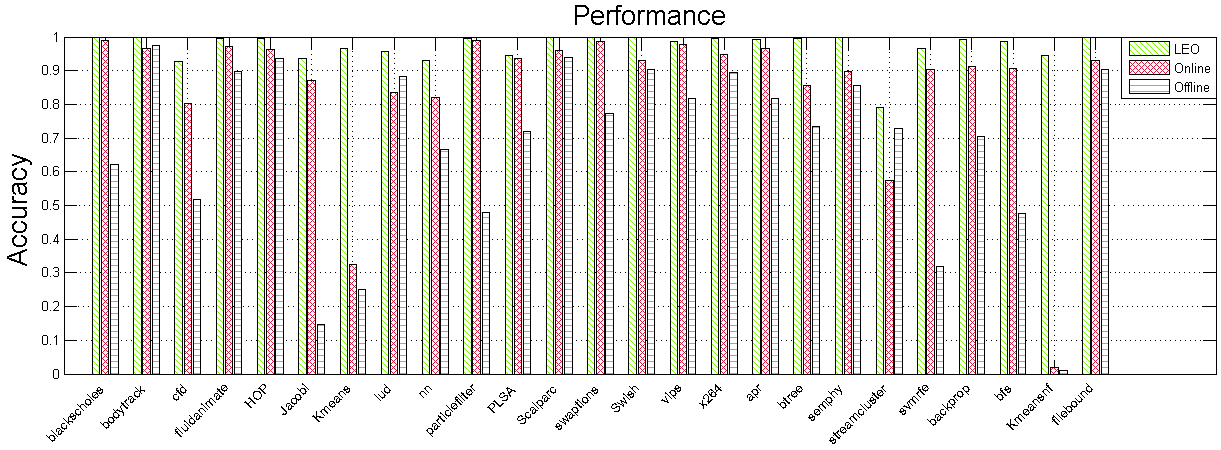
\includegraphics[width=\textwidth]{barplotPerformance.png}
 %\vspace{-7em}
 \vspace{-0.35em}
 \caption{Comparison of performance (measured as speedup) estimation
   by different techniques for various benchmarks.  \PUNT{The
     accuracies for \textit{LEO} is consistently better than
     \textit{Online} and \textit{Offline} approaches.}  On an average
   (over all benchmarks), \textit{LEO}'s accuracy is 0.97 compared to
   0.87 and 0.68 for \textit{Online} and \textit{Offline}
   respectively. The results are normalized with respect to the
   \textit{Exhaustive search} method.  }
\label{fig:barperf}
\end{center}
\end{figure*}
%\vspace{-0.35em}
\begin{figure*}
\begin{center}
 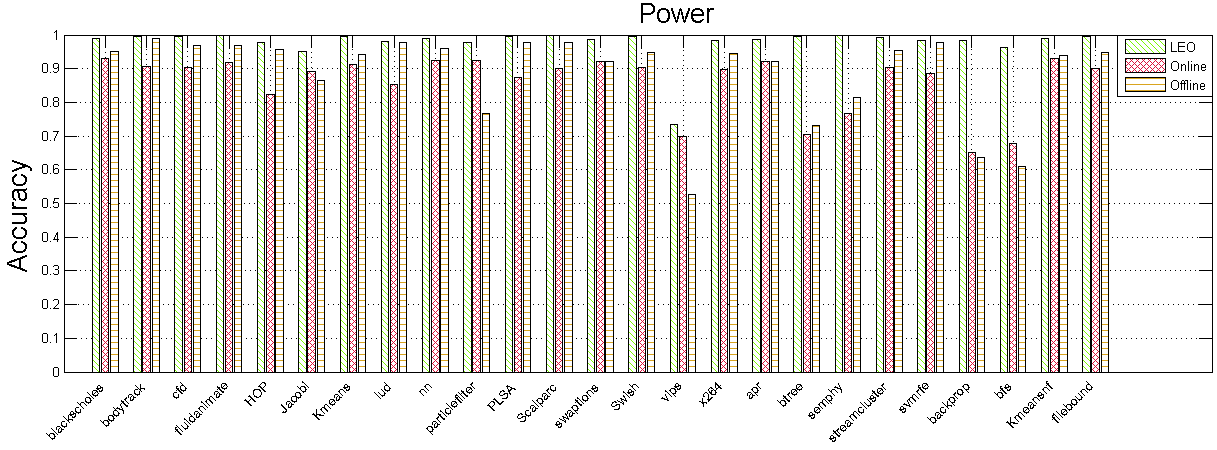
\includegraphics[width=\textwidth]{barplotPower.png}
 \vspace{-0.35em}
 \caption{Comparison of power (measured in Watts) estimation by
   different techniques for various benchmarks. \PUNT{The accuracies
     for \textit{LEO} are consistently better than the
     \textit{Offline} approach.} On an average (over all benchmarks),
   \textit{LEO}'s accuracy is 0.98 compared to 0.85 and 0.89 for
   \textit{Online} approach and \textit{Offline} approach
   respectively. Again, the results are normalized with respect to the
   \textit{Exhaustive search} method.}
\label{fig:barpower}
\end{center}
\end{figure*}
%\vspace{-0.35em}



This section evaluates \SYSTEMLEO{}'s performance and power estimates,
and its ability to use those estimates to minimize energy across a
range of performance requirements.  We begin by describing our
experimental setup and the approaches to which we compare \SYSTEMLEO{}.
We discuss \SYSTEMLEO{}'s accuracy for performance and power estimates.
We then show that \SYSTEMLEO{} provides near optimal energy savings using
these estimates.  We conclude the evaluation with a sensitivity
analysis showing how \SYSTEMLEO{} performs with respect to different
sample sizes and a measurement of \SYSTEMLEO{}'s overhead.

\subsection{Experimental Setup}
\label{sec:setup}
Our test platform is a dual-socket Linux 3.2.0 system with a
SuperMICRO X9DRL-iF motherboard and two Intel Xeon E5-2690 processors.
We use the \texttt{cpufrequtils} package to set the processor's clock
speed. These processors have eight cores, fifteen DVFS settings (from
1.2 -- 2.9 \GHz), hyper-threading, and TurboBoost.  In addition, each
chip has its own memory controller, and we use the \texttt{numactl}
library to control access to memory controllers.  In total, the system
supports 1024 user-accessible configurations, each with its own
power/performance tradeoffs\footnote{16 cores, 2 hyperthreads, 2
  memory controllers, and 16 speed settings (15 DVFS settings plus
  TurboBoost)}.  According to Intel's documentation, the thermal
design power for these processors is 135 Watts.  The system is
connected to a WattsUp meter which provides total system power
measurements at 1s intervals.  In addition, we use Intel's RAPL power
monitor to measure chip power for both sockets at finer-grain
intervals.
\begin{figure*}
\begin{center}
\begin{tabular}[t!]{ccc}\hspace*{-15pt}
	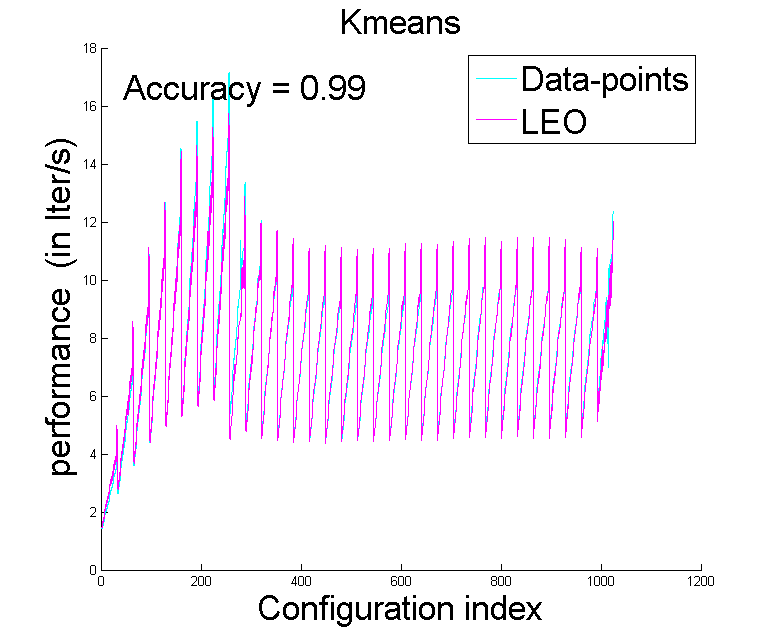
\includegraphics[width=0.3\textwidth]{performance_20_100timesmaxminYest/Kmeans.png}&
	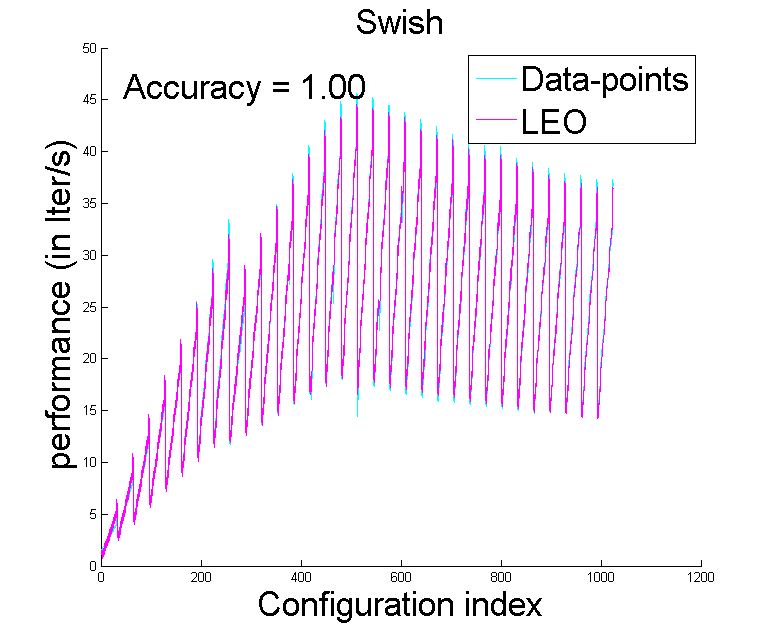
\includegraphics[width=0.3\textwidth]{performance_20_100timesmaxminYest/Swish.png}&
	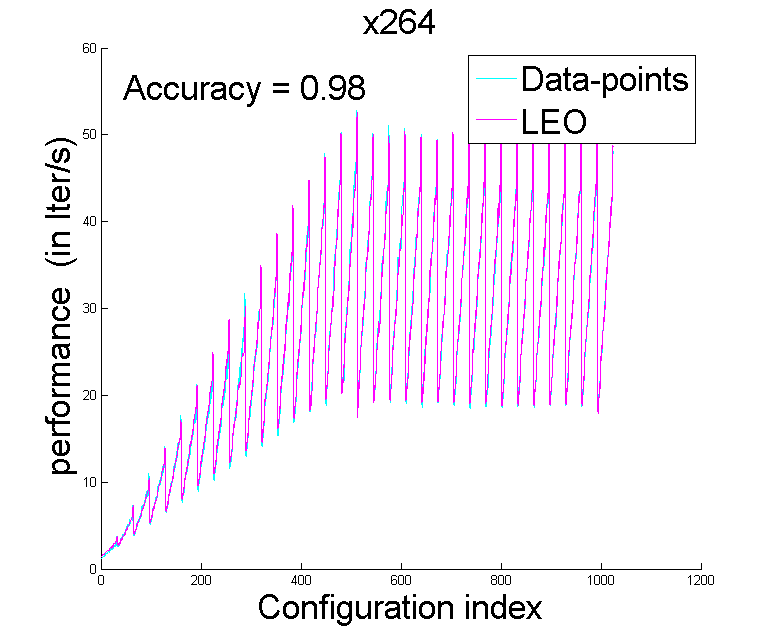
\includegraphics[width=0.3\textwidth]{performance_20_100timesmaxminYest/x264.png}\\
	{(a)} &
	{(b)} &
	{(c)}
\end{tabular}
\vspace{-0.35em}
\caption{Examples of performance estimation using \SYSTEMLEO{}.  Performance is measured as application iterations (or heartbeats) per second. (See \secref{setup}).}
\label{fig:perf}
\begin{tabular}[h]{ccc}\hspace*{-15pt}
	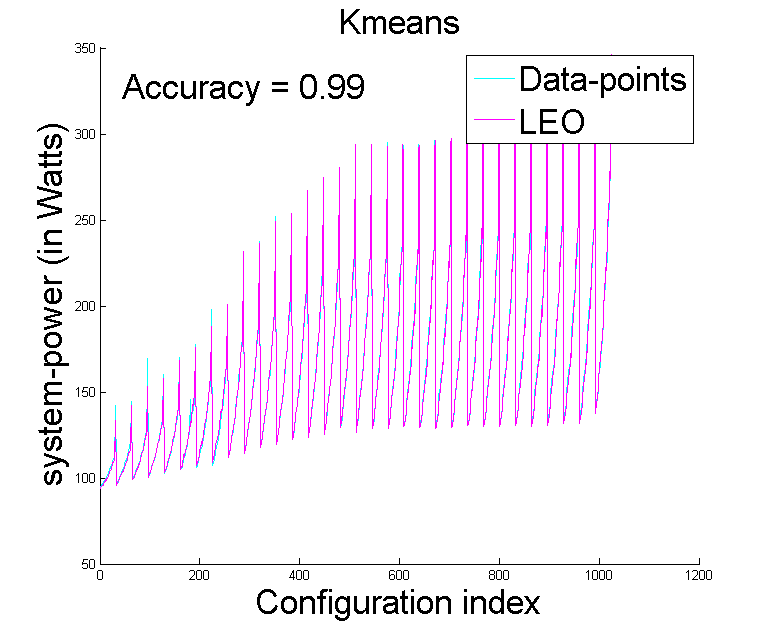
\includegraphics[width=0.3\textwidth]{system-power_20_100timesmaxminYest/Kmeans.png}&
	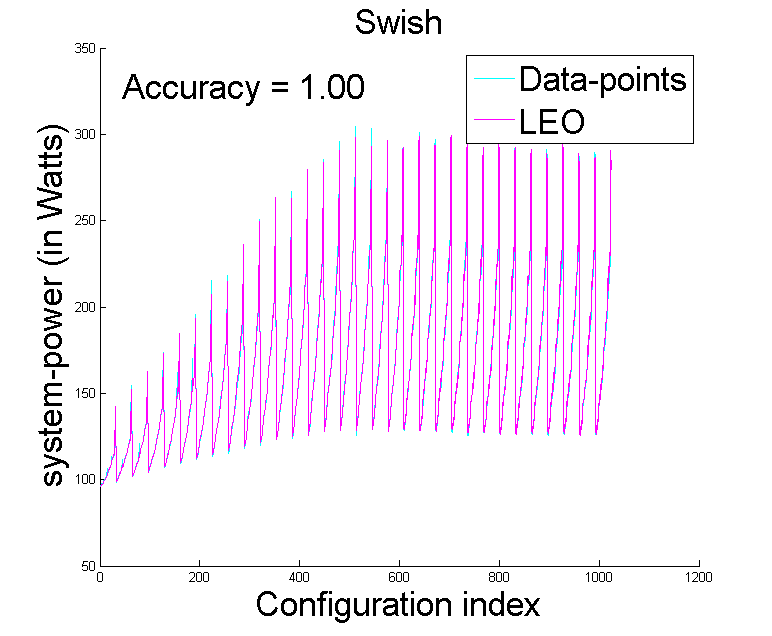
\includegraphics[width=0.3\textwidth]{system-power_20_100timesmaxminYest/Swish.png}&
	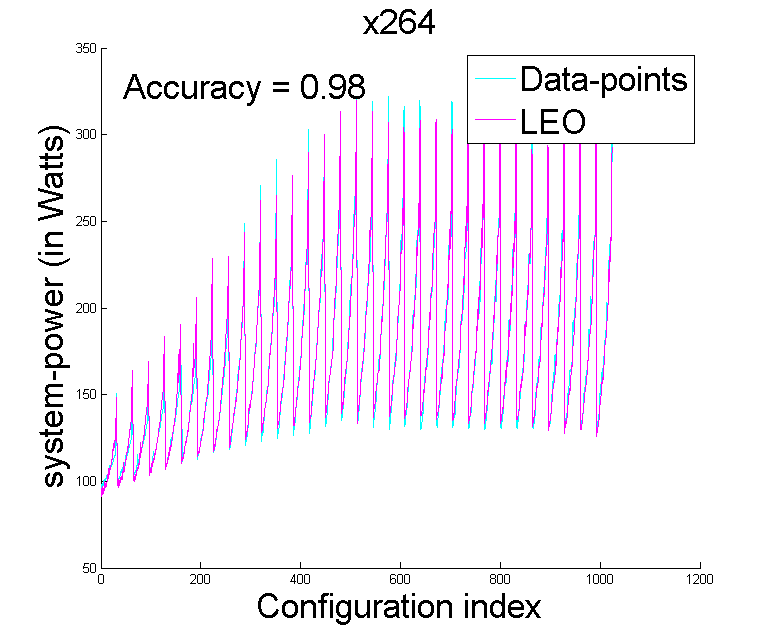
\includegraphics[width=0.3\textwidth]{system-power_20_100timesmaxminYest/x264.png}\\
	{(a)} &
	{(b)} &
	{(c)}
\end{tabular}
\vspace{-0.35em}
\caption{Examples of power estimation using \SYSTEMLEO{}. Power is
  measured as total system power. }
\label{fig:power}
\end{center}
\end{figure*}
%\vspace{-0.35em}
We use 25 benchmarks from three different suites including PARSEC
(\texttt{blackscholes}, \texttt{bodytrack}, \texttt{fluidanimate},
\texttt{swaptions}, \texttt{x264} ) \cite{parsec}, Minebench
(\texttt{ScalParC}, \texttt{apr}, \texttt{semphy}, \texttt{svmrfe},
\texttt{Kmeans}, \texttt{HOP}, \texttt{PLSA},
\texttt{non fuzzy kmeans \\* (Kmeansnf)}) \cite{minebench}, and Rodinia
(\texttt{cfd}, \texttt{nn}, \texttt{lud}, \\* \texttt{particlefilter},
\texttt{vips}, \texttt{btree}, \texttt{streamcluster},
\texttt{backprop}, \texttt{bfs}) \cite{rodinia}.  We also use a
partial differential equation solver (\texttt{jacobi}), a file
intensive benchmark (\texttt{filebound} and the \texttt{swish++}
search web-server \cite{DynamicKnobs}. These benchmarks test a range
of important multi-core applications with both compute-intensive and
i/o-intensive workloads.  All the applications run with up to 32
threads (the maximum supported in hardware on our test machine).  In
addition, all workloads are long running, taking at least 10 seconds
to complete.  This duration gives sufficient time to measure system
behavior. \PUNT{Note that various applications would work at different
  scales, hence all the data needs to be normalized so that it belongs
  to the same range.}  All applications are instrumented with the
Application Heartbeats library which provides application specific
performance feedback to \SYSTEMLEO{} \cite{Heartbeats2}. Thus
\SYSTEMLEO{} is ensured of optimizing the performance that matters to the
application.  All performance results are then estimated and measured
in terms of heartbeats/s.  In the \texttt{Kmeans} example, this metric
would represent the samples clustered per second.

To evaluate \SYSTEMLEO{} quantitatively, we measure the \emph{accuracy}
of the predicted performance and power values $\hat{\y}$ with respect
to the true data $\y$ is measured as,
\begin{equation}
\label{eq:accuracy}
\text{accuracy}(\hat{\y},\y) = \max\left(1 - \frac{\| \hat{\y}-\y \|^2_2}{\| \y - \bar{\y}\|^2_2},0\right).
\end{equation}


\subsection{Points of Comparison}
\label{sec:poc}
We evaluate \SYSTEMLEO{} in comparison to four baselines:
\begin{enumerate}
\item \textit{Race-to-idle} -- This approach allocates all resources
  to the application and once it is finished the system goes to idle.
  This strategy incurs almost no runtime overhead, but may be
  suboptimal in terms of energy, since maximum resource allocation is
  not always the best solution to the energy minimization equation
  \eqref{eq:controller}
  \cite{Carroll2013,HotPower,LeSueur11}.
\item \textit{Online} -- This strategy carries out polynomial
  multivariate regression on the observed dataset using configuration
  values (the number of cores, memory control and speed-settings) as
  predictors, and estimates the rest of the data-points based the same
  model. Then it solves the linear program given by
  \eqref{eq:controller}. This method uses only the observations and
  not the prior data.
\item \textit{Offline} -- This method takes the mean over the rest of
  the applications to estimate the power and performance of the given
  application and uses these predictions to solve for minimal energy.
  This strategy only uses prior information and we does not update
  based on runtime observations.
\item \textit{Exhaustive search} -- This brute-force approach searches
  every possible configuration to determine the true performance,
  power, and optimal energy for all applications.
\end{enumerate}

\begin{figure*}
\begin{center}
\begin{tabular}[h]{ccc}\hspace*{-15pt}
	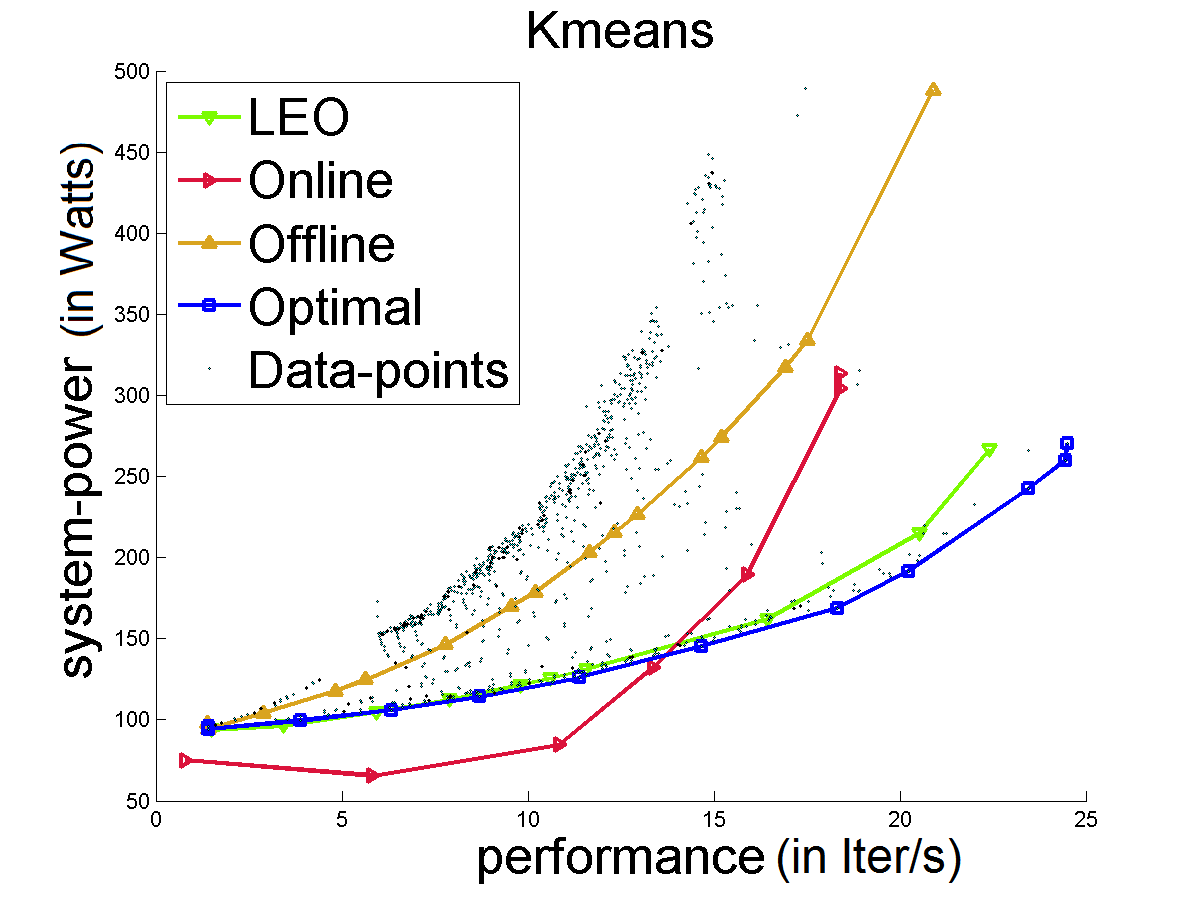
\includegraphics[width=0.3\textwidth]{combpareto_20_100timesmaxminYest/Kmeans.png}&
	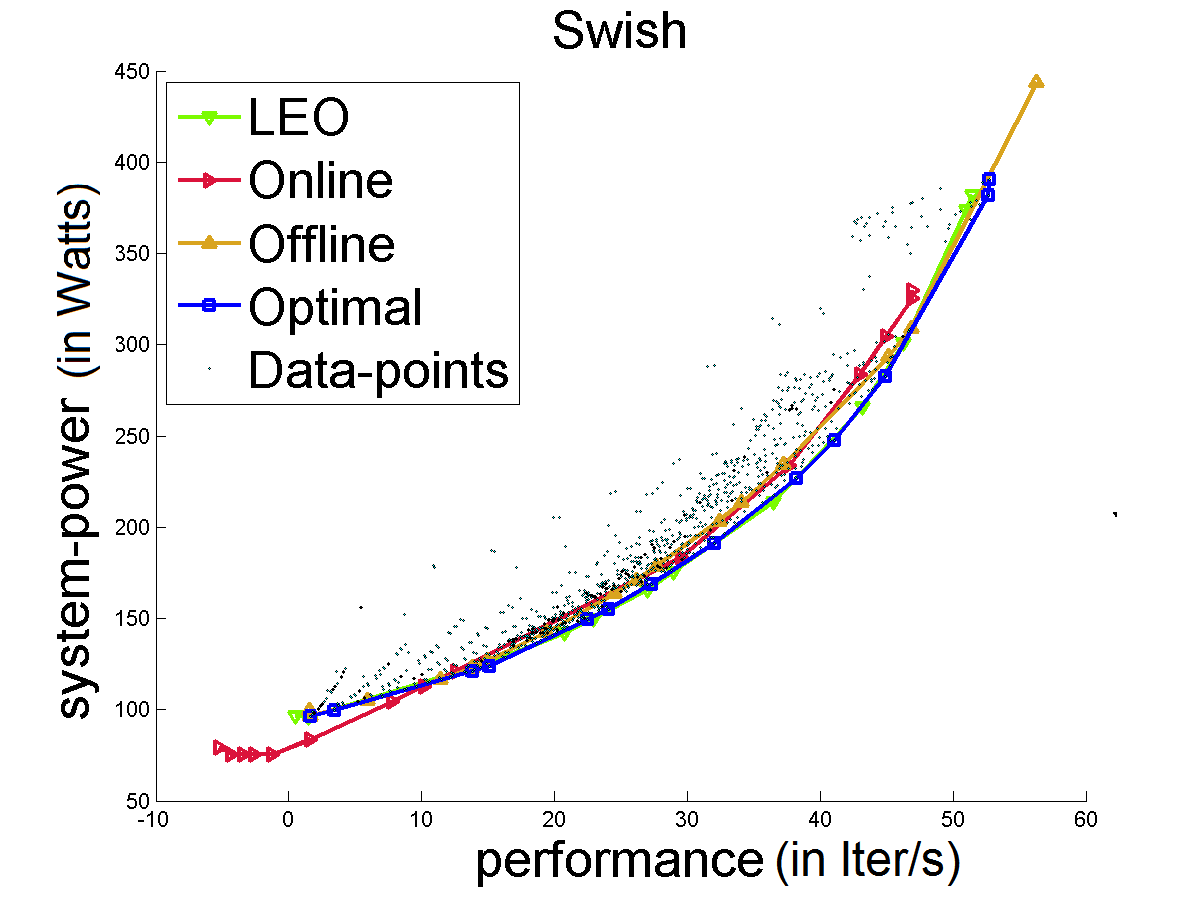
\includegraphics[width=0.3\textwidth]{combpareto_20_100timesmaxminYest/Swish.png}&
	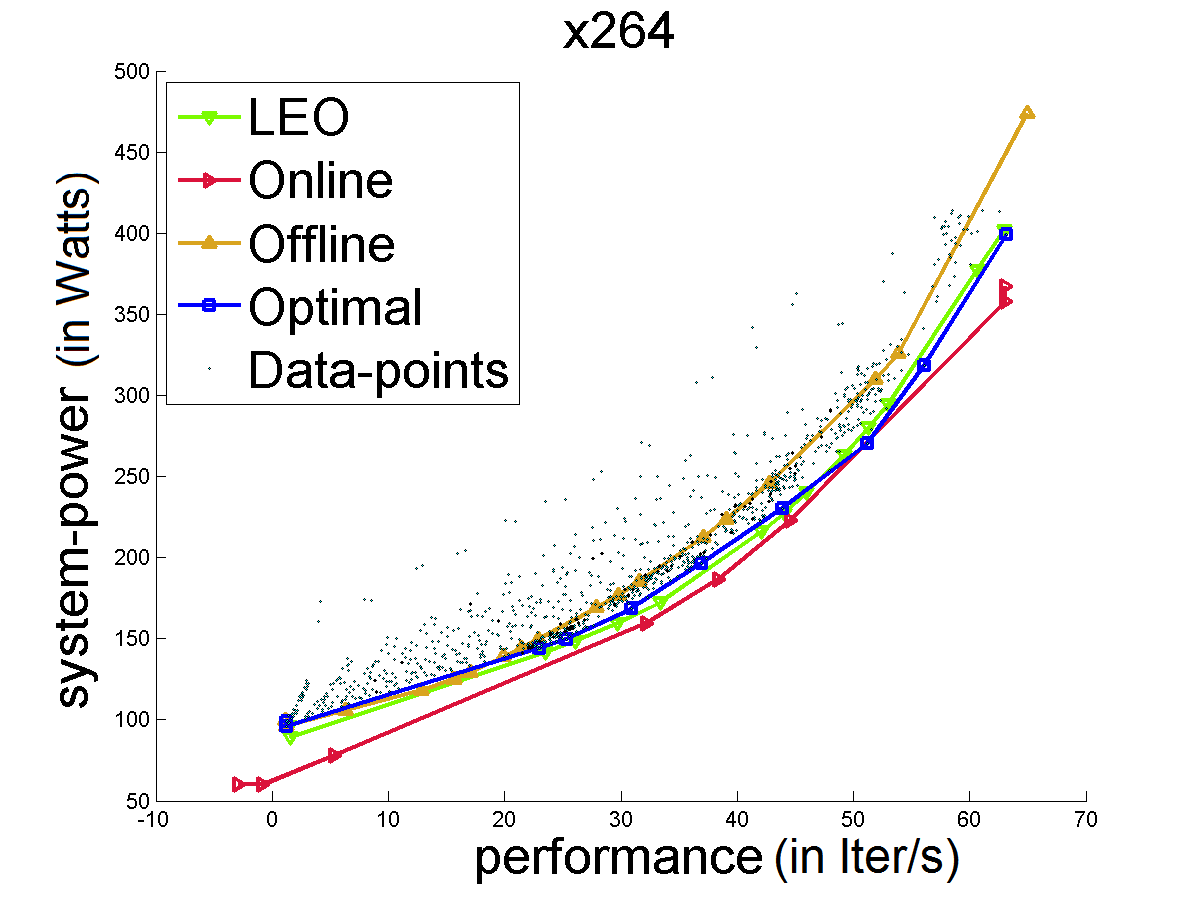
\includegraphics[width=0.3\textwidth]{combpareto_20_100timesmaxminYest/x264.png}	\\
	{(a)} &
	{(b)} &
	{(c)}
\end{tabular}
%\vspace{-0.35em}
\caption{Pareto frontier for power and performance
  estimation using different estimation algorithms. We compare estimated Pareto-optimal frontiers to the true frontier found with exhaustive search, providing insight into how LEO solves equation \eqref{eq:controller}. When the estimated curves are below optimal plots, it represents worse performance i.e. missed deadlines, whereas the estimations above the optimal waste energy.
}
\label{fig:pareto}
\begin{tabular}[h]{ccc}\hspace*{-15pt}
	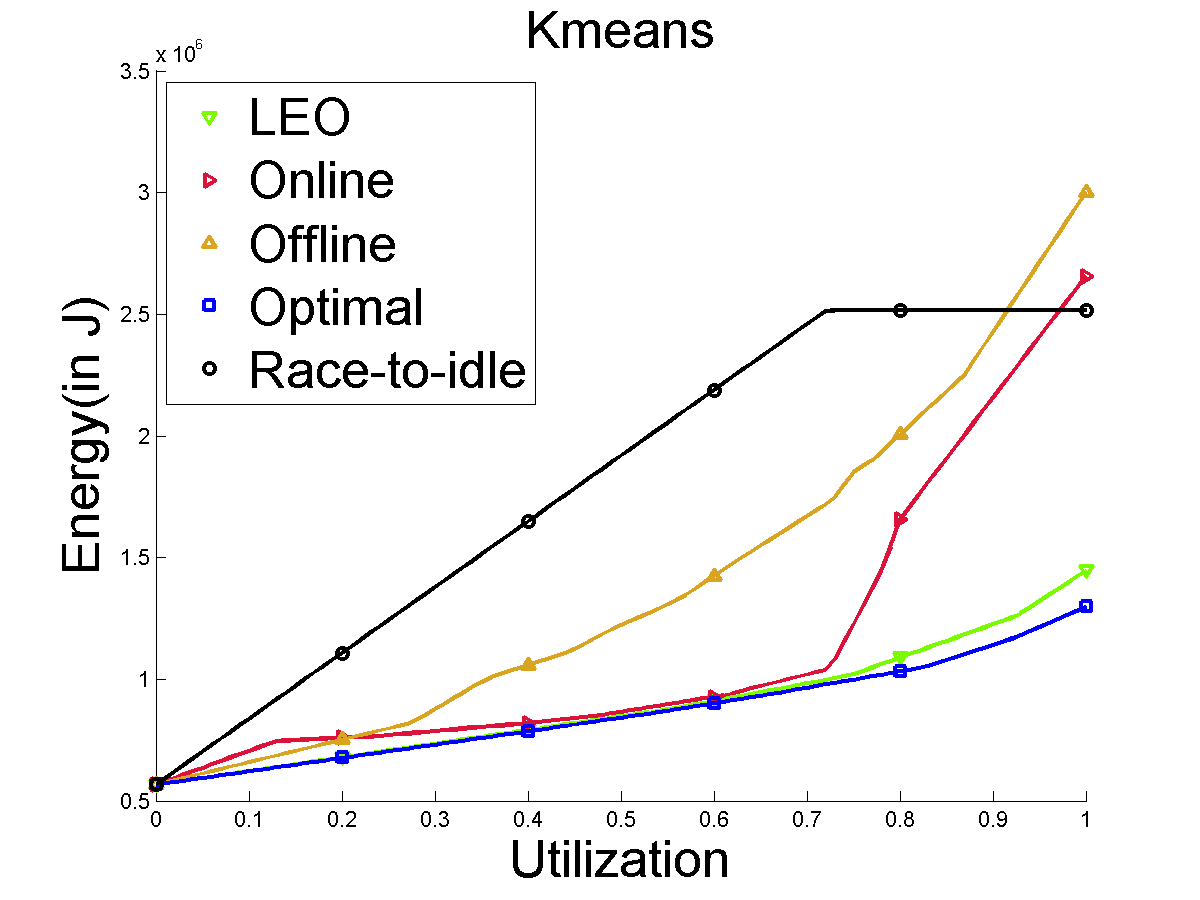
\includegraphics[width=0.3\textwidth]{LP_20_100timesmaxminYest/Kmeans.png}&
	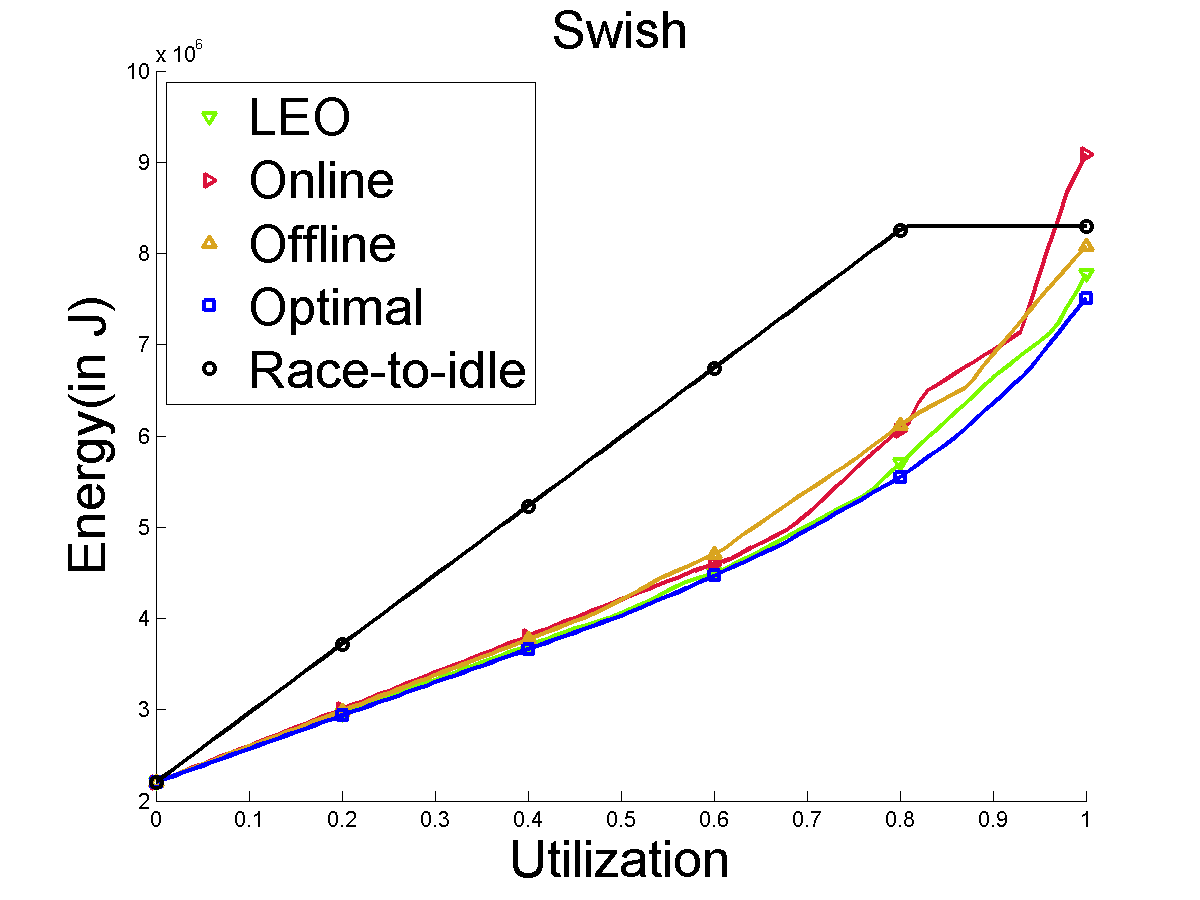
\includegraphics[width=0.3\textwidth]{LP_20_100timesmaxminYest/Swish.png}&
	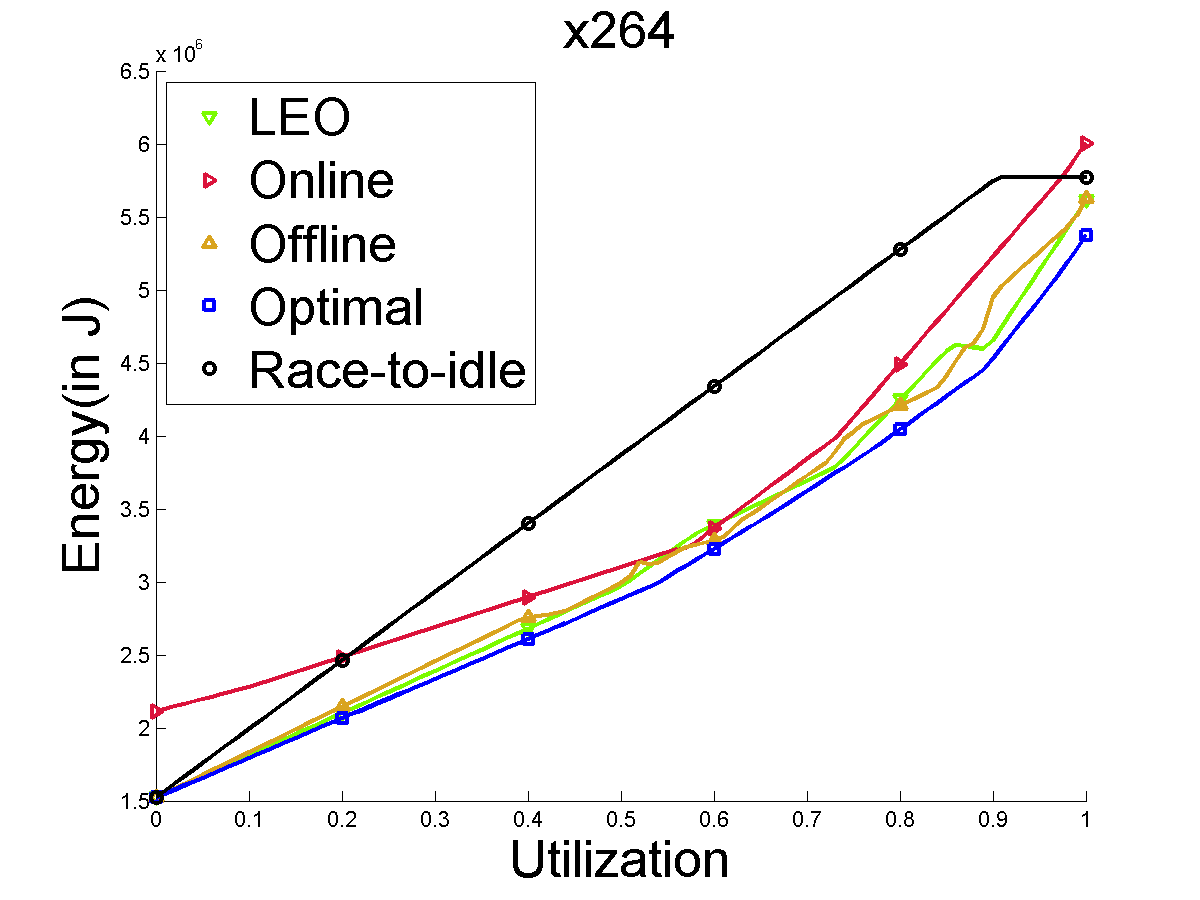
\includegraphics[width=0.3\textwidth]{LP_20_100timesmaxminYest/x264.png}\\
	{(a)} &
	{(b)} &
	{(c)}
\end{tabular}
%\vspace{-0.35em}
\caption{Energy consumption vs utilization for different
  estimation algorithms.}
\label{fig:LP}
\end{center}
\end{figure*}


\begin{figure*}
\begin{center}
 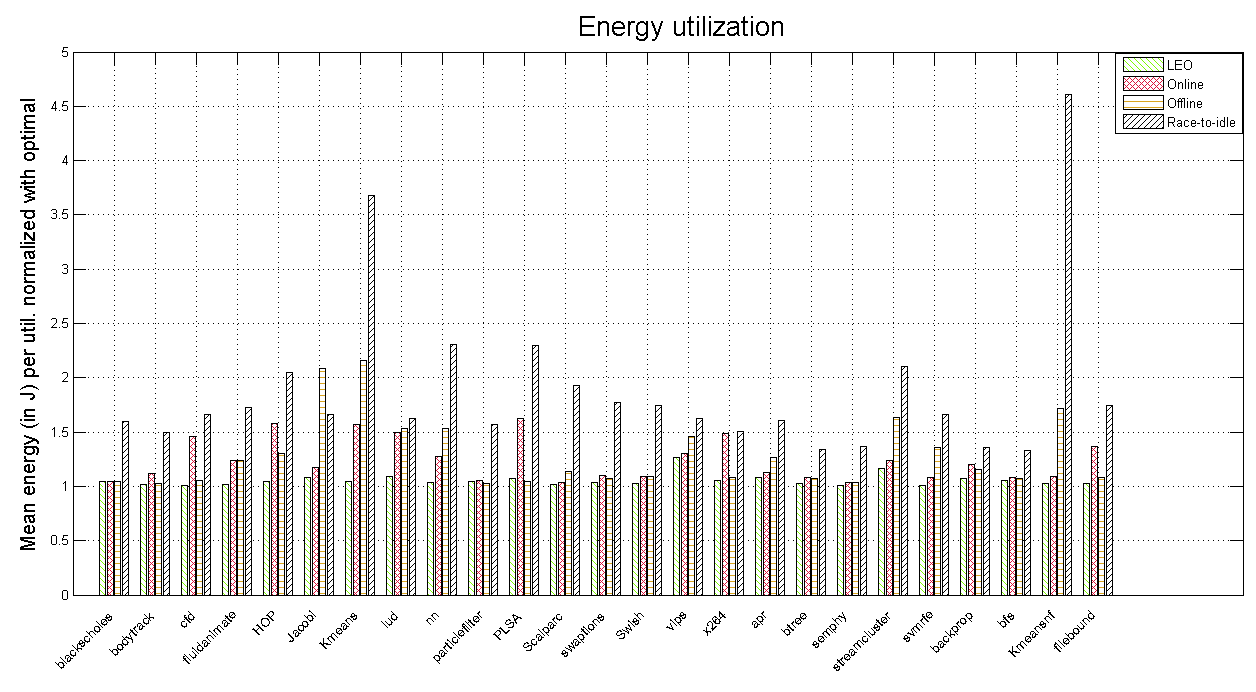
\includegraphics[width=\textwidth]{barplotEnergy.png}
 %\vspace{-0.35em}
 \caption{Comparison of average energy (normalized to
   optimal) by different estimation techniques for various benchmarks.
   \PUNT{The energy for \textit{LEO} is very close to
     \textit{Optimal}.} On an average (taken over all the benchmarks);
   \textit{LEO} consumes 6\% over optimal, as compared to the
   \textit{Online}, \textit{Offline}, and \textit{Race-to-idle}
   approaches, which respectively consume 24\%, 29\% and 90\% more
   energy than optimal. }
\label{fig:barEnergy}
\end{center}
\end{figure*}
%\vspace{-0.35em}


\subsection{Power and Performance using LEO}
\label{sec:experiment:PP}
We compare \SYSTEMLEO{}'s estimates to the \emph{online}, \emph{offline},
and exhaustive search methods described in \Secref{sec:poc}.  We deploy each of our 25 applications on our test
system and estimate performance and power.  We allow \SYSTEMLEO{} and the
online method to sample randomly select 20 configurations each. Unlike online method, which only uses these 20 samples, \SYSTEMLEO{} utilizes these 20 samples along with all the data from the other applications for the estimation purpose.  For
both \SYSTEMLEO{} and the online approach, we take the average estimates
produced over 10 separate trials to account for random variations.
The offline approach does no sampling.  The exhaustive approach
samples all 1024 configurations.

The performance and power estimation accuracies are shown in
\figref{fig:barperf} and \figref{fig:barpower}, respectively.  Each
chart shows the benchmarks on the x-axis and estimation accuracy
(computed using Equation \ref{eq:accuracy}) on the y-axis.  Unity
represents perfect accuracy.  As seen in these charts, \SYSTEMLEO{}
produces significantly higher accuracy for both performance and power.
On average -- across all benchmarks and all configurations --
\SYSTEMLEO{}'s estimations achieve $0.97$ accuracy for performance and
$0.98$ for power.  In contrast, the online approach achieves
accuracies of $0.87$ and $0.85$, while the offline approach's
accuracies are $0.68$ and $0.89$.  Even for difficult benchmarks (like
\texttt{Kmeans}), \SYSTEMLEO{} produces accurate estimations despite
sampling less than $2\%$ of the possible configuration space.

To further illustrate \SYSTEMLEO{}, we include some individual
estimations for three representative applications: \texttt{Kmeans},
\texttt{Swish}, and \texttt{x264}.  \texttt{Kmeans} is the same
application used in our example (\secref{example}), now extended to
consider all 1024 configurations of the test system.  \texttt{Swish}
is an open source search web server. \texttt{x264} is a video encoder.
All three are representative of our target applications: they are long
running and they may be launched with different performance demands.
Furthermore, all three represent some unusual trends: performance for
\texttt{Kmeans} peaks at 8 cores, for \texttt{Swish} it peaks at 16
cores, and for \texttt{x264} it is (essentially) constant after 16
cores.

Despite this behavior, \SYSTEMLEO{} produces highly accurate estimates of
performance (\figref{fig:perf}) and power (\figref{fig:power}).  Each
figure shows the configuration index on the x-axis and the predicted
performance (or power) on the y-axis.  Each chart shows both the
estimated values and the measured data points, but \SYSTEMLEO{} is so
accurate that it is hard to distinguish the two. The figures
(\figref{fig:perf} and \figref{fig:power} ) are saw-tooth in
appearance since the speed settings vary from low to high along the
\textit{Configuration index} multiple times. The saw-tooth nature of
the curves arises from two sources: (1) the extrema that naturally
arise (\eg response to cores) and (2) we have flattened a
multi-dimensional configuration space into the configuration index.
The number of memory controllers is the fastest changing component of
configuration, followed by clockspeed, followed by number of cores.
\SYSTEMLEO{} captures the peak performance configuration for all three
applications and it captures local minima and maxima.  These accurate
estimates of unusual behavior make \SYSTEMLEO{} well-suited for use in
energy minimization problems.

\subsection{Minimizing Energy}
\label{sec:experiment:LP}
%%%%%%%%%%%%%%%%%%%%%%%%% Estimation
%\vspace{-0.35em}
Our original goal, of course, is not just to estimate performance and
power, but to minimize energy for a performance (or utilization)
target.  As described in \Secref{sec:EMalg}, \SYSTEMLEO{} uses its estimates to
form the Pareto-optimal frontier of performance and power tradeoffs.
\figref{fig:pareto} shows the true convex hull and those estimated by
the \SYSTEMLEO{}, Offline and Online approaches.  Due to space
limitations, we show only the hulls for our three representative
applications: \texttt{Kmeans}, \texttt{Swish}, and \texttt{x264}.  In
these figures performance (measured as speedup) is shown on the x-axis
and system wide power consumption (in Watts) on the y-axis.  These
figures clearly show that \SYSTEMLEO{}'s more accurate estimates of power
and performance produce more accurate estimates of Pareto-optimal
tradeoffs.

To evaluate energy savings, we deploy each application with varying
performance demands.  Technically, we fix the deadline and vary the
workload $W$ from Equation \ref{eq:controller} so that $W$ $\in$
[\textit{minPerformance , maxPerformance}] for each application.  We test 100
different values for $W$ -- each representing a different utilization
demand from 1 to 100\% -- for each application.  We then use each
approach to estimate power and performance and form the estimated
convex hull and select the minimal energy configuration.

\figref{fig:LP} shows the results for our three representative
benchmarks.  Each chart shows the utilization demand on the x-axis and
the measured energy (in Joules) on the y-axis.  Each chart shows the
results for the \SYSTEMLEO{}, Online, and Offline estimators as well as
the race-to-idle approach and the true optimal energy.  As shown in
these figures, \SYSTEMLEO{} produces the lowest energy results across the
full range of different utilization targets.  \SYSTEMLEO{} is always
close to optimal and outperforms the other estimators.  Note that all
approaches do significantly better than race-to-idle. We repeat the
above experiment for all applications, then average the energy
consumption for each application across all utilization levels.  These
results are shown in \figref{fig:barEnergy}, which displays the
benchmark on the x-axis and the average energy (normalized to optimal)
on the y-axis.  On an average across all the applications, \SYSTEMLEO{}
does only 6\% worse than optimal.  In contrast, Online, Offline and
race-to-idle methods are 24\% , 29\% and 90\% worse respectively.
These results demonstrate that \SYSTEMLEO{} not only produces more
accurate estimates of performance and power, but that these estimates
produce significant -- near optimal -- energy savings.

\subsection{Sensitivity to Measured Samples}

One of the key parameters of \SYSTEMLEO{} is the number of samples it must
measure to produce an accurate estimate.  All of the above
measurements were taken with the system configured to sample 20
configurations.  In this section, we investigate the effect of the
number of configurations on the accuracy of performance and power
estimation. In \figref{fig:Sensitivity}, we show the accuracy
(averaged over all benchmarks) for performance (a) and power (b)
estimation as a function of sample size. We observe that \SYSTEMLEO{}
performs well with an even smaller sample size, whereas the Online
approach does poorly for very small sample sizes.
\begin{figure}
\begin{center}
\begin{tabular}[h]{cc}\hspace*{-15pt}
	 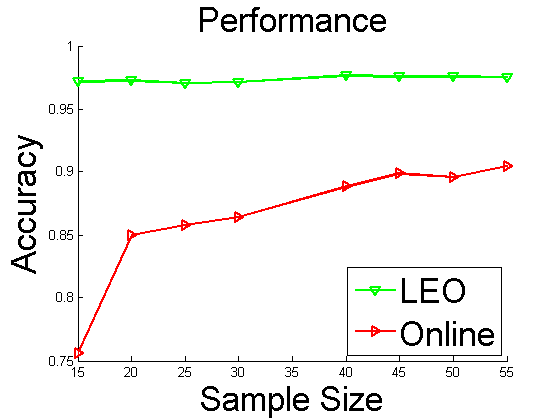
\includegraphics[width=0.5\textwidth]{AllSamplePerf.png}&
	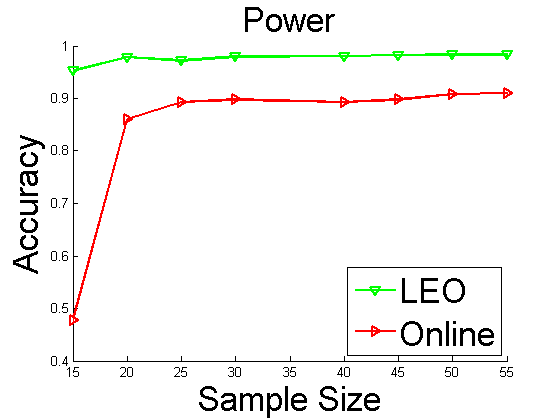
\includegraphics[width=0.5\textwidth]{AllSamplePower.png}\\
	 {(a)} &
	 {(b)}
\end{tabular}
\end{center}

\caption{Sensitivity analysis of \SYSTEMLEO{} and Online estimation. Our
  baseline method (online regression) cannot perform below 15 samples
  because the design matrix of regression model would be rank
  deficient -- effectively 0 accuracy. On the other hand, with 0
  samples, LEO behaves as the offline method and its accuracy
  increases with the sample size until it quickly reaches near optimal
  accuracy. }
\label{fig:Sensitivity}
\end{figure}
%\vspace{-0.5em}



\subsection{Reacting to Dynamic Changes}
\label{sec:controller}
%%%%%%%%%%%%%%%%%%%%%%%%%% Phases in controller



This section shows that \SYSTEMLEO{} can quickly react to changes in
application workload.  In this section we run \texttt{fluidanimate},
which renders frames, with an input that has two distinct phases.
Both phases must be completed in the same time, but the second phase
requires significantly less work.  In particular, the second phase
requires $2/3$ the resources of the first phase.  Our goal is to
demonstrate that \SYSTEMLEO{} can quickly react to phase changes and
maintain near optimal energy consumption.

\begin{figure*}
\begin{center}
\begin{tabular}[h]{cc}\hspace*{-15pt}
	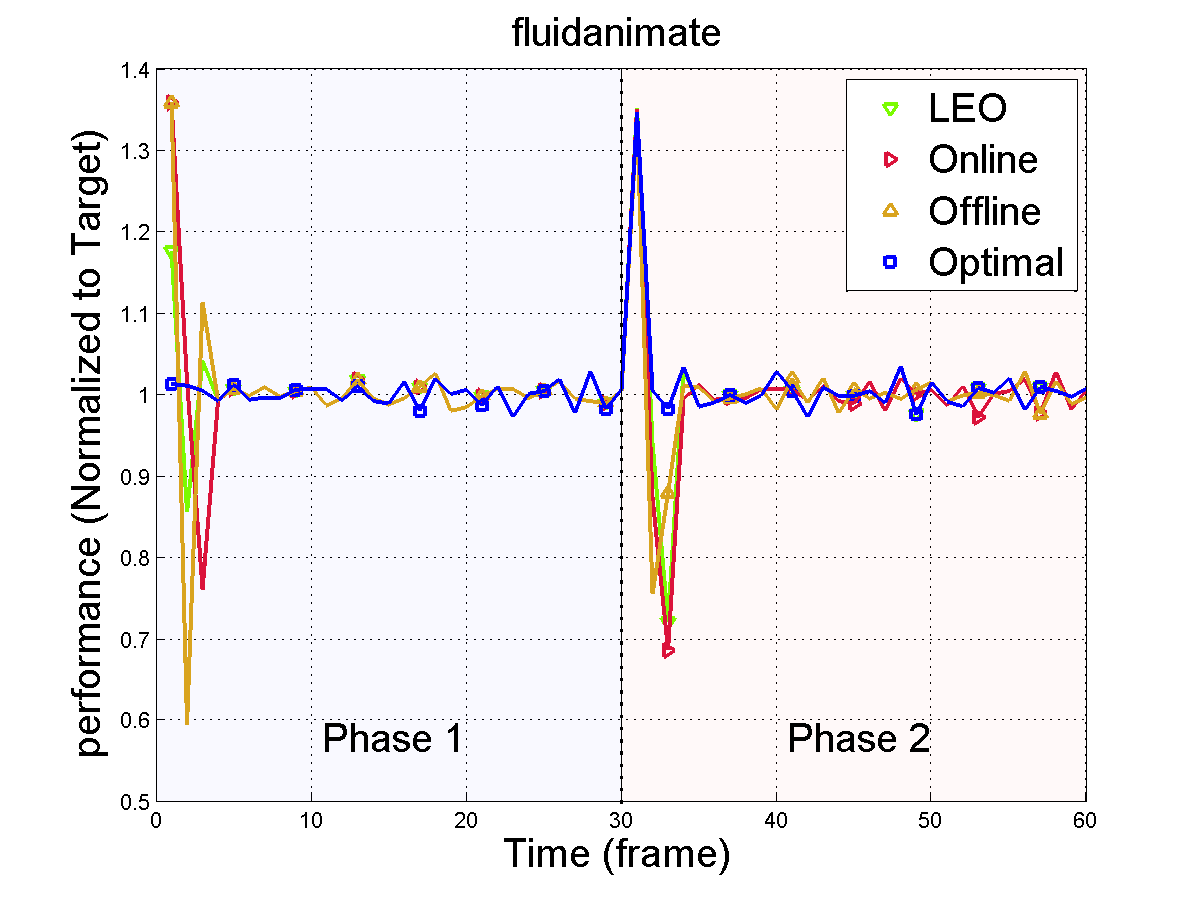
\includegraphics[width=0.5\textwidth]{Controller/fluidanimateperformance.png}&
	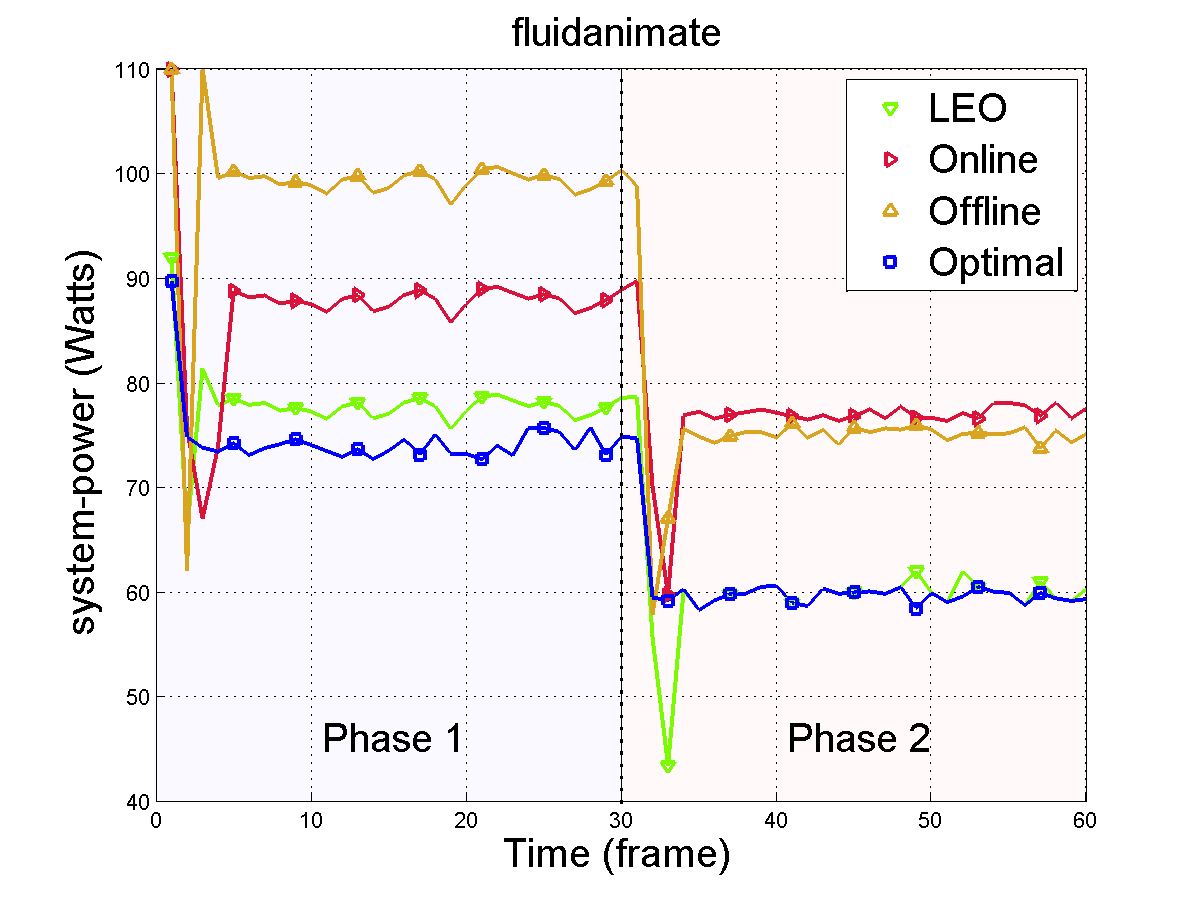
\includegraphics[width=0.5\textwidth]{Controller/fluidanimatesystem-power.png}\\
	 {(a)} &
	 {(b)}
\end{tabular}
\vspace{-0.35em}
\caption{Power and performance for \texttt{fluidanimate}
  transitioning through phases with different computational demands.}
\label{fig:phases}
\end{center}
\end{figure*}

\PUNT{
\begin{figure*}
\begin{center}
\begin{tabular}[h]{cc}\hspace*{-15pt}
	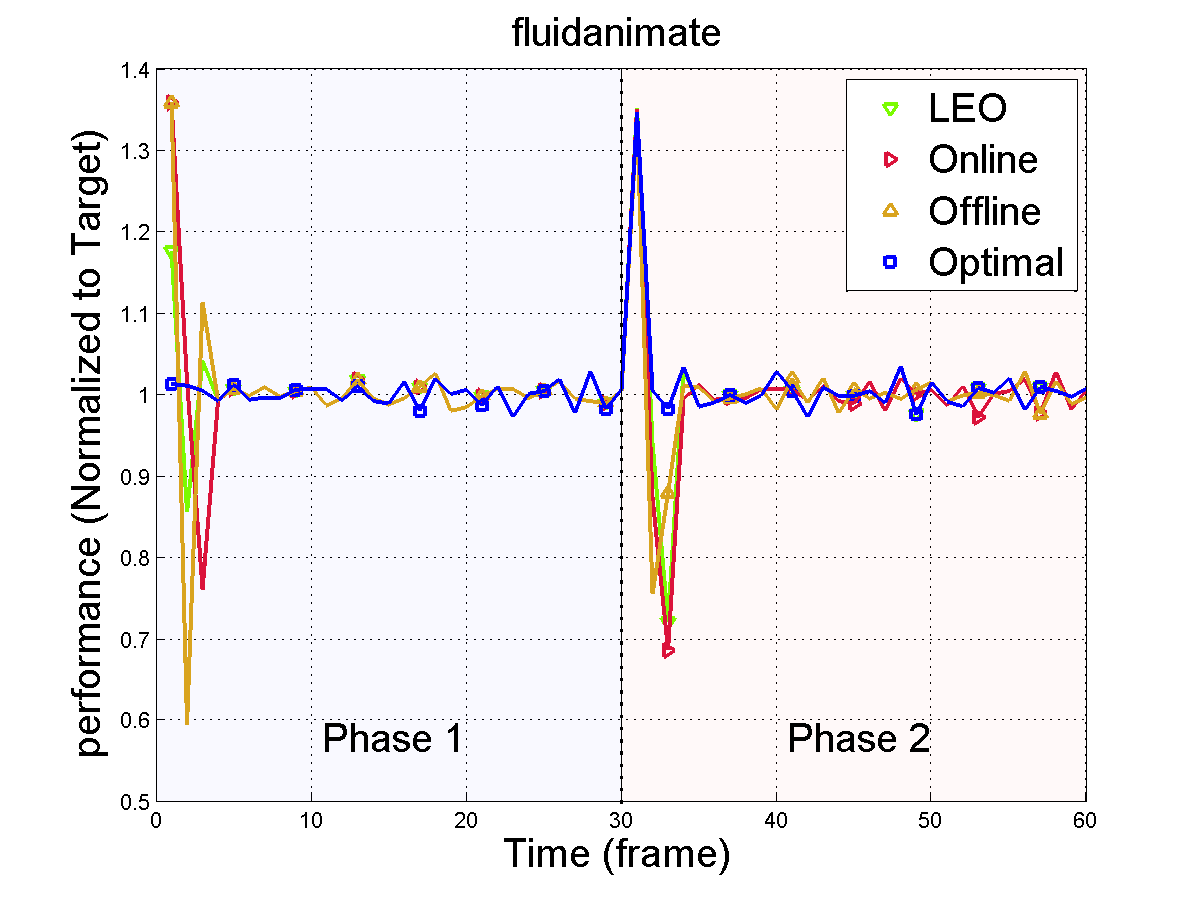
\includegraphics[width=0.45\textwidth]{Controller/fluidanimateperformance.png}&
	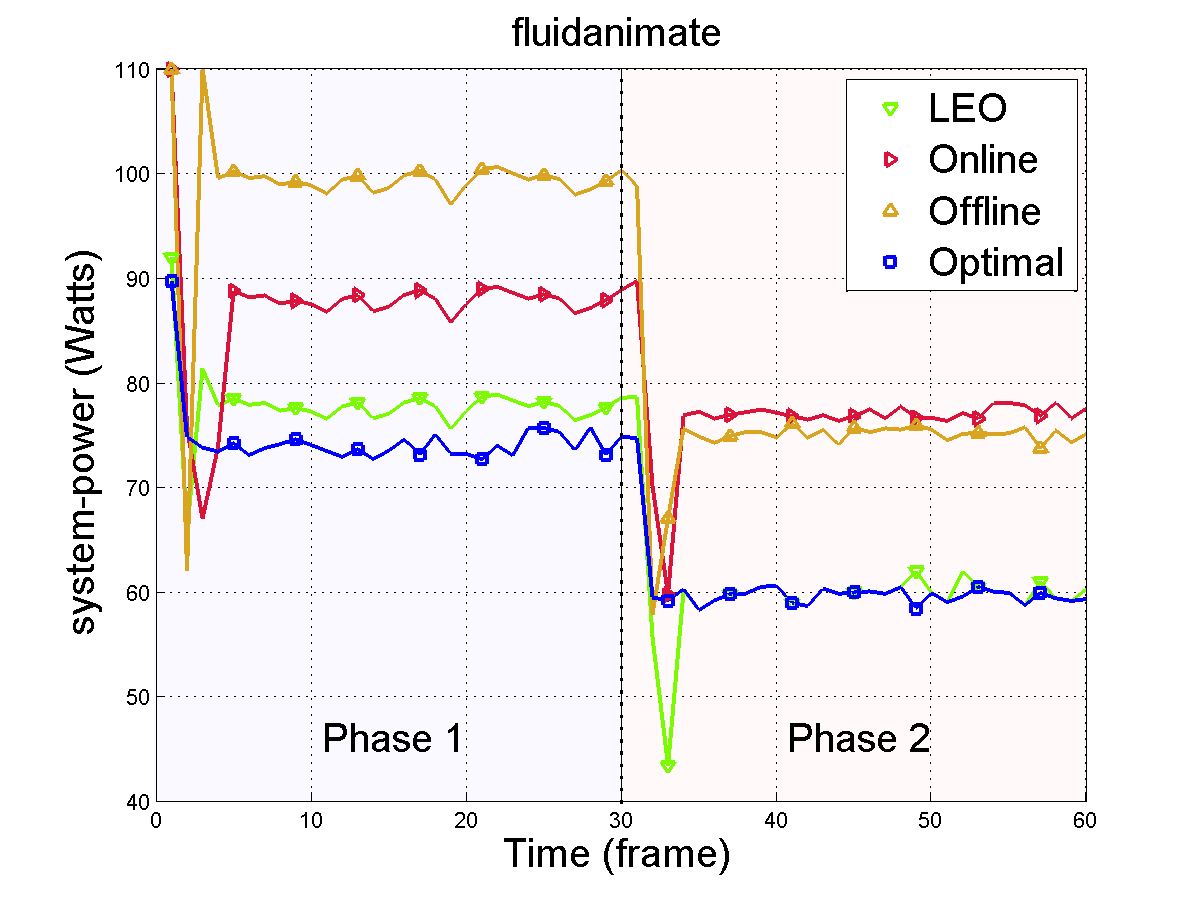
\includegraphics[width=0.45\textwidth]{Controller/fluidanimatesystem-power.png}
\end{tabular}
\vspace{-0.35em}
\caption{Power and performance for \texttt{fluidanimate}
  transitioning through phases with different computational demands.}
\label{fig:phases}
\end{center}
\end{figure*}

\begin{figure*}[t!]
    \centering
    \begin{subfigure}
        \centering
        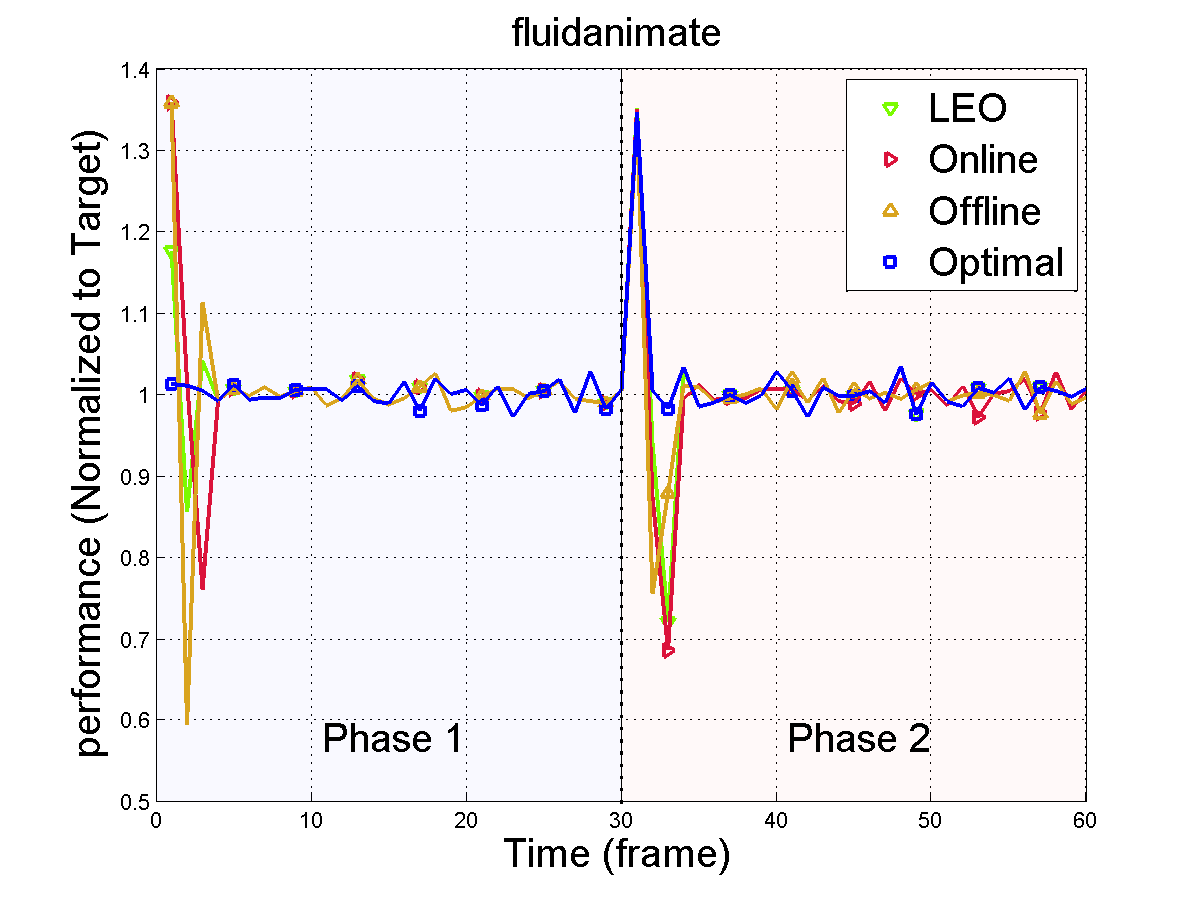
\includegraphics{Controller/fluidanimateperformance.png}
        \caption{(a)}
    \end{subfigure}%
    ~
    \begin{subfigure}
        \centering
        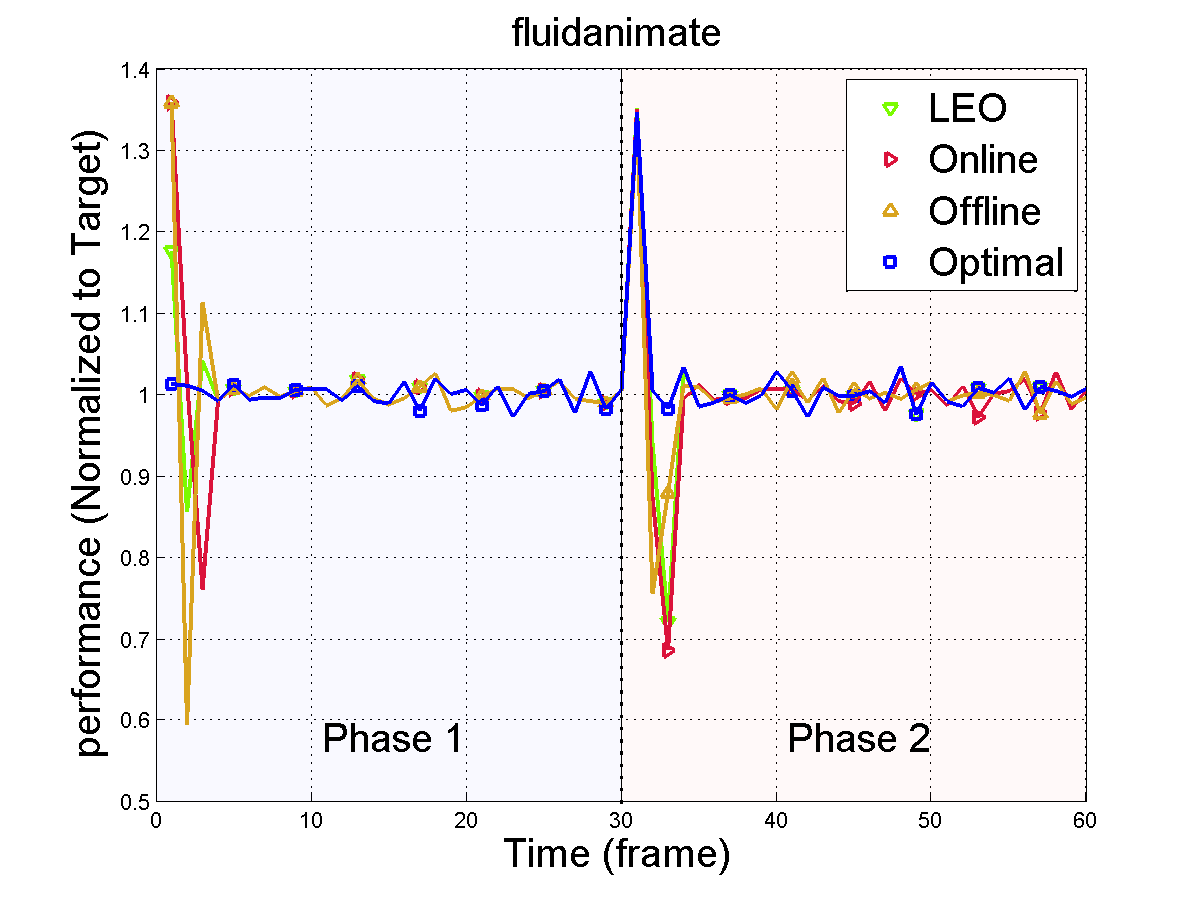
\includegraphics{Controller/fluidanimateperformance.png}
        \caption{(b)}
    \end{subfigure}
    \caption{Power and performance for \texttt{fluidanimate}
      transitioning through phases with different computational demands.}
\end{figure*}

}

\PUNT{
\begin{figure*}[t!]
    \centering
    \begin{subfigure}
        \centering
        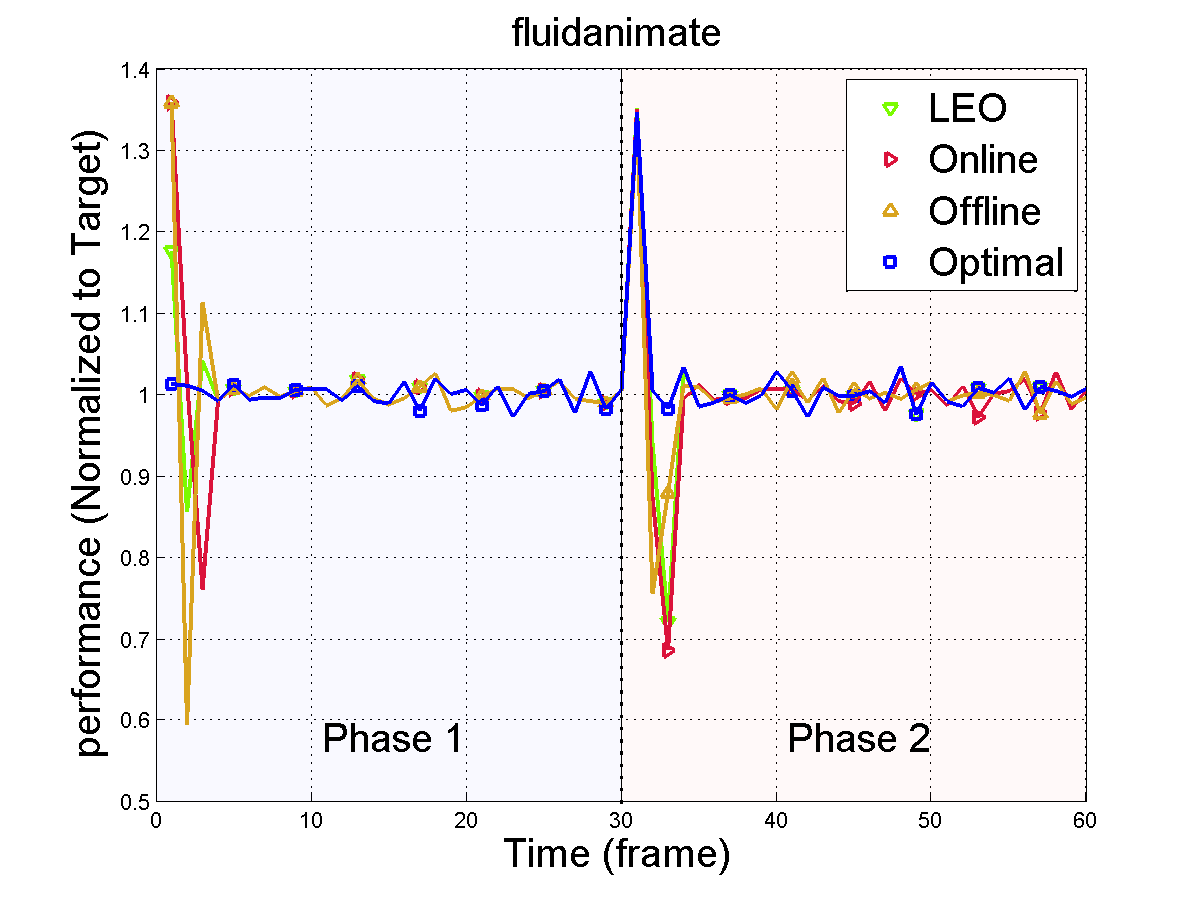
\includegraphics{Controller/fluidanimateperformance.png}
    \end{subfigure}%
    \begin{subfigure}
        \centering
        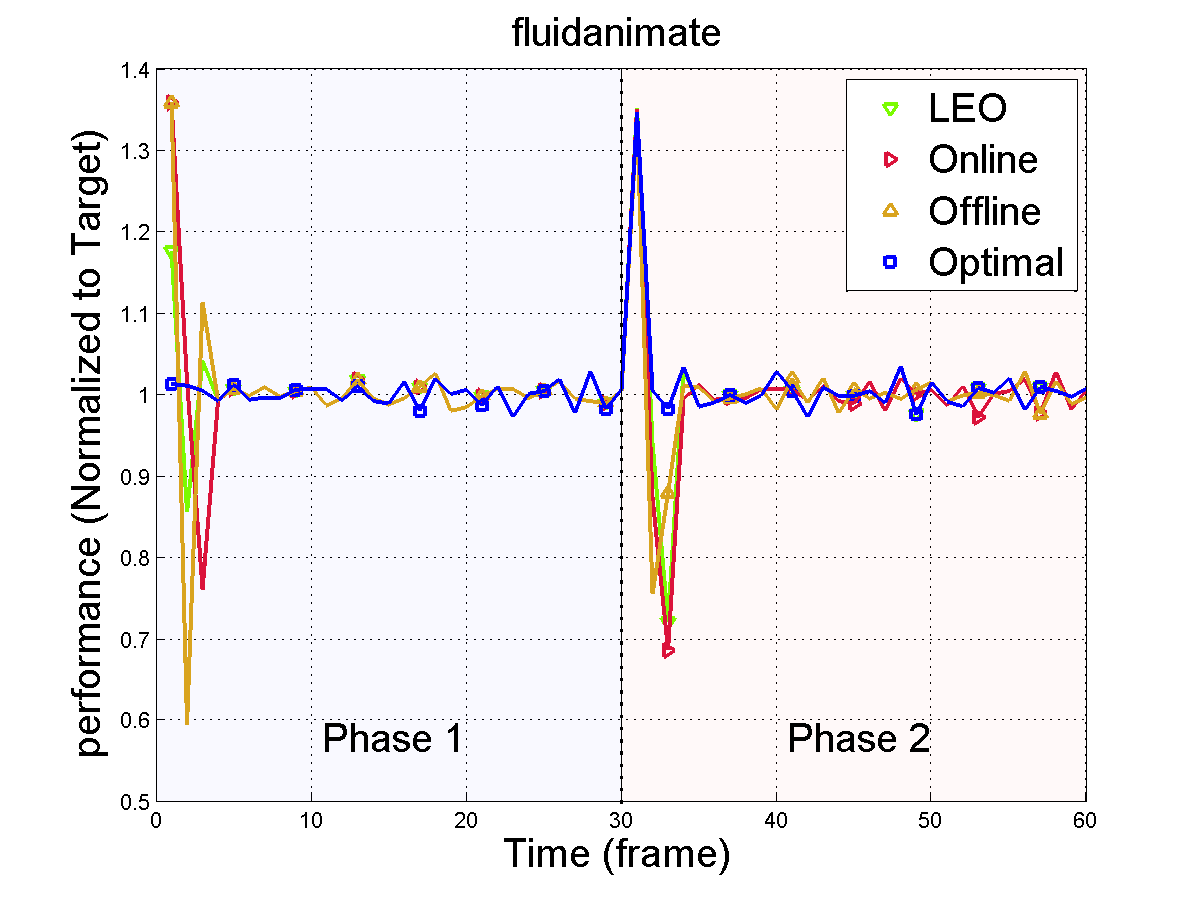
\includegraphics{Controller/fluidanimateperformance.png}
    \end{subfigure}
    \caption{Power and performance for \texttt{fluidanimate}
      transitioning through phases with different computational demands.}
\end{figure*}
}

%\vspace{-1em}

%The summarize the energy consumption in the following table.
%\vspace{-0.75em}
\begin{table}[ht]
  \caption{Relative energy consumption by various algorithms with respect to optimal.}
\centering % used for centering table
\begin{tabular}{c c c c} % centered columns (4 columns)
\hline\hline %inserts double horizontal lines
Algorithm & Phase\#1 & Phase\#2 & Overall \\ [0.5ex] % inserts table %heading
\hline % inserts single horizontal line
\text{LEO} & 1.045 & 1.005 & 1.028 \\ % inserting body of the table
\text{Offline} & 1.169 & 1.275 & 1.216 \\
\text{Online} & 1.325 & 1.248 & 1.291 \\
\hline %inserts single line
\end{tabular}
\label{tbl:nonlin} % is used to refer this table in the text
\end{table}


The results of this experiment are shown in \figref{fig:phases}.  Each
chart shows time (measured in frames) on the x-axis.
\figref[a]{fig:phases} shows performance normalized to real-time on the
x-axis, while \figref[b]{fig:phases} shows power in Watts (subtracting out
idle power) on the y-axis.  The dashed vertical line shows where the
phase change occurs.  Each chart shows the behavior for \SYSTEMLEO{},
Offline, Online, and optimal approaches.

All approaches are able to meet the performance goal in both phases.
This fact is not surprising as all use gradient ascent to increase
performance until the demand is met.  The real difference comes when
looking at power consumption, however.  Here we see that \SYSTEMLEO{}
again produces near optimal power consumption despite the presence of
phases.  Furthermore, this power consumption results in near optimal
energy consumption as well, as shown in \tblref{nonlin}.  These
results indicate that \SYSTEMLEO{} produces accurate results even in
dynamically changing environments.



\subsection{Overhead}
\label{sec:experiment:overhead}
\PUNT{ \SYSTEMLEO{}'s runtime overhead is tricky to quantify.  } The
runtime takes several measurements, incurring minuscule sampling
overhead.  After collecting these samples, it incurs a one-time cost
of executing \SYSTEMLEO{}.  After executing this algorithm, the models
are sufficient for making predictions and \SYSTEMLEO{} does not need to
be executed again for the life of the application under control.  This
is the reason we believe \SYSTEMLEO{} is best suited for long running
applications which may operate at a range of different utilizations.
The one-time estimation process is sufficient to provide accurate
estimates for the full range of utilizations (see
\Secref{sec:experiment:LP}).

Therefore, we measure overhead in two ways.  First, we measure the
average time required to execute \SYSTEMLEO{} on our system.  The average
execution time is 0.8 seconds across each benchmarks for each power
and performance.  \PUNT{ This power consumption is low because we have
  not parallelized the runtime to take full advantage of the available
  cores on our system.\TODO{Not sure here} } Second, we measure the
average total system energy consumption while executing the runtime,
obtaining an energy overhead of 178.5 Joules. These overheads are not
trivial, and they indicate (as stated in the introduction) that
\SYSTEMLEO{} is not appropriate for all deployments.  For applications
that run in the 10s of seconds to minutes or more, however,
\SYSTEMLEO{}'s overheads are easily amortized by the large energy savings
it enables.  For comparison, the exhaustive search approach takes more
than 5 days to produce the estimates for \texttt{semphy}.  For the
fastest application in our suite, \texttt{HOP}, exhaustive search
takes at least 3 hours.


\section{Related Work}
\label{sec:related}
\balance
We discuss related work on energy and power optimization. Offline optimization techniques have been proposed (\eg \cite{Yi2003,LeeBrooks2006,CPR,ChenJohn2011,petabricksStatic}, but
they are limited by reliance on a robust training phase.  If behavior
occurs online that was not represented in the training data, then
these approaches may produce suboptimal results.

Several approaches augment offline model building with online
measurement.  For example, many systems employ control theoretic
designs which couple offline model building with online feedback
control
\cite{Wu2004,TCST,Chen2011,PTRADE,Heartbeats2,ControlWare,Agilos,Rajkumar,Sojka,Raghavendra2008}.
Over a narrow range of applications the combination of offline
learning and control works well, as the offline models capture the
general behavior of the entire class of application and require
negligible online overhead.  This focused approach is extremely
effective for multimedia applications
\cite{grace2,flinn99,flinn2004,xtune,TCST} and web-servers
\cite{Horvarth,LuEtAl-2006a,SunDaiPan-2008a}.  The goal of \SYSTEM{},
however, is to build a more general framework applicable to a broad
range of applications.  \SYSTEM{}'s approach is complementary to
control based approaches.  For example, incorporating \SYSTEM{} into
control-based approaches might extend them to other domains even when
the application characteristics are not known ahead of time.

Some approaches have combined offline predictive models with online
adaptation
\cite{Zhang2012,packandcap,Winter2010,dubach2010,Koala,Cinder, wu2012inferred}.  For
example, Dubach et al.  propose such a combo for optimizing the
microarchitecture of a single core \cite{dubach2010}.  Such predictive
models have also been employed at the OS level to manage system energy
consumption \cite{Koala,Cinder}. \cite{wu2012inferred}. 

Other approaches adopt an almost completely online model, optimizing
based only on dynamic runtime feedback
\cite{Li2006,Flicker,ParallelismDial,Ponamarev,petabricksDynamic,LeeBrooks}.
For example, Flicker is a configurable architecture and optimization
framework that uses only online models to maximize performance under a
power limitation \cite{Flicker}.  Another example, ParallelismDial,
uses online adaptation to tailor parallelism to application workload.


Perhaps the most similar approaches to \SYSTEM{} are others that
combine offline modeling with online model updates
\cite{ICSE2014,Bitirgen2008,Ipek}.  For example, Bitirgen et al use an
artificial neural network to allocate resources to multiple
applications in a multicore \cite{Bitirgen2008}.  The neural network
is trained offline and then adapted online using measured feedback.
This approach optimizes performance but does not consider power or
energy minimization.  

Like these approaches, \SYSTEM{} combines offline model building and
with online model updates.  \emph{Unlike prior approaches, \SYSTEM{}
  learns not a single best state, but rather all Pareto-optimal
  tradeoffs in the power/performance space (like those illustrated in
  \figref{fig:pareto})}.  These tradeoffs can be used to maximize
performance or to minimize energy across an application's entire range
of possible utilization.  There is a cost for this added benefit:
\SYSTEM{}'s online phase is likely higher overhead than these prior
approaches that focus only on maximizing performance.  In that sense,
however, these approaches complement each other.  If fastest
performance is the goal, then prior approaches are likely the best
option.  If the goal is to minimize energy for a range of possible
performance, then \SYSTEM{} produces near optimal energy.

\section{Conclusion}
\label{sec:conclusion}
This work has presented \SYSTEMLEO{}, a system capable of learning
Pareto-optimal power and performance tradeoffs for an application
running on a configurable system.  \SYSTEMLEO{} combines some of the best
features of both online and offline learning approaches.  Offline,
\SYSTEMLEO{} acquires knowledge about a range of application behaviors.
Online, \SYSTEMLEO{} quickly matches the observed behavior of a new
application to previously seen behavior from other applications to
produce highly accurate estimates of performance and power.  We have
implemented \SYSTEMLEO{}, made the source code available, and tested it
on a real system with 25 different applications exhibiting a range of
behaviors.  Across all applications, \SYSTEMLEO{} achieves greater than
97\% accuracy in its performance and power estimations despite only
sampling less than 2\% of the possible configuration space for an
application it has never seen before.  These estimations are then used
to allocate resources and save energy.  \SYSTEMLEO{} produces energy
savings within 6\% of optimal while purely Offline or Online
approaches are both over 24\% of optimal.  \SYSTEMLEO{}'s learning
framework represents a promising approach to help generalize resource
allocation in energy limited computing environments and could be used
in conjunction with other control techniques to help develop a
\emph{self-aware} computing system
\cite{Hoffmann2012,1508273,1333571,1516538,Kephardt2005,laddaga1999}.


\chapter{Application interference estimation}
%\begin{abstract}
  This thesis is about using statistical methods for performance and power estimation which would allow us to develop better
  scheduling algorithms and also more energy efficient systems.
  In many deployments, computer systems are underutilized – meaning that
  applications have performance requirements that demand less than full
  system capacity. Ideally, we would take advantage of this under-utilization
  by allocating system resources so that the performance requirements are met
  and energy is minimized. This optimization problem is complicated by the fact
  that the performance and power consumption of various system configurations
  are often application – or even input – dependent. Thus, practically,
  minimizing energy for a performance constraint requires fast, accurate
  estimations of application-dependent performance and power tradeoffs. We propose
  a set of algorithms for different scenarios to tackle this problem.
First, we propose LEO, a probabilistic graphical model-based learning system that
  provides accurate online estimates of an application’s power and performance
  as a function of system configuration. This work mostly focuses on the performance estimation
  for single applications. As the second part of our work, we design a system called CALOREE which allows
  the learnt models to be combined with a controller so that the system is robust
  to dynamic situations with changing resource requirement. Finally, as the third
  part of our work, we look into the estimation for application’s performance when
  they are co-scheduled with other applications.  Applications co-scheduled on the same physical hardware interfere with one
  another by contending for shared resources. Predicting this interference ahead of time would be particularly valuable for
  job scheduling. We therefore propose an efficient technique for estimating application interference
  based on sparse regression. We call our approach ESP for Estimating co-Scheduled Performance.

  LEO uses a graphical model to integrate a small number of observations of the current application with
knowledge of the previously observed applications to produce accurate estimations of
power and performance trade-offs for the current application in all configurations.
LEO produces the most accurate estimates and near optimal energy savings.
These estimates can greatly resource allocation in static situation.
But the second major challenge in real systems is \textit{dynamics}, dynamics—performance must
be maintained despite unpredictable changes in operating environment or input.
Machine learning accurately predicts the performance of complex, interacting resources, but does not address
system dynamics; control theory adjusts resource usage dynamically, but
   struggles with complex resource
   interaction. We therefore propose CALOREE, a combination of learning and control
   that automatically adjusts
   resource usage to meet performance requirements with minimal energy in complex, dynamic environments.
   CALOREE breaks resource allocation into two sub-tasks: learning speedup as a function of resource usage, and
   controlling speedup to meet performance requirements. CALOREE also defines a general interface allowing
   different learners to be combined with a controller while maintaining control’s formal guarantees that
   performance will converge to the goal. We implement CALOREE and test its ability to deliver reliable
   performance on heterogeneous ARM big.LITTLE architectures in both single and multi-application scenarios.
   Compared to state-of-the-art learning and control solutions, we find that CALOREE reduces deadline misses
   by 2–6x while reducing energy consumption by 7–10\%.
Finally, the additional challenge that real systems face is performance loss due
to application interference. We quantify interference as slowdown, or the performance loss one application
   experiences in the presence of co-scheduled applications.
    Given an accurate interference prediction, a scheduler can determine
   optimal assignments of applications to physical machines, leading to higher throughput
   in batch systems and better quality-of-service for latency-sensitive applications.
   In data centers and super computers schedulers often have a great deal of accumulated
   data about past jobs and their interference, yet turning this data into effective
   interference predictors is difficult.
   We explore such state-of-the-art regularized regression models for estimating
   application interference. We find that regularized linear regression methods
   require a relatively small number of features, but produce inaccurate models.
   In contrast, non-linear models that include interaction terms – i.e., permit
   features to be multiplied together – are more accurate, but are extremely inefficient
   and not practical for online scheduling.
The key insight in ESP is to split regression modeling into two parts: feature
   selection and model building. ESP uses linear techniques to perform feature selection,
   but uses quadratic techniques for model building. The result is a highly accurate
   predictor that is still practical and can be integrated into a real application scheduler.
\end{abstract}

\section{Introduction}
% Running applications together
Applications co-scheduled on the same physical hardware
\emph{interfere} with one another by contending for shared resources
\cite{dwyer2012practical,kambadur2012measuring,Bubble-flux,merkel2010resource}.
We quantify interference as \emph{slowdown}, or the performance loss
one application experiences in the presence of co-scheduled
applications.  By accurately predicting this interference, a scheduler
can determine optimal assignments of applications to physical
machines, leading to higher throughput in batch systems and better
quality-of-service for latency-sensitive applications.

% Many, many instances of co-scheduled applications -- should use
% these to predict behavior, but it is hard
Data center and super computer operators often have a great deal of
accumulated data about past jobs and their interference, yet turning
this data into effective interference predictors is difficult
\cite{kambadur2012measuring}.  To apply machine learning to build an
accurate predictor from this data, two fundamental decisions must be
made: (1) what \emph{features} should be measured and (2) what
\emph{model} maps these features into an accurate prediction.  Smaller
feature spaces provide more computationally efficient models, but
may miss key data and reduce prediction accuracy.  The art to modeling
is managing the tradeoffs between feature set size and the model
accuracy.  One family of machine learning
techniques---\emph{regularization}--- addresses the particular problem
where the number of features is much larger than the number of
samples; \ie the problem is \emph{ill-posed} and unsolvable with
standard regression analysis.  Regularization methods solve such
ill-posed problems by simultaneously selecting both the features and
the model
\cite{hoerl1988ridge,tibshirani1996regression,zou2005regularization}.

This work explores such state-of-the-art regularization models for
predicting application interference.  We find that regularized linear
regression methods require a relatively small number of features, but
produce inaccurate models.  In contrast, non-linear models that
include \emph{interaction terms}---\ie permit features to be
multiplied together---are more accurate, but are extremely inefficient
and not practical for online scheduling.
%Practicality is
%a central concern as several statistical methods for predicting
%application interference have proven not to scale beyond two
%applications \cite{Kambadur2010}; \ie they are impractical to
%use when co-scheduling three or more applications.

% Our approach -- split feature selection and model building into two
We therefore combine linear and non-linear approaches to produce
accurate and practical predictions.  We call our approach ESP for
\textbf{E}stimating co-\textbf{S}cheduled \textbf{P}erformance.
\SYSTEMESP{}'s key insight is to split regularization modeling into two
parts: \emph{feature selection} and \emph{model building}.  \SYSTEMESP{}
uses linear techniques to perform feature selection, but uses
quadratic techniques for model building.  The result is a highly
accurate predictor that is still practical and can be integrated into
real application schedulers.

\SYSTEMESP{} assumes there is a known (possibly very large) set of
applications that may be run on the system and some offline
measurements have been taken of these individual applications.
Specifically, \SYSTEMESP{} measures low-level hardware features like
cache misses and instructions retired during a training phase.  At
runtime, applications from this set may be launched in any arbitrary
combination.  The goal is to efficiently predict the interference (\ie
slowdown) of co-scheduled applications.
% A secondary goal is to support scalability of co-scheduled
% applications so that more than two applications can share the same
% node.

% Use approach to build schedulers for single and multinode system
We evaluate \SYSTEMESP{} by integrating it into both single and
multi-node schedulers running on Linux/x86 servers.  In the
single-node case, we construct a batch scheduler that orders
application execution to minimize the total completion time.  In the
multi-node case, we build a first-come-first-serve scheduler that
assigns applications to nodes as they arrive to minimize application
slowdown.  We compare \SYSTEMESP{}-based schedulers to prior scheduling
techniques that use contention-aware heuristics to avoid interference
\cite{resense,merkel2010resource,Merlin}.  We also compare \SYSTEMESP{}'s
accuracy to predictors built with a number of cutting-edge
regularization methods. We find:
\begin{itemize}
\item The single-node \SYSTEMESP{} schedules are, on average, 27\% faster
  than techniques based on heuristics.  Even with its runtime
  overhead, the \SYSTEMESP{} results are only 5\% worse (on average) than
  an oracle that has perfect knowledge of interference and no
  overhead. See \secref{sched_single_proc}.
\item The multi-node \SYSTEMESP{} schedules are 60\% faster than activity
  vector based schedules and only 5\% to 13\% worse than an oracle.
  See \secref{sched-multi-node}.
\item Critically, \SYSTEMESP{} produces better results as more
  applications are scheduled.  \SYSTEMESP{} produces quantifiable
  performance predictions while heuristic techniques simply produce a
  binary decision: co-schedule or not.  \SYSTEMESP{}'s quantifiable
  predictions allow schedulers to make optimal decisions even when
  interference cannot be avoided. In contrast, heuristic techniques do
  not quantify interference and thus cannot rank decisions.  As the
  number of applications increases, the chance of heuristics making a
  very poor choice in the face of unavoidable contention also
  increases.  See \secref{exp:multi-node-job}.
\item \SYSTEMESP{} is more accurate than existing linear regression
  techniques in most cases.  When considering two applications,
  \SYSTEMESP{} is similar to existing regularized linear regression
  techniques.  Considering more than two applications, however,
  \SYSTEMESP{} is uniformly more accurate than standard linear regression
  techniques.  See \secref{st_model}.  For reasons explained in
  \secref{est-intro}, existing regularized regression methods with
  interaction terms cannot be evaluated for accuracy because their
  models are too complex to be implemented in practice.
\end{itemize}

% Contributions:
This work makes the following contributions:
%\begin{itemize}
\begin{inparaenum}[1)]
\item \SYSTEMESP{}, a regularization method for predicting application
  interference,
\item Demonstration of \SYSTEMESP{} in both single and multi-node
  schedulers,
\item Comparison to existing heuristic techniques on real systems,
\item Comparison of \SYSTEMESP{}'s predictive accuracy to other
  regularization methods,
\item Open-source code release\footnote{The code is available at
    https://github.com/ESPAlg/ESP}.
%\end{itemize}
\end{inparaenum}
\SYSTEMESP{} helps scheduling at multiple levels: it determines which
applications should run together on a single node, it determines which
node a new application should be scheduled on, and it avoids
disastrous decisions that heuristic schedulers cannot.  Support for
data analytics has become an important research topic in computing
systems, and this work explores how data analytics can be used to
improve computing systems.

\section{Notations}
\label{sec:notation}

The set of real numbers is denoted by $\R$. $\R^d$ denotes the set of
$d$-dimensional vectors of real numbers; $\R^{d\times n}$ denotes the
set of real $d\times n$ dimensional matrices. We denote the vectors by
lower-case and matrices with upper-case boldfaced letters. The
transpose of a vector $\x$ (or matrix $\mathbf{X}$) is denoted by
$\x^T$ or just $\x'$. $\|\x\|_2$ is the $\mathcal{L}_2$ norm of vector
$\x$, i.e. $\x = \sqrt{\sum_{i = 1}^{d} x^2[i]}$.  $\|\mathbf{x}\|_1$
is the $\mathcal{L}_1$ norm of the vector $\mathbf{x}$; \ie $\|\mathbf{x}\|_1 =
\sum_{i = 1}^{d}  | x[i] |$. $\|\mathbf{x}\|_0$
is the $\mathcal{L}_0$ norm of the vector $\mathbf{x}$; \ie $\|\mathbf{x}\|_0 =
\sum_{i = 1}^{d}   I(\beta[i]) $, where $I(.)$ is an indicator function such as $I(\beta[i]) = 1$ if $\beta[i] \neq 0$, it is 0 otherwise . The notation $\x \sim \mathcal{D}$ represents that $\x$ is drawn from the distribution $\mathcal{D}$. 
$\E[\x]$ denotes the expected value of $\x$. $x_+$ is used as a shorthand for $\max(x,0)$.

 


\section{Regression Overview}
\label{sec:reg-background}

This section provides a brief introduction to regression models.

\subsection{Running Example}
Let's use an example to illustrate.  Say we want to estimate the
performance of two applications when run together.  For each
application, we measure its instructions per clock (IPC), L2 Miss
Rate, and its L3 Miss Rate.  Our goal is to produce a function that
estimates the slowdown each application will experience when run
together knowing these three values for each application when run
individually.

\subsection{General Regression}

Mostly use your section 3 intro from previous version.

Two key issues:
\begin{itemize}
\item What information to include in X.
\item What function f represents the problem.
\end{itemize}
These are not independent problems, they must actually be solved together.

Given a selection of what to include in X and a function f, how do we
evaluate it?  Discuss Bias.  Bias is useful because it is independent
of noise (epsilon).  If we only measured accuracy we might conclude
that a predictor is bad when the system is just noisy (is that
right?).

Running example: here we need to decide which of our features (IPC,
L2MISS, L3MISS) to include in X and how to combine them (i.e., f).
Bias represents how far our f is from the true f that maps these
performance features of isolated applications into the impact of
co-scheduling.

\subsection{Linear Regression}
Most straigtforward approach is a linear combination of features. Put
equation 2 here.  To build a linear model we need to determine beta.

We determine beta by finding some sample inputs, measuring X and z for
those samples and computing B given that sample data.  If p == n, this
is simply done by inverting X and solving for beta.  One can then use
Beta to predict z for new combinations of applications.

Challenge: what if number of features (p) is greater than the number
of things we want to predict (n)?  Then the matrix is not invertible.
In our running example, this is the case: we can measure more features
of the application than the thing we are trying to produce.  The trick
is to select good features.  (Is that what regularization means? --
reducing the feature set so that the problem is solvable?)

Three ways to solve this from the literature: Ridge, Lasso, and
Elastic-net.  Each subsubsection should have an equation and talk
about the tradeoffs (or use cases for each).

\subsubsection{Ridge}

\subsubsection{Lasso}

\subsection{ElasticNet}


\subsection{Quadratic Regression}
In some cases, linear models will not be sufficient, we need to
explore higher-order models, e.g. quadratic.  Need to be very clear
about how you formulate the quadratic model -- you blow up X and beta
to be larger, but then you have a linear combination of that larger
space -- this explanation is important so that people don't get
confused.

Explain how this changes the problem.  Good: can capture more complex
interaction aomng features.  Bad: problem is computationally much
harder -- went from $O(np)$ to $O(np^2)$ right?

Now you have even more features than before so regularization matters
a lot more now, but because of how you expressed the problem -- larger
matrices -- techniques from above apply directly.

Relate back to the example.

\subsection{Summary}

Need to select features and function to reduce bias.  Linear models
are (relatively) cheap, but don't capute complexity.  Quadratic models
are expensive but potentially more accurate.

\section{Related work}
Accurate performance estimates are essential for solving scheduling
and resource allocation problems \cite{chiang2002impact}.  Accurate
estimates are difficult to obtain due to the complexity and diversity
of large-scale systems \cite{kanev2015profiling}.  A particular
challenge is modeling performance loss due to contention among
applications \cite{kambadur2012measuring}.  Better contention models
could improve system utilization while ensuring quality-of-service in
latency sensitive applications \cite{Bubble-flux}.

Several approaches investigate statistical and machine learning
techniques for estimating power, performance, and energy of a single
application running on a single system.  Many of these approaches
improve the time of developing new hardware designs, but are not
suitable for online resource management
\cite{Yi2003,LeeBrooks2006,CPR}.  Other approaches can predict the
power and performance of various resource allocations to single
applications \cite{Koala} or optimize energy efficiency under latency
constraints \cite{LEO}.  A recent approach combines machine learning
with control theory to guarantee energy consumption, but only for a
single application \cite{JouleGuard}.  Perhaps most similar to
\SYSTEM{} is the Mantis project which also uses higher-order
regularized regression models (based on Lasso) to predict smartphone
app performance \cite{kwon2013mantis}.  Mantis, however, does not
predict contention among multiple applications, which is \SYSTEM{}'s
focus.

Other approaches predict and mitigate contention in single-node
systems.  Many decide to co-schedule or not, but they do not produce
quantitative slowdown estimates.  For example, Dwyer et al. propose a
classifier that predicts whether contention will be high or low, but
this approach does not produce a numerical estimate
\cite{dwyer2012practical}.  Similarly, ReSense detects highly
contended resources and reacts to reduce that contention, but it never
estimates contention \cite{resense}. Another approach estimates
throughput (total system performance), but does not produce estimates
of individual application performance
\cite{xu2010cache,chen2010performance}.  Subramanian et al. propose an
approach that does produce accurate estimates of performance (within
9.9\%) based on only last-level cache access rate and memory bandwidth
\cite{subramanian2015slowdown}.  These results are achieved on a
simulator rather than a real system, however, and on our real system
these two features are not sufficient to predict contention with any
level of accuracy.  Another single-node system, D-Factor, uses
non-linear models to predict the slowdown of a new application given
current resource usage \cite{Lim2012dfactor}.  Unlike \SYSTEM{},
D-Factor is not capable of predicting how two applications will
interfere with each other if neither is currently running.

Several approaches estimate and mitigate contention to schedule for
multi-node systems.  The activity vectors approach works on single or
multi-node systems by maximizing the variance among resource usage in
co-scheduled applications \cite{merkel2010resource}.  This heuristic
makes intuitive sense -- applications with very different resource
needs are less likely to interfere with each other -- but this
approach does not produce quantitative estimates and therefore can
make bad decisions when contention is unavoidable.  Merlin, is
somewhat similar, in that it tries to estimate contended resources and
migrate virtual machines to areas of lower contention, but it also
does not produce slowdown estimates \cite{Merlin}.  DejaVu is a
machine learning approach that classifies application workloads and
then schedules according to known good schedules for the
classification \cite{dejavu}. DejaVu creates an \emph{interference
  index} which can be used to rank slowdowns and migrate VMs or
reallocate resources, but it does not produce accurate estimates of
the actual slowdowns incurred.  Similarly, Quasar \cite{quasar} and
Stay-Away \cite{stay-away} use classification schemes to predict and
mitigate interference, but neither produces performance estimates in
the face of interference.  Bubble-flux \cite{Bubble-flux}, an
improvement over the earlier Bubble-up \cite{Bubble-up} does produce
slowdown estimates and, like \SYSTEM{}, it is efficient enough to
consider interference among more than two applications.  The main
difference between Bubble-flux and \SYSTEM{} is that Bubble-flux uses
no offline prior information and must dynamically probe the system.
This lack of prior information means that Bubble-flux must suffer
either poor utilization or inaccurate schedules during the probing
phase.  \SYSTEM{} uses a highly accurate offline model and combines
that with online updates to its predictions to further improve
accuracy while making use of the vast amount of data available to
inform offline model building.

%\TODO{One paragraph on stats related work.}
We model interference estimation as a \emph{high-dimensional}
regression problem with prohibitively many dimensions.  Many
statistical methods address high-dimensionality (\eg SURE
\cite{fan2008sure}). In computer system performance, however,
measurable features are highly correlated and existing methods do not
provide high accuracy.  Other statistical models emit more accurate
predictors given correlated features (\eg \cite{yuan2006model} and
\cite{bien2013lasso}), but they do not scale to our problem size.
Even though we make a strong assumption that the interaction terms are
present only if their individual linear terms are significant, the
heuristic has very high accuracy and produces good schedules in
practice.

\section{Regularization}
\label{sec:regression}
This section discusses current state-of-the-art regularization methods
and how they could be used to predict application interference.  A
complete coverage of these techniques is beyond the scope of this
paper---our goal is to present enough background for readers to
understand \SYSTEMESP{}'s unique approach to interference prediction.

We use a running example to build intuition.  This example is
simplified, but our hope is that it provides sufficient intuition for
readers to understand the full results.

\noindent \textbf{Example~~}\textit{Suppose we have 4 applications
  given as, \{\texttt{bfs, cfd, jacobi, kmeans} \}.  For each
  application, we measure 4 features of its execution when run by
  itself: instructions per clock \texttt{(IPC)}, L2 Access
  Rate\texttt{(L2)}, L3 Access Rate\texttt{(L3)} and its memory
  bandwidth \texttt{(MEM)}.  The goal is to predict the slowdown that
  each of these applications will experience when run together in any
  combination knowing only these 4 features for each application run
  individually.  }

\subsection{Regularization Overview}
We are interested in predicting applications' slowdown when
co-scheduled with other applications as a function of individual
applications' features. The following is a general formulation of this
problem:
\begin{equation}
\label{eq:stat_model_general}
\z \sim f(\mathbf{X}),
\end{equation}
where $\z$ is a vector each element is one application's slowdown when
run with the other applications.  $\mathbf{X}$ is a matrix containing
the measured features of applications when run individually.  $f(.)$
is the\emph{prediction function} that maps the measured features into
predicted slowdown.  The $\sim$ sign indicates that $\z$ is a random
variable drawn from a distribution given by $f(.)$.
% We pin down this formulation more explicitly later in Equation
% \eqref{eq:system_general_equation} in \secref{system_subsection}.

To go from Equation \eqref{eq:stat_model_general} to a useful model
two issues must be addressed: (1) which features we choose to include
in $\mathbf{X}$ and (2) what function $f(.)$ best represents this
problem. In fact, these issues are intertwined; depending on the
features we include we can choose different functions.  It is
important to choose a function that captures the data without
overfitting so that the model's generalization error is small.  The
model also must be computationally fast so that it is practical.

% In \secref{est-intro} we introduce the regularized regression models
% which form the basis for our algorithm. We discuss answers to the
% questions we posed above in detail in \secref{est:regularized_lin_reg}
% and in \secref{est:system} we describe our algorithm which is
% computationally fast and has very high prediction accuracy.\PUNT{ (See
%   \secref{st_model} for details on empirical results.) and low
%   over-head (\TODO{overhead analysis}). }

%{\setlength{\parindent}{0cm}{
\noindent \textbf{Example~~}\textit{ Suppose we want to predict the
  interference of \texttt{bfs} and \texttt{cfd} when co-scheduled.
  The vector $z$ represents slowdown, with the first element
  \texttt{bfs}'s slowdown and the second is \texttt{cfd}'s.  $X$ in
  Equation \eqref{eq:stat_model_general} is constructed using
  \texttt{IPC}, \texttt{L2}, \texttt{L3} and \texttt{MEM} of the
  \texttt{bfs} and \texttt{cfd} when they run in isolation. The first
  four columns of $X$ are the features for \texttt{bfs} and the last
  four columns are \texttt{cfd}'s features.  The goal is to find the
  $f(.)$ that produces the best prediction of slowdown.  }
%}

\subsection{Linear Regression}
\label{sec:est-intro}
Regression models are the most commonly used statistical models for
predictions.  A linear model predicts outcomes as a linear combination
of input features:
\begin{equation}
\label{eq:linear}
\z = \mathbf{X}\boldsymbol{\beta} + \boldsymbol{\epsilon},
\end{equation}
$\z\in \R^{n}$ is the dependent variable to be predicted.  $\mathbf{X}
\in \R^{n \times p}$ is the measured independent features.
$\boldsymbol{\boldsymbol{\beta}} \in \R^{p}$ is the coefficient vector
that combines the features to produce the prediction.
$\boldsymbol{\epsilon} \in \R^{n}$ is a vector representing inherent
noise.

Building a linear model is the process of determining
$\boldsymbol{\boldsymbol{\beta}}$ by running experiments and measuring
both the features and the corresponding outcomes.  These measurements
are samples of $\z$ and $\mathbf{X}$, written as $(s(\z),
s(\mathbf{X}))$.  After sampling, $s(\z)$ and $s(\mathbf{X})$ are
known and we can solve for $\boldsymbol{\beta}$. Then we can use
$\boldsymbol{\boldsymbol{\beta}}$ and new features ($\mathbf{X}$) to
predict $\z$ for instances that have not been measured.

\subsection{Regularized Linear Regression}
\label{sec:est:regularized_lin_reg}
When determining $\boldsymbol{\boldsymbol{\beta}}$, if the number of
samples in $\z$ (or length of $s(\z)$) is less than the number of
features $p$ the problem is ill-posed; \ie $\mathbf{X}$ is not
invertible and there are infinitely many solutions. This particular
case where $p>n$ is called the \textit{high-dimensional} setting.
Machine learning researchers have developed several
\emph{regularization} methods which add structure to high-dimensional
problems to make them solvable.
% These methods have strong theoretical backing that they reduce the
% generalization errors in the model and have shown the work well in
% practice.


\noindent \textbf{Example~~}\textit{ To apply linear regression,
  $f(.)$ is chosen to be $f(.) = \mathbf{X}\boldsymbol{\beta}$ and
  $\boldsymbol{\beta}$ is the parameter that we would like to learn
  from the data. For example, we could observe 3 pairs from the set of
  6 pairs (for 4 applications in our example) and predict the
  performance for the other 3 pairs. $\z$ denotes the performance
  vector for our applications, thus for 3 pairs, $\z \in \R^{6}$. The
  matrix $\mathbf{X}$ in Equation \eqref{eq:stat_model_general} is
  $\mathbf{X} \in \R^{6 \times 8}$ and $\boldsymbol{\beta} \in
  \R^{8}$.  Now, the system of equations $\z =
  \mathbf{X}\boldsymbol{\beta}$ has infinitely many solutions so we
  must \emph{regularize}---\ie add more structure to---the problem.
%}
}

There are several methods to add structure to a regression problem.
In general, none are uniformly better than the others and their
performance is data-dependent. Hence, standard practice is to use the
model with the highest out-of-sample predictive power; \ie to separate
samples into training and test data, build multiple models with the
training data, and use the model that most accurately predicts the
test data.

\subsubsection{Ridge regularization}
One way to add structure to the problem is to include additional
constraints.  \emph{Ridge} regression penalizes large coefficients in
$\boldsymbol{\beta}$ \cite{hoerl1988ridge} by requiring that
$\|\boldsymbol{\beta}\|^2_2 \leq t$, where $t$ is a threshold:
\begin{equation}
\label{eq:ridge}
\min_{\boldsymbol{\beta}} \|\z - \mathbf{X}\boldsymbol{\beta} \|^2_2 \;\; \text{  s.t.  } \| \boldsymbol{\beta} \|^2_2 \leq t
\end{equation}

\noindent \textbf{Example~~}\textit{ When we add the ridge regularizer
  to our example, the modified problem is $\|\z -
  \mathbf{X}\boldsymbol{\beta}\|^2_2$ and $\sum_{i=1}^8
  \boldsymbol{\beta}^2[i]<t$. This problem has a unique solution for a
  given $t$. This regularization shrinks large $\boldsymbol{\beta}$
  values but does not make them 0. Hence, even if a feature $i$ is not
  important it receives a positive coefficient $\beta_i$.  The
  downside of this approach, then, is that it may incorporate
  irrelevant features into the model.  In our example, it is unlikely
  that L2 Access Rate is a valuable feature for predicting application
  interference, because L2 caches are private in most server class
  processors and therefore not a source of contention.  }
%}

\subsubsection{Lasso regularization}
\emph{feature selection} is another regularization method equivalent
to setting some elements of $\boldsymbol{\beta}$ to $0$, so those
features cannot influence $\z$.  Formally, feature selection can be
achieved by adding $\mathcal{L}_0$
constraint---$\|\boldsymbol{\beta}\|_0 \leq t$---to Equation
\eqref{eq:linear}, but doing so makes the problem non-convex and
NP-hard.  $\mathcal{L}_1$ regularization---known as \emph{lasso}---is
the best convex relaxation for $\mathcal{L}_0$ regularization:
\begin{equation}
\label{eq:lasso}
\min_{\boldsymbol{\beta}} \|\z - \mathbf{X}\boldsymbol{\beta} \|^2_2 \;\; \text{  s.t.  } \|\boldsymbol{\beta} \|_1 \leq t
\end{equation}
Using lasso, the number of selected features will be smaller than the
number of samples. A potential drawback, however, is that it cannot
capture models where there are more relevant features than samples.

%{\setlength{\parindent}{0cm}{
\noindent \textbf{Example~~}\textit{ The modified example looks like,
  $\|\z - \mathbf{X}\boldsymbol{\beta}\|^2_2$ and $\sum_{i=1}^8
  |\boldsymbol{\beta}[i]|<t$. Lasso regularization will set $n-p$
  features to 0.  In our example, that means three features will be
  zeroed out. This could be a problem because it is likely that IPC,
  L3 accesses, and Memory Bandwidth for both applications (\ie a total
  of 6 features for the two applications) will be necessary to predict
  interference as all three of these features correspond to shared
  hardware structures.  Specifically, lasso regularization will
  probably zero-out the L2 Accesses for both applications, but by
  construction, it must also zero-out at least one of the relevant
  features, likely producing lower accuracy estimates.  }
%}

\subsubsection{Elastic-net regularization}
\label{sec:est:elastic-net}
\textit{Elastic-net} addresses the drawbacks of the two previous
techniques \cite{zou2005regularization}:
\begin{equation}
\label{eq:elastic-net}
\min_{\boldsymbol{\beta}} \|\z - \mathbf{X}\boldsymbol{\beta} \|^2_2 \;\; \text{  s.t.  }
\alpha \| \boldsymbol{\beta} \|^2_2 + (1-\alpha)\| \boldsymbol{\beta} \|_1 \leq t
\end{equation}
where $\alpha = {\lambda_1}/({\lambda_1+\lambda_2})$ and $\lambda_1$
and $\lambda_2$ are the regularization parameters. In practice,
setting $\alpha = 0.5$ is common and $\lambda_1$ is set during model
training using cross-validation. Thus under these settings elastic-net
is,
\begin{equation}
\label{eq:elastic-net2}
\text{EN}(\z, \mathbf{X}) = \argmin_{  \| \boldsymbol{\beta} \|^2_2 + \| \boldsymbol{\beta} \|_1 \leq t  } \|\z - \mathbf{X}\boldsymbol{\beta}\|^2_2
\end{equation}
Elastic-net \emph{groups} variables so that strongly correlated
variables tend to be selected or rejected together.

\noindent \textbf{Example~~}\textit{ Adding elastic-net to our
  example, the modified problem looks like, $\|\z -
  \mathbf{X}\boldsymbol{\beta}\|^2_2$ and $\sum_{i=1}^8 \alpha
  |\boldsymbol{\beta}[i]| + (1-\alpha)\|\boldsymbol{\beta}[i]\|^2<t$.
  The regularization in this case would shrink large values for
  $\boldsymbol{\beta}$ and some coefficients would shrink to 0. It
  would zero-out unimportant feature like \texttt{L2} for both
  applications, yet capture all the important features (IPC, L3, MEM)
  for both applications even when the number of samples is smaller
  than the number of features.  }
%}

\subsection{Higher-order Models}
In some cases, linear models do not accurately predict the problem.
One higher-order approach is to add \emph{interaction} terms to the
model, meaning that the dependent variable is possibly a
multiplicative combination of some features.

A model with interaction terms can be found by adding additional terms
to $\mathbf{X}$ and $\mathbf{\beta}$.  Thus, a high dimensional
problem becomes even higher dimensional, increasing model complexity
and overhead. For a matrix $\mathbf{X}$ with dimensions $n \times p$,
$n \ll p$ \textit{elastic-net} is $\mathcal{O}(p^3)$
\cite{zou2005regularization}, hence for a quadratic model the
computational complexity blows up to $\mathcal{O}(p^6)$.  Even though
this model is richer and captures complex interactions among features,
it is prohibitively expensive.  \SYSTEMESP{}'s motivation is to achieve
the prediction accuracy of interaction terms while maintaining the
practicality of linear models.

\noindent \textbf{Example~~}\textit{ We believe the interaction
  between our features captures the interference more accurately than
  a linear model.  However, we do not know which of these feature
  interactions are important in advance---\eg is it IPC and L3, L3 and
  MEM, the L3 features for both applications, or something else?
  Clearly, even in our simple example, the design space has become
  much more complex.  Specifically, we capture the new interaction
  terms by extending the feature matrix $\mathbf{X}$ to
  $\mathbf{\tilde{X}}$, which has 8 linear terms plus ${8 \choose 2}$
  higher order terms. The new design matrix $\mathbf{\tilde{X}}$ in
  Equation \eqref{eq:stat_model_general} is $\mathbf{\tilde{X}} \in
  \R^{6 \times 36}$ and $\boldsymbol{\beta} \in \R^{36}$. We
  see---even for our simple example---the model complexity has greatly
  increased.  }
%}


\subsection{ A New Regularization Method}
\label{sec:est:system}
To summarize, regression models map features into predictions.  When
the feature space is large, regularization adds structure to make the
problem well-formed.  Higher-order models may provide more accurate
predictions, but increase the cost of both training and applying the
model.

Inspired by these observations, we present \SYSTEMESP{}, which splits
regression modeling into two parts: (1) feature selection and (2)
model building with interactive terms.  First, \SYSTEMESP{} builds a
linear model with elastic-net, which greatly reduces feature size
without capturing interaction terms.  Second, \SYSTEMESP{} builds a
higher-order model with interaction terms using just those features
selecting in the first step.  By reducing the feature size in the
first step, the complexity of the higher-order model remains tractable
and we get the benefits of both approaches: \emph{highly accurate
  predictions with manageable complexity.}


Given a set of $m$ applications $k$ applications to be co-scheduled,
there are $n = {m \choose k}$ possible sets of $k$ applications. We
use $p$ to denote the number of features.  Let $f^{(k)}(.)$ be the
prediction function; \ie $f^{(k)}(.)$ predicts the slowdown of each of
the $k$ co-scheduled applications using features measured when each
application runs individually:
\begin{equation}
\label{eq:system_general_equation}
\z^{(k)} = f^{(k)}(\mathbf{X}^{(k)}) + \boldsymbol{\epsilon},
\end{equation}
where $ \z^{(k)} \in \R^{nk}$ is the slowdown vector,
$\mathbf{X}^{(k)} \in \R^{nk \times 2p}$ is feature matrix and
$\boldsymbol{\epsilon} \in \R^{nk}$ is the Gaussian error vector. For
any index $j = \text{index($i$,$S$)}$ of vector $\z$, $z_j$ is the
slowdown of application-$i$ when co-scheduled with applications from
set $S$. $X_{(j,:)}$ = [features of application-$i$, $\sum_{s \in
  S}$(features of application-$s$)]. In practice, the set of possible
features includes everything that can be measured with the Intel
performance counter monitor tool \cite{willhalm2012intel} on Linux x86
systems (see Table \ref{llf-table}). Taking these measurements for
each processor core we get $p=409$ unique features per individual
application.

\begin{table*}[htp!]
\centering
\footnotesize
\caption{Category of low level features using Intel Performance Counter Monitor. }
\begin{tabular}{ ll }
 \hline
 \hline
 \bf{Code} & \bf{Low level feature description} \\

 \hline
 \texttt{IPC}   & Instructions per CPU cycle    \\
 \texttt{AFREQ} & Relation to nominal CPU frequency while in active state    \\
 \texttt{L2MISS}& L2 cache misses (including other core's L2 cache *hits*)   \\
\texttt{L2HIT}  & L2 cache hit ratio (0.00-1.00)  \\
 \texttt{L2CLK} & Ratio of CPU cycles lost due to missing L2 cache but still hitting L3 cache (0.00-1.00)  \\
 \texttt{L3HIT} & L2 cache hit ratio (0.00-1.00)  \\
  \texttt{L3CLK}& Ratio of CPU cycles lost due to L3 cache misses (0.00-1.00)  \\
 \texttt{READ}  & Bytes read from memory controller (in GBytes) \\
 \texttt{WRITE} & Bytes written to memory controller (in GBytes)  \\
 \texttt{COR-RES}  &  Core residency  \\
\texttt{PKG-RES}  &  Cackage residency   \\
 \texttt{TEMP}  &  Temperature reading in 1 degree Celsius relative to the TjMax temperature (thermal headroom) \\
\texttt{EXEC}  &  Instructions per nominal CPU cycle \\
\texttt{FREQ}  &  Relation to nominal CPU frequency='unhalted clock ticks'/'invariant timer ticks' (includes Intel Turbo Boost) \\
\texttt{L3MISS}  &  L3 cache misses \\
\texttt{ENERGY}  &  Energy consumed  \\
 \hline
 \hline
\end{tabular}
\label{llf-table}
\end{table*}

\begin{algorithm}[!t]
\caption{\SYSTEM }
\begin{algorithmic}[1]
\REQUIRE  Training samples: $\left( s(\z^{(k)}), \; \x^{(k)} = s(\mathbf{X}^{(k)}) \right)$ ; Feature matrix: $\mathbf{X}^{(k)}$,
	\STATE Variable selection using elastic-net on linear model:  $\mathcal{S}: \{ i \in \mathcal{S} \; \text{if} \; \boldsymbol{\beta}^{(k)}[i] \neq 0\}$, $ \text{where} \; \boldsymbol{\beta}^{(k)} = \text{EN}(s(\z^{(k)}), \x^{(k)})$.
	\STATE New feature matrix with higher order terms:  $\tilde{\mathbf{X}} = [X_{\mathcal{S}},\text{Int}(X_{\mathcal{S}} ) )]$.
	\STATE Estimating performance: $\hat{\z}^{(k)} = \tilde{\mathbf{X}}^{(k)}\boldsymbol{\beta}^{(k)}, $ where $\boldsymbol{\beta}^{(k)} = \text{EN}(s(\z^{(k)}), s(\mathbf{\tilde{X}}^{(k)})$
\RETURN Slowdown: $\hat{\z}^{(k)}$.
\end{algorithmic}
\label{alg:SYSTEM}
\end{algorithm}

\PUNT{\TODO{Need a description of the algorithm here. We can't just put it
  in with no reference in this section.  Why is it here and what does
  it do?  What does complete design matrix mean as an input?  Why
  doesn't it return anything?  Basically, you need a paragraph that
  walks through the algorithm, what is its goal?  What are the inputs?
  What is the output?  What is it doing in English?}}

Algorithm \ref{alg:SYSTEM} summarizes \SYSTEMESP{}, which predicts
slowdown when $k$ applications are co-scheduled. The algorithm takes a
few samples of random combinations of applications running together,
denoted by $\left( s(\z^{(k)}), \; \x^{(k)} = s(\mathbf{X}^{(k)})
\right)$, a design matrix containing the low-level-features for all
${n \choose k}$ combinations (denoted by $\mathbf{X}^{(k)}$) and
outputs a slowdown vector for all combinations of applications. The
first step does a feature selection on the linear model using
Elastic-net as $\boldsymbol{\beta}^{(k)} = \text{EN}(y^{(k)},
\x^{(k)})$. The non-zero coefficients of $\boldsymbol{\beta}^{(k)}$
indicate the selected features, denoted by $\mathcal{S}$. Then, we
construct a higher-order feature matrix $\tilde{\mathbf{X}}$ for those
selected features only. We run elastic net again for the new feature
space to obtain the final model which makes the performance
prediction, denoted by $\hat{\z}^{(k)}$.



Algorithm \ref{alg:SYSTEM} is run entirely offline.  It produces the
slowdown estimates for all applications (even those not sampled) in up
to $k$ co-scheduling groups.  These slowdown estimates can then be
used to predict performance for new combinations of applications in
online schedulers.  We show examples in the next section.  We also
show how the estimates can be trivially updated as new measurements
become available online.

\section{Scheduling with \SYSTEM{}}
\label{section:scheduling}
We examine two use cases for \SYSTEM{}: (1) batch scheduling
applications on a single processor, (2) and scheduling dynamically
arriving applications on multiple processors.

\subsection{Single-node Scheduling}
\label{sec:single_proc}
%In the previous \secref{st_model}, we described an efficient algorithm
%to estimate the performance of applications when they run in a group.
We assume a set $S$ of applications with $|S| = m$. Each of the
applications have work $w_1, w_2,. . .  w_m$. They can be scheduled to
run alone or with other applications.  Our goal is to compute the
schedule that completes all applications' work in the minimal total
time.  The optimal schedule can be described as a solution to a linear
program if the performance of every application was known ahead of
time. Since we do not know the exact performance, our algorithm uses
\SYSTEM{} to predict the performance and then generate near-optimal
schedules.

We assume that at most $k$-tuples of applications can run together at
a time, meaning we must predict the performance for $2\binom{m}{2} +
3\binom{m}{3} + \ldots + k\binom{m}{k}$ application combinations.  The
intuition behind the restriction on $k$ is that the system will become
saturated at some point and it is no longer beneficial to continue to
add applications to a saturated node.
% We back this intuition by empirical findings in
% \secref{sched_single_proc} where we show that scheduling more than 4
% applications together does not give extra saving in terms of
% scheduling time.  Moreover in our case on a 32 core machine, we show
% that we can easily cut down the search space by restricting the
% applications to run at most 4 at a time and running more
% applications at a time does not offer extra saving in the scheduling
% time.

We first develop a linear program for optimal scheduling assuming
known performance. We will relax that assumption momentarily.  We also
assume that pre-emption is allowed. Then, an optimal schedule is given
by:
\begin{equation}
\begin{aligned}
\centering
			\label{eq:schedule_general}
			&   \y =\underset{  \y \geq 0}{\argmin} \;\;   \| \y \|_1\\
			&   \text{subject to} \;\;\;\; \mathbf{A} \y = \w
\end{aligned}
\end{equation}
This equation is quite simple, but the complexity is in the structure
of the $\y$ vector and $\mathbf{A}$ matrix.  Each element of $\y$ is
the time for a specific set of applications to be co-scheduled, while
the columns of $\mathbf{A}$ represent the each application's
performance when co-scheduled in that set.  For example, if $m = 3$,
the superset of all possible sets of applications is $\{ \{ 1 \},
\{2\}, \{3\}, \{1,2\}, \{1,3\},\{1,3\}, \{1,2,3\} \}$.  If we order
these sets, then $\y_j$ in Equation \eqref{eq:schedule_general} is the
time spent when all the applications in set $j$ run together and
$\mathbf{A}_{ij}$ is the speed of application $i$ when co-scheduled
with applications from set $j$.  This linear program has a sparse
solution with at most $2m$ non-zero solutions, hence the context
switching cost is not very high and is bounded by the total number of
applications.


Equation \eqref{eq:schedule_general} produces a minimal time schedule
but is not practical.  It requires that all application interference
is known \emph{a priori}.  Further, it assumes deterministic
application performance, but in real systems, performance is
stochastic and subject to inherent noise.  We therefore extend
Equation \eqref{eq:schedule_general} by assuming that the observed
performance $\hat{\mathbf{A}}$ is drawn from a Gaussian distribution:
\begin{equation}
\label{eq:opt_sched_gaussian}
\hat{A}_{ij} \sim \mathcal{N}(A_{ij},\Sigma_{ij}).
\end{equation}
So, instead of using $A_{ij}$, we sample $\hat{A}_{ij}$ to predict
$A_{ij}$ and $\Sigma_{ij}$.  Suppose $\tilde{\mathbf{A}}$ is our
prediction for $\mathbf{A}$, then instead of solving Equation
\eqref{eq:schedule_general} we solve:
\begin{equation}
\begin{aligned}
\centering
			\label{eq:schedule_general2}
			&   \y =\underset{  \y \geq 0}{\argmin} \;\;   \| \y \|_1\\
                        &  \text{subject to} \;\;\;\; \tilde{\mathbf{A}} \y = \w 
\end{aligned}
\end{equation}
%where $\tilde{\mathbf{A}}$ represents an estimate for $\mathbf{A}$. 
This equation is a proxy for Equation \eqref{eq:opt_sched_gaussian},
but it cannot guarantee that the required work is finished because it
uses predictions rather than true performance.  To deal with this
uncertainty we design an iterative algorithm which repeatedly solves
the approximate linear program in Equation
\eqref{eq:schedule_general2} until all work is finished.  This
approach accounts for inherent noise due to error in both performance
measurement and prediction.

\begin{algorithm}[!t]
\caption{Iterative Scheduling Algorithm}
\begin{algorithmic}[1]
\small
\REQUIRE Tolerance: $\text{TOL} = 10^{-6}$ \\
Performance prediction matrix from \SYSTEM{}: $\tilde{\mathbf{A}}$ \\
Total work: $\w$ \\
Exploration-exploitation parameter: $\eta$ ($\eta \geq 1$)\\
\STATE Initialize scheduling matrix $\y^{(0)} = 0$, work remaining: $ \w_{rem} = \w$, total scheduling time: $s = 0$.
\WHILE{$\|\w_{rem}\|_2 \geq \text{TOL}$}
	\STATE Work to be processed, $ \w_{sent} = \w_{rem}/\eta$.
    \STATE Solve linear program based on the prediction, \\ $\y = \argmin_{\y \in \mathcal{C}} \|\y\|_1 $, \\where $ \mathcal{C} = \{ \y: \tilde{\mathbf{A}} \y = \w_{sent} ,\y \geq 0 \}$.
	\STATE Schedule/run applications according to time slices given by $\y$. Update scheduling time as, $s = s + \|A \y\|_1$.
	\STATE Update predicted performance $\mathbf{\tilde{A}}$ based on true performance observed $\mathbf{\hat{A}}$ and update remaining work,  $\w_{rem} = ( \w_{sent} -  \mathbf{\hat{A}} \y )_{+}$.
\ENDWHILE
\RETURN Total scheduling time: $s$.
\end{algorithmic}
\label{alg:ItrSched}
\end{algorithm}

%In this algorithm $\hat{A}$ is a random variable representing stochastic performance and its value is different at each iteration. 
Algorithm \ref{alg:ItrSched} takes four parameters: an error tolerance
(defaulted to $10^{-6}$), \SYSTEM's predicted performance matrix, a
vector representing the total work for each application, and a scalar
$\eta$ controlling the trade-off between exploration-exploitation. If
we believe that \SYSTEM{}'s performance prediction is very good, we
can set $\eta = 1$ to run fewer iterations, saving computation. If we
have less confidence, then we could send a smaller amount of work to
the linear program thereby reducing the error at each iteration and
learning more about the particular application mix scheduled that
iteration.

This algorithm loops until all work is complete.  For each loop
iteration, the algorithm takes a \emph{step} to complete some work,
with the step size inversely proportional to $\eta$.  It then solves
Equation \eqref{eq:schedule_general2} using the predicted performance
and schedules the applications according to this solution.  After
running the schedule for the specified time, the algorithm updates the
performance prediction using its latest observations and updates the
work vector with the work accomplished in this step.  Given perfect
knowledge of the application interference and no system noise, the
algorithm requires only a single step and would be optimal.

\subsection{Multi-node Scheduling}
\label{sec:schedule_multi}
We now consider scheduling dynamically arriving applications on
multiple processors. Applications arrive in a stream and a centralized
scheduler assigns an application to a processor (which may already
have applications running). We assign jobs in a first-come-first-serve
order; a new job is immediately assigned a processor with the goal of
minimizing job completion time. 

The multi-node scheduler (see Algorithm \ref{alg:ItrSched-multi})
takes as input: (1) an error tolerance (again defaulted to $10^{-6}$),
(2) \SYSTEM{}'s performance prediction $\tilde{A}$, (3) a job sequence
(we do not look ahead, so in practice the sequence does not need to be
known in advance), (4) the number of nodes $q$, and the
exploration-exploitation trade-off $\eta$.  Each job is denoted as
$J_i = (a_i,v_i)$, where $a_i$ is the application index and $v_i$ is
that application's work.  The algorithm loops until all jobs are
completed.  Each iteration takes the next job and determines the
expected work and time if assigned to each processor (lines 4--7).
It chooses the processor that has the fastest predicted completion
time (line 8) and schedules that job on the processor using Algorithm
\ref{alg:ItrSched} (line 9).
 
\begin{algorithm}[!t]
\caption{Multi-node Iterative Scheduling Algorithm}
\begin{algorithmic}[1]
\small
\REQUIRE Tolerance: $\text{TOL} = 10^{-6}$\\ 
Performance prediction matrix from \SYSTEM{}: $\tilde{\mathbf{A}}$ \\
Jobs arriving in stream: $J_1, J_2, \ldots, J_T $ \\
Number of processors: $q$. \\
Exploration-exploitation parameter: $\eta$ ($\eta \geq 1$) \\ 
\STATE Initialize work matrix: $\mathbf{W} = \mathbf{0}_{m \times q}$ 
\FORALL{i = 1:T} 
\STATE Obtain job $J_i = (a_i, v_i)$. where $a_i$ is the application index and $v_i$ denotes the work for that application.
\FORALL{j = 1:q} 
\STATE Expected work, $\w_{tmp} = \mathbf{W}(:,j)$; updated with new job's work $w_{tmp}[i] = w[a_i,j] + v_i$
\STATE Expected schedule time, $s[j] = \min_{\y \in \mathcal{C}} \|\y\|_1 $, \\where $ \mathcal{C} = \{ \y: \tilde{\mathbf{A}} \y = \w_{tmp} ,\y \geq 0 \}$.
\ENDFOR
\STATE Greedily choose processor $P: P = \argmin_{i\in [q]} s_i$ with least expected scheduling time.
\STATE Run Algorithm \ref{alg:ItrSched} for processor $P$ with $\w_{tmp}$ amount of Total work, $\tilde{\mathbf{A}}$ as the performance prediction matrix and $\eta = 5$.
\ENDFOR 
\RETURN Total scheduling time for all processors: $\mathbf{s}$.
\end{algorithmic}
\label{alg:ItrSched-multi}
\end{algorithm}
%% applications, benchmarks
%% jobs == instance of an application

\section{Evaluation}
In this section we evaluate \SYSTEM{}. We first describe our
experimental setup, then evaluate the \SYSTEM{}-based schedulers, and
finally present statistical analysis on \SYSTEM{} prediction accuracy
and overhead.

\subsection{Experimental Setup}
\label{sec:setup}

\subsubsection{Experimental System and Benchmarks}
Our test platform is composed of four dual-socket Ubuntu 14.04 system
with SuperMICRO X9DRL-iF motherboards and two Intel Xeon E5-2690
processors.  These processors have eight cores, hyper-threading (eight
additional virtual cores), and TurboBoost.  Each node has 64 GB of
RAM.

We use 15 benchmarks from different suites including PARSEC
(\texttt{blackscholes}, \texttt{fluidanimate}, \texttt{swaptions},
\texttt{x264}) \cite{parsec}, Minebench (\texttt{Kmeans},
\texttt{HOP}, \texttt{svmrfe}) \cite{minebench}, Rodinia
(\texttt{cfd}, \texttt{particlefilter}, \texttt{vips}, \texttt{btree},
\texttt{backprop}, \texttt{bfs}) \cite{rodinia} and SEEC
(\texttt{Dijkstra}, \texttt{jacobi}) \cite{hoffmann2011seec}. These
benchmarks test a range of important applications with both
compute-intensive and I/O-intensive workloads.  All the applications
run with up to 32 threads (the maximum supported in hardware on our
test machine).  We construct multiprocessor workloads by randomly
selecting benchmarks from this list.  When we need more than 15
benchmarks, we allow duplicates.

We measure performance of all applications as wall-clock execution
time.  Interference is the slowdown one application experiences when
co-scheduled with one or more other applications.  We evaluate the
schedulers in terms of time to complete scheduled jobs.  We evaluate
the accuracy of interference predictors in terms of the difference
between the predicted and actual slowdown.

\subsubsection{Points of Comparison}
\label{sec:expt:poc}
We compare \SYSTEM{} with:
\begin{itemize}
\item \textit{Activity Vectors} -- Activity vectors maximize resource
  usage variance \cite{merkel2010resource}; \ie they co-schedule
  applications with widely differing resource needs.  Extensions to
  activity vectors have made similar ideas suitable for dynamic
  consolidation in virtualized data centers \cite{Merlin} and for
  scheduling dynamically arriving applications \cite{resense}.  We
  compare against the original activity vector approach for the
  single-node case and against the extension to dynamically arriving
  applications in the multi-node case.  This approach results in
  compute-intensive and memory intensive applications being scheduled
  together.  Unlike \SYSTEM{} none of these approaches produce
  quantified slowdown predictions, but instead make decisions to
  co-schedule or not. We find that biasing this approach to be more
  sensitive to different resources produces different results.  We
  consider variants biased toward:
  \begin{itemize}
  \item \textit{Memory (MEM)}: favors co-scheduling applications with
    different bandwidth needs.
  \item \textit{Instructions per cycle (IPC)}: favors co-scheduling
    applications with differing compute needs.
  \item \textit{L3 Request (L3R)}: favors co-scheduling applications
    with differing L3 cache needs.
  \end{itemize}
\item \textit{Random (RND)}: co-schedules applications randomly.
\item \textit{Oracle}: represents the best schedule given perfect
  knowledge of application interference; \ie it is equivalent to
  knowing the true performance $\mathbf{A}$ in Equation
  \eqref{eq:opt_sched_gaussian}.  Not implementable in practice, we
  construct the oracle through a brute force search for all
  application mixes.
\end{itemize}

\begin{figure}[t!]
\begin{center}
 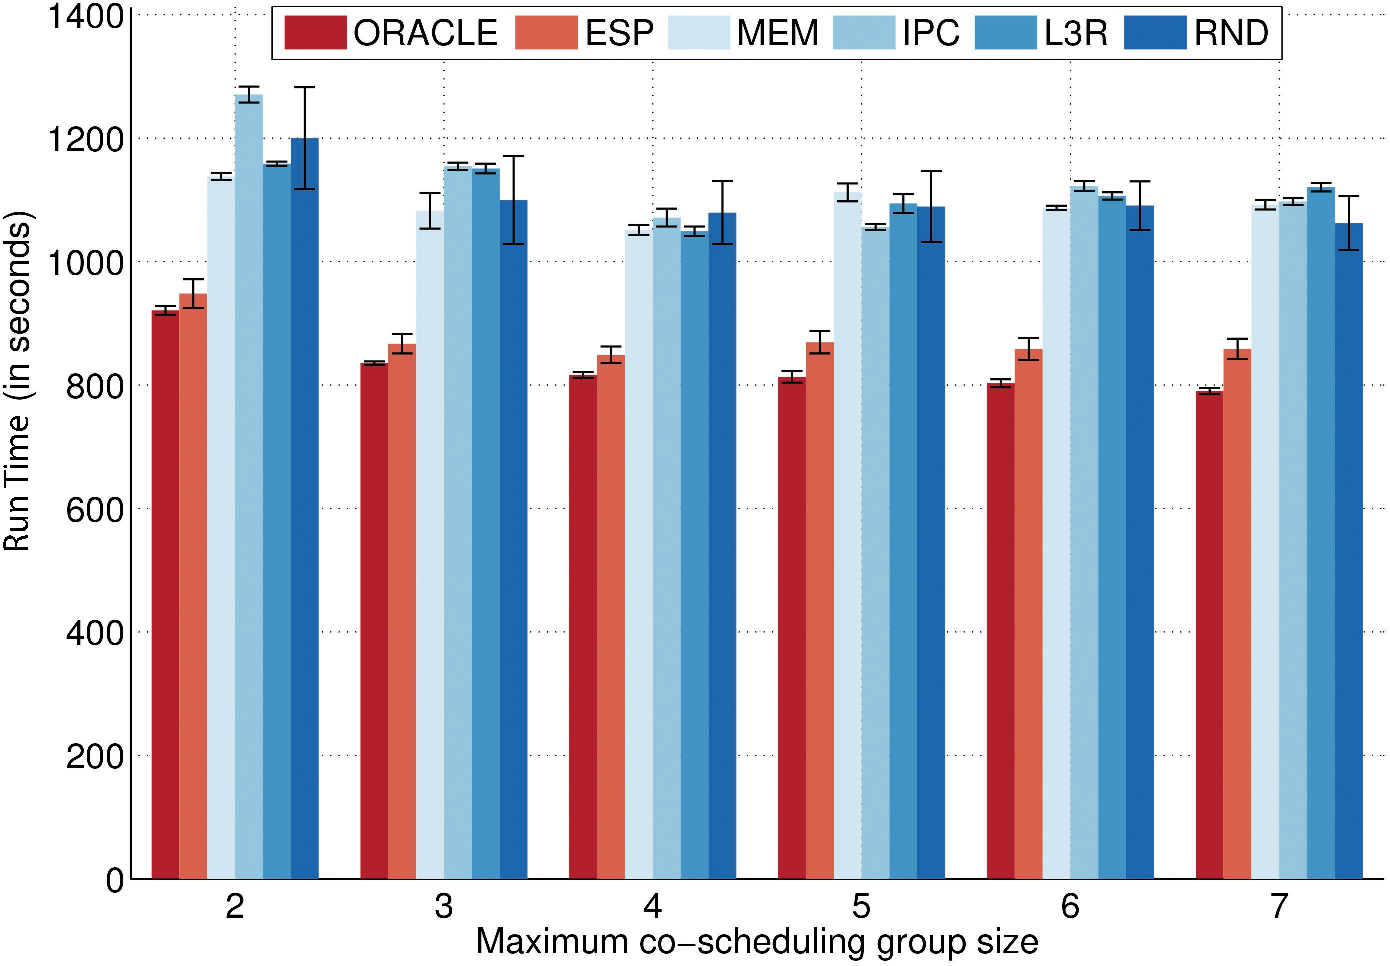
\includegraphics[width=0.7\textwidth]{figures/barmainCOPY.pdf}
 \caption{\small Single processor scheduling performance. On an
   average over different $k$, \SYSTEM{} is 25\% better than MEM, 29\%
   better than IPC, 27\% better than L3R, 26\% better than RND, and
   only 5\% worse than ORACLE. }
\label{fig:bar_single_processor}
\end{center}
\end{figure}

\begin{figure*}[t]
  \begin{center}
    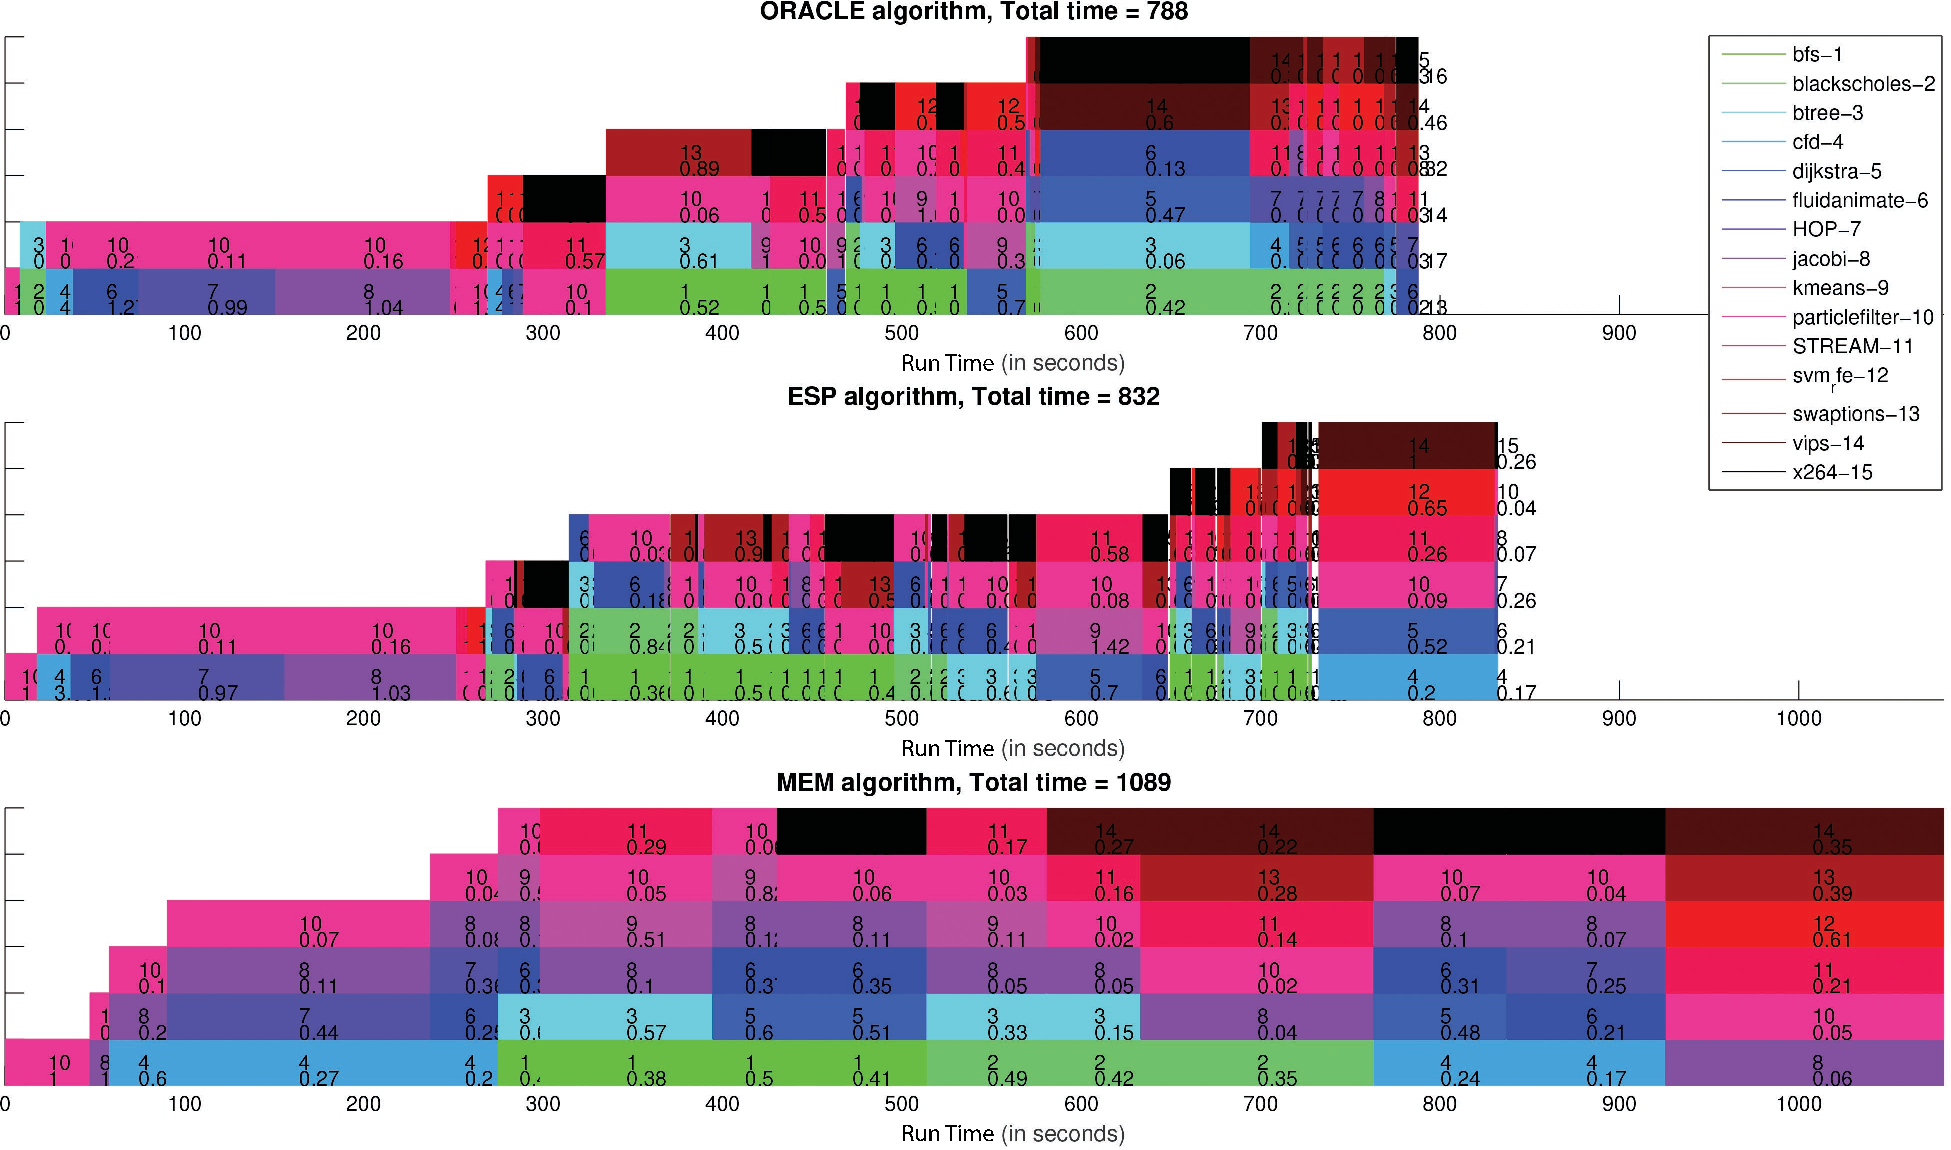
\includegraphics[width=1\textwidth]{figures/scheduleCOPY.pdf}
    \caption{\small Comparison of schedules obtained from different
      algorithms with up-to 6 co-scheduled applications ($k$ = 6) (more
      compact is better). Each block represents an application running
      with other applications. The number in the top of the block
      represents the application index. The number at the bottom
      represents the slowdown the application experiences.  The
      schedule built using \SYSTEM{} algorithm squeezes the
      applications together better than the MEM baseline.}
    \label{fig:schedule2}
  \end{center}
\end{figure*}
\begin{figure*}[t]
\begin{center}
 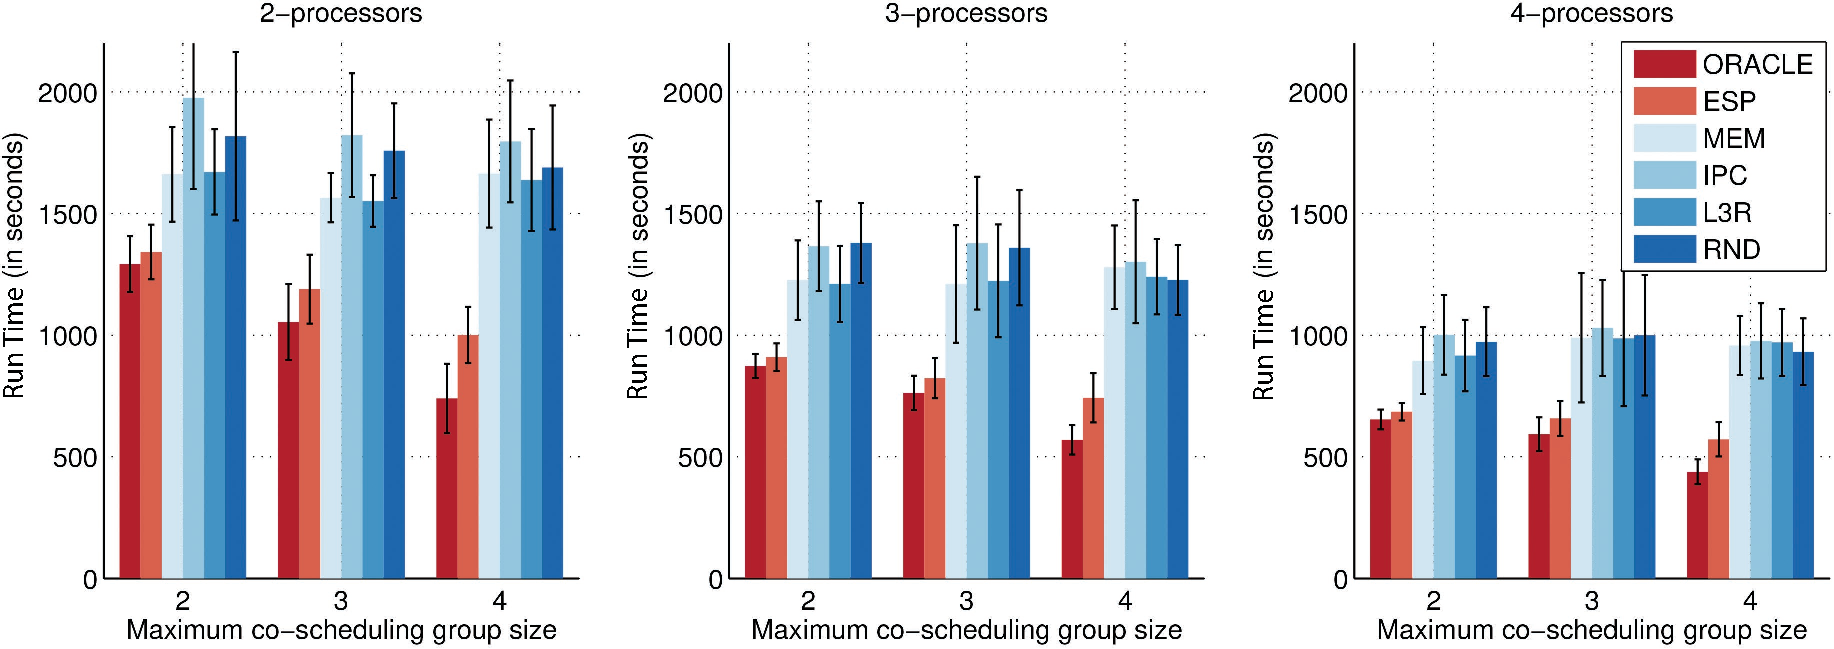
\includegraphics[width=1\textwidth]{figures/parallel_schedule_combb_all_mayCOPY.pdf}
 \caption{\small Comparison of multi-node scheduling times for stream
   of 40 applications (lower is better). On an average over different
   processes and tuples, \SYSTEM{} is 47\% better than MEM, 61\%
   better than IPC, 47\% better than L3R and 54\% better than RND. }
\label{fig:expt:multi-node-all}
\end{center}
\end{figure*}

\begin{figure*}[!t]
\begin{center}
 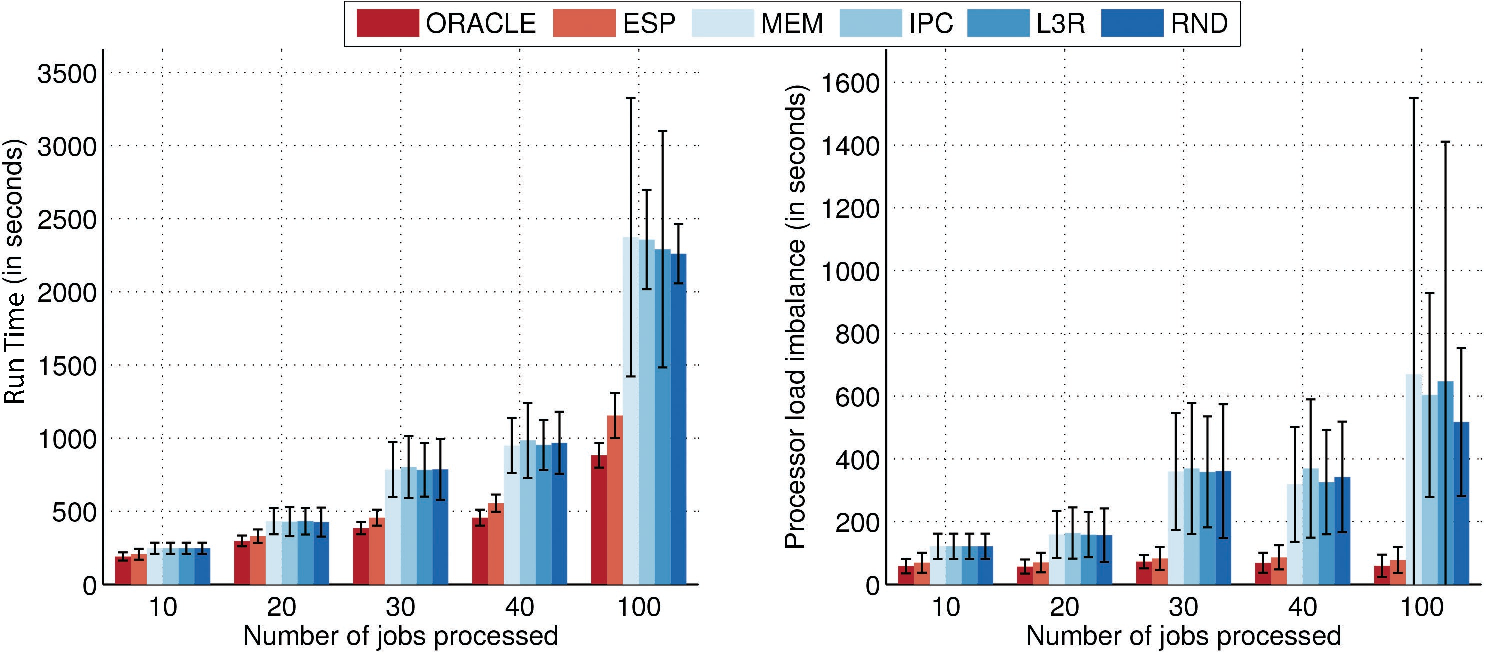
\includegraphics[width=0.9\textwidth]{figures/parallel_schedule_combb_100jobs_load_4_4_load_imbalance_combinedCOPY.pdf}
 \caption{\small Multi-node scheduling performance with varying number
   of incoming jobs, allowing up to 4 co-scheduled applications per
   node (lower is better). The left figure shows scheduling time (in
   seconds) -- on average \SYSTEM{} is 60\% better than MEM, 61\%
   better than IPC, 58\% better than L3R and 58\% better than RND. The
   right figure shows the load imbalance (the difference between the
   highest and lowest scheduling time across nodes).  As we increase
   the number of jobs the load imbalance increases faster for the
   baseline algorithms and seems relatively constant for \SYSTEM{} and
   the ORACLE.}
\label{fig:expt:multi-node-100}
\end{center}
\end{figure*}

\subsection{Single Node Scheduling Results}
\label{sec:sched_single_proc}
To test single-node batch scheduling, we launch all 15 benchmarks
listed in \secref{setup}.  The schedulers order application execution
to minimize total job completion time.  We vary $k$, the maximum
number of applications that can be co-scheduled from two to six.  We
find that it is never beneficial to schedule more than six
applications simultaneously and no scheduler (other than random) ever
attempted to do so even when more were allowed.  We run 15 separate
experiments for each $k$, where each experiment differs by the split
between training and testing data for \SYSTEM{}.


\figref{fig:bar_single_processor} shows the results. The x-axis is
$k$, the y-axis is the time to complete the work, and there is a bar
showing the mean scheduling time for each of our points of comparison
with an error bar showing one standard deviation.
During the offline phase, we first sample a few configurations
followed by calculating the estimated performance those samples;
overhead of which is discussed in the next section(Section
\secref{expt:overhead}). Once we do the estimation of the performance
using \SYSTEM{} individually for each $k = 2:6$ ($k$ denotes the
maximum number of applications we are willing to co-schedule
together), we run Algorithm \ref{alg:ItrSched-multi} to schedule those
applications. We notice that, as per our intuition, as we allow more
applications to run together, the scheduling time for the ORACLE
decreases. But, the scheduling time does not decrease significantly
after 4-tuples. On the other hand for \SYSTEM{} the scheduling time
decrease until 4-tuples and slightly increases after that. We
attribute this to the fact that as we estimate more tuples the overall
estimation error is piling up and since the benefit of running more
applications together dwindles after 4-tuples, the extra noise in the
system makes approximate scheduling using \SYSTEM{} slightly worse. We
see similar behavior for scheduling even in the baseline algorithms,
where we see improvement only up-to a certain point.
Overall, \SYSTEM{} performs much better than the baseline algorithms
and only slightly worse than the ORACLE. On average over different
$k$, \SYSTEM{} is 25\% faster than MEM, 29\% faster than IPC, 27\%
faster than L3R and 26\% faster than RND.  These results include
prediction and scheduling overhead, yet \SYSTEM{} is only 5\% worse
than the ORACLE, which has no overhead and knows the future.  We
conclude that \SYSTEM{} produces highly accurate predictions and yet
is efficient enough for practical use.


To provide intuition on the different schedulers,
\figref{fig:schedule2} illustrates the schedules produced by: ORACLE
(top), \SYSTEM{} (middle), and MEM (bottom) when they are allowed to
co-schedule up to six applications.  For each chart, the horizontal
axis represents time in seconds. Each colored block represents an
application running with other applications. The top number in the
block represents the application index (see the legend for mapping
from index to name), and the bottom number represents the actual
slowdown the application experienced at that time (this actual
slowdown is determined after the fact).  A better schedule is more
compact and completes further to the left.  Clearly, \SYSTEM{}'s
schedule is more compact and closer to the ORACLE than MEM.  ORACLE
runs the maximum number of applications together less than half of the
time.  MEM, in contrast, runs the maximum allowed number of
applications most of the time. Overall in this particular instance,
the scheduling time for the ORACLE is 788 seconds, 832 for \SYSTEM{},
and 1089 for MEM.




\subsection{Multi-node Scheduling Results}
\label{sec:sched-multi-node}
In this section we discuss multi-node scheduling performance. We use
two, three, and four copies of our base test platform (described
above).  We assume that applications arrive randomly from our set of
15 benchmarks (so some benchmarks may have multiple instances live in
the system).  The challenge is to assign an application to a
processor as it arrives such that the total impact on the system is
minimized; \ie put the application on the node that minimizes
interference.

The oracle computes the best possible schedule, the heuristics use
activity vectors to select the best node and the \SYSTEM{}-based
approach uses Algorithm \ref{alg:ItrSched-multi}.
\figref{fig:expt:multi-node-all} summarizes the results for 2, 3 and 4
processors and for $k = 2,3$ or $4$. As we increase the number of
processors, the scheduling time improves for all approaches. \SYSTEM{}
performs almost as well as the ORACLE, performing 5\% to 13\% worse on
an average.  In fact, \SYSTEM{} is always within 1 standard deviation
of ORACLE. \SYSTEM{} performs significantly better than the activity
vector algorithms. On average over different processes and tuples,
\SYSTEM{} is 47\% better than MEM, 61\% better than IPC, 47\% better
than L3R, and 54\% better than RND.  Additionally, the standard
deviation in performance for \SYSTEM{} is much lower compared to the
baseline algorithm, leading to much better performance predictability.
This predictability is further evidence of our claim that \SYSTEM{}
allows the schedulers to avoid bad predictions.

\subsection{Multi-node Sensitivity to Job Size}
\label{sec:exp:multi-node-job}
We also study the scheduling performance as a function of the total
number of applications scheduled. To be clear, jobs are still
scheduled as they arrive (the multi-node scheduler does not reorder
applications), we simply have more of them.  Specifically, we send up
to 100 jobs to a system with 4 nodes and we are allowed to co-schedule
up to 4 applications together.  For each experiment, we perform 15
trials with different random job arrivals.  All results report the
mean with error bars indicating one standard deviation.

\figref{fig:expt:multi-node-100} shows how scheduling performance
changes as a function of the total number of applications scheduled.
The figure consists of two charts: the one on the left showing
scheduling time as a function of applications scheduled and the one on
the right showing load imbalance in terms of the largest difference in
execution time between one processor and another. The number of
applications scheduled is shown on the x-axis and the time on the
y-axis.  As the number of applications increases, \SYSTEM{}'s relative
performance improves compared to the activity vector approaches. The
key to this result is \SYSTEM{}'s accurate quantification of
interference.  The ability to directly reason about slowdown allows
the \SYSTEM{}-based approach to rank scheduling decisions and always
choose the one with the least impact on the performance of both the
running applications and the application that just arrived.

\SYSTEM{}'s foresight becomes more crucial as the number of jobs
increase because bad decisions can create severe load imbalance on the
parallel machine, as shown on the right side of
\figref{fig:expt:multi-node-100}. As we increase the number of jobs
the processor load imbalance increases vastly for the activity vector
approaches and seems relatively constant for \SYSTEM{} as well as
ORACLE. On an average \SYSTEM{} is 60\% better than MEM, 61\% better
than IPC, 58\% better than L3R and 58\% better than RND. Again, the
standard deviation (shown by the error bars) for \SYSTEM{} is much
lower than the baselines---leading to much more predictable
performance for latency sensitive applications.


\begin{figure*}[t]
\begin{center}
 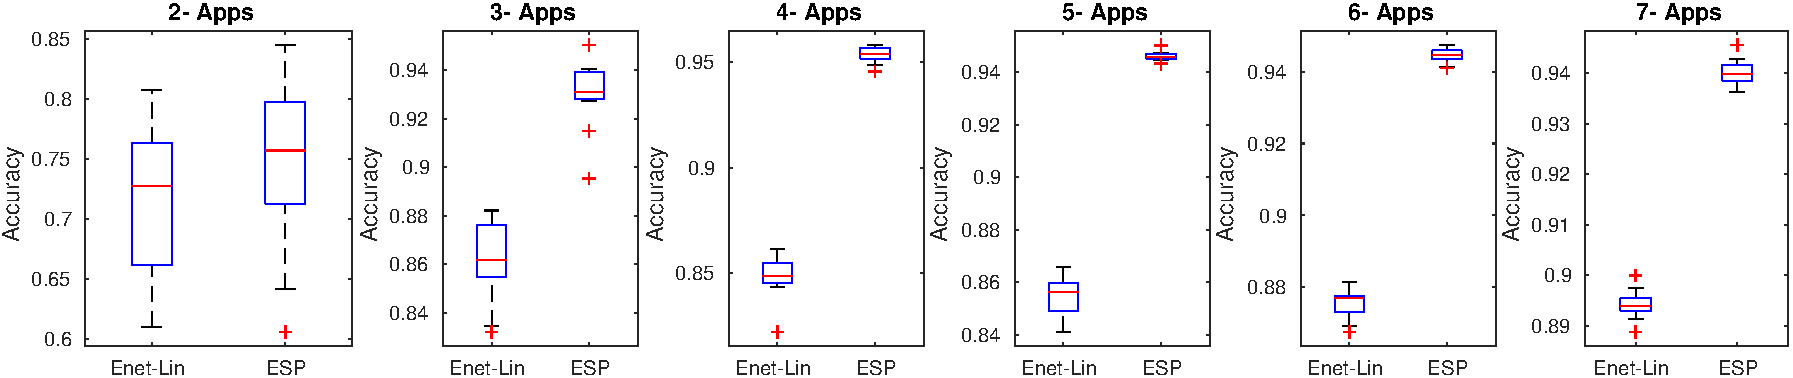
\includegraphics[width=1\textwidth]{figures/accuracy_boxplot_ridge_lasso_enet2.pdf}
 \caption{\small Prediction accuracy comparison between Enet-lin and
     \SYSTEM{}.
     % We use 70\% of the data during training phase and
     %  predict the remaining 30\% of the samples.
   }
\label{fig:est:box-plot}
\end{center}
\end{figure*}
\PUNT{
\begin{table*}[t]
\centering
\caption{Overhead}
\footnotesize
\begin{tabular}{ c|c|c|c|c|c|c|c }
 \hline
 \hline
 &k & 2 & 3 &4 & 5 & 6 & 7 \\
 \hline
\multirow {3}{*}{\SYSTEM{}}  & Model training (in seconds)   & 0.42    & 0.59 &   0.68 & 0.69 & 0.48 & 0.51\\
& Prediction time (in seconds)  &   0.00056  & 0.003   &0.0076 & 0.0198 & 0.04 & 0.06\\
& Training sample size (in \%)  & 70\% & 40 \% &  10 \% & 4\% & 1 \% & 1\% \\ \hline \hline
\multirow {2}{*}{Scheduling Algorithm \ref{alg:ItrSched}}  & \SYSTEM{} (in seconds)    &0.52 & 1.18&  2.08 & 3.17 & 4.19 & 5.57\\
& Linear program (in seconds) &   0.12 & 0.21 & 0.35 & 0.9 & 1.75 & 3.3 \\
 \hline
 \hline
\end{tabular}
 \label{table:overhead}
\end{table*}
}

\begin{table*}[t]
\centering
\caption{Overhead}
\footnotesize
\begin{tabular}{ c|c|c|c|c|c|c|c }
 \hline
 \hline
 &k & 2 & 3 &4 & 5 & 6 & 7 \\
 \hline
\multirow {3}{*}{\SYSTEM{}}  & Model training (in seconds)   & 0.42    & 0.59 &   0.68 & 0.69 & 0.48 & 0.51\\
& Prediction time (in seconds)  &   0.00056  & 0.003   &0.0076 & 0.0198 & 0.04 & 0.06\\
& Training sample size (in \%)  & 70\% & 40 \% &  10 \% & 4\% & 1 \% & 1\% \\ \hline \hline
\multirow {1}{*}{Scheduling Algorithm \ref{alg:ItrSched}}  & Linear program (in seconds/job) &   0.008 & 0.014 & 0.023 & 0.06 & 0.117 & 0.22\\
 \hline
 \hline
\end{tabular}
 \label{table:overhead}
\end{table*}

\subsection{\SYSTEM{} Prediction Accuracy}
\label{sec:st_model}
%The preceding sections show the benefits of integrating \SYSTEM{} into
%single and multi-node schedulers.  We assert that \SYSTEM{}'s accurate
%quantifiable predictions are the key to its success.  Here we analyze
%that accuracy directly.


\subsection{\SYSTEM{} Accuracy versus the Collaborative filter Algorithm}
\begin{figure}[!t]
  \begin{centering}
 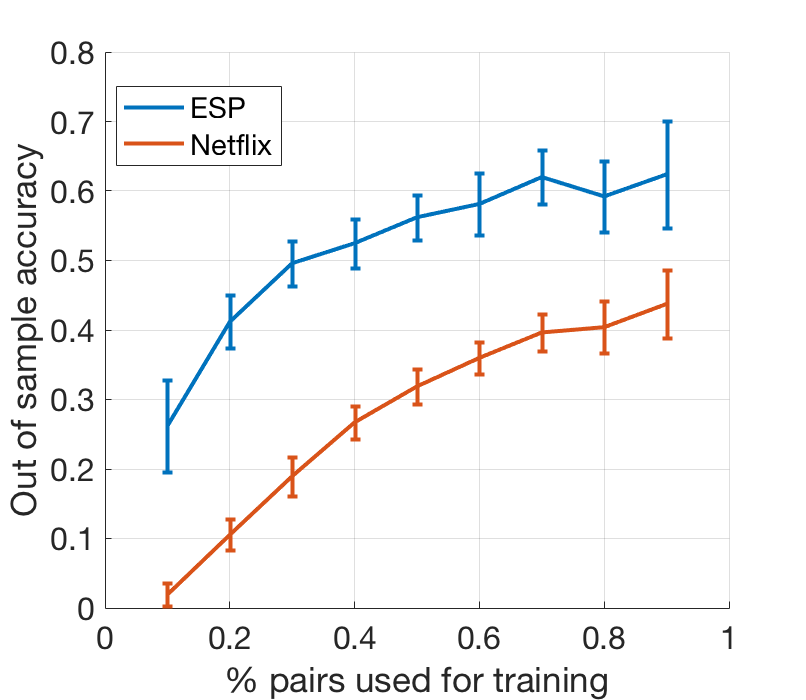
\includegraphics[width=0.5\columnwidth]{figures/accuracy_netflix_vs_esp.png}
 \caption{Sample complexity plot for Collaborative filter algorithm used by Paragon}
 \end{centering}
\label{fig:netlix}
\end{figure}
We compare \SYSTEM{}'s accuracy to that of collaborative filtering;
\eg{} the Collaborative filter algorithm, which is used by other machine-learning
based interference predictors \cite{paragon,quasar}.  Specifically, we
use collaborative filtering to predict which pairs of applications
will work well together.  The intuition is that if two applications we
have never run together work well with some third application, they
may work well together themselves.

\PUNT{\figref{fig:accuracy_netflix} Figure \figref{fig:netflix}} Figure 5.6 compares the accuracy of the
Collaborative filter algorithm and \SYSTEM{} for predicting the interference of
pairs of applications.  The y-axis shows accuracy and the x-axis shows
the percentage of samples.  This experiment shows that \SYSTEM{}
always outperforms collaborative filtering for our benchmarks.  These
results demonstrate the importance of incorporating low-level features
into the prediction.
We compare \SYSTEM{} with the \textit{elastic-net} regularization
method on the linear model (\textit{Enet-lin}) described in
\secref{est:elastic-net}.  \PUNT{The comparisons are based on
  prediction accuracy for both the models.  vs sample complexity,
  specifically how many samples are required to reach 90\% accuracy.
  Throughout this section, we refer to one sample as a measurement of
  a group of $k$-applications which generates $k$ readings
  corresponding to each of the applications in the group.} To evaluate
quantitatively, we measure the \emph{accuracy} of the predicted
performance $\hat{\z}$ with respect to the true data $\z$, by
computing the \emph{coefficient of determination} ($R^2$ value):
\begin{equation}
\label{eq:accuracy}
\text{accuracy}(\hat{\z},\z) = \left(1 - \frac{\| \hat{\w}-\w \|^2_2}{\| \w - \bar{\w}\|^2_2}\right)_{+},
\end{equation}
where $\w = \min(\z,\boldsymbol{1})$ and $\hat{\w} =
\min(\hat{\z},\boldsymbol{1}).$ This metric captures how well the
predicted results correlate with the measured results. Unity
represents perfect correlation.



%\subsubsection{Prediction accuracy}
\figref{fig:est:box-plot} shows a box-plot for out-of-sample
predictive accuracy of \SYSTEM{} and Enet-lin when we train both the
models with 70\% data and test the prediction on the remaining data.
For $k=2$, \SYSTEM{} performs only slightly better than the Enet-lin
with on average 76\% accuracy whereas the baseline is 73\% accurate.
For $k>2$, the prediction accuracy for the \SYSTEM{} varies from 93\%
to 96\% with very small variance. On the other hand, Enet-lin is only
between 85\% to 88\% accurate.

\begin{figure*}[!htbp]
\begin{center}
 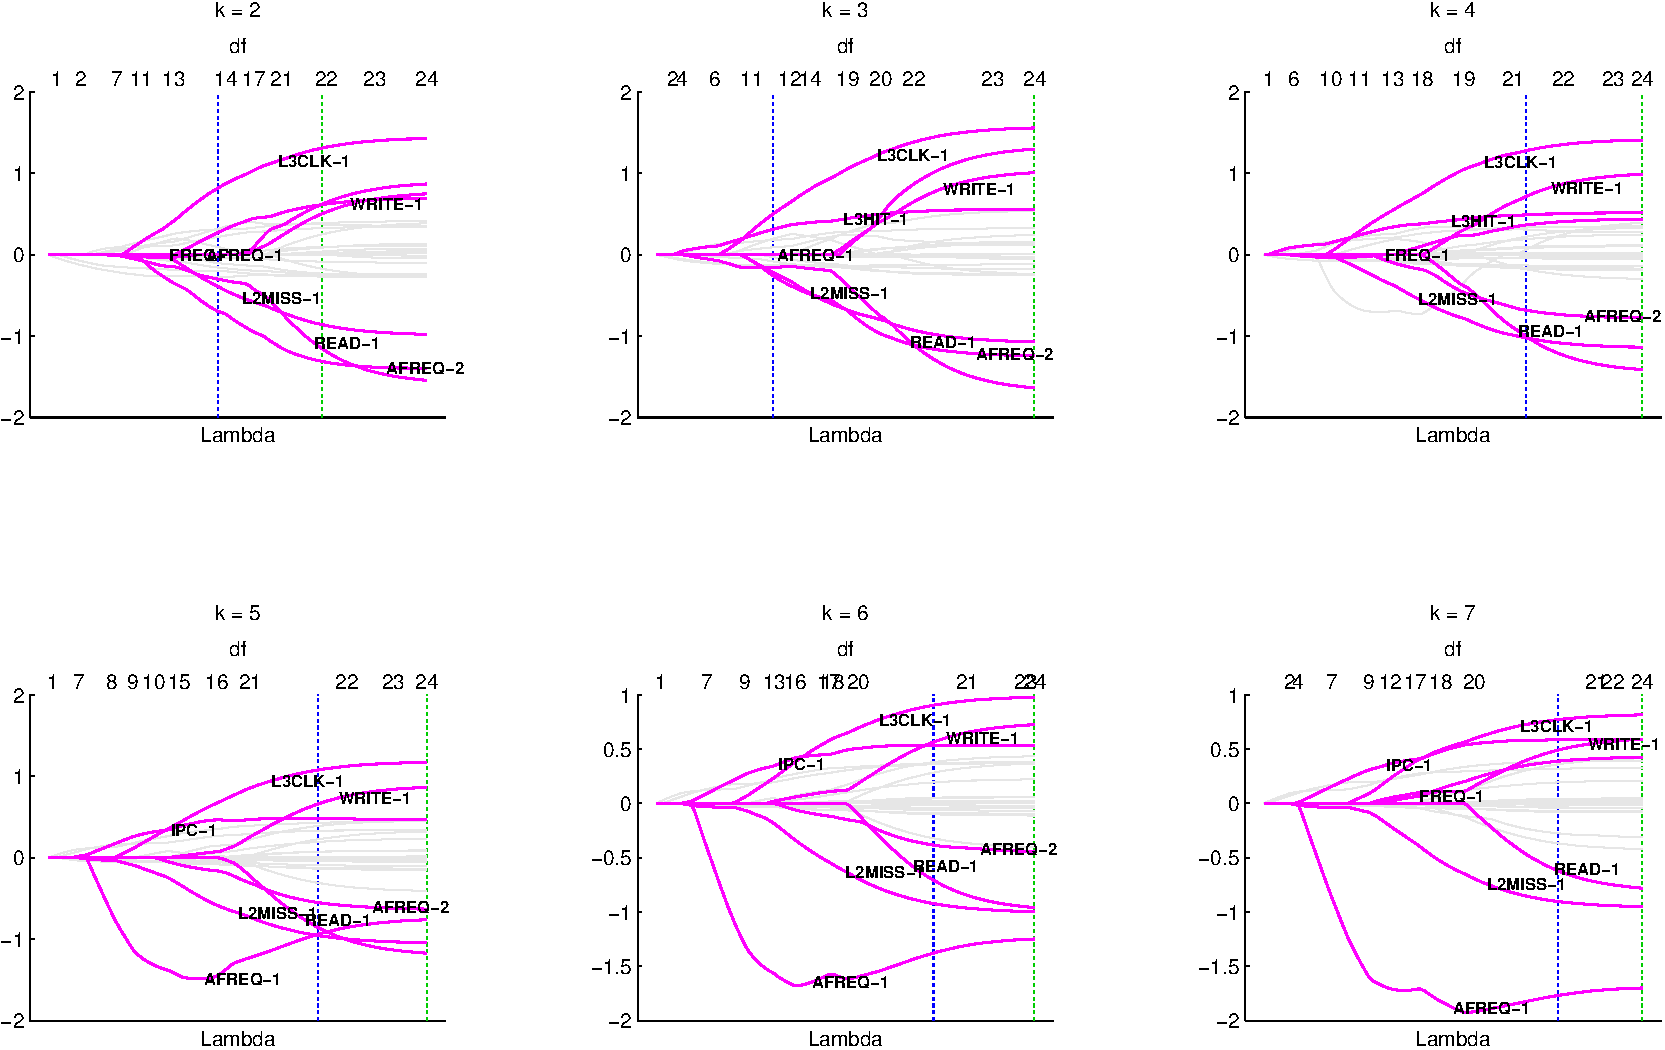
\includegraphics[width=1\textwidth]{figures/solution_path_general.pdf}
 \caption{ A solution path diagram using elastic-net for a linear model (no interaction terms) with just an important subset of variables so that it is easier to visualize.  Each dark solid line in the plot represents a variable's coefficient. The corresponding variable is mentioned on the line. The dashed blue line indicates largest $\lambda$ such that MSE is within one standard error of the minimum, a scalar and the dashed green line corresponds $\lambda$ value with minimum MSE.  Since, the variables in the design matrix are highly correlated, variable signs may not be correctly represented.}
\label{fig:est:solution-path}
\end{center}
\end{figure*}
\subsubsection{Discussion for the solution path for regression models}
We wanted to build some more intuition about the variable selection
and how the model evolves over different values for $k$. In
\figref{fig:est:solution-path}, we show a variable in and out plot and
what is known as a \textit{solution path} in statistics. The x-axis is
the regularization parameter $\lambda$ and y-axis is the coefficient
size. For the co-efficient size to relatively make sense we have
normalized the columns of the design matrix to have Euclidean-norm
equal to 1. As we increase $\lambda$ the regularization becomes less
strict and more and more variables can enter the model. In this figure
we have a solution path diagram using elastic-net for a linear model
(no interaction terms) with just an important subset of variables so
that it is easier to visualize.  Each dark solid line in the plot
represents a variable's coefficient and how it changes as we increase
lambda.  The corresponding variable is mentioned on the solid plot
line itself. The dashed blue line indicates largest $\lambda$ such
that MSE is within one standard error of the minimum, a scalar and the
dashed green line corresponds $\lambda$ value with minimum MSE.
Since, the variables in the design matrix are highly correlated, a
positive (or a negative) variable in this diagram does not mean that
it certainly positively (or negatively) affects the performance. But,
if the variable has large absolute value, we can still claim that,
conditioned on other variables selected in the model it has large
impact. What is interesting in this figure is how as $k$ increases the
model evolves. $k=2, 3$ and $4$ have similar solution paths and $k=5,
6$ and $7$ has similar path but the two paths are a bit different from
each other, indicating some phase transition happening at $k=4$. This
indicates that there might be an opportunity to predict performance
for larger $k$'s by aggregating data for smaller $k$. This can be very
important for datacenters where they only observe very large number of
applications co-scheduled together.



\subsection{Overhead}
\label{sec:expt:overhead}
\SYSTEM{} has an offline sampling phase followed by an
estimation phase. Once we have collected the samples from the batch of
co-scheduled applications, we run \SYSTEM{} to obtain the predictions
for the rest of the combinations of the applications. We have
summarized the overhead results in the Table \ref{table:overhead}. We
require less than 0.7 seconds to build the performance model for a
batch of $k$-tuples running together. Once the model is built, the
prediction time for \SYSTEM{} is very small and would range from 0.5
milliseconds to 60 milliseconds. For such small training data, the
prediction accuracy for $k=2$ is around $80\%$ and for $k>2$ it is
around $86\%$.

The scheduling overhead, again has two components: first obtaining the
application's batch run profile which is done using \SYSTEM{}, and
then solving the linear program to obtain the schedule. The first part
(in the top of Table \ref{table:overhead}) is done offline.  The vast
bulk of online work is done by Equation \eqref{eq:schedule_general2},
which solves a very sparse optimization problem. The total overhead
per scheduled job for Algorithm \ref{alg:ItrSched} -- the online
portion of the approach -- ranges from 0.008 seconds for $k=2$ to 0.22
seconds for $k=7$. Almost all of this work could be parallelized on a
multicore (or accelerated with SIMD instructions) but that is beyond
the scope of this work.  We note that it is quite practical to
consider co-scheduling up to 4 jobs.  The overhead of scheduling $7$
jobs may become prohibitive, but it is never useful on our test
system.  This is not an insignificant amount of time but this approach
is suitable for long running applications and the benchmarks that we
have used in this work are all long running benchmarks with at least
10 seconds of individual runtime.

\section{Related work}
Accurate performance estimates are essential for solving scheduling
and resource allocation problems \cite{chiang2002impact}.  Accurate
estimates are difficult to obtain due to the complexity and diversity
of large-scale systems \cite{kanev2015profiling}.  A particular
challenge is modeling performance loss due to contention among
applications \cite{kambadur2012measuring}.  Better contention models
could improve system utilization while ensuring quality-of-service in
latency sensitive applications \cite{Bubble-flux}.

Several approaches investigate statistical and machine learning
techniques for estimating power, performance, and energy of a single
application running on a single system.  Many of these approaches
improve the time of developing new hardware designs, but are not
suitable for online resource management
\cite{Yi2003,LeeBrooks2006,CPR}.  Other approaches can predict the
power and performance of various resource allocations to single
applications \cite{Koala} or optimize energy efficiency under latency
constraints \cite{LEO}.  A recent approach combines machine learning
with control theory to guarantee energy consumption, but only for a
single application \cite{JouleGuard}.  Perhaps most similar to
\SYSTEM{} is the Mantis project which also uses higher-order
regularized regression models (based on Lasso) to predict smartphone
app performance \cite{kwon2013mantis}.  Mantis, however, does not
predict contention among multiple applications, which is \SYSTEM{}'s
focus.

Other approaches predict and mitigate contention in single-node
systems.  Many decide to co-schedule or not, but they do not produce
quantitative slowdown estimates.  For example, Dwyer et al. propose a
classifier that predicts whether contention will be high or low, but
this approach does not produce a numerical estimate
\cite{dwyer2012practical}.  Similarly, ReSense detects highly
contended resources and reacts to reduce that contention, but it never
estimates contention \cite{resense}. Another approach estimates
throughput (total system performance), but does not produce estimates
of individual application performance
\cite{xu2010cache,chen2010performance}.  Subramanian et al. propose an
approach that does produce accurate estimates of performance (within
9.9\%) based on only last-level cache access rate and memory bandwidth
\cite{subramanian2015slowdown}.  These results are achieved on a
simulator rather than a real system, however, and on our real system
these two features are not sufficient to predict contention with any
level of accuracy.  Another single-node system, D-Factor, uses
non-linear models to predict the slowdown of a new application given
current resource usage \cite{Lim2012dfactor}.  Unlike \SYSTEM{},
D-Factor is not capable of predicting how two applications will
interfere with each other if neither is currently running.

Several approaches estimate and mitigate contention to schedule for
multi-node systems.  The activity vectors approach works on single or
multi-node systems by maximizing the variance among resource usage in
co-scheduled applications \cite{merkel2010resource}.  This heuristic
makes intuitive sense -- applications with very different resource
needs are less likely to interfere with each other -- but this
approach does not produce quantitative estimates and therefore can
make bad decisions when contention is unavoidable.  Merlin, is
somewhat similar, in that it tries to estimate contended resources and
migrate virtual machines to areas of lower contention, but it also
does not produce slowdown estimates \cite{Merlin}.  DejaVu is a
machine learning approach that classifies application workloads and
then schedules according to known good schedules for the
classification \cite{dejavu}. DejaVu creates an \emph{interference
  index} which can be used to rank slowdowns and migrate VMs or
reallocate resources, but it does not produce accurate estimates of
the actual slowdowns incurred.  Similarly, Quasar \cite{quasar} and
Stay-Away \cite{stay-away} use classification schemes to predict and
mitigate interference, but neither produces performance estimates in
the face of interference.  Bubble-flux \cite{Bubble-flux}, an
improvement over the earlier Bubble-up \cite{Bubble-up} does produce
slowdown estimates and, like \SYSTEM{}, it is efficient enough to
consider interference among more than two applications.  The main
difference between Bubble-flux and \SYSTEM{} is that Bubble-flux uses
no offline prior information and must dynamically probe the system.
This lack of prior information means that Bubble-flux must suffer
either poor utilization or inaccurate schedules during the probing
phase.  \SYSTEM{} uses a highly accurate offline model and combines
that with online updates to its predictions to further improve
accuracy while making use of the vast amount of data available to
inform offline model building.

%\TODO{One paragraph on stats related work.}
We model interference estimation as a \emph{high-dimensional}
regression problem with prohibitively many dimensions.  Many
statistical methods address high-dimensionality (\eg SURE
\cite{fan2008sure}). In computer system performance, however,
measurable features are highly correlated and existing methods do not
provide high accuracy.  Other statistical models emit more accurate
predictors given correlated features (\eg \cite{yuan2006model} and
\cite{bien2013lasso}), but they do not scale to our problem size.
Even though we make a strong assumption that the interaction terms are
present only if their individual linear terms are significant, the
heuristic has very high accuracy and produces good schedules in
practice.

\section{Conclusion}
This paper explores machine learning methods for predicting
application interference in computing systems.  Specifically, we
explore several state-of-the-art regularization techniques for
high-dimensional problems---when many more features are available than
samples---and we conclude that existing linear techniques are not
accurate enough, while existing higher-order techniques are accurate
but slow.  Inspired by these observations we present \SYSTEMESP{}, a
combination of linear feature selection with higher-order model
building that achieves the practicality of linear models with the
accuracy of higher-order models.  We have demonstrated that
\SYSTEMESP{}'s quantitative predictions produce significantly better
schedules than existing heuristics for both single and multi-node
systems, with up to 1.8$\times$ improvement in application completion
time and significantly lower variance.  Additionally, \SYSTEMESP{}
achieves much higher prediction accuracies than prior
approaches---over 93\% when considering three or more applications.
We have made the source code available so that others may improve on
or compare with \SYSTEMESP{}.


\chapter{Performance and power estimation}
\section{Introduction}
% Dennard Scaling making energy essential.  Architects address energy
% by making more complicated processors which expose resources to
% software management.  For a wide range of applications, need to meet
% performance goals with minimal energy.
Large classes of computing systems---from embedded to cloud---must
deliver reliable performance to users while minimizing energy to
increase battery life or decrease operating costs.  To address these
conflicting requirements, hardware architects expose diverse,
heterogeneous resources with a wide array of performance and energy
tradeoffs.  Software must allocate these resources to
guarantee performance requirements are met with minimal energy.


% Difficulties of meeting performance with minimal energy. (1)
% complexity---heterogeneous resources---and (2) dynamics---adjust to
% unforeseen changes in workload and environment.
There are two primary difficulties in determining how to allocate
heterogeneous resources.  The first is \emph{complexity}: resources
interact in complicated ways, leading to non-convex optimization
spaces.  The second is \emph{dynamics}: perfor\-mance requirements
must be met despite unpredictable disturbances; \eg{} phases in input
or changes in operating environment.  Prior work addresses each of
these difficulties individually.

% Prior approaches addressed each of these difficulties individually.
% ML---can handle complexity.  ML advantages: can handle
% non-convexity, avoid local optima, get to true optimal solution. ML
% disadvantages: advanced techniques are expensive and no notion of
% dynamics.  Control---handles dynamics.  Control advantages: formally
% analyzable guarantees despite dynamics.  Control disadvantages:
% relies on good models---no local optima, bounded error.
Many machine learning approaches model the complex performance/power
tradeoff spaces inherent to heterogeneous computing
\cite{reddiHPCA2013,dubach2010,Bitirgen2008,Ipek,Koala,LEO,Flicker,Ponamarev,Paragon}.
Learning handles non-convexity, identifying local optima and moving to
globally optimal solutions. These techniques are computationally
expensive and lack support for dynamics; \ie{} when the environment
changes the expensive model building process must be restarted.
Control theoretic solutions provide formal guarantees that they will
converge to the desired performance despite system dynamics
\cite{Hellerstein2004a,Chen2011,POET,ControlWare,Agilos,grace2,JouleGuard}.
Control provides formal guarantees of convergence to the desired
performance, but these guarantees require \emph{ground truth} models
and control will not converge if the models do not accurately capture
system complexity---including local optima and non-linearities.


% Want to combine learning and control to address both difficulties
% simultaneously.  Need an interface that allows learned models to be
% used by control system.  Challenges: (1) overhead and (2) formal
% guarantees.  
We want the benefits of both learning and control to ensure
performance requirements are met with minimal energy in complex and
dynamic environments.  Thus, we present
\SYSTEM{}:\footnote{\textbf{C}ontrol \textbf{A}nd \textbf{L}earning
  for \textbf{O}ptimal \textbf{R}esource \textbf{E}nergy
  \textbf{E}fficiency} a \emph{parameter-free} framework for combining
machine learning and control theory to build resource allocators.
\SYSTEM{} is parameter-free because it automatically tunes all
internal parameters and models to customize itself to the application
under management.  In contrast, many approaches require user-specified
parameters, like learning rate \cite{dubach2010,Tokic2010} or poles
and zeros of characteristic equations \cite{ControlWare,POET}.

\SYSTEM{} creates a general control system implementation that factors
out the parameters that must be learned.  While traditional control
designs assume all combinations of resource configurations have been
measured accurately (requiring 100s or 1000s of samples
\cite{sysid,FSE2015}), \SYSTEM{} tunes its internal models and
parameters while sampling only a small subset of possible
configurations.  Among these, the controller's \emph{pole} is a key
parameter.  \SYSTEM{} automatically tunes the pole, providing formal
guarantees the controller converges to the desired performance---even
when behavior is estimated by a noisy learner rather than directly
measured.  \SYSTEM{} implements modular abstractions and self-tuning
mechanisms such that the expensive learning can be offloaded to
another system and the controller itself runs in
constant---$O(1)$---time.  Thus, learning's high cost can be amortized
as \SYSTEM{} uses \emph{transfer learning} to apply knowledge from
multiple devices and applications \cite{pan2010survey}.


\SYSTEM{}'s generality allows a wide range of learning techniques to
be paired with its controller.  So, \SYSTEM{} not only provides an
advantage over existing individual learning and control techniques, it
allows us to explore different combinations of learning and control to
find the best.

% Implement CALOREE.  Test against state of the art learning and
% self-tuning control systems.  We find that:
We evaluate \SYSTEM{} by implementing the learner on an x86 server and
the controller on heterogeneous ARM big.LITTLE devices.  We compare
\SYSTEM{} to existing, state-of-the-art learning (including polynomial
regression \cite{Koala,dubach2010}, the Netflix algorithm
\cite{netflix,Paragon}, and a hierarchical Bayesian model \cite{LEO})
and control (including proportional-integral-derivative
\cite{Hellerstein2004a} and adaptive, or self-tuning
\cite{HandbookControl}) techniques.  \PUNT{Additionally, we compare to
  a naive combination of learning and control that does not account
  for the inaccuracies of learned models.}  We set performance
goals---as latency requirements---for a set of benchmark applications
and then measure both the percentage of time the requirements are
violated and the energy for each application.  We test both
\emph{single-app}, where an application runs alone, and
\emph{multi-app} environments, where other applications enter the
system and compete for resources.  \SYSTEM{} achieves the:
\begin{itemize}[leftmargin=1em]
\item \textit{Most reliable performance:}
  \begin{itemize}[leftmargin=1em]
  \item In the \emph{single-app} case, the best prior technique misses
    12\% of deadlines on average, while \SYSTEM{} misses only 5\% on
    average---reducing deadline misses by more than 58\% compared to
    prior approaches.
  \item In the \emph{multi-app} case, the best prior approach averages
    30\% deadline misses, but \SYSTEM{} misses just 5.6\% of
    deadlines---a huge improvement over prior work.
  \end{itemize}
\item \textit{Best energy savings:} We compare to an \emph{oracle}
  with a perfect model of the application, system, and future events.
  \begin{itemize}[leftmargin=1em]
  \item In the \emph{single-app} case, the best prior approach
    averages 12\% more energy consumption than the oracle, but
    \SYSTEM{} consumes only 5\% more.
  \item In the \emph{multi-app} case, the best prior approach averages
    18\% more energy than the oracle, while \SYSTEM{} consumes just
    8\% more.
  \end{itemize}
\end{itemize}

% Key contributions.
% Contributions, but I decided against bulleted llist for thsi work
In summary, control approaches are well suited to dynamic environments
and learning techniques accurately model complex, heterogeneous
processors.  \emph{To the best of our knowledge, \SYSTEM{} is the
  first work to combine the two to ensure application performance
  without prior knowledge of the controlled application.}  Our formal
analysis of \SYSTEM{}'s convergence despite noisy inputs shows how to
incorporate learned variance into control theoretic guarantees.  We
demonstrate the practical benefits of these contributions by
implementing \SYSTEM{} for mobile/embedded processors to show it
provides more reliable performance and lower energy than individual,
state-of-the-art learning and control solutions.



\section{Motivation}
\label{sec:example}
Many learning approaches estimate an application's most energy
efficient resource allocation.  These include \emph{offline}
techniques that train models and then apply those models to new
applications
\cite{Yi2003,LeeBrooks2006,CPR,reddiHPCA2013,PUPiL,quasar}.
\emph{Online} techniques construct models dynamically as an
application runs
\cite{Li2006,Flicker,ParallelismDial,Ponamarev,LeeBrooks}.
\emph{Hybrid} techniques combine offline modeling with online model
updates \cite{packandcap,Winter2010,dubach2010,Koala,Cinder,
  wu2012inferred,LEO}.

Control theory provides techniques for maintaining desired behavior in
dynamic systems \cite{Hellerstein2004a}. \emph{Adaptive controllers}
or \emph{self-tuning regulators} adjust their internal models in
response to dynamic changes \cite{HandbookControl}. They are
especially useful in webservers with fluctuating request rates
\cite{Horvarth,LuEtAl-2006a,SunDaiPan-2008a} and multimedia
applications with dynamically varying inputs
\cite{TCST,Agilos,grace2}.  Prior work has generalized adaptive
control design by exposing key model parameters to users who customize
control to their needs \cite{ControlWare,POET}.  User customization
provides greater flexibility, but the controller will not converge to
the desired performance if the custom models do not accurately capture
the relationship between resources and performance.  This practice
means users must not only be experts in their application domain, but
must also have sufficient control knowledge to specify robust models.

This section illustrates how learning handles complexity, how control
handles dynamics, and then describes a key difficulty that must be
overcome to combine learning and control.

\subsection{\emph{Learning} Complexity}
\begin{figure}
\centering
    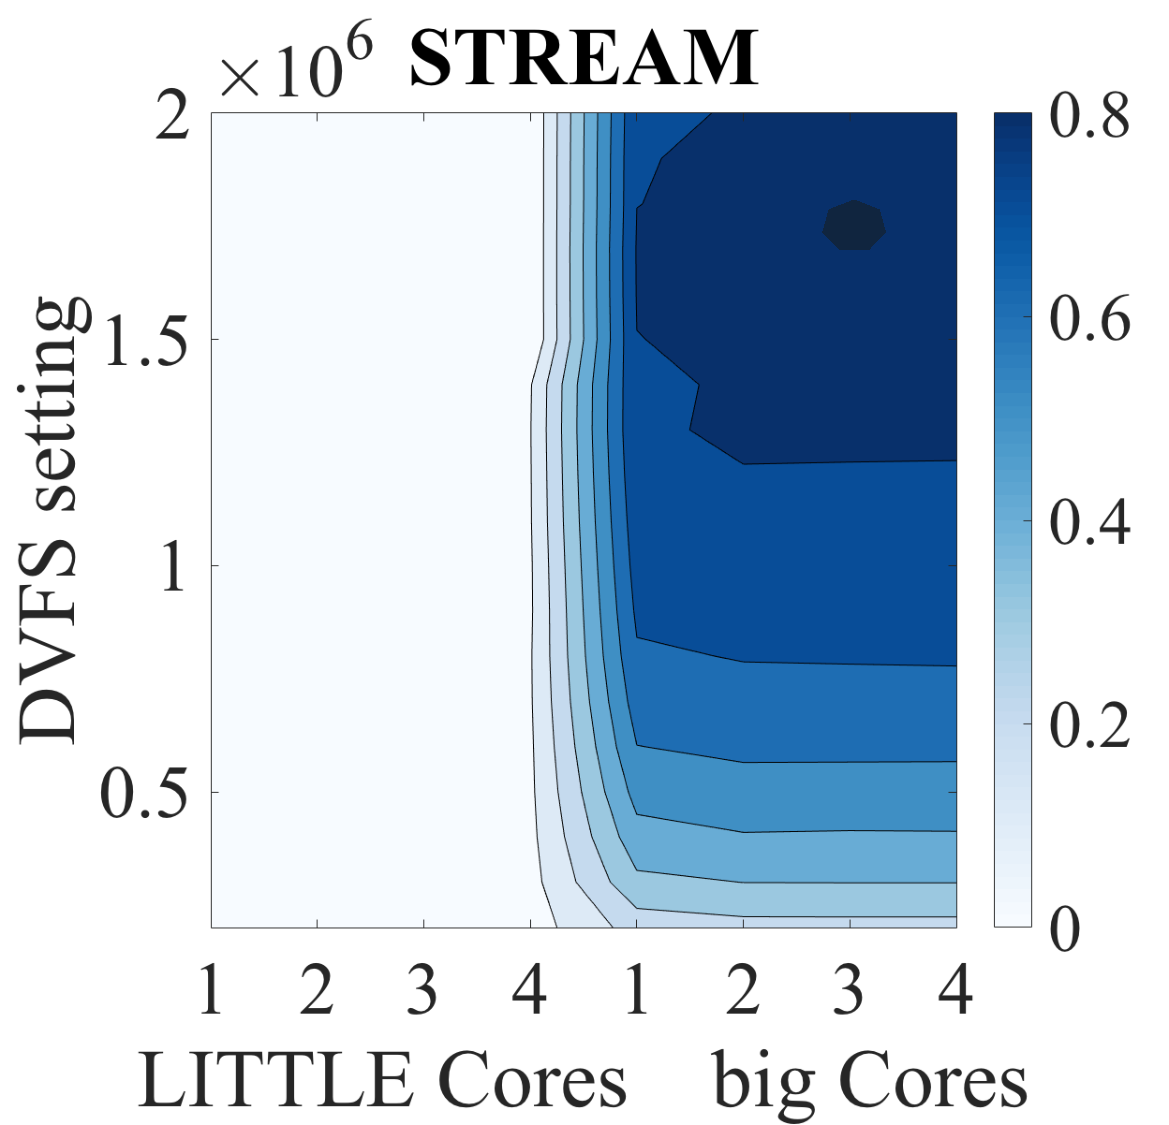
\includegraphics[width=.37 \textwidth]{figures/STREAM-contour.pdf}
    \label{fig:STREAM_contour}
    \begin{tikzpicture}
\begin{centering}

\definecolor{s1}{RGB}{228, 26, 28}
\definecolor{s2}{RGB}{55, 126, 184}
\definecolor{s3}{RGB}{77, 175, 74}
\definecolor{s4}{RGB}{152, 78, 163}
\definecolor{s5}{RGB}{255, 127, 0}

\begin{groupplot}[
    group style={
        group name=plots,
        group size=1 by 1,
        xlabels at=edge bottom,
        xticklabels at=edge bottom,
        vertical sep=5pt
    },
height=4.1cm,
width=0.45\columnwidth,
xmajorgrids,
ymajorgrids,
grid style={dashed},
xmax=20,
yticklabel pos=left,
enlargelimits=false,
tick align = outside,
tick style={white},
xticklabel shift={-5pt},
yticklabel shift={-5pt},
ylabel shift={-2pt},
ylabel style={align=center},
unbounded coords=jump,
]

\nextgroupplot[ylabel={\scriptsize Performance (Normalized)}, % Performance
xlabel={\footnotesize Iteration},
ymin=0,
ymax=1.5,
ytick={0.0,0.5,1.0,1.5},
yticklabels={,0.5,1.0,1.5},
legend entries={{\scriptsize $\mathsf{Performance Requirement}$},{\scriptsize $\mathsf{Learning}$},{\scriptsize $\mathsf{Adaptive Control}$},},
legend style={fill=none,draw=none,at={(0.5,1.5)},anchor=north,legend columns=1,line width=3pt},
]

\addplot[thick, solid, black] coordinates {(0,1) (20,1)};
\addplot[thick, solid, color=s4] table[x index=0,y index=1,col sep=space] {img/complexity-example-leo.txt};
\addplot[thick, solid, color=s5] table[x index=0,y index=1,col sep=space] {img/complexity-example-poet.txt};
\end{groupplot}
\end{centering}
\end{tikzpicture}
    \label{fig:STREAM_timeline}
  \caption{(a) \texttt{STREAM} performance as a function of
    configuration.  (b) Managing \texttt{STREAM}'s performance:
    \emph{Learning} handles the complex configuration space, but
    \emph{control} oscillates.}
  \label{fig:learning-models1}
\end{figure}

We demonstrate how well learning handles complex resource interaction
for \texttt{STREAM} on an ARM big.LITTLE processor with four big,
high-performance cores and four LITTLE, energy efficient cores.  The
big cores support 19 clock speeds, while the LITTLE cores support 14.


\figref{fig:learning-models1}a shows \texttt{STREAM}'s performance for
different resource configurations.  This memory-bound application has
complicated behavior: the LITTLE cores' memory hierarchy cannot
deliver the required performance.  The big cores' more powerful memory
system delivers much greater performance, but the peak occurs with 3
big cores.  Furthermore, at low clockspeeds, these 3 big cores cannot
saturate the memory bandwidth, while at high clockspeeds the
performance drops as the processor overheats, triggering thermal
management.  For \texttt{STREAM}, the peak speed occurs with 3 big
cores at 1.2 GHz, and it is not efficient to spend any time on the
LITTLE cores.  \texttt{STREAM}, however, does not have distinct
phases, so once a resource allocator finds the most energy efficient
configuration, it simply needs to maintain it.


\figref{fig:learning-models1}b shows 20 iterations of both learning
\cite{LEO} and adaptive control \cite{POET} allocating resources to
\texttt{STREAM}.  The x-axis shows iteration and the y-axis shows
performance normalized to the requirement.  The \emph{learning}
approach estimates \texttt{STREAM}'s performance and power for all
configurations and uses the lowest energy configuration that delivers
the required performance.  The \emph{adaptive controller} begins with
a generic model of power/performance tradeoffs.  As the controller
runs, it measures performance and adjusts both the allocated resources
and its own parameters using online measurements.  The adaptive
controller dynamically adjusts to non-linearities with a series of
linear approximations; however, it is sensitive to model inaccuracies,
which cause the oscillations that lead to performance violations.
This behavior occurs because the controller's adaptive mechanisms
cannot handle the STREAM's complexity, a known limitation of adaptive
control systems \cite{ControlWare,POET,ICSE2014}.  Hence, the
\emph{learner}'s ability to model complex behavior is crucial.

\subsection{\emph{Controlling} Dynamics}

\begin{figure}
\centering
    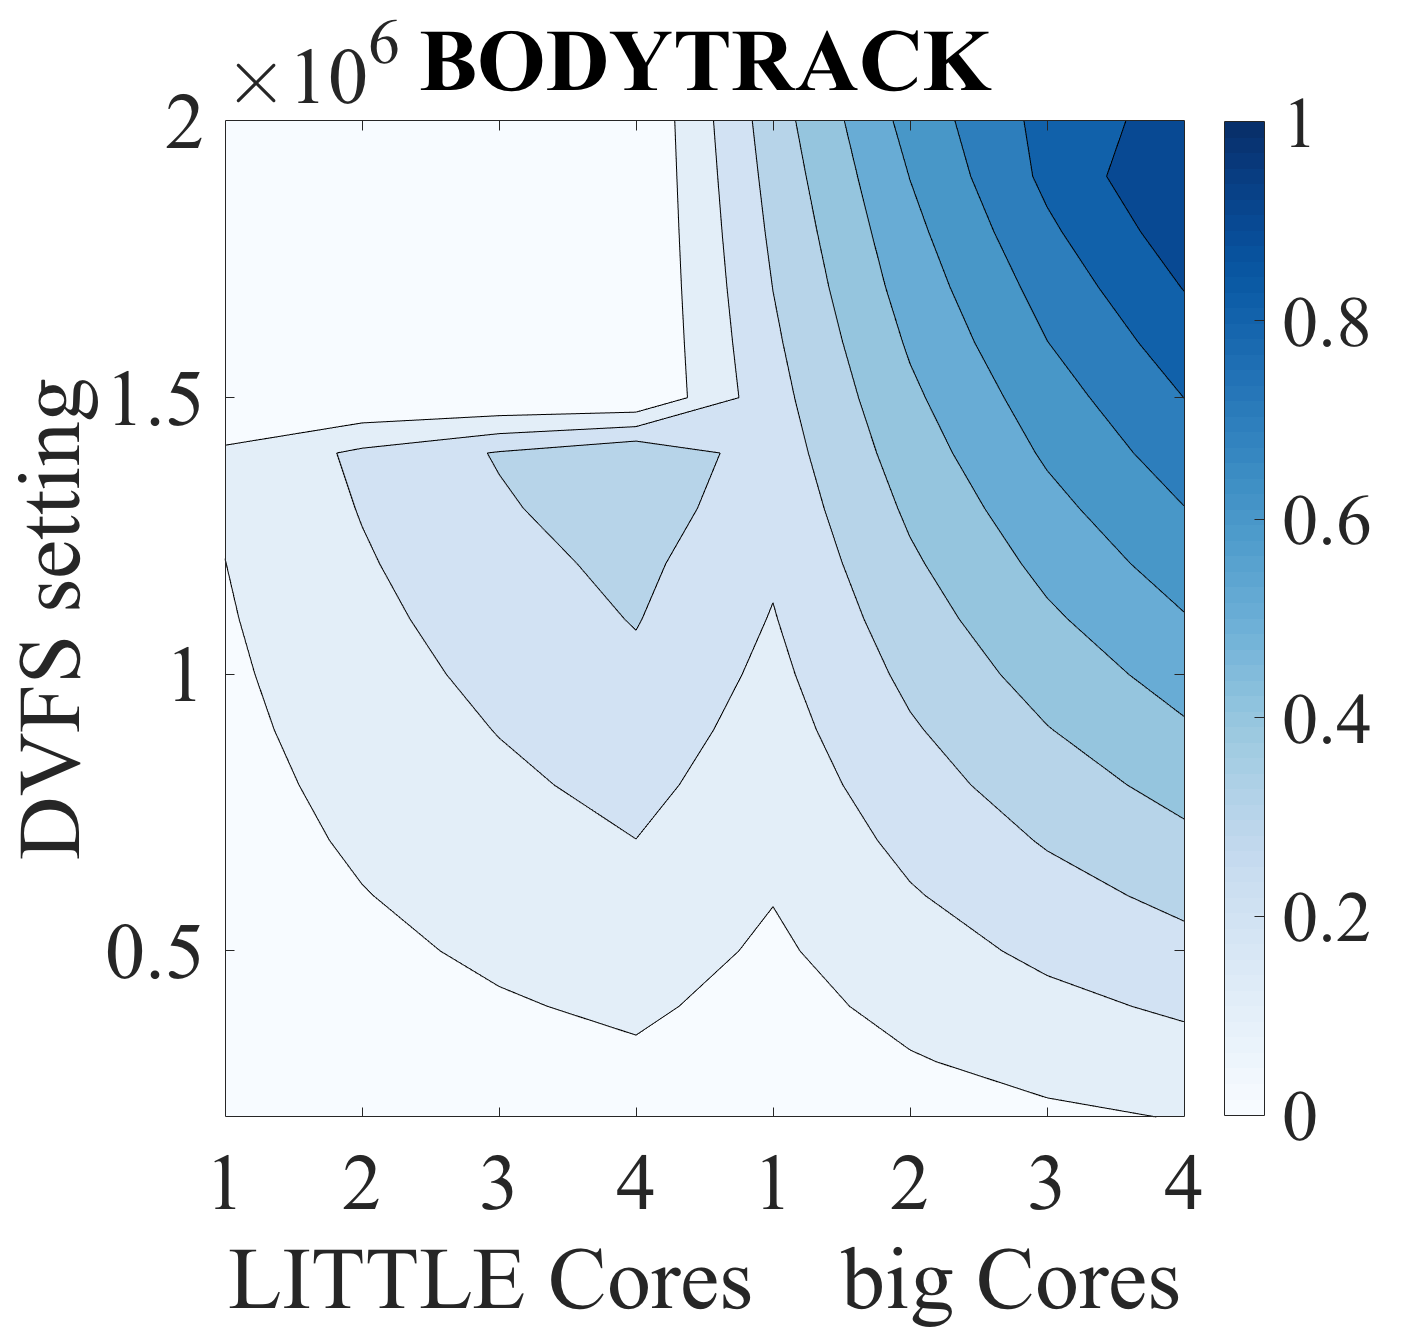
\includegraphics[width=.37\textwidth]{figures/BODYTRACK-contour.png}
    \label{fig:BODYTRACK_contour}
    \begin{tikzpicture}
\begin{centering}

\definecolor{s1}{RGB}{228, 26, 28}
\definecolor{s2}{RGB}{55, 126, 184}
\definecolor{s3}{RGB}{77, 175, 74}
\definecolor{s4}{RGB}{152, 78, 163}
\definecolor{s5}{RGB}{255, 127, 0}

\begin{groupplot}[
    group style={
        group name=plots,
        group size=1 by 1,
        xlabels at=edge bottom,
        xticklabels at=edge bottom,
        vertical sep=5pt
    },
height=4.1cm,
width=0.45\columnwidth,
xmajorgrids,
ymajorgrids,
grid style={dashed},
xmin=0,
xmax=20,
yticklabel pos=left,
enlargelimits=false,
tick align = outside,
tick style={white},
xticklabel shift={-5pt},
yticklabel shift={-5pt},
ylabel shift={-2pt},
ylabel style={align=center},
unbounded coords=jump,
]

\nextgroupplot[ylabel={\scriptsize Performance (Normalized)}, % Performance
%xtick={0,500,1000,1500,2000,2500,3000,3500,4000,4500},
ytick={0.0,0.5,1.0,1.5,2.0},
yticklabels={,0.5,1.0,1.5,2.0},
xtick={90,95,100,105,110},
xticklabels={90,95,100,105,110},
%yticklabel style={font=\footnotesize},
xlabel={\footnotesize frame},
xmin=90,
xmax=110,
ymin=0,
ymax=1.5,
legend entries={{\scriptsize $\mathsf{Performance Requirement}$},{\scriptsize $\mathsf{Learning}$},{\scriptsize $\mathsf{Adaptive Control}$}},
legend style={fill=none,draw=none,at={(0.5,1.5)},anchor=north,legend columns=1,
line width=5pt},
]

\addplot[thick, solid, black] coordinates {(0,1) (399,1)};
\addplot[thick, solid, color=s4] table[x index=0,y index=1,col sep=space] {img/dynamics-example-leo.txt};
\addplot[thick, solid, color=s5] table[x index=0,y index=1,col sep=space] {img/dynamics-example-poet.txt};
\addplot[thick, dashed, black] coordinates {(99,0) (99,1.5)};
%\addplot[thick, dashed, black] coordinates {(130,0) (130, 2)};
\end{groupplot}
\end{centering}

\end{tikzpicture}

    \label{fig:BODYTRACK_timeline}
  \caption{(a) \texttt{bodytrack} performance as a function of
    configuration. (b) Managing \texttt{bodytrack}'s performance with
    another application: \emph{control} detects the change (at the
    vertical dashed line) and adjusts, but \emph{learning} cannot. }
  \label{fig:control}
\end{figure}


We now consider a dynamic environment.  We begin with
\texttt{bodytrack} running alone on the system.  Halfway through its
execution, we launch a second application---\texttt{STREAM}---on a
single big core, dynamically changing available resources.
\figref{fig:control}a shows \texttt{bodytrack}'s behavior.
It achieves the best performance on 4 big cores at the highest
clockspeed; the 4 LITTLE are more energy-efficient but slower.  For
\texttt{bodytrack}, the challenge is determining how to split time
between the LITTLE and big cores to conserve energy while still
meeting the performance requirements.

\figref{fig:control}b shows the results of this experiment.
The vertical dashed line---at frame 99---represents when the second
application begins.  The figure clearly shows adaptive control's
benefits in this dynamic scenario.  When the second application
starts, the controller detects \texttt{bodytrack}'s performance
dip--rather than detecting the new application specifically---and it
changes resource allocation (increasing clockspeed and moving
bodytrack from 4 to 3 big cores).  The learning system however, does
not have any inherent mechanism to measure the change or adapt to the
altered performance.  While we could theoretically add feedback to the
learner and re-estimate the configuration space whenever the
environment changes, doing so is impractical due to high overhead for
learners capable of handling this complexity
\cite{Paragon,quasar,LEO}.


\subsection{Challenges of Parameter-free Control}
The adaptive controller requires user-specified parameters and
\figref{fig:not-simple} shows the consequences of getting those
parameters wrong. The controller's \emph{pole} is a particularly
important parameter.  Control engineers tune the pole with a model to
trade response time for noise sensitivity.  This model may be an
abstraction but is considered \emph{ground truth}
\cite{Hellerstein2004a}, meaning all possible resource configurations
the controller might select have been directly measured for some
input.  \SYSTEM{}, however, tunes the pole based on an estimated
model, which may have noise and/or errors.



%\begin{wrapfigure}{r}{0.5\columnwidth}
\begin{figure}
\centering
\begin{tikzpicture}
\begin{centering}

\definecolor{s1}{RGB}{228, 26, 28}
\definecolor{s2}{RGB}{55, 126, 184}
\definecolor{s3}{RGB}{77, 175, 74}
\definecolor{s4}{RGB}{152, 78, 163}
\definecolor{s5}{RGB}{255, 127, 0}

\begin{groupplot}[
    group style={
        group name=plots,
        group size=1 by 1,
        xlabels at=edge bottom,
        xticklabels at=edge bottom,
        vertical sep=5pt
    },
height=4.1cm,
width=0.45\columnwidth,
xmajorgrids,
ymajorgrids,
grid style={dashed},
xmin=0,
xmax=20,
yticklabel pos=left,
enlargelimits=false,
tick align = outside,
tick style={white},
xticklabel shift={-5pt},
yticklabel shift={-5pt},
ylabel shift={-2pt},
ylabel style={align=center},
unbounded coords=jump,
]

\nextgroupplot[ylabel={\scriptsize Performance (Normalized)}, % Performance
%xtick={0,500,1000,1500,2000,2500,3000,3500,4000,4500},
ytick={0.0,0.5,1.0,1.5,2.0},
yticklabels={,0.5,1.0,1.5,2.0},
xtick={90,95,100,105,110},
xticklabels={90,95,100,105,110},
%yticklabel style={font=\footnotesize},
xlabel={\footnotesize frame},
xmin=90,
xmax=110,
ymin=0,
ymax=1.5,
legend entries={{\scriptsize $\mathsf{Performance Requirement}$},{\scriptsize $\mathsf{Tuned Pole}$},{\scriptsize $\mathsf{Default Pole}$}},
legend style={fill=none,draw=none,at={(0.5,1.5)},anchor=north,legend columns=1,
line width=1pt},
]

\addplot[thick, solid, black] coordinates {(0,1) (399,1)};
\addplot[thick, solid, color=s5] table[x index=0,y index=1,col sep=space] {img/dynamics-example-poet.txt};
\addplot[thick, solid, color=s3] table[x index=0,y index=1,col sep=space] {img/dynamics-example-leopoetnp.txt};
\addplot[thick, dashed, black] coordinates {(99,0) (99,1.5)};
%\addplot[thick, dashed, black] coordinates {(130,0) (130, 2)};
\end{groupplot}
\end{centering}

\end{tikzpicture}

\caption{Comparison of carefully tuned and default poles.}
\label{fig:not-simple}
\end{figure}
%\end{wrapfigure}

To demonstrate the pole's importance when using a learned model, we
again control \texttt{bodytrack}, this time using the adaptive
controller from the previous subsection with a model produced by the
learner from the first subsection.  We compare the results with a
carefully tuned pole to those using the default pole provided by the
controller developers \cite{POET}.

\figref{fig:not-simple} shows the results.  The carefully tuned pole
converges because the pole accounts for the learned model's error. The
default pole, however, oscillates around the performance target,
resulting in a number of missed deadlines.  Additionally, the frames
that exceed the desired performance waste energy because they spend
more time on the big, inefficient cores. The pole parameterizes the
system's \emph{inertia}---dictating how fast it should react to
environmental changes.  If the estimated model is noisy, the
controller should trust it less and move slowly. Rather than require
users with both computing and control knowledge to tune the pole,
\emph{\SYSTEM{} incorporates the learner's confidence interval and
  estimated variance to compute a pole that provides probabilistic
  convergence guarantees.}

\section{\SYSTEM{}: Learning Control}
\label{sec:framework}

\begin{figure}
  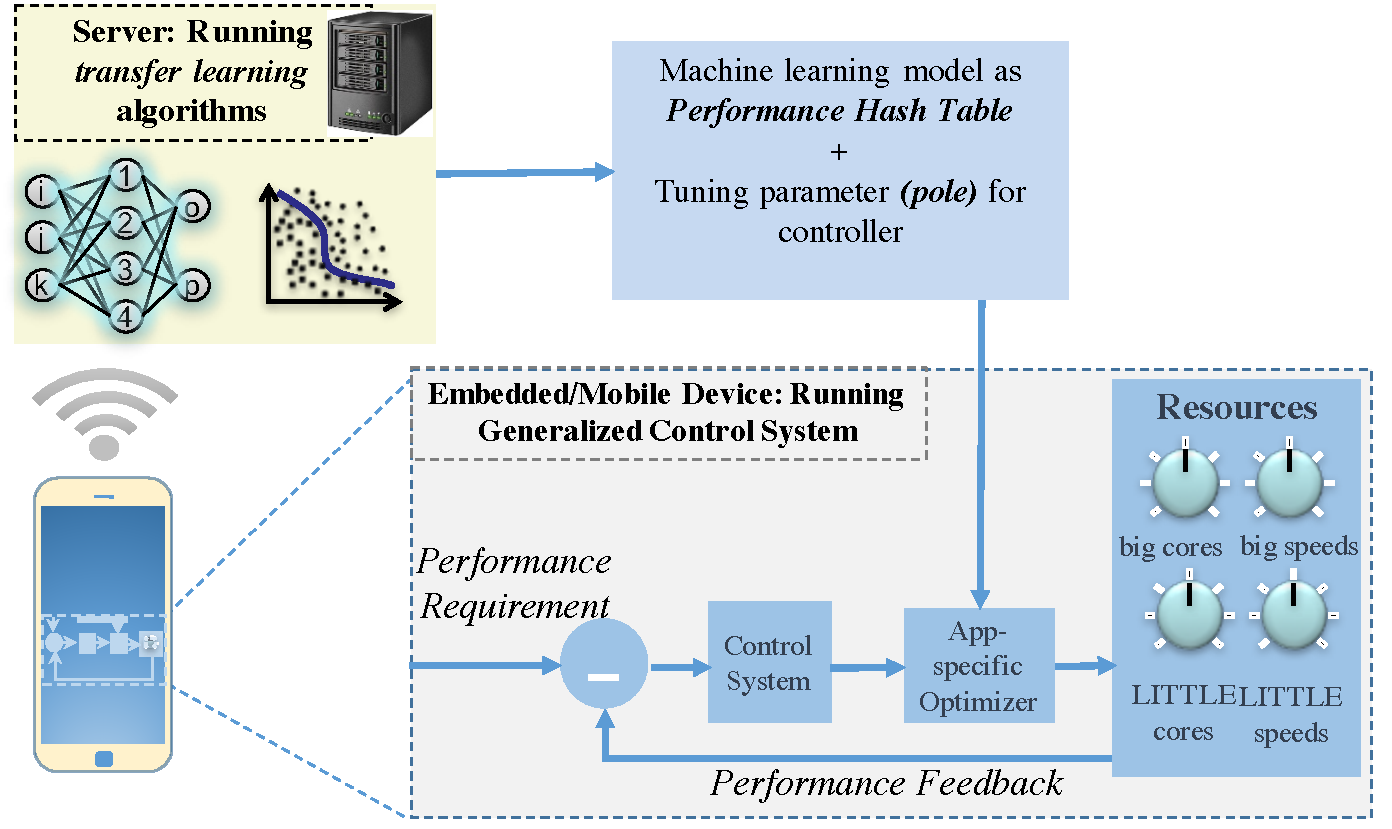
\includegraphics[width=\columnwidth]{figures/Overview.pdf}
  \caption{\SYSTEM{} overview.}
  \label{fig:overview}
\end{figure}


We describe \SYSTEM{}'s parameter-free resource management system,
which assumes no prior knowledge of the application and requires no
user-specified parameters.  \figref{fig:overview} shows \SYSTEM{}'s
approach.  A new application enters the system with a performance
requirement.  A generalized adaptive control system allocates
resources according to a generic model and records performance and
power.  The recorded values are sent to a learner, which estimates the
application's performance and power in all other configurations and
extracts those that represent Pareto-optimal tradeoffs.  These
configurations are packaged in a special data structure---the
performance hash table (PHT).  The learner sends the PHT and the
estimated variance to the controller.  Using these values, the
controller selects an energy minimal resource configuration in
constant time with formal guarantees of convergence to the desired
performance.

\begin{figure}
  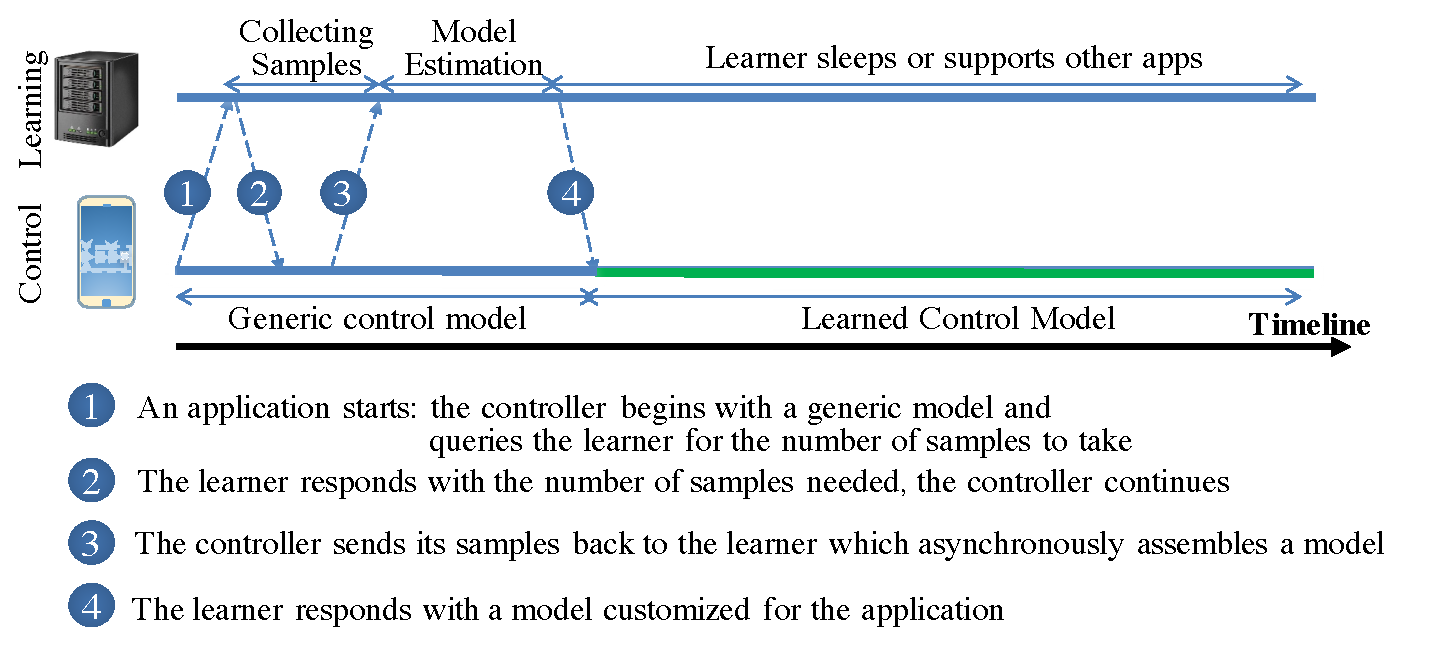
\includegraphics[width=\columnwidth]{figures/Timeline.pdf}
  \caption{Temporal relationship of learning and control.}
  \label{fig:timeline}
\end{figure}

\figref{fig:timeline} illustrates the asynchronous interaction between
\SYSTEM{}'s learner and controller over time. The controller starts
when a new application launches.  It has no prior knowledge of this
application, so it begins using a generic model.  At start, the
controller sends the learner the application name and device type
(message 1, \figref{fig:timeline}).  The learner determines how many
samples are needed for an accurate estimate and sends this number back
to the controller (message 2).  The controller takes these samples
while using the generic model and sends the learner the performance
and power of each measured configuration (message 3).  Computationally
expensive learners may require time to build a model.  Thus, the
controller does not wait for the learner, but continues with the
generic model.  Once the learner has a model and variance estimate, it
sends that data to the controller (message 4), which uses the learned
model from then on.

\figref{fig:timeline} shows several key points about the relationship
between learning and control.  First, the controller never waits for
the learner---it uses a generic model to provide less efficient
control until the learner can produce a customized model. Second, the
controller does not continuously communicate with the learner, this
interaction happens once at application launch.  Third, if the learner
crashed, the controller would just default to the behavior of a
generic adaptive control system.  If the learner crashed after
producing a model, control might not even need to know.  Finally,
because the learner and controller have a clearly defined interface,
they can be run in separate processes or physically separate devices.

This section first describes a traditional adaptive control system.
We then generalize this approach and separate out parameters to be
learned.  Next, we discuss the general class of learning systems that
work with \SYSTEM{}.  Then, we present an encoding for the learned
model that can be accessed by the controller in constant time.
Finally, we formally analyze \SYSTEM{}'s guarantees.


\subsection{Traditional Control for Computing}
Several researchers have proposed controlling computing systems.  A
controller that can manage multiple resources to meet multiple goals
is a multiple-input, multiple-output (MIMO) controller.  The inputs
are measurements, \eg{} performance.  The outputs are the resource
settings to be used at a particular time, \eg{} an allocation of big
and LITTLE cores and a clockspeed for each.

These difference equations describe a generic MIMO controller for
allocating $n$ resources to meet $m$ goals at time $t$:\footnote{We
  assume discrete time, and thus, use difference equations rather than
  differential equations that would be used for continuous systems.}
\begin{equation}
\begin{aligned}
&\x(t+1) &=& \mathbf{A} \cdot \x(t)& + \mathbf{B} \cdot \mathbf{c}(t)\\
&\y(t)   &=& \mathbf{C} \cdot \x(t)&,
\end{aligned}
\label{eqn:system:mimo}
\end{equation}
where $\x \in \R^{q}$ is the controller's \emph{state}, an abstract
representation of the relationship between resources and goals and $q$
is the controller's \emph{degree}, or complexity of its internal
state.  $\mathbf{c}(t) \in \R^n$ is a vector representing the current
\emph{configuration} of resources; \ie{} the $i$th vector element
represents the amount of resource $i$ to be allocated at time $t$.
$\y(t) \in \R^{m}$ represents the current value of the goal dimensions
at time $t$. The matrices $\mathbf{A} \in \R^{q \times q}$ and
$\mathbf{B} \in \R^{q \times n}$ relate the resource configuration to
the controller state.  The matrix $\mathbf{C} \in \R^{m \times q}$
relates the controller state to the expected behavior.  This model
does not assume the states or the resources are independent, but it
does assume that their relationship is linear.

For example, to allocate resources to meet performance goals in our
ARM big.LITTLE system---from \secref{example}---there are four
resources: the number of big cores, the number of LITTLE cores, and
the speeds for each of the big and LITTLE cores.  There is also a
single goal: performance.  Thus, in this example, $n=4$ and $m=1$. The
vector $\mathbf{c}(t)$ has four elements representing the resource
allocation at time $t$. $q$ is the number of variables in the
controller's state which can vary between, we can choose $q$ to be
between 1 to $n$.  The matrices $\mathbf{A}$, $\mathbf{B}$, and
$\mathbf{C}$ capture the linear relationship between the control state
$\x$, the resource usage $\mathbf{c}$, and the measured behavior.  In
this example, we know there is a non-linear relationship between the
resources.  We overcome this difficulty by tuning the identified
matrices at each time step---approximating the non-linear system
through a series of changing linear formulations.  This approximation
is a form of \emph{adaptive} or \emph{self-tuning} control
\cite{HandbookControl}.  Such adaptive controllers provide formal
guarantees that they will converge to the desired performance even in
the face of non-linearities, but they still assume convexity.

This control formulation has two major drawbacks.  First, because it
requires matrix computation, its overhead scales linearly in the
number of resources and in the number of goals
\cite{Hellerstein2004a,METE}.  Second, the adaptive mechanisms are not
parameter-free---they require users to specify starting values of the
matrices $\mathbf{A}$, $\mathbf{B}$, and $\mathbf{C}$ and the method
for updating these matrices to account for any non-convexity in the
relationship between resources and performance
\cite{POET,METE,ControlWare,HandbookControl}.  Therefore, typically
100s to 1000s of samples are taken at design time to ensure that the
starting matrices are sufficient to ensure convergence
\cite{FSE2015,sysid,josep-isca2016}.

\subsection{\SYSTEM{} Control System}
To overcome the above issues, \SYSTEM{} abstracts the controller of
\eqnref{system:mimo} and factors out those parameter to be learned.
Specifically, \SYSTEM{} takes three steps to transform a standard
control system into one that works without prior knowledge of the
application to be controlled:
\begin{enumerate}[leftmargin=1em]
\item controlling \emph{speedup} (which is an abstraction on performance) rather than resources,
\item translating speedup into an energy minimal \emph{resource
    schedule} in a separate step, and
\item exploiting the \emph{problem structure} to solve this scheduling
  problem in constant time.
\end{enumerate}
These steps assume a separate learner has produced a model of resource
performance and power.  The result is that \SYSTEM{}'s controller runs
in constant time without requiring any user-specified parameters.


% We first describe our formulation for controlling speedup and then
% converting that speedup into resource allocations.

\subsubsection{Controlling Speedup}
Instead of the matrix equations of \eqnref{system:mimo}, \SYSTEM{}
uses a scalar difference model relating speedup to performance:
\begin{equation}
  perf(t) = b(t) \cdot speedup(t-1) + \delta \label{eqn:speedup}
\end{equation}
where $b(t)$ is the application's \emph{base speed}: defined as the
speed when all resources are available.  While $b(t)$ is application
specific, it is easy to measure online, by simply allocating all
resources. Such a configuration should not violate any performance
constraints (although it is unlikely to be energy efficient) so it is
safe to take this measurement.  \SYSTEM{} assumes base speed is
time-variant as applications will transition through phases.

With this model, \SYSTEM{}'s control law is simply:
\begin{eqnarray}
  error(t) &=& goal - perf(t) \label{eqn:speedup-error} \\
  % speedup(t) &=& speedup(t-1) - \frac{error(t)}{b}
  speedup(t) &=& speedup(t-1) - \frac{1 - \rho(t)}{b(t)}.error(t)
  \label{eqn:speedup-control}
\end{eqnarray}
which states that the speedup at time $t$ is a function of the
previous speedup, the error at time $t$, the base speed $b(t)$, and
the controller's \emph{pole}, $\rho(t)$.  Standard control techniques
statically determine the pole and the base speed, but \SYSTEM{}
\emph{dynamically sets the pole and base speed to account for error in
  the learned models---an essential modification for providing formal
  guarantees of the combined control and learning systems.}  For
stable control, \SYSTEM{} ensures $0 \le \rho(t) < 1$. Small values of
$\rho(t)$ eliminate error quickly, but make the controller more
sensitive to model inaccuracies.  Larger $\rho(t)$ makes the system
more robust at the cost of reduced convergence time.  \SYSTEM{} sets
$b(t)$ using the standard technique of Kalman filter estimation
\cite{welch2006kalman}. \secref{guarantees} describes how \SYSTEM{}
automatically sets the pole; however, we first address converting an
abstract speedup into a resource allocation.

\subsubsection{Converting Speedup to Resource Schedules}
\SYSTEM{} must map \eqnref{speedup-control}'s speedup into a resource
allocation.  On our example ARM big.LITTLE architecture that means
mapping speedup into an allocation of big and LITTLE cores as well as
a speed for both (big and LITTLE cores are in separate clock domains).

The primary challenge is that speedups in real systems are discrete
non-linear functions of resource usage, while \eqnref{speedup-control}
is a continuous linear function.  We bridge this divide by assigning
time to resource allocations such that the average speedup over a
control interval is that produced by \eqnref{speedup-control}.

The assignment of time to resource configurations is a
\emph{schedule}; \eg{} spending 10 ms on the LITTLE cores at 0.6 GHz
and then 15 ms on the big cores at 1 GHz. Typically many schedules can
deliver a particular speedup and \SYSTEM{} must find one with minimal
energy.  Given a time interval $T$, the $speedup(t)$ from
\eqnref{speedup-control}, and $C$ different resource configurations,
\SYSTEM{} solves:
\begin{eqnarray}
  \minimize_{\mathbf{\tau} \in \R^{C}} && \sum_{c=0}^{C-1} \tau_c \cdot p_c \label{eqn:power}  \\
  \st %&& \nonumber\\
  && \sum_{c=0}^{C-1} \tau_c \cdot s_c =  speedup(t)T \label{eqn:work} \\
  && \sum_{c=0}^{C-1} \tau_c =  T \label{eqn:deadline} \\
  && 0 \le \tau_c \le T, \qquad \forall c \in \{0,\ldots,C-1\} \label{eqn:time}
\end{eqnarray}
where $p_c$ and $s_c$ are configuration $c$'s estimated
\emph{powerup}---analogous to speedup---and speedup; $\tau_c$ is the
time to spend in configuration $c$.  \eqnref{power} is the objective:
minimizing energy (power times time).  \eqnref{work} states that the
average speedup must be maintained, while \eqnref{deadline} requires
the time to be fully utilized.  \eqnref{time} simply avoids negative
time.

\subsection{Exploiting Structure for Fast Solutions}
%\SYSTEM{} solves \eqnrref{power}{time} on the local device (see
%\figref{fig:timeline}, so the solution must be efficient.
By exploiting the problem structure and encoding the learned model in
the performance hash table (PHT), \SYSTEM{} solves
\eqnrref{power}{time} in constant ($O(1)$) time.

Kim et al. analyze the problem of minimizing energy while meeting a
performance constraint and observe that there must be an optimal
solution with the following properties \cite{kim-cpsna}:
\begin{itemize}[leftmargin=1em]
\item At most two of $\tau_c$ are non-zero, meaning that at most two
  configurations will be used in any time interval.
\item If you chart the configurations in the power and performance
  tradeoff space (\eg{} the top half of \figref{fig:pht}) the two
  configurations with non-zero $\tau_c$ lie on the lower convex hull
  of the power performance tradeoff space.
\item The two configurations with non-zero $\tau_c$ are adjacent on
  the convex hull: one above the constraint and one below.
\end{itemize}
%\SYSTEM{} uses these two facts to construct a constant time algorithm
%for finding the optimal solution online.

\begin{figure}
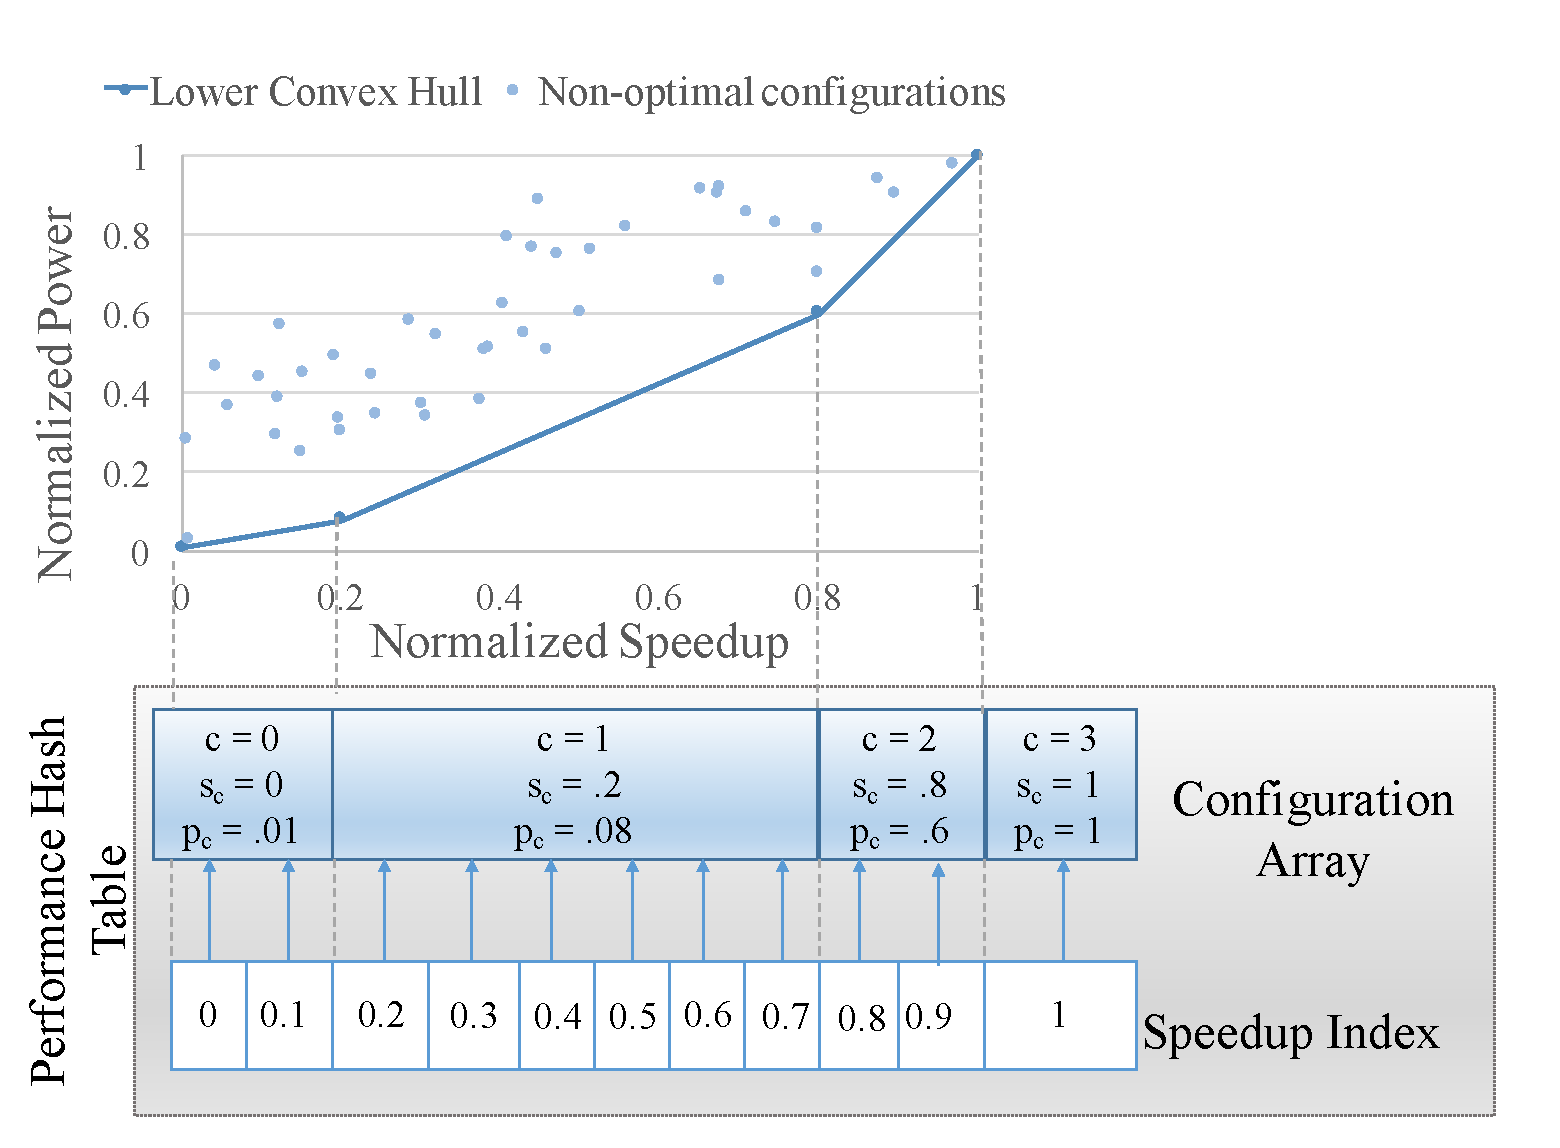
\includegraphics[width=\columnwidth]{figures/performance-hash-table.pdf}
\caption{Data structure to efficiently convert required speedup into a
  resource configuration.}
  \label{fig:pht}
\end{figure}

The PHT (shown in \figref{fig:pht}) provides constant time access to
points on the lower convex hull.  It consists of two arrays: the first
being pointers into the second, which stores resource configurations
on the lower convex hull sorted by speedup.  Recall speedups are
computed relative to the base speed, which uses all resources.  The
largest estimated speedup is therefore 1, so \SYSTEM{} needs only
consider speedups between 0 and 1.  The first array of pointers has a
\emph{resolution} indicating how many decimal points of precision it
captures and it is indexed by speedup.  The example in
\figref{fig:pht} has a resolution of $0.1$.  Each pointer in the first
array points to the configuration in the second array that has the
largest speedup less than or equal to the index.

\SYSTEM{} computes $speedup(t)$ and uses the PHT to convert speedup
into two configurations: $hi$ and $lo$.  To find the $hi$
configuration, \SYSTEM{} clamps the desired speedup to the largest
index lower than $speedup(t)$ and then walks forward until it finds
the first configuration with a speedup higher than $speedup(t)$.  To
find the $lo$ configuration, it clamps the desired speedup to the
smallest index higher than $speedup(t)$ and then walks backwards until
it finds the configuration with the largest speedup less than
$speedup(t)$.

For example, consider the PHT in \figref{fig:pht} and an optimizer
meeting $speedup(t) = .65$.  To find $hi$, the optimizer indexes at .6
and walks up to find $c=2$ with $s_c=.8$, setting $hi = 2$.  To find
$lo$, the optimizer indexes the table at .7 and walks backward to find
$c=1$ with $s_c=.2$, setting $lo = 1$.

\SYSTEM{} sets $\tau_{hi}$ and $\tau_{lo}$ by solving:
\begin{eqnarray}
  T &=& \tau_{hi} + \tau_{lo}    \label{eqn:s1} \\
  speedup(t) &=& \frac{s_{hi} \cdot \tau_{hi} + s_{lo} \cdot \tau_{lo}}{T} \label{eqn:s2}
\end{eqnarray}
where $speedup(t)$ is given by the controller and $s_c$ are speedups
estimated by the learner.  By solving \eqnsref{s1}{s2}, \SYSTEM{} has
turned the controller's speedup into a schedule of resource
allocations using learned models stored in the PHT.

\subsection{\SYSTEM{} Learning Algorithms}
The previous subsection describes a general control system, which can
be customized with a number of different learning methods.  The
requirements on the learner are that it must produce 1) estimates of
the speedup and powerup values for each resource configuration and 2)
an estimate of its own inaccuracy.
% We also provide a proxy for self tuning parameter in the later
% sections in case the learning algorithm cannot provide the
% confidence interval.
This section describes the general class of learning mechanisms that
meet these requirements.

When selecting a learning framework we must find a tradeoff between
the specific and the general; \ie between frameworks that build
application-specific models and frameworks that combine observations
across applications.  For example, the key to energy efficiency on
heterogeneous mobile systems is knowing when to make use of the
smaller, low-power cores \cite{kim-cpsna,Carroll2013,LeSueur11}.  An
application-specific model will capture that precisely, but may
require many observations before producing the correct model.  A more
general model will capture the trend, \eg when most applications
should transition, but this general model might miss the key
inflection point for some applications.  We refer to
application-specific models as \emph{online} because they build models
for the current application and do not incorporate knowledge of other
applications.  We refer to general models as \emph{offline} as they
use prior observations of other applications to predict the behavior
of a new application. A third class of \emph{transfer learning} models
combines information from the previously seen applications and current
application to make the predictions on the application in hand
\cite{pan2010survey} . These models allow us to obtain higher
prediction accuracies since we are able to augment our data with extra
information from other applications.

% The HBM provides a good balance between the online and offline
% approaches.  A strictly online approach will handle each new
% application completely separately and ignore observations of previous
% applications.  This approach never risks contaminating a model with
% unrelated observations, but it may take many observations of the
% current application to converge because it starts with no prior
% knowledge. The offline approach uses all observations from prior
% applications and will therefore converge very quickly; however, it is
% overly general and cannot learn features specific to a single
% application.
\subsubsection{Offline models}
These models utilize data from previously seen applications. If the
model is for applications with very similar behavior the prediction
accuracy might be high but the model will fail if the application's
behaviors diverge.  For example, these
techniques will predict the performance of applications based on prior
applications, meaning they will over-allocate speed to memory-bound
applications and under-allocate to compute-bound ones.

\subsubsection{Online models}
%\TODO{Is this offline or online or both?  The prior paragraph sets up this three-legged structure: offline, online, and something which we used to call hybrid but sounds like we are now calling transfer learning. If we are going to keep that structure we should mimic it in the substructure of the rest of the section.}
In general, all machine learning techniques take observations of some
phenomena and produce a model to estimate future outcomes.  In our
specific case, we want to take observations about application's
performance and power given a resource allocation and predict future
applications' behavior.  The most straightforward approach is to
create a linear regression model based on the configuration laid out
as the input features
\cite{tibshirani1996regression,yuan2006model,CPR}.  Learning in this
model requires samples of the performance and power for different
resource configurations.  Since the systems are usually non-linear,
polynomial regression models often give better results, but increases
the number of samples required to fit the model \cite{LeeBrooks}.
Regression models also provide a confidence interval for their
estimates which is important for adaptively tuning the pole.


\subsubsection{Transfer learning}
\textit{Transfer learning} refers to the process of applying knowledge
gained from one scenario to a new, similar one \cite{pan2010survey}.
To provide intuition we offer a simple example.  Suppose we have
observed many prior applications, all of which are either completely
compute-bound or completely memory-bound, and we have an equal number
of both.  The only resource we can allocate is clockspeed, which will
increase the performance of compute-bound applications, but not
memory-bound ones.  When we encounter new application, we must
estimate its response to clockspeed.  The online model will not use
prior knowledge, but will observe many different clock speeds for the
new application, leading to high overhead.  The offline model will
predict the mean response of prior applications, meaning it will
over-allocate speed to memory-bound applications and under-allocate to
compute-bound ones.  The transfer learning approach takes a small
number of samples and combines those with prior knowledge: if the new
observations show that clockspeed has no effect on performance these
models will use only the prior memory bound applications, otherwise,
it will use the compute-bound applications.

\paragraph{Netflix Algorithm:}
The Netflix problem is a famous challenge posted by Netflix to find
estimate users' movie preferences. The challenge was one by realizing
that if 2 users both like some movies they might have similar taste in
other movies. This approach allows allows models to borrow large
amounts of data from other users to answer some questions about a new
user.
%One of the solutions in designing this mathematically is to say
%the the matrix of users vs movies is low rank and solve the problem
%using mathematical optimization techniques.
Delimitriou and Kozyrakis use this algorithm to predict application
response to heterogeneous resources in data centers
\cite{Paragon,quasar}.


\paragraph{ Bayesian Models:} A hierarchical Bayesian model (HBM)
provides a statistically sound framework for learning across
applications and devices \cite{LEO}.  In the HBM, each application has
its own model, allowing specificity, but these models are
conditionally dependent on some underlying probability distribution
with a hidden mean and co-variance.  In practice, an HBM estimates a
model for a new application using a small number of observations and
combining those observations with the large number of previous
observations of other applications.  Rather than over-generalizing,
the HBM uses only similar applications to learn new models.  The HBM's
accuracy increases as more applications are observed because
increasingly diverse behaviors are represented in the pool of prior
knowledge.  Of course, the computational complexity of learning also
increases with increasing applications.


\subsection{Formal Analysis}
\subsubsection{Control System Complexity}
%\subsubsection{Algorithmic Analysis}

\SYSTEM{}'s control system (see Algorithm \ref{alg:gcs}) runs on the
local device along with the application under control, so its overhead
must be minimal.  In fact, each controller invocation is $O(1)$ .  The
only parts that are not obviously constant time are the PHT lookups.
Provided the PHT resolution is sufficiently high to avoid collisions,
then each PHT lookup requires constant time.
\begin{algorithm}[t]
\caption{\SYSTEM{} control.}
\label{alg:gcs}
\begin{algorithmic}
\REQUIRE Initialize the controller with a general model of speedup and powerup. Send power and performance samples to learner and receive a PHT.
\WHILE{$True$}
    \STATE    Measure streaming application performance
    \STATE    Compute required speedup (Equation \eqref{eqn:speedup})
    \STATE    Lookup $s_{hi}$ and $s_{lo}$ with PHT
    \STATE    Compute $\tau_{hi}$ and $\tau_{lo}$ (Equations \ref{eqn:s1} \& \ref{eqn:s2})
    \STATE    Configure to system to $hi$ $\&$ sleep $\tau_{hi}$.
    \STATE    Configure to $lo$ $\&$ sleep $\tau_{lo}$.
\ENDWHILE
\vskip -1.5em
\end{algorithmic}
\end{algorithm}

\subsubsection{Control Theoretic Formal Guarantees}
\label{sec:guarantees}
The controller's pole $\rho(t)$ is critical to providing control
theoretic guarantees in the presence of learned models.  \SYSTEM{}
requires any learner estimate not only speedup and powerup, but also
the variance $\sigma$.  \SYSTEM{} uses this information to derive a
lower bound for the pole which guarantees probabilistic convergence to
the desired performance. Specifically, we prove that with probability
99.7\% \SYSTEM{} converges to the desired performance if the pole is
$$\Floor{1- \Floor{max(\hat{s})/(min(\hat{s}) - 3\sigma)}_0}_0 \leq \rho(t)
< 1,$$ where $\Floor{x}_0 = \max(x,0)$ and $\hat{s}$ is the estimated
speedup. The appendix contains the proof. Users who need higher
confidence can set the scalar multiplier on $\sigma$ higher; \eg{}
using $6$ provides a 99.99966\% probability of convergence.

Thus we provide a lower-bound on the value of $\rho(t)$ required for a
user to be confident that \SYSTEM{} will converge to the desired
performance.  This pole value only considers performance, and not
energy efficiency.  In practice, we find that it better to use a
higher pole based on the \emph{uncertainty} between the controller's
observed energy efficiency and that predicted by the learned model.
We follow prior work in quantifying uncertainty as $\rho(t) $
\cite{Tokic2010}:
\begin{equation}
  \begin{array}{rcl}
    \beta(t) &=&  \text{exp}{\left(- \left( \left|   \frac{\bar{s}(t)}{\bar{p}(t)}  -\frac{ \hat{s}(t)}{\hat{p}_(t)} \right| \right) /5\right)} \\
    \rho(t) &=& \frac{1-\beta(t)}{1+\beta(t)}
  \end{array}
  \label{eqn:uncer}
\end{equation}
where $\bar{s}$ and $\bar{p}$ are the measured values of speedup and
power up and $\hat{s}$ and $\hat{p}$ are the estimated values from the
learner.  This measure of uncertainty captures both power and
performance.  We find that it is generally higher than the pole value
given by our lower bound, so in practice \SYSTEM{} sets the pole
dynamically to be the higher of the two values and \SYSTEM{} makes
spot updates to the estimated speedup and power based on its
observations.
\subsection*{Probabilistic Convergence Guarantees}


\begin{thm}
  Let $\mathbf{s}$ and $\hat{\mathbf{s}}$ denote the true and estimated speedups of various configurations in set $C$ as $\mathbf{s} \in \mathbb{R}^{|C|}$. Let $\sigma$ denote the
  estimation error for speedups such that, $\hat{s_i} \sim
  N(s_i, \sigma^2)$ $\forall$ $i$. We can show that with probability
  greater than 99.7\%, the pole $\rho(t)$ can be chosen to lie in the range, $[\Floor{1- \Floor{max(\hat{s})/(min(\hat{s}) -  3\sigma)}_0}_0, 1)$, where $\Floor{x}_0 = \max(x,0)$.
\end{thm}

\begin{proof}
Let $\Delta$ denote the multiplicative error over speedups, such that $ \widehat{speedup(t)}\Delta = speedup(t) $. To
guarantee convergence the value of pole, $\rho(t)$ can vary in the range
$\Floor{1-\frac{2}{\Delta})}_0, 1)$\cite{ICSE2014}. The lowest value of $\rho(t)$ offer the fastest convergence. We have described in Equations \ref{eqn:s1} \& \ref{eqn:s2} that any speedup can be written as a linear combination of two configuration speedups as,

\begin{align}
speedup(t) = \hat{s}_{hi} \cdot \tau_{hi} + \hat{s}_{lo} \cdot (T - \tau_{hi})
\end{align}
\begin{align}
\widehat{speedup}(t) = s_{hi} \cdot \tau_{hi} + s_{lo} \cdot (T - \tau_{hi})
\end{align}

We can upper bound and lower bound each of these terms,
\begin{align}
speedup(t) \leq T \hat{s}_{hi} \;\; \text{and} \;\; \widehat{speedup}(t) \geq T s_{lo}
\end{align}

The estimates of speedups are close to the actual speedups since
$\hat{s} \sim N(s, \sigma^2)$, therefore with probability greater
than 99.7\% and the speedups can be given by, $s_{lo} \geq
\hat{s}_{lo} - 3 \sigma$. Hence, $\widehat{speedup}(t) \geq T
(\hat{s}_{lo} -3 \sigma)$. Since, over all configurations, $\Delta \leq
\Floor{max(\hat{s})/(min(\hat{s}) - 3\sigma)}_0$,  we can choose the pole from the range,  $([\Floor{1- \Floor{max(\hat{s})/(min(\hat{s}) - 3\sigma)}_0}_0, 1)$.


\end{proof}

\section{Experimental Setup}
\begin{figure}[t]
  \subfloat[]
  {
    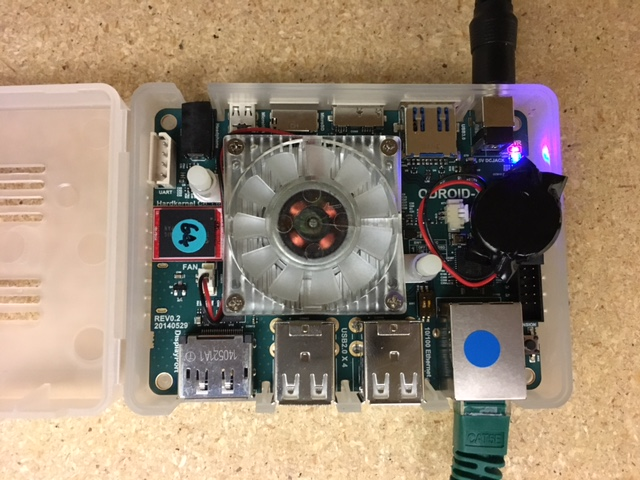
\includegraphics[width=.22\textwidth]{figures/odroid.png}
    \label{fig:odroid}
  }
  \subfloat[]
  {
    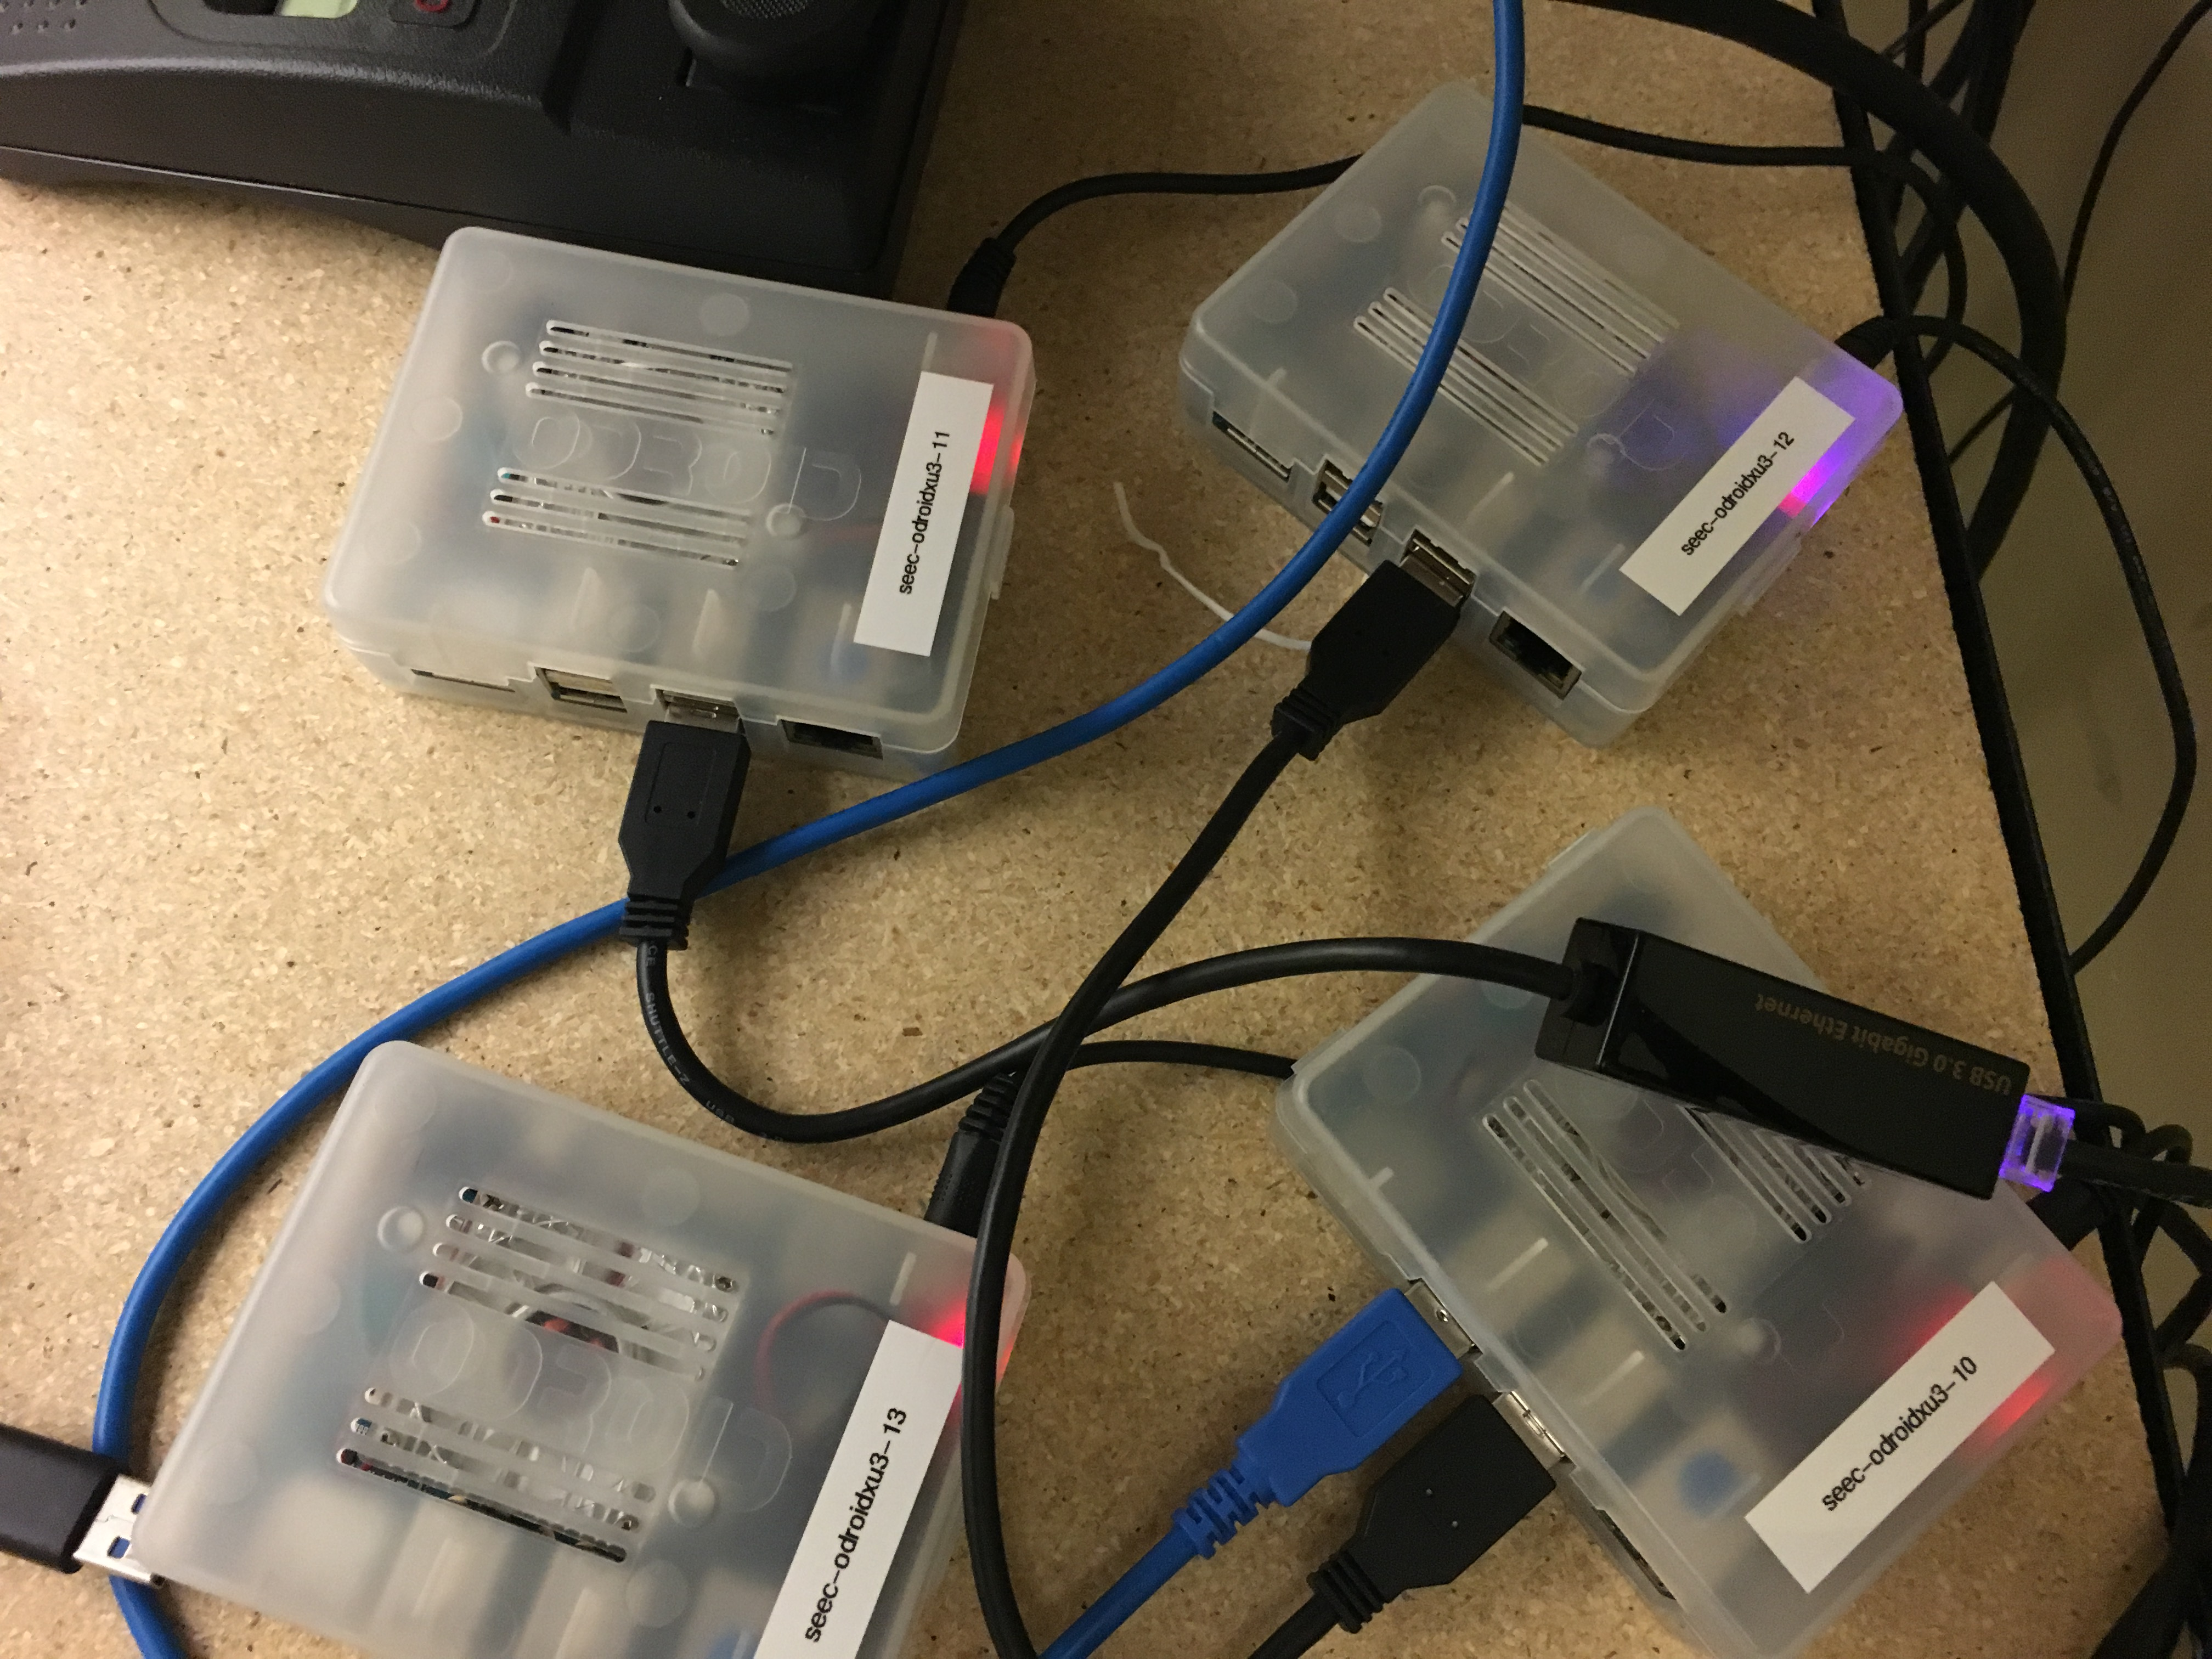
\includegraphics[width=.22\textwidth]{figures/odroidall.png}
    \label{fig:odroid_all}
  }
 \caption{ODROID-XU3 boards used in the evaluation.}
 \label{fig:odroidall}
\end{figure}

\subsection{Platform and Benchmarks}
We run streaming applications on four ODROID-XU3 devices running
Ubuntu 14.04, as shown in \figref{fig:odroidall}. The ODROIDs have
Samsung Exynos 5 Octa processors using the ARM big.LITTLE
architecture.  Each has 19 speed settings for the 4 big cores and 13
for 4 LITTLE cores.  Each board has an on-board power meter updated at
1/4 \ms intervals, this meter captures core, GPU, memory, and flash
drive power.  Each resource configuration (combination of big/LITTLE
cores and clock-speeds) has a different performance and power, which
is application-dependent.

We use 20 benchmarks from different suites including PARSEC
\cite{parsec}, Minebench \cite{minebench}, Rodinia \cite{rodinia}, and
STREAM \cite{stream}. \figref{fig:application_variety} shows the
variety of workloads indicated by the \emph{lack-of-fit} or the
absence of correlation between frequency and performance.
Applications with high lack-of-fit do not speed up with increasing
frequency---typical of memory bound applications. Applications with
low lack-of-fit do see increasing performance with increasing
clock-speed \cite{powerslope}.  Applications with intermediate
lack-of-fit tend to improve with increasing clock speed up to a point
and then see no further improvement.  Each application has an outer
loop which processes one unit in a data stream (\eg{} a point for
\texttt{kmeans} or a frame for \texttt{x264}). The application signals
the completion of processing a single stream element using a standard
API \cite{icac2010heartbeats}.  Performance targets are specified as
application-specific latencies for these stream elements.



\begin{figure}[t]
  \begin{tikzpicture}
\definecolor{s1}{RGB}{228, 26, 28}
\definecolor{s2}{RGB}{55, 126, 184}
\definecolor{s3}{RGB}{77, 175, 74}
\definecolor{s4}{RGB}{152, 78, 163}
\definecolor{s5}{RGB}{255, 127, 0}

\begin{groupplot}[
    group style={
        group name=plots,
        group size=1 by 1,
        xlabels at=edge top,
        xticklabels at=edge top,
        vertical sep=5pt
    },
axis x line* = top,
xlabel near ticks,
major x tick style = transparent,
height=6cm,
width=\columnwidth,
xmin=0,
xmax=9,
enlargelimits=false,
tick align = outside,
tick style={white},
ylabel style={align=center},
ytick=\empty,
xtick=\empty,
xticklabels={},
yticklabels={},
ymin=0,
ymax=1,
]
\nextgroupplot[ylabel={},
y label style={rotate=270},
ylabel shift={12mm},
]
\addplot[thick,solid, color=black] coordinates {(0,1) (22,1)};


\end{groupplot}

\begin{groupplot}[
    group style={
        group name=plots,
        group size=1 by 2,
        xlabels at=edge bottom,
        xticklabels at=edge bottom,
        vertical sep=5pt
    },
axis x line* = bottom,
xlabel near ticks,
major x tick style = transparent,
xlabel={},
height=3cm,
width=\columnwidth,
xmin=0,
xmax=21,
enlargelimits=false,
tick align = outside,
tick style={white},
ylabel style={align=center},
ytick=\empty,
ymin=0,
ymax=0.5,
ytick={0,0.1,0.3,0.5},
yticklabels={,0.1,0.3,0.5},
legend cell align=left,
legend style={ column sep=1ex },
ymajorgrids,
grid style={dashed},
]


\nextgroupplot[ybar=\pgflinewidth,
bar width=2.0pt,
ylabel={\footnotesize \emph{lack-of-fit} \\ (1-adjustedR2)},
ylabel shift={0mm},
xticklabel shift={1pt},
x tick label style={rotate=35, anchor=east},
xtick={1,2,3,4,5,6,7,8,9,10,11,12,13,14,15,16,17,18,19,20,21},
xticklabels={
{\scriptsize $\mathsf{backprop}$},
{\scriptsize $\mathsf{bfs}$},
{\scriptsize $\mathsf{blackscholes}$},
{\scriptsize $\mathsf{bodytrack}$},
{\scriptsize $\mathsf{facesim}$},
{\scriptsize $\mathsf{ferret}$},
{\scriptsize $\mathsf{heartwall}$},
{\scriptsize $\mathsf{hotspot}$},
{\scriptsize $\mathsf{jacobi}$},
{\scriptsize $\mathsf{kmeans}$},
{\scriptsize $\mathsf{kmeansnf}$},
{\scriptsize $\mathsf{lavamd}$},
{\scriptsize $\mathsf{leukocyte}$},
{\scriptsize $\mathsf{lud}$},
{\scriptsize $\mathsf{nw}$},
{\scriptsize $\mathsf{sha}$},
{\scriptsize $\mathsf{srad}$},
{\scriptsize $\mathsf{stream_threads}$},
{\scriptsize $\mathsf{x264-ducks}$},
{\scriptsize $\mathsf{x264-native}$}},
]
\addplot[color=calnp,fill=calnp] table[x index=0,y index=1, col sep=space] {img/image_text/mem-compute.txt};

\end{groupplot}
\end{tikzpicture}

   \vskip -1em
   \caption{\emph{Lack-of-fit} for performance vs clock-speed. Lower
     lack-of-fit indicates a more compute-bound application, higher
     values indicate a memory-bound one.}
  \label{fig:application_variety}
\end{figure}


\subsection{Evaluation Metrics}
%\SYSTEM{} uses the model for power and performance and its controller
%actively uses this knowledge to meet the performance target.
The latency targets represent performance requirements. To test a
variety of requirements, we run our applications with targets that
represent 50-90\% of the maximum speed and evaluate \SYSTEM{} under
each constraint. We quantify the performance reliability by measuring
the number of deadlines that were missed for each application and
performance target. If the application processes $n$ elements total
and $m$ of those elements took longer than the target latency we
compute deadline misses as:
\begin{equation}
deadline\, misses = 100\% \cdot \frac{m}{n}.
\end{equation}

We evaluate energy savings by constructing an oracle.  We run every
application in every resource configuration and record performance and
power for every stream element.  By post-processing this data we
determine the optimal resource configuration for each stream element
and performance target. To compare across applications, we normalize
energy:
\begin{equation}
  normalized\,energy = 100\% . \left( \frac{e_{measured}}{e_{optimal}} - 1 \right)
\end{equation}
where $e_{measured}$ is measured energy and $e_{optimal}$ is the
optimal energy produced by our oracle. We subtract 1, so that this
metric shows the percentage of energy over optimal.

\subsection{Points of Comparison}
We compare \SYSTEM{} to a number of existing learning and control
approaches:
\begin{enumerate}
\item \textit{Race-to-idle}: This well known heuristic allocates all
  resources to the application to complete each stream element as fast
  as possible, then idles until the next element is available
  \cite{kim-cpsna,powerslope,heisner}.  This heuristic requires no
  knowledge of the application and never misses deadlines in a
  single-application scenario.
\item \textit{PID-Control}: This is a standard single-input
  (performance), multiple-output (big/LITTLE core counts and speeds)
  proportional-integral-controller representative of several that have
  been proposed for computer resource management
  \cite{Hellerstein2004a,METE}.  This controller is tuned to provide
  the best average case behavior across all applications and targets.
\item \textit{Online}: observes the new application in small number of
  configurations then performs polynomial multivariate regression to
  estimate unobserved configurations' behavior
  \cite{LEO,Li2006,Ponamarev}.
\item \textit{Offline}: does not observe any values for the current
  application---instead using previously observed applications to
  estimate power and performance as a linear regression.  This
  baseline represents the class learners that build models with a
  training set and apply them without new observations
  \cite{PUPiL,LeeBrooks2006,CPR}.
\item \textit{Netflix}: is a matrix completion algorithm for the
  Netflix challenge. Variations of this approach allocate
  heterogeneous resources in data centers \cite{Paragon,quasar}.
\item \textit{HBM}: is a hierarchical Bayesian learner previously used
  to allocate resources to meet performance goals with minimal energy
  in server systems \cite{LEO}.
\item \textit{Adaptive-Control}: is a state-of-the-art, adaptive
  controller that meets application performance with minimal energy
  \cite{POET}.  This approach requires a user-specified starting
  model, we use the model produced by the \emph{Offline} learner. A
  recent study comparing ML and control techniques for resource
  allocation showed that there was no single best approach, but
  adaptive control had the best average behavior \cite{TAAS}.
\end{enumerate}


\SYSTEM{} is a framework for combining different learners with the
\SYSTEM{} control system.  We compare the above baselines to four
different versions of \SYSTEM{}:
\begin{enumerate}
\item \textit{CALOREE-NoPole}: uses the HBM learner, but sets the pole
  set to 0.  This baseline shows the importance of incorporating the
  confidence interval and model variance into control. All other
  versions of \SYSTEM{} set the pole according to \secref{guarantees}.
\item \textit{CALOREE-online}: uses the online learner.
\item \textit{CALOREE-nuclear}: uses the Nuclear learner.
\item \textit{CALOREE-HBM}: uses the HBM learner.
\end{enumerate}

In all cases that require prior knowledge, we ensure that knowledge of
the application under test is never included in that set of prior
knowledge.  Specifically, we use leave-one-out cross validation: to
test application $x$, we form a set of all other applications, train
the models, and then test on $x$.

\section{Experimental Evaluation}

\subsection{Performance and Energy for Single App}
%Setup

\begin{figure}[!th]
\centering
  \begin{tikzpicture}
\begin{centering}
\pgfplotstableread[col sep=space]{img/single-eff-summary.txt}{\datatableeff}
\pgfplotstableread[col sep=space]{img/single-lat-summary.txt}{\datatablelat}
\begin{groupplot}[
% MAKE SURE NO SPACE AROUND EQUALITY
    scatter/classes={
            OPTIMAL={mark=otimes*,OPTIMAL},
            RACE={mark=otimes*,RACE},
            CONTROL={mark=otimes*,CONTROL},
            ONLINE={mark=otimes*,ONLINE},
            OFFLINE={mark=otimes*,OFFLINE},
            NUCLEAR={mark=otimes*,NUCLEAR},
            HBM={mark=otimes*,HBM},
            ADAPT-CONTROL={mark=otimes*,ADAPT-CONTROL},
            CALOREE-NP={mark=otimes*,CALOREE-NP},
            ONLINE-ADAPT={mark=otimes*,ONLINE-ADAPT},
            NUCLEAR-ADAPT={mark=otimes*,NUCLEAR-ADAPT},
            HBM-ADAPT={mark=otimes*,HBM-ADAPT}},
    group style={
        group name=plots,
        group size=1 by 2,
        xlabels at=edge bottom,
        xticklabels at=edge bottom,
        vertical sep=5pt},
    enlargelimits=false,
    tick align = outside,
    tick style={white},
    ylabel style={align=center},
    unbounded coords=jump,
    grid=both,
]

\nextgroupplot[
        scale only axis,
        height=2cm,
        width=0.80\columnwidth,
        xlabel near ticks,
        xlabel = {},
        xmin = 0,
        xmax = 13,
        xtick={1,2,3,4,5,6,7,8,9,10,11,12,13},
        x tick label style={rotate=45, anchor = east, font=\tiny},
        ylabel={\tiny Deadline Misses (\%) \\ {\tiny (lower is better)}},    
        ytick pos=left
        ]
        \addplot[scatter, only marks ,thick, scatter src=explicit symbolic] table[x index=0,y index=3, meta=Benchmark] {\datatablelat};
        %\addplot[only marks, mark=diamond*, scatter src=explicit symbolic,  error bars/.cd, y dir=minus,  y explicit ] table [x index=0, y index=3, y error index=2, meta=Benchmark]  {\datatable};
        \addplot[only marks,mark=o,  scatter src=explicit symbolic,  error bars/.cd, y dir=plus,   y explicit] table [x index=0, y index=3, y error index=4, meta=Benchmark]  {\datatablelat};
        \addplot[only marks, mark=o, scatter src=explicit symbolic,  error bars/.cd, y dir=minus,  y explicit ] table [x index=0, y index=3, y error index=2, meta=Benchmark]  {\datatablelat};

\nextgroupplot[
        scale only axis,
        %grid=both,
        height=2cm,
        width=0.80\columnwidth,
        xlabel near ticks,
        xlabel = {},
        xmin = 0,
        xmax = 13,
        ylabel={\tiny Energy Over Optimal (\%) \\ {\tiny (lower is better)}},
        xticklabel shift={0pt},
        xtick={1,2,3,4,5,6,7,8,9,10,11,12,13},
        x tick label style={rotate=45, anchor = east, font=\tiny},
        %xticklabels from table={\datatableeff}{Benchmark},
        xticklabels={{\scriptsize $\mathsf{Optimal}$},
{\scriptsize $\mathsf{Race-to-idle}$},
{\scriptsize $\mathsf{PID-Control}$},
{\scriptsize $\mathsf{Online}$},
{\scriptsize $\mathsf{Offline}$},
{\scriptsize $\mathsf{Netflix}$},
{\scriptsize $\mathsf{HBM}$},
{\scriptsize $\mathsf{Adaptive-Control}$},
{\scriptsize $\mathsf{CALOREE-NoPole}$},
{\scriptsize $\mathsf{CALOREE-Online}$},
{\scriptsize $\mathsf{CALOREE-Netflix}$},
{\scriptsize $\mathsf{CALOREE-HBM}$}
},
]

        ]
        \addplot[scatter, only marks ,thick, scatter src=explicit symbolic] table[x index=0,y index=3, meta=Benchmark] {\datatableeff};
        \addplot[only marks,mark=o,  scatter src=explicit symbolic,  error bars/.cd, y dir=plus,   y explicit] table [x index=0, y index=3, y error index=2]  {\datatableeff};
        \addplot[only marks, mark=o, scatter src=explicit symbolic,  error bars/.cd, y dir=minus,  y explicit] table [x index=0, y index=3, y error index=4]  {\datatableeff};

\end{groupplot}
\end{centering}
\end{tikzpicture}

   \vskip -.5em
  \caption{Summary data for single-app scenario.}
  \label{fig:single-sum}
\end{figure}

We set a range of performance targets from 50-90\% of the maximum
achievable performance and measure the deadline misses and
energy over optimal for all points of comparison.
\figref{fig:single-sum} represents the summary results as an average
error across all targets for the single application scenario. This figure
shows two charts with the percentage of deadline misses in the top
chart and the energy over optimal in the bottom.  The dots show the
average for each technique, while the error bars show the minimum and
maximum values.

Not surprisingly, race-to-idle meets all deadlines, but its
conservative resource allocation has the highest average energy
consumption. Among the prior learning approaches Nuclear has the
lowest average deadline misses (11\%), but with high energy (40\% more
than optimal), while the HBM has higher deadline misses (17\%) but
with significantly lower energy consumption (16\%). Adaptive control
achieves similar deadline misses (14\%) with lower average energy than
any of the prior learning approaches (12\%). \SYSTEM{} with no pole
misses 45\% of all deadlines, which is clearly unacceptable.


\begin{figure*}[t]
 \captionsetup[subfigure]{labelformat=empty}
  \subfloat[]
  {
    \begin{tikzpicture}
%\pgfplotstableread[col sep=space]{img/image_text/dyn-mape-0.5-v2.txt}{\datatablefive}
\pgfplotstableread[col sep=space]{img/image_text/dyn-lat-0.60-v3.txt}{\datatablesixty}
\pgfplotstableread[col sep=space]{img/image_text/dyn-lat-0.75-v3.txt}{\datatableseventyfive}
\pgfplotstableread[col sep=space]{img/image_text/dyn-lat-0.90-v3.txt}{\datatableninty}
\begin{groupplot}[
    group style={
        group name=plots,
        group size=1 by 3,
        xlabels at=edge bottom,
        xticklabels at=edge bottom,
        vertical sep=5pt
    },
axis x line* = bottom,
xlabel near ticks,
major x tick style = transparent,
xlabel={},
height=2.8cm,
width=0.88\textwidth,
xmin=0,
xmax=23,
enlargelimits=false,
tick align = outside,
tick style={white},
ylabel style={align=center},
ytick=\empty,
ymin=0,
ymax=30,
ytick={0,5,10,15,20},
yticklabels={,5,10,15,20},
legend cell align=left, 
legend style={ column sep=1ex },
ymajorgrids,
grid style={dashed},
]


\nextgroupplot[ybar=\pgflinewidth,
ylabel shift={0mm},
bar width=2.0pt,
legend entries = {{$\mathsf{Race-to-idle}$},
{$\mathsf{Netflix}$},
{$\mathsf{HBM}$},
{$\mathsf{Adaptive-Control}$},
{$\mathsf{CALOREE-HBM}$}},
legend style={draw=none, legend columns=6,at={(.5,1.7)},anchor=north},
ymin=0,
ymax=20,
ytick={0.0,5.0,10.0,15.0,20.0},
yticklabels={,5.0,10.0,15.0},
]

\addplot[color=RACE, fill=RACE]       table[x index=0,y index=3] {\datatablesixty};
\addplot[color=NETFLIX, fill=NETFLIX]     table[x index=0,y index=6] {\datatablesixty};
\addplot[color=HBM, fill=HBM]   table[x index=0,y index=7] {\datatablesixty};
\addplot[color=POET, fill=POET] table[x index=0,y index=9] {\datatablesixty};
\addplot[color=CALOREE-HBM, fill=CALOREE-HBM]     table[x index=0,y index=13] {\datatablesixty};
                                

\nextgroupplot[ybar=\pgflinewidth,
ylabel={\footnotesize Deadline Misses (\%)  {\scriptsize (lower is better)}},
ylabel shift={0mm},
bar width=2.0pt,
ymin=0,
ymax=30,
ytick={0.0,10.0,20.0,30.0},
yticklabels={,10.0,20.0,30.0},
]

%\addplot[color=RACE,fill=RACE] table[x index=0,y index=4] {\datatableseventyfive};
%\addplot[color=HBM,fill=HBM]       table[x index=0,y index=7] {\datatableseventyfive};
%\addplot[color=ADAPT-CONTROL,fill=ADAPT-CONTROL] table[x index=0,y index=9] {\datatableseventyfive};
%\addplot[color=CALOREE-NP,fill=CALOREE-NP]   table[x index=0,y index=10] {\datatableseventyfive};
%\addplot[color=HBM-ADAPT,fill=HBM-ADAPT]       table[x index=0,y index=13] {\datatableseventyfive};
\addplot[color=RACE, fill=RACE]       table[x index=0,y index=3] {\datatableseventyfive};
\addplot[color=NETFLIX, fill=NETFLIX]     table[x index=0,y index=6] {\datatableseventyfive};
\addplot[color=HBM, fill=HBM]   table[x index=0,y index=7] {\datatableseventyfive};
\addplot[color=POET, fill=POET] table[x index=0,y index=9] {\datatableseventyfive};
\addplot[color=CALOREE-HBM, fill=CALOREE-HBM]     table[x index=0,y index=13] {\datatableseventyfive};

\nextgroupplot[ybar=\pgflinewidth,
bar width=2.0pt,
ylabel shift={0mm},
xticklabel shift={0pt},
ymin=0,
ymax=30,
ytick={0.0,10.0,20.0,30.0},
yticklabels={,10.0,20.0,30.0},
x tick label style={rotate=35, anchor=east},
xtick={1,2,3,4,5,6,7,8,9,10,11,12,13,14,15,16,17,18,19,20,21,22},
xticklabels={},
]

\addplot[color=RACE, fill=RACE]       table[x index=0,y index=3] {\datatableninty};
\addplot[color=NETFLIX, fill=NETFLIX]     table[x index=0,y index=6] {\datatableninty};
\addplot[color=HBM, fill=HBM]   table[x index=0,y index=7] {\datatableninty};
\addplot[color=POET, fill=POET] table[x index=0,y index=9] {\datatableninty};
\addplot[color=CALOREE-HBM, fill=CALOREE-HBM]     table[x index=0,y index=13] {\datatableninty};

\end{groupplot}
\begin{groupplot}[
    group style={
        group name=plots,
        group size=1 by 6,
        xlabels at=edge top,
        xticklabels at=edge top,
        vertical sep=5pt
    },
axis x line* = top,
xlabel near ticks,
major x tick style = transparent,
height=2.8cm,
width=0.88\textwidth,
xmin=0,
xmax=9,
enlargelimits=false,
tick align = outside,
tick style={white},
ylabel style={align=center},
ytick=\empty,
xtick=\empty,
xticklabels={},
yticklabels={},
ymin=0,
ymax=1,
]

\nextgroupplot[
ylabel shift={12mm},
ylabel style={rotate=270},
ylabel={$\mathsf{60\%}$},
]
\addplot[thick,solid, color=black] coordinates {(0,1) (22,1)};


\nextgroupplot[
ylabel shift={12mm},
ylabel={$\mathsf{75\%}$},
ylabel style={rotate=270},
]
\addplot[thick,solid, color=black] coordinates {(0,1) (22,1)};


\nextgroupplot[
ylabel shift={12mm},
ylabel={$\mathsf{90\%}$},
y label style={rotate=270},
]
\addplot[thick,solid, color=black] coordinates {(0,1) (22,1)};

\end{groupplot}

\end{tikzpicture}

  }
  \\
  \vskip -2.5em
  \subfloat[]
  {
    \begin{tikzpicture}

\pgfplotstableread[col sep=space]{img/image_text/dyn-eff-0.60-v3.txt}{\datatablesixty}
\pgfplotstableread[col sep=space]{img/image_text/dyn-eff-0.75-v3.txt}{\datatableseventyfive}
\pgfplotstableread[col sep=space]{img/image_text/dyn-eff-0.90-v3.txt}{\datatableninty}
\begin{groupplot}[
    group style={
        group name=plots,
        group size=1 by 3,
        xlabels at=edge bottom,
        xticklabels at=edge bottom,
        vertical sep=5pt
    },
axis x line* = bottom,
xlabel near ticks,
major x tick style = transparent,
xlabel={},
height=2.8cm,
width=0.88\textwidth,
xmin=0,
xmax=23,
enlargelimits=false,
tick align = outside,
tick style={white},
ylabel style={align=center},
ytick=\empty,
ymin=0,
ymax=30,
ytick={0,5,10,15,20},
yticklabels={,5,10,15,20},
legend cell align=left, 
legend style={ column sep=1ex },
ymajorgrids,
grid style={dashed},
]


\nextgroupplot[ybar=\pgflinewidth,
ylabel shift={0mm},
bar width=2.0pt,
ymin=0,
ymax=90,
ytick={0.0,30.0,60.0,90.0},
yticklabels={,30.0,60.0,90.0},
]

\addplot[color=RACE, fill=RACE]       table[x index=0,y index=3] {\datatablesixty};
\addplot[color=NETFLIX, fill=NETFLIX]     table[x index=0,y index=6] {\datatablesixty};
\addplot[color=HBM, fill=HBM]   table[x index=0,y index=7] {\datatablesixty};
\addplot[color=POET, fill=POET] table[x index=0,y index=9] {\datatablesixty};
\addplot[color=CALOREE-HBM, fill=CALOREE-HBM]     table[x index=0,y index=13] {\datatablesixty};
                                

\nextgroupplot[ybar=\pgflinewidth,
ylabel={\footnotesize Energy Above Optimal  {\scriptsize (lower is better)}},
ylabel shift={0mm},
bar width=2.0pt,
ymin=0,
ymax=90,
ytick={0.0,30.0,60.0,90.0},
yticklabels={,30.0,60.0,90.0},]

%\addplot[color=RACE,fill=RACE] table[x index=0,y index=4] {\datatableseventyfive};
%\addplot[color=HBM,fill=HBM]       table[x index=0,y index=7] {\datatableseventyfive};
%\addplot[color=ADAPT-CONTROL,fill=ADAPT-CONTROL] table[x index=0,y index=9] {\datatableseventyfive};
%\addplot[color=CALOREE-NP,fill=CALOREE-NP]   table[x index=0,y index=10] {\datatableseventyfive};
%\addplot[color=HBM-ADAPT,fill=HBM-ADAPT]       table[x index=0,y index=13] {\datatableseventyfive};
\addplot[color=RACE, fill=RACE]       table[x index=0,y index=3] {\datatableseventyfive};
\addplot[color=NETFLIX, fill=NETFLIX]     table[x index=0,y index=6] {\datatableseventyfive};
\addplot[color=HBM, fill=HBM]   table[x index=0,y index=7] {\datatableseventyfive};
\addplot[color=POET, fill=POET] table[x index=0,y index=9] {\datatableseventyfive};
\addplot[color=CALOREE-HBM, fill=CALOREE-HBM]     table[x index=0,y index=13] {\datatableseventyfive};

\nextgroupplot[ybar=\pgflinewidth,
bar width=2.0pt,
ylabel shift={0mm},
xticklabel shift={0pt},
ymin=0,
ymax=90,
ytick={0.0,30.0,60.0,90.0},
yticklabels={,30.0,60.0,90.0},
x tick label style={rotate=35, anchor=east},
xtick={1,2,3,4,5,6,7,8,9,10,11,12,13,14,15,16,17,18,19,20,21,22},
xticklabels={
{\scriptsize $\mathsf{backprop}$},
{\scriptsize $\mathsf{bfs}$},
{\scriptsize $\mathsf{blackscholes}$},
{\scriptsize $\mathsf{bodytrack}$},
{\scriptsize $\mathsf{facesim}$},
{\scriptsize $\mathsf{ferret}$},
{\scriptsize $\mathsf{heartwall}$},
{\scriptsize $\mathsf{hotspot}$},
{\scriptsize $\mathsf{jacobi}$},
{\scriptsize $\mathsf{kmeans}$},
{\scriptsize $\mathsf{kmeansnf}$},
{\scriptsize $\mathsf{lavamd}$},
{\scriptsize $\mathsf{leukocyte}$},
{\scriptsize $\mathsf{lud}$},
{\scriptsize $\mathsf{nw}$},
{\scriptsize $\mathsf{sha}$},
{\scriptsize $\mathsf{srad}$},
{\scriptsize $\mathsf{stream}$},
{\scriptsize $\mathsf{stream_threads}$},
{\scriptsize $\mathsf{x264-ducks}$},
{\scriptsize $\mathsf{x264-native}$},
{\scriptsize $\mathsf{Average}$}},
]

\addplot[color=RACE, fill=RACE]       table[x index=0,y index=3] {\datatableninty};
\addplot[color=NETFLIX, fill=NETFLIX]     table[x index=0,y index=6] {\datatableninty};
\addplot[color=HBM, fill=HBM]   table[x index=0,y index=7] {\datatableninty};
\addplot[color=POET, fill=POET] table[x index=0,y index=9] {\datatableninty};
\addplot[color=CALOREE-HBM, fill=CALOREE-HBM]     table[x index=0,y index=13] {\datatableninty};

\end{groupplot}
\begin{groupplot}[
    group style={
        group name=plots,
        group size=1 by 6,
        xlabels at=edge top,
        xticklabels at=edge top,
        vertical sep=5pt
    },
axis x line* = top,
xlabel near ticks,
major x tick style = transparent,
height=2.8cm,
width=0.88\textwidth,
xmin=0,
xmax=9,
enlargelimits=false,
tick align = outside,
tick style={white},
ylabel style={align=center},
ytick=\empty,
xtick=\empty,
xticklabels={},
yticklabels={},
ymin=0,
ymax=1,
]

\nextgroupplot[
ylabel shift={12mm},
ylabel style={rotate=270},
ylabel={$\mathsf{60\%}$},
]
\addplot[thick,solid, color=black] coordinates {(0,1) (22,1)};


\nextgroupplot[
ylabel shift={12mm},
ylabel={$\mathsf{75\%}$},
ylabel style={rotate=270},
]
\addplot[thick,solid, color=black] coordinates {(0,1) (22,1)};


\nextgroupplot[
ylabel shift={12mm},
ylabel={$\mathsf{90\%}$},
y label style={rotate=270},
]
\addplot[thick,solid, color=black] coordinates {(0,1) (22,1)};

\end{groupplot}

\end{tikzpicture}

  }
  \vskip -1em
  \label{fig:multi}
  \caption{Comparison of application performance error and energy for single application scenario.}
 \label{fig:odroidall}
\end{figure*}

When we allow \SYSTEM{} to adaptively tune its pole, however, we see
greatly improved results.  The best combination is \SYSTEM{} with the
HBM, which misses only 5.5\% of deadlines on average, while consuming
just 4.4\% more energy than optimal.  These numbers represent large
improvements in both performance reliability and energy efficiency
compared to prior approaches.  The other learners paired with
\SYSTEM{} achieve similar results to the prior adaptive control
approach.

The summary data shows us that the best prior approaches are
race-to-idle, HBM, and adaptive control.
\figsref{fig:single-perf}{fig:single-energy} show the detailed results
for the 60, 75, and 90\% targets comparing the best of these prior
approaches to \SYSTEM{} with no pole and \SYSTEM{} coupled with the
HBM---other data has been omitted for space.  The benchmarks are
shown on the x-axis; the y-axis shows the number of deadline misses
and the normalized energy, respectively.

%In addition to providing better average case behavior, \SYSTEM{}
%provides significantly better worst case behavior.


\subsection{Performance and Energy for Multiple Apps}
\begin{figure}[!t]
\centering
  \begin{tikzpicture}
\begin{centering}
\pgfplotstableread[col sep=space]{img/ma-eff-summary.txt}{\datatableeff}
\pgfplotstableread[col sep=space]{img/ma-lat-summary.txt}{\datatablelat}
\begin{groupplot}[
% MAKE SURE NO SPACE AROUND EQUALITY
    scatter/classes={
            OPTIMAL={mark=otimes*,OPTIMAL},
            RACE={mark=otimes*,RACE},
            CONTROL={mark=otimes*,CONTROL},
            ONLINE={mark=otimes*,ONLINE},
            OFFLINE={mark=otimes*,OFFLINE},
            NUCLEAR={mark=otimes*,NUCLEAR},
            HBM={mark=otimes*,HBM},
            ADAPT-CONTROL={mark=otimes*,ADAPT-CONTROL},
            CALOREE-NP={mark=otimes*,CALOREE-NP},
            ONLINE-ADAPT={mark=otimes*,ONLINE-ADAPT},
            NUCLEAR-ADAPT={mark=otimes*,NUCLEAR-ADAPT},
            HBM-ADAPT={mark=otimes*,HBM-ADAPT}},
    group style={
        group name=plots,
        group size=1 by 2,
        xlabels at=edge bottom,
        xticklabels at=edge bottom,
        vertical sep=5pt},
    enlargelimits=false,
    tick align = outside,
    tick style={white},
    ylabel style={align=center},
    unbounded coords=jump,
    grid=both,
]

\nextgroupplot[
        scale only axis,
        height=2cm,
        width=0.80\columnwidth,
        xlabel near ticks,
        xlabel = {},
        xmin = 0,
        xmax = 13,
        xtick={1,2,3,4,5,6,7,8,9,10,11,12,13},
        x tick label style={rotate=45, anchor = east, font=\tiny},
        ylabel={\tiny Deadline Misses (\%) \\ {\tiny (lower is better)}},    
        ytick pos=left
        ]
        \addplot[scatter, only marks ,thick, scatter src=explicit symbolic] table[x index=0,y index=3, meta=Benchmark] {\datatablelat};
        %\addplot[only marks, mark=diamond*, scatter src=explicit symbolic,  error bars/.cd, y dir=minus,  y explicit ] table [x index=0, y index=3, y error index=2, meta=Benchmark]  {\datatable};
        \addplot[only marks,mark=o,  scatter src=explicit symbolic,  error bars/.cd, y dir=plus,   y explicit] table [x index=0, y index=3, y error index=4, meta=Benchmark]  {\datatablelat};
        \addplot[only marks, mark=o, scatter src=explicit symbolic,  error bars/.cd, y dir=minus,  y explicit ] table [x index=0, y index=3, y error index=2, meta=Benchmark]  {\datatablelat};

\nextgroupplot[
        scale only axis,
        %grid=both,
        height=2cm,
        width=0.80\columnwidth,
        xlabel near ticks,
        xlabel = {},
        xmin = 0,
        xmax = 13,
        ylabel={\tiny Energy Over Optimal (\%) \\ {\tiny (lower is better)}},
        xticklabel shift={0pt},
        xtick={1,2,3,4,5,6,7,8,9,10,11,12,13},
        x tick label style={rotate=45, anchor = east, font=\tiny},
        %xticklabels from table={\datatableeff}{Benchmark},
        xticklabels={{\scriptsize $\mathsf{Optimal}$},
{\scriptsize $\mathsf{Race-to-idle}$},
{\scriptsize $\mathsf{PID-Control}$},
{\scriptsize $\mathsf{Online}$},
{\scriptsize $\mathsf{Offline}$},
{\scriptsize $\mathsf{Netflix}$},
{\scriptsize $\mathsf{HBM}$},
{\scriptsize $\mathsf{Adaptive-Control}$},
{\scriptsize $\mathsf{CALOREE-NoPole}$},
{\scriptsize $\mathsf{CALOREE-Online}$},
{\scriptsize $\mathsf{CALOREE-Netflix}$},
{\scriptsize $\mathsf{CALOREE-HBM}$}
}       
]
        \addplot[scatter, only marks ,thick, scatter src=explicit symbolic] table[x index=0,y index=3, meta=Benchmark] {\datatableeff};
        \addplot[only marks,mark=o,  scatter src=explicit symbolic,  error bars/.cd, y dir=plus,   y explicit] table [x index=0, y index=3, y error index=2]  {\datatableeff};
        \addplot[only marks, mark=o, scatter src=explicit symbolic,  error bars/.cd, y dir=minus,  y explicit] table [x index=0, y index=3, y error index=4]  {\datatableeff};

\end{groupplot}
\end{centering}
\end{tikzpicture}

   \vskip -.5em
  \caption{Summary data for multi-app scenario.}
  \label{fig:multi-sum}
\end{figure}





\begin{figure}[!t]
\centering
  \begin{tikzpicture}
\begin{centering}
\pgfplotstableread[col sep=space]{img/LEO-dyn-eff-summary.txt}{\datatableeff}
\pgfplotstableread[col sep=space]{img/LEO-dyn-lat-summary.txt}{\datatablelat}
\begin{groupplot}[
% MAKE SURE NO SPACE AROUND EQUALITY
    scatter/classes={
            OPTIMAL={mark=otimes*,OPTIMAL},
            RACE={mark=otimes*,RACE},
            CONTROL={mark=otimes*,CONTROL},
            ONLINE={mark=otimes*,ONLINE},
            OFFLINE={mark=otimes*,OFFLINE},
            NUCLEAR={mark=otimes*,NUCLEAR},
            HBM={mark=otimes*,HBM},
            ADAPT-CONTROL={mark=otimes*,ADAPT-CONTROL},
            CALOREE-NP={mark=otimes*,CALOREE-NP},
            ONLINE-ADAPT={mark=otimes*,ONLINE-ADAPT},
            NUCLEAR-ADAPT={mark=otimes*,NUCLEAR-ADAPT},
            HBM-ADAPT={mark=otimes*,HBM-ADAPT}},
    group style={
        group name=plots,
        group size=1 by 2,
        xlabels at=edge bottom,
        xticklabels at=edge bottom,
        vertical sep=5pt},
    enlargelimits=false,
    tick align = outside,
    tick style={white},
    ylabel style={align=center},
    unbounded coords=jump,
    grid=both,
]

\nextgroupplot[
        scale only axis,
        height=2cm,
        width=0.80\columnwidth,
        xlabel near ticks,
        xlabel = {},
        xmin = 0,
        xmax = 13,
        xtick={1,2,3,4,5,6,7,8,9,10,11,12,13},
        x tick label style={rotate=45, anchor = east, font=\tiny},
        ylabel={\tiny Deadline Misses (\%) \\ {\tiny (lower is better)}},
        ytick pos=left
        ]
        \addplot[scatter, only marks ,thick, scatter src=explicit symbolic] table[x index=0,y index=3, meta=Benchmark] {\datatablelat};
        %\addplot[only marks, mark=diamond*, scatter src=explicit symbolic,  error bars/.cd, y dir=minus,  y explicit ] table [x index=0, y index=3, y error index=2, meta=Benchmark]  {\datatable};
        \addplot[only marks,mark=o,  scatter src=explicit symbolic,  error bars/.cd, y dir=plus,   y explicit] table [x index=0, y index=3, y error index=4, meta=Benchmark]  {\datatablelat};
        \addplot[only marks, mark=o, scatter src=explicit symbolic,  error bars/.cd, y dir=minus,  y explicit ] table [x index=0, y index=3, y error index=2, meta=Benchmark]  {\datatablelat};

\nextgroupplot[
        scale only axis,
        %grid=both,
        height=2cm,
        width=0.80\columnwidth,
        xlabel near ticks,
        xlabel = {},
        xmin = 0,
        xmax = 13,
        ylabel={\tiny Energy Over Optimal (\%) \\ {\tiny (lower is better)}},
        xticklabel shift={0pt},
        xtick={1,2,3,4,5,6,7,8,9,10,11,12,13},
        x tick label style={rotate=45, anchor = east, font=\tiny},
        %xticklabels from table={\datatableeff}{Benchmark},
        xticklabels={{\scriptsize $\mathsf{Optimal}$},
{\scriptsize $\mathsf{Race-to-idle}$},
{\scriptsize $\mathsf{PID-Control}$},
{\scriptsize $\mathsf{Online}$},
{\scriptsize $\mathsf{Offline}$},
{\scriptsize $\mathsf{Netflix}$},
{\scriptsize $\mathsf{HBM}$},
{\scriptsize $\mathsf{Adaptive-Control}$},
{\scriptsize $\mathsf{CALOREE-NoPole}$},
{\scriptsize $\mathsf{CALOREE-Online}$},
{\scriptsize $\mathsf{CALOREE-Netflix}$},
{\scriptsize $\mathsf{CALOREE-HBM}$}
},
]

        ]
        \addplot[scatter, only marks ,thick, scatter src=explicit symbolic] table[x index=0,y index=3, meta=Benchmark] {\datatableeff};
        \addplot[only marks,mark=o,  scatter src=explicit symbolic,  error bars/.cd, y dir=plus,   y explicit] table [x index=0, y index=3, y error index=2]  {\datatableeff};
        \addplot[only marks, mark=o, scatter src=explicit symbolic,  error bars/.cd, y dir=minus,  y explicit] table [x index=0, y index=3, y error index=4]  {\datatableeff};

\end{groupplot}
\end{centering}
\end{tikzpicture}

   \vskip -.5em
  \caption{Clover Summary data for single-app scenario.}
  \label{fig:multi-sum}
\end{figure}

\begin{figure}[!t]
\centering
  \begin{tikzpicture}
\begin{centering}
\pgfplotstableread[col sep=space]{img/LEO-ma-eff-summary.txt}{\datatableeff}
\pgfplotstableread[col sep=space]{img/LEO-ma-lat-summary.txt}{\datatablelat}
\begin{groupplot}[
% MAKE SURE NO SPACE AROUND EQUALITY
    scatter/classes={
            OPTIMAL={mark=otimes*,OPTIMAL},
            RACE={mark=otimes*,RACE},
            CONTROL={mark=otimes*,CONTROL},
            ONLINE={mark=otimes*,ONLINE},
            OFFLINE={mark=otimes*,OFFLINE},
            NUCLEAR={mark=otimes*,NUCLEAR},
            HBM={mark=otimes*,HBM},
            ADAPT-CONTROL={mark=otimes*,ADAPT-CONTROL},
            CALOREE-NP={mark=otimes*,CALOREE-NP},
            ONLINE-ADAPT={mark=otimes*,ONLINE-ADAPT},
            NUCLEAR-ADAPT={mark=otimes*,NUCLEAR-ADAPT},
            HBM-ADAPT={mark=otimes*,HBM-ADAPT}},
    group style={
        group name=plots,
        group size=1 by 2,
        xlabels at=edge bottom,
        xticklabels at=edge bottom,
        vertical sep=5pt},
    enlargelimits=false,
    tick align = outside,
    tick style={white},
    ylabel style={align=center},
    unbounded coords=jump,
    grid=both,
]

\nextgroupplot[
        scale only axis,
        height=2cm,
        width=0.80\columnwidth,
        xlabel near ticks,
        xlabel = {},
        xmin = 0,
        xmax = 13,
        xtick={1,2,3,4,5,6,7,8,9,10,11,12,13},
        x tick label style={rotate=45, anchor = east, font=\tiny},
        ylabel={\tiny Deadline Misses (\%) \\ {\tiny (lower is better)}},
        ytick pos=left
        ]
        \addplot[scatter, only marks ,thick, scatter src=explicit symbolic] table[x index=0,y index=3, meta=Benchmark] {\datatablelat};
        %\addplot[only marks, mark=diamond*, scatter src=explicit symbolic,  error bars/.cd, y dir=minus,  y explicit ] table [x index=0, y index=3, y error index=2, meta=Benchmark]  {\datatable};
        \addplot[only marks,mark=o,  scatter src=explicit symbolic,  error bars/.cd, y dir=plus,   y explicit] table [x index=0, y index=3, y error index=4, meta=Benchmark]  {\datatablelat};
        \addplot[only marks, mark=o, scatter src=explicit symbolic,  error bars/.cd, y dir=minus,  y explicit ] table [x index=0, y index=3, y error index=2, meta=Benchmark]  {\datatablelat};

\nextgroupplot[
        scale only axis,
        %grid=both,
        height=2cm,
        width=0.80\columnwidth,
        xlabel near ticks,
        xlabel = {},
        xmin = 0,
        xmax = 13,
        ylabel={\tiny Energy Over Optimal (\%) \\ {\tiny (lower is better)}},
        xticklabel shift={0pt},
        xtick={1,2,3,4,5,6,7,8,9,10,11,12,13},
        x tick label style={rotate=45, anchor = east, font=\tiny},
        %xticklabels from table={\datatableeff}{Benchmark},
        xticklabels={{\scriptsize $\mathsf{Optimal}$},
{\scriptsize $\mathsf{Race-to-idle}$},
{\scriptsize $\mathsf{PID-Control}$},
{\scriptsize $\mathsf{Online}$},
{\scriptsize $\mathsf{Offline}$},
{\scriptsize $\mathsf{Netflix}$},
{\scriptsize $\mathsf{HBM}$},
{\scriptsize $\mathsf{Adaptive-Control}$},
{\scriptsize $\mathsf{CALOREE-NoPole}$},
{\scriptsize $\mathsf{CALOREE-Online}$},
{\scriptsize $\mathsf{CALOREE-Netflix}$},
{\scriptsize $\mathsf{CALOREE-HBM}$}
}
]
        \addplot[scatter, only marks ,thick, scatter src=explicit symbolic] table[x index=0,y index=3, meta=Benchmark] {\datatableeff};
        \addplot[only marks,mark=o,  scatter src=explicit symbolic,  error bars/.cd, y dir=plus,   y explicit] table [x index=0, y index=3, y error index=2]  {\datatableeff};
        \addplot[only marks, mark=o, scatter src=explicit symbolic,  error bars/.cd, y dir=minus,  y explicit] table [x index=0, y index=3, y error index=4]  {\datatableeff};

\end{groupplot}
\end{centering}
\end{tikzpicture}

   \vskip -.5em
  \caption{Clover Summary data for multi-app scenario.}
  \label{fig:multi-sum}
\end{figure}


We again launch each benchmark with a performance target (using the
same targets as the prior study).  Halfway through execution, we start
another application randomly drawn from our benchmark set, which we
bind to one big core, which interferes with the application \SYSTEM{}
is controlling.  Delivering performance to the original application in
this dynamic scenario tests \SYSTEM{}'s ability to react to
environmental changes.

\begin{figure*}[t]
 \captionsetup[subfigure]{labelformat=empty}
  \subfloat[]
  {
    \begin{tikzpicture}
\pgfplotstableread[col sep=space]{img/image_text/ma-lat-0.60-v4.txt}{\datatablesixty}
\pgfplotstableread[col sep=space]{img/image_text/ma-lat-0.75-v4.txt}{\datatableseventyfive}
\pgfplotstableread[col sep=space]{img/image_text/ma-lat-0.90-v4.txt}{\datatableninty}

\begin{groupplot}[
    group style={
        group name=plots,
        group size=1 by 3,
        xlabels at=edge bottom,
        xticklabels at=edge bottom,
        vertical sep=5pt
    },
axis x line* = bottom,
xlabel near ticks,
major x tick style = transparent,
xlabel={},
height=2.8cm,
width=0.88\textwidth,
xmin=0,
xmax=23,
enlargelimits=false,
tick align = outside,
tick style={white},
ylabel style={align=center},
ytick=\empty,
ymin=0,
ymax=30,
ytick={0,5,10,15,20},
yticklabels={,5,10,15,20},
legend cell align=left, 
legend style={ column sep=1ex },
ymajorgrids,
grid style={dashed},
]


\nextgroupplot[ybar=\pgflinewidth,
ylabel shift={0mm},
bar width=2.0pt,
legend entries = {{$\mathsf{Race-to-idle}$},
{$\mathsf{Netflix}$},
{$\mathsf{HBM}$},
{$\mathsf{Adaptive-Control}$},
{$\mathsf{CALOREE-HBM}$}},
legend style={draw=none, legend columns=6,at={(.5,1.7)},anchor=north},
ymin=0,
ymax=90,
ytick={0.0,30.0,60.0,90.0},
yticklabels={,30.0,60.0,90.0},
]

\addplot[color=RACE, fill=RACE]       table[x index=0,y index=3] {\datatablesixty};
\addplot[color=NETFLIX, fill=NETFLIX]     table[x index=0,y index=6] {\datatablesixty};
\addplot[color=HBM, fill=HBM]   table[x index=0,y index=7] {\datatablesixty};
\addplot[color=POET, fill=POET] table[x index=0,y index=9] {\datatablesixty};
\addplot[color=CALOREE-HBM, fill=CALOREE-HBM]     table[x index=0,y index=13] {\datatablesixty};
                                

\nextgroupplot[ybar=\pgflinewidth,
ylabel={\footnotesize Deadline Misses (\%)  {\scriptsize (lower is better)}},
ylabel shift={0mm},
bar width=2.0pt,
ymin=0,
ymax=90,
ytick={0.0,30.0,60.0,90.0},
yticklabels={,30.0,60.0,90.0},
]

%\addplot[color=RACE,fill=RACE] table[x index=0,y index=4] {\datatableseventyfive};
%\addplot[color=HBM,fill=HBM]       table[x index=0,y index=7] {\datatableseventyfive};
%\addplot[color=ADAPT-CONTROL,fill=ADAPT-CONTROL] table[x index=0,y index=9] {\datatableseventyfive};
%\addplot[color=CALOREE-NP,fill=CALOREE-NP]   table[x index=0,y index=10] {\datatableseventyfive};
%\addplot[color=HBM-ADAPT,fill=HBM-ADAPT]       table[x index=0,y index=13] {\datatableseventyfive};
\addplot[color=RACE, fill=RACE]       table[x index=0,y index=3] {\datatableseventyfive};
\addplot[color=NETFLIX, fill=NETFLIX]     table[x index=0,y index=6] {\datatableseventyfive};
\addplot[color=HBM, fill=HBM]   table[x index=0,y index=7] {\datatableseventyfive};
\addplot[color=POET, fill=POET] table[x index=0,y index=9] {\datatableseventyfive};
\addplot[color=CALOREE-HBM, fill=CALOREE-HBM]     table[x index=0,y index=13] {\datatableseventyfive};

\nextgroupplot[ybar=\pgflinewidth,
bar width=2.0pt,
ylabel shift={0mm},
xticklabel shift={0pt},
ymin=0,
ymax=90,
ytick={0.0,30.0,60.0,90.0},
yticklabels={,30.0,60.0,90.0},
x tick label style={rotate=35, anchor=east},
xtick={1,2,3,4,5,6,7,8,9,10,11,12,13,14,15,16,17,18,19,20,21,22},
xticklabels={},
]

\addplot[color=RACE, fill=RACE]       table[x index=0,y index=3] {\datatableninty};
\addplot[color=NETFLIX, fill=NETFLIX]     table[x index=0,y index=6] {\datatableninty};
\addplot[color=HBM, fill=HBM]   table[x index=0,y index=7] {\datatableninty};
\addplot[color=POET, fill=POET] table[x index=0,y index=9] {\datatableninty};
\addplot[color=CALOREE-HBM, fill=CALOREE-HBM]     table[x index=0,y index=13] {\datatableninty};

\end{groupplot}
\begin{groupplot}[
    group style={
        group name=plots,
        group size=1 by 6,
        xlabels at=edge top,
        xticklabels at=edge top,
        vertical sep=5pt
    },
axis x line* = top,
xlabel near ticks,
major x tick style = transparent,
height=2.8cm,
width=0.88\textwidth,
xmin=0,
xmax=9,
enlargelimits=false,
tick align = outside,
tick style={white},
ylabel style={align=center},
ytick=\empty,
xtick=\empty,
xticklabels={},
yticklabels={},
ymin=0,
ymax=1,
]

\nextgroupplot[
ylabel shift={12mm},
ylabel style={rotate=270},
ylabel={$\mathsf{60\%}$},
]
\addplot[thick,solid, color=black] coordinates {(0,1) (22,1)};


\nextgroupplot[
ylabel shift={12mm},
ylabel={$\mathsf{75\%}$},
ylabel style={rotate=270},
]
\addplot[thick,solid, color=black] coordinates {(0,1) (22,1)};


\nextgroupplot[
ylabel shift={12mm},
ylabel={$\mathsf{90\%}$},
y label style={rotate=270},
]
\addplot[thick,solid, color=black] coordinates {(0,1) (22,1)};

\end{groupplot}

\end{tikzpicture}

  }
  \\
  \vskip -2.5em
  \subfloat[]
  {
    \begin{tikzpicture}
%\pgfplotstableread[col sep=space]{img/image_text/dyn-mape-0.5-v2.txt}{\datatablefive}
\pgfplotstableread[col sep=space]{img/image_text/ma-eff-0.60-v4.txt}{\datatablesixty}
\pgfplotstableread[col sep=space]{img/image_text/ma-eff-0.75-v4.txt}{\datatableseventyfive}
\pgfplotstableread[col sep=space]{img/image_text/ma-eff-0.90-v4.txt}{\datatableninty}
\begin{groupplot}[
    group style={
        group name=plots,
        group size=1 by 3,
        xlabels at=edge bottom,
        xticklabels at=edge bottom,
        vertical sep=5pt
    },
axis x line* = bottom,
xlabel near ticks,
major x tick style = transparent,
xlabel={},
height=2.8cm,
width=0.88\textwidth,
xmin=0,
xmax=23,
enlargelimits=false,
tick align = outside,
tick style={white},
ylabel style={align=center},
ytick=\empty,
ymin=0,
ymax=30,
ytick={0,5,10,15,20},
yticklabels={,5,10,15,20},
legend cell align=left, 
legend style={ column sep=1ex },
ymajorgrids,
grid style={dashed},
]


\nextgroupplot[ybar=\pgflinewidth,
ylabel shift={0mm},
bar width=2.0pt,
ymin=0,
ymax=90,
ytick={0.0,30.0,60.0,90.0},
yticklabels={,30.0,60.0,90.0},
]

\addplot[color=RACE, fill=RACE]       table[x index=0,y index=3] {\datatablesixty};
\addplot[color=NETFLIX, fill=NETFLIX]     table[x index=0,y index=6] {\datatablesixty};
\addplot[color=HBM, fill=HBM]   table[x index=0,y index=7] {\datatablesixty};
\addplot[color=POET, fill=POET] table[x index=0,y index=9] {\datatablesixty};
\addplot[color=CALOREE-HBM, fill=CALOREE-HBM]     table[x index=0,y index=13] {\datatablesixty};
                                

\nextgroupplot[ybar=\pgflinewidth,
ylabel={\footnotesize Energy Above Optimal  {\scriptsize (lower is better)}},
ylabel shift={0mm},
bar width=2.0pt,
ymin=0,
ymax=90,
ytick={0.0,30.0,60.0,90.0},
yticklabels={,30.0,60.0,90.0},]

%\addplot[color=RACE,fill=RACE] table[x index=0,y index=4] {\datatableseventyfive};
%\addplot[color=HBM,fill=HBM]       table[x index=0,y index=7] {\datatableseventyfive};
%\addplot[color=ADAPT-CONTROL,fill=ADAPT-CONTROL] table[x index=0,y index=9] {\datatableseventyfive};
%\addplot[color=CALOREE-NP,fill=CALOREE-NP]   table[x index=0,y index=10] {\datatableseventyfive};
%\addplot[color=HBM-ADAPT,fill=HBM-ADAPT]       table[x index=0,y index=13] {\datatableseventyfive};
\addplot[color=RACE, fill=RACE]       table[x index=0,y index=3] {\datatableseventyfive};
\addplot[color=NETFLIX, fill=NETFLIX]     table[x index=0,y index=6] {\datatableseventyfive};
\addplot[color=HBM, fill=HBM]   table[x index=0,y index=7] {\datatableseventyfive};
\addplot[color=POET, fill=POET] table[x index=0,y index=9] {\datatableseventyfive};
\addplot[color=CALOREE-HBM, fill=CALOREE-HBM]     table[x index=0,y index=13] {\datatableseventyfive};

\nextgroupplot[ybar=\pgflinewidth,
bar width=2.0pt,
ylabel shift={0mm},
xticklabel shift={0pt},
ymin=0,
ymax=90,
ytick={0.0,30.0,60.0,90.0},
yticklabels={,30.0,60.0,90.0},
x tick label style={rotate=35, anchor=east},
xtick={1,2,3,4,5,6,7,8,9,10,11,12,13,14,15,16,17,18,19,20,21,22},
xticklabels={
{\scriptsize $\mathsf{backprop}$},
{\scriptsize $\mathsf{bfs}$},
{\scriptsize $\mathsf{blackscholes}$},
{\scriptsize $\mathsf{bodytrack}$},
{\scriptsize $\mathsf{facesim}$},
{\scriptsize $\mathsf{ferret}$},
{\scriptsize $\mathsf{heartwall}$},
{\scriptsize $\mathsf{hotspot}$},
{\scriptsize $\mathsf{jacobi}$},
{\scriptsize $\mathsf{kmeans}$},
{\scriptsize $\mathsf{kmeansnf}$},
{\scriptsize $\mathsf{lavamd}$},
{\scriptsize $\mathsf{leukocyte}$},
{\scriptsize $\mathsf{lud}$},
{\scriptsize $\mathsf{nw}$},
{\scriptsize $\mathsf{sha}$},
{\scriptsize $\mathsf{srad}$},
{\scriptsize $\mathsf{stream}$},
{\scriptsize $\mathsf{stream_threads}$},
{\scriptsize $\mathsf{x264-ducks}$},
{\scriptsize $\mathsf{x264-native}$},
{\scriptsize $\mathsf{Average}$}},
]

\addplot[color=RACE, fill=RACE]       table[x index=0,y index=3] {\datatableninty};
\addplot[color=NETFLIX, fill=NETFLIX]     table[x index=0,y index=6] {\datatableninty};
\addplot[color=HBM, fill=HBM]   table[x index=0,y index=7] {\datatableninty};
\addplot[color=POET, fill=POET] table[x index=0,y index=9] {\datatableninty};
\addplot[color=CALOREE-HBM, fill=CALOREE-HBM]     table[x index=0,y index=13] {\datatableninty};

\end{groupplot}
\begin{groupplot}[
    group style={
        group name=plots,
        group size=1 by 6,
        xlabels at=edge top,
        xticklabels at=edge top,
        vertical sep=5pt
    },
axis x line* = top,
xlabel near ticks,
major x tick style = transparent,
height=2.8cm,
width=0.88\textwidth,
xmin=0,
xmax=9,
enlargelimits=false,
tick align = outside,
tick style={white},
ylabel style={align=center},
ytick=\empty,
xtick=\empty,
xticklabels={},
yticklabels={},
ymin=0,
ymax=1,
]

\nextgroupplot[
ylabel shift={12mm},
ylabel style={rotate=270},
ylabel={$\mathsf{60\%}$},
]
\addplot[thick,solid, color=black] coordinates {(0,1) (22,1)};


\nextgroupplot[
ylabel shift={12mm},
ylabel={$\mathsf{75\%}$},
ylabel style={rotate=270},
]
\addplot[thick,solid, color=black] coordinates {(0,1) (22,1)};


\nextgroupplot[
ylabel shift={12mm},
ylabel={$\mathsf{90\%}$},
y label style={rotate=270},
]
\addplot[thick,solid, color=black] coordinates {(0,1) (22,1)};

\end{groupplot}

\end{tikzpicture}

  }
  \vskip -1em
  \label{fig:multi}
  \caption{Comparison of application performance error and energy for multiple application scenario.}
 \label{fig:odroidall}
\end{figure*}


\figref{fig:multi-sum} summarizes the results as the average number of
deadline misses and energy over optimal for all approaches.  We note
that some targets are unachievable for some applications. Due to these
unachievable targets, both optimal and race-to-idle show some deadline
misses. Race-to-idle misses more deadlines than optimal because it
cannot make use of LITTLE cores to do some work, it simply continues
using all big cores despite the degraded performance due to the second
application.  In fact, most approaches do badly in this
scenario---even adaptive control misses 50\% of the deadlines.
\SYSTEM{} with the HBM produces the lowest deadline misses with an
average of 20\%, which is only 5\% more than optimal.  It also
produces the second lowest energy, using slightly more than
race-to-idle because it uses LITTLE cores to make up for some work
that cannot be done on a big core due to the second application.
\figsref{fig:multi-perf}{fig:multi-energy} shows the detailed results.
The 90\% target is generally not reachable in this scenario as it
would require the controlled application to have exclusive use of all
big cores. \TODO{Hank: I am thinking that we subtract out the optimal
  number of deadline misses here.}



\PUNT{
\subsection{Multiapp Details for \texttt{bodytrack}}
To demonstrate \SYSTEM{} in this dynamic environment we look at the
specific example of \texttt{bodytrack} with a 70\% target, shown in
\figref{fig:bodytrack-multiapp} with time on the x-axis and
performance/power on the y-axis.  Performance is normalized to the
target.  There is a curve for each of HBM, Adaptive-Control, and
\SYSTEM{}-HBM. The vertical dashed line shows the point where the
second application starts.

\PUNT{This example illustrates \SYSTEM{}'s benefits over prior
  approaches that use only control or learning.  There are two key
  regions in the figures, the times before the second application
  starts (on the left of the vertical dashed line) and the times after
  (on the right).}

Before the second application starts, both HBM and \SYSTEM{} track the
target and keeping energy low.  In contrast, Adaptive-Control produces
oscillating performance (and thus power) because it has a bad model of
\texttt{bodytrack}'s LITTLE core performance.  After the second
application starts, Adaptive-Control and \SYSTEM{} recognize the
performance has changed and adjust resource usage.  \SYSTEM{} does a
slightly better job tracking the change, producing fewer oscillations.
HBM cannot adjust to the change as it computes the optimal
configuration once at the beginning of the application.  \SYSTEM{}
with the HBM produces better results than the HBM alone because it
reacts to the change; it produces better results than Adaptive-Control
because it has captured the complex application-specific behavior on
this system.


\begin{figure}[t]
  \begin{tikzpicture}
\begin{centering}


\begin{groupplot}[
    group style={
        group name=plots,
        group size=1 by 2,
        xlabels at=edge bottom,
        xticklabels at=edge bottom,
        vertical sep=5pt
    },
height=3.3cm,
width=0.95\columnwidth,
xmajorgrids,
ymajorgrids,
grid style={dashed},
xmin=0,
xmax=260,
yticklabel pos=left,
enlargelimits=false,
tick align = outside,
tick style={white},
xticklabel shift={-5pt},
yticklabel shift={-5pt},
ylabel shift={-2pt},
ylabel style={align=center},
unbounded coords=jump,
]

\nextgroupplot[ylabel={\footnotesize Performance \\ (Normalized)}, % Performance
ytick={0.0,0.5,1.0,1.5,2.0},
yticklabels={,0.5,1.0,1.5,2.0},
yticklabel style={font=\footnotesize},
ymin=0,
ymax=1.5,
legend entries={{$\mathsf{POET}$},{$\mathsf{HBM}$},{{$\mathsf{CALOREE-HBM}$}}},
legend style={draw=none,at={(0.5,1.4)},anchor=north,legend columns=4,line width=5pt},
]

\addplot[thick, solid, color=ADAPT-CONTROL, mark=none,each nth point=5] table[x index=0,y index=1,col sep=space] {img/bodytrack/poet2-BODYTRACK.txt};
\addplot[thick, solid, color=HBM, mark=none,each nth point=5] table[x index=0,y index=1,col sep=space] {img/bodytrack/leo2-BODYTRACK.txt};
\addplot[thick, solid, color=HBM-ADAPT, mark=none,each nth point=5] table[x index=0,y index=1,col sep=space] {img/bodytrack/leopoet2-BODYTRACK.txt};
\addplot[thick, dashed, black] coordinates {(130,0) (130, 2)};

\nextgroupplot[ylabel={\footnotesize Power \\ (Watts)}, % Power
ytick={2.0,4.0,6.0},
yticklabels={0.0,2.0,4.0,6.0},
yticklabel style={font=\footnotesize},
ymin=0,
ymax=6.0,
xlabel={\footnotesize $time$ [frame]},
xlabel near ticks,
]
\addplot[thick, solid, color=ADAPT-CONTROL, mark=none,each nth point=5] table[x index=0,y index=2,col sep=space] {img/bodytrack/poet2-BODYTRACK.txt};
\addplot[thick, solid, color=HBM, mark=none,each nth point=5] table[x index=0,y index=2,col sep=space] {img/bodytrack/leo2-BODYTRACK.txt};
\addplot[thick, solid, color=HBM-ADAPT, mark=none,each nth point=5] table[x index=0,y index=2,col sep=space] {img/bodytrack/leopoet2-BODYTRACK.txt};
\addplot[thick, dashed, black] coordinates {(130,0) (130, 6)};
\end{groupplot}
\end{centering}

\end{tikzpicture}

   \vskip -.5em
  \caption{Time series of \texttt{Bodytrack} with phase change caused by multiple applications running.}
  \label{fig:bodytrack-multiapp}
\end{figure}
}

\subsection{Adapting to Phase Changes}
\begin{figure}[!h]
  \begin{tikzpicture}
\begin{centering}

\begin{groupplot}[
    group style={
        group name=plots,
        group size=1 by 2,
        xlabels at=edge bottom,
        xticklabels at=edge bottom,
        vertical sep=5pt
    },
height=3.3cm,
width=0.95\columnwidth,
xmajorgrids,
ymajorgrids,
grid style={dashed},
xmin=0,
xmax=1000,
yticklabel pos=left,
enlargelimits=false,
tick align = outside,
tick style={white},
xticklabel shift={-5pt},
yticklabel shift={-5pt},
ylabel shift={-2pt},
ylabel style={align=center},
unbounded coords=jump,
]

\nextgroupplot[ylabel={\footnotesize Performance \\ (Normalized)}, % Performance
ytick={0.0,0.5,1.0,1.5,2.0},
yticklabels={,0.5,1.0,1.5,2.0},
yticklabel style={font=\footnotesize},
ymin=0,
ymax=1.5,
%legend entries={{$\mathsf{POET}$},{$\mathsf{HBM}$},{{$\mathsf{CALOREE-HBM}$}}},
legend entries={{$\mathsf{Adaptive-Control}$},{{$\mathsf{CALOREE-HBM}$}}},
legend style={draw=none,at={(0.5,1.4)},anchor=north,legend columns=4,line width=5pt},
]
\addplot[thick, solid, color=ADAPT-CONTROL, mark=none,each nth point=10] table[x index=0,y index=1,col sep=space] {img/x264-native-ducks/poet-x264.txt};
%\addplot[thick, solid, color=HBM, mark=none,each nth point=10] table[x index=0,y index=1,col sep=space] {img/x264-native-ducks/leo-x264.txt};
\addplot[thick, solid, color=HBM-ADAPT, mark=none,each nth point=10] table[x index=0,y index=1,col sep=space] {img/x264-native-ducks/leopoet-x264.txt};
\addplot[thick, dashed, black] coordinates {(500,0) (500, 2)};

\nextgroupplot[ylabel={\footnotesize Power \\ (Watts)}, % Power
ytick={0.0,1.0,2.0},
yticklabels={,1.0,2.0},
yticklabel style={font=\footnotesize},
ymin=0,
ymax=5,
xlabel={\footnotesize $time$ [frame]},
xlabel near ticks,
%xticklabels={,0,60,120,240,360,480},
]
\addplot[thick, solid, color=ADAPT-CONTROL, mark=none,each nth point=10] table[x index=0,y index=2,col sep=space] {img/x264-native-ducks/poet-x264.txt};
%\addplot[thick, solid, color=HBM, mark=none,each nth point=10] table[x index=0,y index=2,col sep=space] {img/x264-native-ducks/leo-x264.txt};
\addplot[thick, solid, color=HBM-ADAPT, mark=none,each nth point=10] table[x index=0,y index=2,col sep=space] {img/x264-native-ducks/leopoet-x264.txt};
\addplot[thick, dashed, black] coordinates {(500,0) (500, 5)};
\end{groupplot}
\end{centering}
\end{tikzpicture}

   \vskip -.5em
  \caption{Controlling \texttt{x264} through scene changes.}
  \label{fig:x264-phase-change}
\end{figure}
We compare \SYSTEM{} and Adaptive-Control reacting to input
variations.  \figref{fig:x264-phase-change} shows the \texttt{x264}
video encoder application with 2 different phases caused by a scene
change in the input that occurs at the $500^{th}$ frame. The first
scene is difficult and the second one is significantly easier.  In the
first scene, \SYSTEM{} is closer to the desired performance (1 in the
figure) and operates at a lower power state compared to
Adaptive-Control. Adaptive-Control is operating at a configuration not
on the Pareto frontier of power and performance.  When the input
changes, \SYSTEM{} is still meets the performance target with far less
fluctuations compared to Adaptive-Control.


\subsection{The Pole's Importance}
%\TODO{Add the LAVAMD contour plot?}
\begin{figure}
\centering
  \subfloat[]
  {
    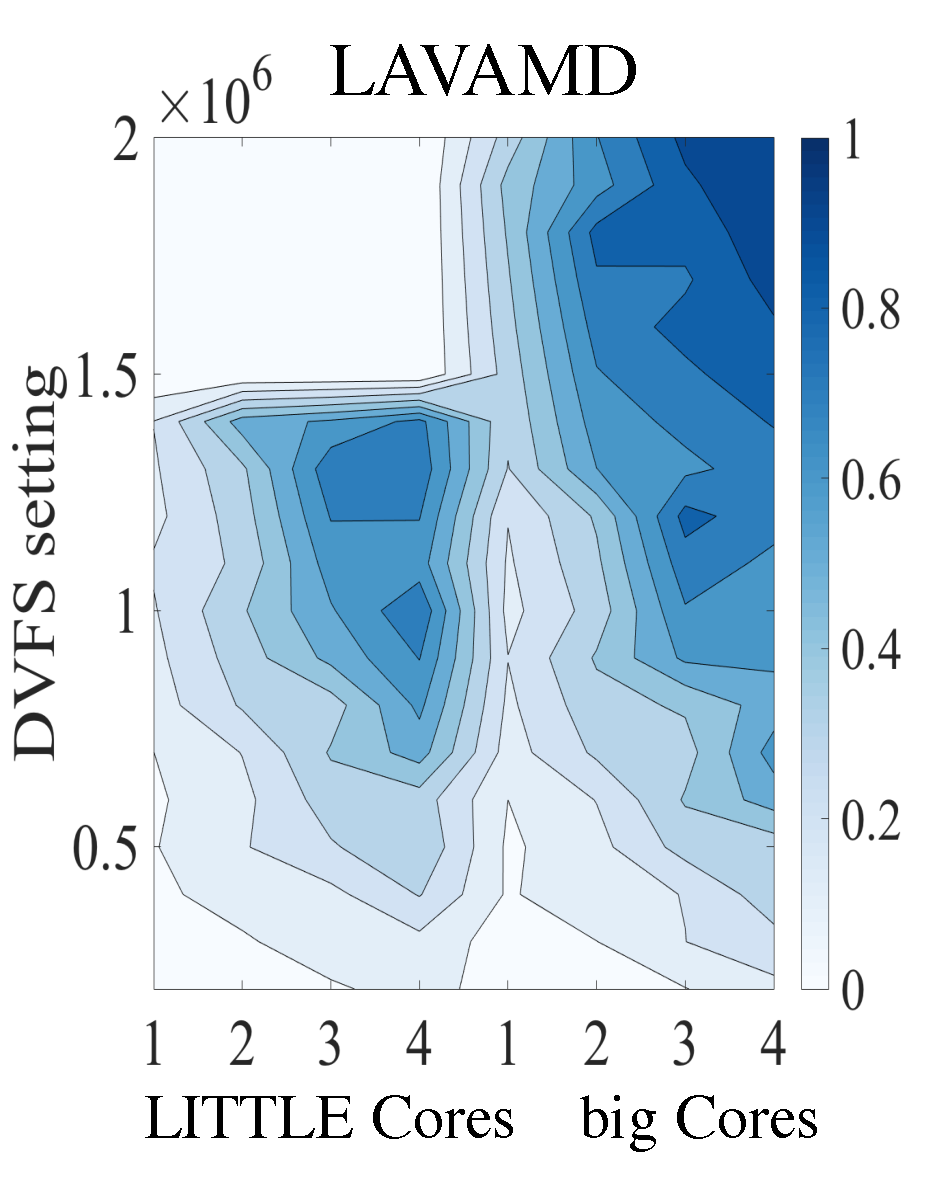
\includegraphics[width=.2\textwidth]{figures/lavamd2.pdf}
    \label{fig:lavamd}
  }
  \subfloat[]
  {
    \begin{tikzpicture}
\begin{centering}

\begin{groupplot}[
    group style={
        group name=plots,
        group size=1 by 2,
        xlabels at=edge bottom,
        xticklabels at=edge bottom,
        vertical sep=5pt
    },
height=3.2cm,
width=0.55\columnwidth,
xmajorgrids,
ymajorgrids,
grid style={dashed},
xmin=0,
xmax=500,
yticklabel pos=left,
enlargelimits=false,
tick align = outside,
tick style={white},
xticklabel shift={-5pt},
yticklabel shift={-5pt},
ylabel shift={-2pt},
ylabel style={align=center},
unbounded coords=jump,
]

\nextgroupplot[ylabel={\footnotesize Performance \\ (Normalized)}, % Performance
ytick={0.0,0.5,1.0,1.5,2.0},
yticklabels={,0.5,1.0,1.5,2.0},
yticklabel style={font=\footnotesize},
ymin=0,
ymax=2.0,
%legend entries={{$\mathsf{\SYSTEM{}-NO-POLE}$},{{$\mathsf{\SYSTEM{}-HBM}$}}},
legend entries={{\scriptsize $\mathsf{\SYSTEM{}-NO-POLE}$},{\scriptsize $\mathsf{\SYSTEM{}-HBM}$}},
%legend style={fill=none,draw=none,at={(0.5,1.5)},anchor=north,legend columns=1,
%line width=1pt},
legend style={draw=none,at={(0.5,1.6)},anchor=north,legend columns=4,line width=5pt},
%legend style={fill=none,draw=none,at={(0.5,1.5)},anchor=north,legend columns=1,line width=1pt}
]

\addplot[thick, solid, color=CALOREE-NP, mark=none,each nth point=5] table[x index=0,y index=1,col sep=space] {img/pole/leo-poet-np-LAVAMD.txt};
\addplot[thick, solid, color=HBM-ADAPT, mark=none,each nth point=5] table[x index=0,y index=1,col sep=space] {img/pole/leo-poet-LAVAMD.txt};
%\addplot[thick, dashed, black] coordinates {(250,0) (250, 2)};


\nextgroupplot[ylabel={\footnotesize Power \\ (Watts)}, % Power
ytick={0.0,2.0,4.0,6.0},
yticklabels={,2.0,4.0,6.0},
yticklabel style={font=\footnotesize},
ymin=0,
ymax=6.0,
xlabel={\footnotesize $time$ [frame]},
xlabel near ticks,
xticklabels={,0,100,200,300,400,500},
]

\addplot[thick, solid, color=CALOREE-NP, mark=none,smooth,each nth point=5] table[x index=0,y index=2,col sep=space] {img/pole/leo-poet-np-LAVAMD.txt};
\addplot[thick, solid, color=HBM-ADAPT, mark=none,smooth,each nth point=5] table[x index=0,y index=2,col sep=space] {img/pole/leo-poet-LAVAMD.txt};
%\addplot[thick, dashed, black] coordinates {(250,0) (250, 6)};
\end{groupplot}
\end{centering}

\end{tikzpicture}

    \label{fig:lavamd-pole}
  }
  \caption{(a) LAVAMD's performance with different resources. (b) The
    pole's effects on LAVAMD's behaviors.}
  \label{fig:lavamd-is-hard}
\end{figure}


%\begin{wrapfigure}{r}{0.5\columnwidth}
%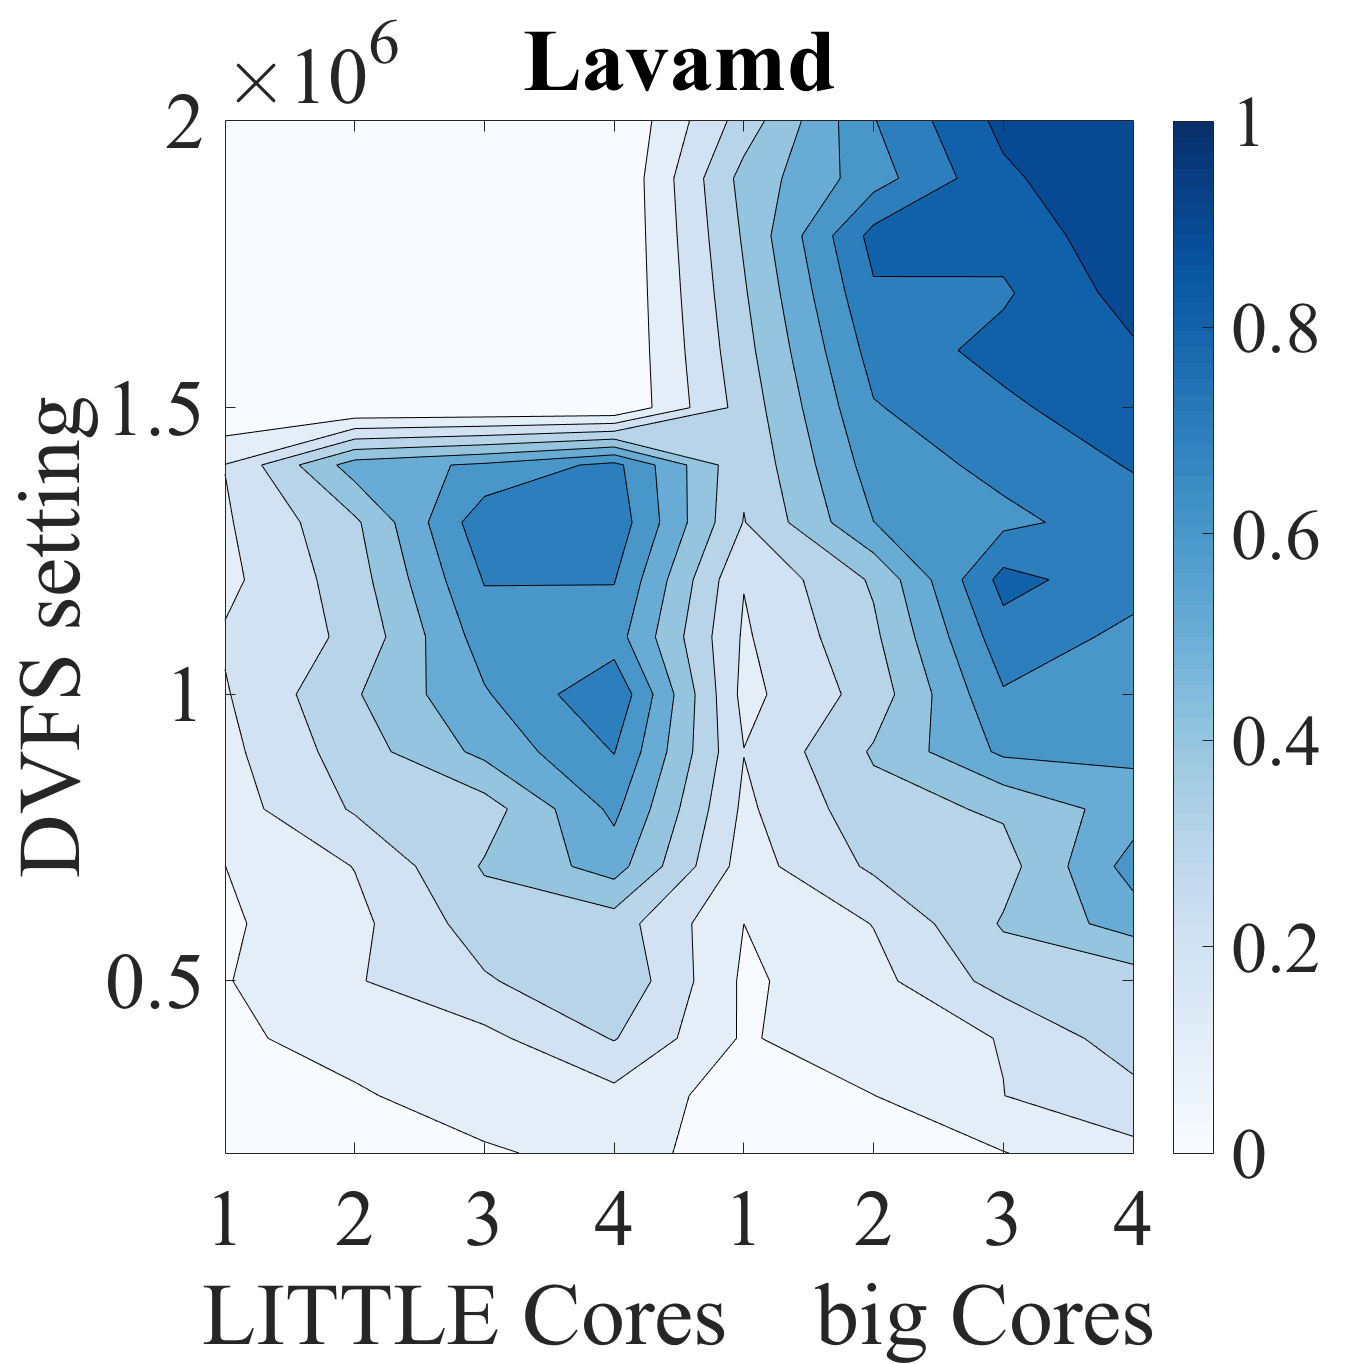
\includegraphics[width=.25\textwidth]{figures/lavamd.png}
%\caption{Performance of LAVAMD with differnt resources.}
%\label{fig:lavamd}
%\end{wrapfigure}
LAVAMD has one of the most complicated responses to resource usage on
our system with multiple local optima, as shown in
\figref{fig:lavamd}.  \secref{guarantees} presents an analytical
argument that tuning the controller to model variance and confidence
interval prevents oscillation and provide probabilistic control
theoretic guarantees despite using noisy, learned models to control
such complicated behavior.  We now demonstrate this empirically by
showing LAVAMD's single-app behavior controlled by both CALOREE-NoPole
and \SYSTEM{}-HBM to meet the 80\% target.

\figref{fig:lavamd-pole} shows the results, with time on the x-axis
and normalized performance and power on the respective y-axes.
CALOREE-NoPole oscillates around the desired performance and causes
wide fluctuations in power consumption.  In contrast, after receiving
the model from its learner, \SYSTEM{} provides reliable performance
right at the target value (normalized to 1 in this case).  \SYSTEM{}
also saves tremendous energy because it does not oscillate but uses a
mixture of big and LITTLE cores to keep energy near minimal.
% \TODO{Do we need the vertical line here?  This is a single app run
%   right?}

%\begin{figure}[t]
%  \begin{tikzpicture}
\begin{centering}

\begin{groupplot}[
    group style={
        group name=plots,
        group size=1 by 2,
        xlabels at=edge bottom,
        xticklabels at=edge bottom,
        vertical sep=5pt
    },
height=3.2cm,
width=0.55\columnwidth,
xmajorgrids,
ymajorgrids,
grid style={dashed},
xmin=0,
xmax=500,
yticklabel pos=left,
enlargelimits=false,
tick align = outside,
tick style={white},
xticklabel shift={-5pt},
yticklabel shift={-5pt},
ylabel shift={-2pt},
ylabel style={align=center},
unbounded coords=jump,
]

\nextgroupplot[ylabel={\footnotesize Performance \\ (Normalized)}, % Performance
ytick={0.0,0.5,1.0,1.5,2.0},
yticklabels={,0.5,1.0,1.5,2.0},
yticklabel style={font=\footnotesize},
ymin=0,
ymax=2.0,
%legend entries={{$\mathsf{\SYSTEM{}-NO-POLE}$},{{$\mathsf{\SYSTEM{}-HBM}$}}},
legend entries={{\scriptsize $\mathsf{\SYSTEM{}-NO-POLE}$},{\scriptsize $\mathsf{\SYSTEM{}-HBM}$}},
%legend style={fill=none,draw=none,at={(0.5,1.5)},anchor=north,legend columns=1,
%line width=1pt},
legend style={draw=none,at={(0.5,1.6)},anchor=north,legend columns=4,line width=5pt},
%legend style={fill=none,draw=none,at={(0.5,1.5)},anchor=north,legend columns=1,line width=1pt}
]

\addplot[thick, solid, color=CALOREE-NP, mark=none,each nth point=5] table[x index=0,y index=1,col sep=space] {img/pole/leo-poet-np-LAVAMD.txt};
\addplot[thick, solid, color=HBM-ADAPT, mark=none,each nth point=5] table[x index=0,y index=1,col sep=space] {img/pole/leo-poet-LAVAMD.txt};
%\addplot[thick, dashed, black] coordinates {(250,0) (250, 2)};


\nextgroupplot[ylabel={\footnotesize Power \\ (Watts)}, % Power
ytick={0.0,2.0,4.0,6.0},
yticklabels={,2.0,4.0,6.0},
yticklabel style={font=\footnotesize},
ymin=0,
ymax=6.0,
xlabel={\footnotesize $time$ [frame]},
xlabel near ticks,
xticklabels={,0,100,200,300,400,500},
]

\addplot[thick, solid, color=CALOREE-NP, mark=none,smooth,each nth point=5] table[x index=0,y index=2,col sep=space] {img/pole/leo-poet-np-LAVAMD.txt};
\addplot[thick, solid, color=HBM-ADAPT, mark=none,smooth,each nth point=5] table[x index=0,y index=2,col sep=space] {img/pole/leo-poet-LAVAMD.txt};
%\addplot[thick, dashed, black] coordinates {(250,0) (250, 6)};
\end{groupplot}
\end{centering}

\end{tikzpicture}

%   \vskip -.5em
%   \caption{The pole's effects on LAVAMD behavior.}
%  \label{fig:lavamd-pole}
%\end{figure}


\subsection{Sensitivity to the Measured Samples}
We vary the number of samples taken and show how it affects model
accuracy for the Online, Netflix, and HBM learners.  Accuracy is how
close the model is to ground truth (found through exhaustive
exploration), with 1 meaning the model perfectly reproduced the real
performance or power.  Accuracy is significant, because the smaller
the number of samples, the faster the controller can switch from a
general model to the learner's application-specific model.

\figref{fig:sensitivity} compares the Online, HBM, and Netflix
learners for both performance (top) and power (bottom).  The figure
shows sample size on the x-axis and accuracy on the y-axis.  The HBM
initially performs as well as Offline and as sample size increases,
the accuracy uniformly improves, exceeding 90\% after 20 samples. The
Online approach needs at least 7 samples before it can even generate a
model.  As Online receives more samples, its accuracy improves but
never exceeds HBM's for the same number of samples. Netflix is very
noisy for sample sizes, but once the number of samples reaches about
50, it is competitive with HBM.  These results not only demonstrate
the sensitivity to sample size, they show why \SYSTEM{}-HBM achieves
better results than the other learning mechanisms.

\begin{figure}[t]
  \begin{tikzpicture}
\begin{centering}
\pgfplotstableread[col sep=space]{img/sample_accuracy-v3.txt}{\datatable}
\begin{groupplot}[
    group style={
        group name=plots,
        group size=1 by 2,
        xlabels at=edge bottom,
        xticklabels at=edge bottom,
        vertical sep=5pt
    },
height=3.3cm,
width=0.95\columnwidth,
xmajorgrids,
ymajorgrids,
grid style={dashed},
xmin=0,
xmax=100,
yticklabel pos=left,
enlargelimits=false,
tick align = outside,
tick style={white},
xticklabel shift={-5pt},
yticklabel shift={-5pt},
ylabel shift={-2pt},
ylabel style={align=center},
unbounded coords=jump,
]

\nextgroupplot[ylabel={\footnotesize Accuracy\\(Performance)}, % Performance
xtick={0,20,40,60,80,100},
ytick={0.0,0.3,0.6,0.9},
yticklabels={,0.3,0.6,0.9},
yticklabel style={font=\footnotesize},
ymin=0,
ymax=1,
legend entries={{$\mathsf{ONLINE}$},{$\mathsf{HBM}$},{$\mathsf{NETFLIX}$}},
legend style={draw=none,at={(0.5,1.6)},anchor=north,legend columns=4,line width=5pt},
]
\addplot[thick, solid, color=ONLINE-ADAPT] table[x index=0,y index=3] {\datatable};
\addplot[thick, solid, color=HBM-ADAPT]    table[x index=0,y index=1] {\datatable};
\addplot[thick, solid, color=NUCLEAR-ADAPT]  table[x index=0,y index=7] {\datatable};

\nextgroupplot[ylabel={\footnotesize Accuracy\\ (Power)}, % Power
ytick={0.0,0.3,0.6,0.9,1.0},
yticklabels={,0.3,0.6,0.9,1.0},
yticklabel style={font=\footnotesize},
ymin=0,
ymax=1,
xlabel={\footnotesize \% Samples for training},
xlabel near ticks,
xtick={0,20,40,60,80,100},
xticklabels={0,20,40,60,80,100},
xticklabel style={font=\footnotesize},
]

\addplot[thick, solid, color=ONLINE-ADAPT]    table[x index=0,y index=4] {\datatable};
\addplot[thick, solid, color=HBM-ADAPT]   table[x index=0,y index=2] {\datatable};
\addplot[thick, solid, color=NUCLEAR-ADAPT] table[x index=0,y index=8] {\datatable};

\end{groupplot}
\end{centering}

\end{tikzpicture}

   \vskip -.5em
  \caption{Estimation accuracy versus sample size.}
  \label{fig:sensitivity}
\end{figure}

%\PUNT{

\subsection{Overhead}
\SYSTEM{}'s main source of overhead is sampling where the applications
need to run through a few configurations before \SYSTEM{} can reliably
estimate the entire power and performance frontier. We argue that the
sampling cost can be distributed across devices by asking each of them
to contribute samples for estimation. Once the sampling phase is over,
the HBM is quite fast and can generate an estimate as fast as 500 ms
which is significantly smaller than the time required to run any of
our applications.  Additionally, \SYSTEM{}'s asynchronous
communication means that the controller never waits for the learner.
Using the four ODROIDs in our experimental system, each board only
needs to contribute 4 samples to achieve 90\% accuracy.  In the worst
case (\texttt{facesim}), this sampling overhead is less than 2\%.  For
all other benchmarks it is lower, and for most it is negligible.

The controller requires only a few floating point operations to
execute, plus the table lookups in the PHT.  To evaluate its overhead,
we time 1000 iterations.  We find that it is under 2 microseconds,
which is significantly faster than we can change any resource
allocation on our system.  We conclude that the controller has
negligible impact on performance and energy consumption of the
controlled device.

\section{Related Work}

We discuss related work in managing resources to meet performance
goals and reduce energy.  

\subsection{Machine Learning}
We break learning for resource management into 3 categories: offline,
online, and hybrid approaches.

\noindent \textbf{Offline Learning} These approaches build models
before deployment and then use those fixed models to allocate
resources
\cite{Yi2003,LeeBrooks2006,CPR,ChenJohn2011,petabricksStatic}.  The
model-building phase is expensive, requiring both a large number of
samples and substantial computation.  Applying the model online,
however, is low overhead.  The main drawback is that the models are
not updated as the system runs: a problem for adapting workloads.
\PUNT{A good example of an offline approach applies learning to render
  web pages on mobile systems with low energy \cite{reddiHPCA2013}. It
  builds an offline model mapping web page features into performance
  for different core types.  When a new page is downloaded, the system
  estimates the resources needed to render the web page and uses the
  lowest energy configuration that meets user satisfaction.  This
  approach handles the complexity of allocating resources to webpage
  rendering, but cannot address dynamics; \eg{} when other apps run
  concurrently with the web browser.}  Carat is a good example of an
offline learner that aggregates data across multiple devices to
generate a report for human users about how to configure their device
to increase battery life \cite{carat}.  While both Carat and \SYSTEM{}
learn across devices, they have very different goals.  Carat returns
very high-level information to human users; \eg{} update a driver to
extend battery life.  \SYSTEM{} automatically builds and applies
low-level models to save energy.

\noindent \textbf{Online Learning} Online techniques observe the
current application to tune system resource usage for that application
\cite{Li2006,Flicker,ParallelismDial,Ponamarev,petabricksDynamic,LeeBrooks}.
For example, Flicker is a configurable architecture and optimization
framework that uses online models to maximize performance under a
power limitation \cite{Flicker}.  Another example, ParallelismDial,
uses online adaptation to tailor parallelism to application workload
\cite{ParallelismDial}.



\noindent \textbf{Hybrid Approaches} Some approaches combine offline
predictive models with online adaptation
\cite{Zhang2012,packandcap,Winter2010,dubach2010,Koala,Cinder,
  wu2012inferred}.  For example, Dubach et al.  use hybrid models to
optimize the microarchitecture of a single core \cite{dubach2010}.
Such predictive models have also been employed at the operating system
level to manage system energy consumption
\cite{Koala,Cinder,wu2012inferred}.  Other approaches combine offline
modeling with online updates \cite{JouleGuard,Bitirgen2008,Ipek}.  For
example, Bitirgen et al use an artificial neural network to allocate
resources to multiple applications in a multicore \cite{Bitirgen2008}.
The neural network is trained offline and then adapted online using
measured feedback.  This approach maximizes performance but does not
consider power or energy minimization.

\subsection{Control}
Almost all control solutions can be thought of as a combination of
offline model building with online adaptation.  The model building
involves substantial empirical measurement that is used to synthesize
a control system
\cite{Wu2004,TCST,Chen2011,PTRADE,POET,ControlWare,Agilos,Rajkumar,Sojka,Raghavendra2008}.
The combination of offline learning and control works well over a
narrow range of applications, as the offline models capture the
general behavior of a class of application and require negligible
online overhead.  This focused approach is extremely effective for
multimedia applications \cite{grace2,flinn99,flinn2004,xtune,TCST} and
web-servers \cite{Horvarth,LuEtAl-2006a,SunDaiPan-2008a} because the
workloads can be characterized ahead of time so that the models
produce sound control.

Indeed, the need for good models is the central tension in developing
control for computing systems.  It is always possible to build a
controller for a specific application and system by extensively
modeling that pair.  More general controllers, which work with a range
of applications, have addressed the need for models in various ways.
Some provide libraries that encapsulate control functionality and
require user-specified models
\cite{ControlWare,Sojka,Rajkumar,POET,SWiFT}.  Others automatically
synthesize both a model and a controller for either hardware
\cite{josep-isca2016} or software \cite{ICSE2014,FSE2015}.  JouleGuard
combines learning for energy efficiency with control for managing
application parameters \cite{JouleGuard}.  In JouleGuard, a learner
adapts the controller's coefficients to model uncertainty, but
JouleGuard's learner does not produce a new model for the controller.
Because JouleGuard's learner runs on the same device as the controlled
application, it must be computationally efficient and thus it cannot
identify correlations across applications or even different resource
configurations.  \SYSTEM{} is unique in that a separate learner
generates an application-specific model automatically.  By offloading
the learning task, \SYSTEM{} (1) combines data from many applications
and systems and (2) applies computationally expensive, but highly
accurate learning techniques.



\section{Summary}
While much recent work has built systems to support learning and big
data, in this work we use learning and big data to build better
systems.  Specifically by proposing \SYSTEM{}, a combination of
machine learning and control for managing resources to meet
performance requirements with minimal energy.  \SYSTEM{}'s unique
contribution is showing how machine learning and control theory can be
combined at runtime to provide more reliable performance and lower
energy than either in isolation.  Furthermore, this combination is not
just practical, it provides formal guarantees that the system will
converge to the desired performance.

\appendix
\subsection*{Probabilistic Convergence Guarantees}


\begin{thm}
  Let $\mathbf{s}$ and $\hat{\mathbf{s}}$ denote the true and estimated speedups of various configurations in set $C$ as $\mathbf{s} \in \mathbb{R}^{|C|}$. Let $\sigma$ denote the
  estimation error for speedups such that, $\hat{s_i} \sim
  N(s_i, \sigma^2)$ $\forall$ $i$. We can show that with probability
  greater than 99.7\%, the pole $\rho(t)$ can be chosen to lie in the range, $[\Floor{1- \Floor{max(\hat{s})/(min(\hat{s}) -  3\sigma)}_0}_0, 1)$, where $\Floor{x}_0 = \max(x,0)$.
\end{thm}

\begin{proof}
Let $\Delta$ denote the multiplicative error over speedups, such that $ \widehat{speedup(t)}\Delta = speedup(t) $. To
guarantee convergence the value of pole, $\rho(t)$ can vary in the range
$\Floor{1-\frac{2}{\Delta})}_0, 1)$\cite{ICSE2014}. The lowest value of $\rho(t)$ offer the fastest convergence. We have described in Equations \ref{eqn:s1} \& \ref{eqn:s2} that any speedup can be written as a linear combination of two configuration speedups as,

\begin{align}
speedup(t) = \hat{s}_{hi} \cdot \tau_{hi} + \hat{s}_{lo} \cdot (T - \tau_{hi})
\end{align}
\begin{align}
\widehat{speedup}(t) = s_{hi} \cdot \tau_{hi} + s_{lo} \cdot (T - \tau_{hi})
\end{align}

We can upper bound and lower bound each of these terms,
\begin{align}
speedup(t) \leq T \hat{s}_{hi} \;\; \text{and} \;\; \widehat{speedup}(t) \geq T s_{lo}
\end{align}

The estimates of speedups are close to the actual speedups since
$\hat{s} \sim N(s, \sigma^2)$, therefore with probability greater
than 99.7\% and the speedups can be given by, $s_{lo} \geq
\hat{s}_{lo} - 3 \sigma$. Hence, $\widehat{speedup}(t) \geq T
(\hat{s}_{lo} -3 \sigma)$. Since, over all configurations, $\Delta \leq
\Floor{max(\hat{s})/(min(\hat{s}) - 3\sigma)}_0$,  we can choose the pole from the range,  $([\Floor{1- \Floor{max(\hat{s})/(min(\hat{s}) - 3\sigma)}_0}_0, 1)$.


\end{proof}


\makebibliography

% Figures and tables, if you decide to leave them to the end
%\input{figure}
%\input{table}

\end{document}
